%%%%%%%%%%%%%%%%%%%%%%%%%%%%%%%%%%%%%%%%%%%%%%%%%%%%%%%%%%%%%%%%%%%%%%%%%%%%%%%%
% May 2022 - This template was prepared by Dorothea F. Brosius of the Institute
% for Electronics and Applied Physics, University of Maryland, College Park, MD
% To be used with when typing your own bibliography or when using Bibtex files
%
% The template was last updated in January 2022 - margins changed to 1 inch on
% all sides Thesis Main Page used with thesis.sty based on the University of
% Maryland Electronic Thesis and Dissertation (ETD) Style Guide, 2021 Edition
%%%%%%%%%%%%%%%%%%%%%%%%%%%%%%%%%%%%%%%%%%%%%%%%%%%%%%%%%%%%%%%%%%%%%%%%%%%%%%%%

% Select the version that fits how you are making this LaTeX document (its
% driver). The first two are the most likely ones to be needed.
\newcommand{\mydriver}{pdflatex} %Making a PDF directly using pdflatex.
\documentclass[12pt,\mydriver]{thesis}  %12pt is larger than 11pt

% packages %%%%%%%%%%%%%%%%%%%%%%%%%%%%%%%%%%%%%%%%%%%%%%%%%%%%%%%%%%%%%%%%%%%%%

%%%%%%%%%%%%
% graphics %
%%%%%%%%%%%%
\usepackage{tikz}
\usetikzlibrary{external}
\tikzexternalize[prefix=cache/]

\usetikzlibrary{arrows.meta,
                calc,
                chains,
                quotes,
                positioning,
                shapes.geometric}

\usepackage{graphicx}


%%%%%%%%%%
% floats %
%%%%%%%%%%
\usepackage{float}
\usepackage{caption}
\usepackage{subcaption}
%\usepackage{wrapfig}

% Don't float across chapters!
\usepackage[above,below]{placeins}


%%%%%%%%%%%%%%%%%%%%%%
% general appearance %
%%%%%%%%%%%%%%%%%%%%%%
\usepackage{titlesec}
\titleformat{\chapter}{\normalfont\large}{\chaptername\ \thechapter:}{1em}{}

% indent first paragraph after section header
\usepackage{indentfirst}

% Times New Roman maybe, probably should switch to newtx
%\usepackage{times}

% some special symbols?
%\usepackage{latexsym}

% use cm super
\usepackage[T1]{fontenc}

% adds space between chapter/appendix and title in toc
\usepackage{titletoc,tocloft,calc}
\renewcommand{\cftlottitlefont}{\hspace*{\fill}\large}
\renewcommand{\cftloftitlefont}{\hspace*{\fill}\large}
\renewcommand{\cftafterlottitle}{\hspace*{\fill}}
\renewcommand{\cftafterloftitle}{\hspace*{\fill}}

\renewcommand{\cftchappresnum}{\chaptername\space}
\renewcommand{\cftchapaftersnum}{:\space}
\setlength{\cftchapnumwidth}{\widthof{\bfseries Chapter~99:~}}

\makeatletter
\g@addto@macro\appendix{%
    \renewcommand{\chaptername}{Appendix}
}
\makeatother

% better typesetting
\usepackage{microtype}


%%%%%%%%%%
% layout %
%%%%%%%%%%
\usepackage{lscape}
%\usepackage{multirow}


%%%%%%%%%%
% tables %
%%%%%%%%%%

% better vertical spacing in tables and arrays
\usepackage{tabls}

% slash cell for tables
%\usepackage{slashbox}

% longtables and alternatives
\usepackage{longtable}
\usepackage{supertabular}

% multi-line cell
\usepackage{makecell}

% continuous vertical line w/ booktabs
\usepackage{booktabs}
\aboverulesep=0ex
\belowrulesep=0ex
\renewcommand{\arraystretch}{1.28}

% parnote inside floating table
\usepackage[symbol,restart,breakwithin]{parnotes}


%%%%%%%%
% math %
%%%%%%%%
\usepackage{amsmath}
\usepackage{amssymb}
\usepackage{amsfonts}


%%%%%%%%%%%%%%%%%%%%%%%%%
% citations, links, etc %
%%%%%%%%%%%%%%%%%%%%%%%%%
\usepackage[pdfencoding=auto,psdextra]{hyperref}
\hypersetup{breaklinks,citecolor=blue}
\usepackage{cleveref}

% bibliography
% \usepackage[sort,square,numbers]{natbib}
\usepackage[
    %style=phys,
    giveninits=true,
    %backref=true,
    natbib=true,
    backend=biber,
    doi=false,
    % Sort by the order of citation
    sorting=none,
    % This options ensures that no automatic et al. is generated
    %maxbibnames=99,
    % This option must be enabled with 'babel' package
    useprefix=false
]{biblatex}
\addbibresource{external.bib}
\addbibresource{LHCb-MISC.bib}
\addbibresource{LHCb-PAPER.bib}

% used for placing bibliography after each chapter
%\usepackage[sectionbib]{chapterbib}
%\usepackage{bibentry}

% citation: Ref. [n]
\let\oldcite\cite
\renewcommand{\cite}[1]{Ref.~\oldcite{#1}}


%%%%%%%%%%%%%%%%%%%%%%%%
% geometry and spacing %
%%%%%%%%%%%%%%%%%%%%%%%%
\usepackage{setspace}

% margins
\setlength{\textwidth}{6.4in}
\setlength{\textheight}{9in}
\setlength{\topmargin}{-.55in}
%\setlength{\topmargin}{0in}    % use this setting if the printer makes the top margin 1/2 inch instead of 1 inch
\setlength{\oddsidemargin}{.1in}   % sets left margin to 1 inch
\setlength{\parindent}{.4in}

% Always single-space equations
\usepackage{etoolbox}
\BeforeBeginEnvironment{equation}{\begin{singlespace}}
\AfterEndEnvironment{equation}{\end{singlespace}\noindent\ignorespaces}
\BeforeBeginEnvironment{align}{\begin{singlespace}}
\AfterEndEnvironment{align}{\end{singlespace}\noindent\ignorespaces}


%%%%%%%%
% misc %
%%%%%%%%
\usepackage{xspace}

% hyphenation
\usepackage[english]{babel}
\hyphenation{
    tem-po-ral-ly
    pro-cesses
    ex-pe-ri-men-tal-ly
    fluc-tua-tions
    si-mu-la-tions
}

% automatically bold math when using \bfseries command
% this is very useful for section headings
\makeatletter
\g@addto@macro\bfseries{\boldmath}
\makeatother

\newcommand{\smalltt}[1]{{\small\texttt{#1}}}

% commands for technical links (might want to disable them all together)
\newcommand{\techlink}[1]{For info on related code/software, see \cref{#1}.}
\newcommand{\techurllink}[2]{\href{#1}{\nolinkurl{#2}}}

% graphics base paths
\graphicspath{{./appendix}{./chapter}{./addon}}


% include %%%%%%%%%%%%%%%%%%%%%%%%%%%%%%%%%%%%%%%%%%%%%%%%%%%%%%%%%%%%%%%%%%%%%%

%%%%%%%%%%%%%%%%%%%%%%%%%%%%%%%%%%%%%%%%%%%%%%%%%%%%%%%%%%%%%%%%%%%%%%%%
%%%                                                                    %
%%% !!!!!!!!!!!!!!!!!!! DO NOT EDIT THIS FILE !!!!!!!!!!!!!!!!!!!!!!!! %
%%%                                                                    %
%%% THE EB MAY OVERWRITE IT TO REFLECT LATEST CHANGES IN THE TEMPLATE  %
%%%                                                                    %
%%% You may define your own macros and packages in main.tex or add     %
%%% additional local files                                             %
%%%%%%%%%%%%%%%%%%%%%%%%%%%%%%%%%%%%%%%%%%%%%%%%%%%%%%%%%%%%%%%%%%%%%%%%
%%% ======================================================================
%%% Purpose: Standard LHCb aliases
%%% Author: Originally Ulrik Egede, adapted by Tomasz Skwarnicki for templates,
%%% rewritten by Chris Parkes
%%% Maintainer : Ulrik Egede (2010 - 2012)
%%% Maintainer : Rolf Oldeman (2012 - 2014)
%%% Maintainer : Patrick Koppenburg (2018--2020)
%%% =======================================================================
%%% To use this file outside the normal LHCb document environment, the
%%% following should be added in a preamble (before \begin{document}
%%%
\usepackage{ifthen}
\newboolean{uprightparticles}
\setboolean{uprightparticles}{false} %Set true for upright particle symbols
\usepackage{xspace}
\usepackage{upgreek}


%%%%%%%%%%%%%%%%%%%%%%%%%%%%%%%%%%%%%%%%%%%%%%%%%%%%%%%%%%%%
%%%
%%% The following is to ensure that the template automatically can process
%%% this file.
%%%
%%% Add comments with at least three %%% preceding.
%%% Add new sections with one % preceding
%%% Add new subsections with two %% preceding
%%%
%%% For upper greek letters, Xires and Xiresbar will be the particles without the charge
%%% States with charge are called Xiz and Xim
%%%
%%%%%%%%%%%%%%%%%%%%%%%%%%%%%%%%%%%%%%%%%%%%%%%%%%%%%%%%%%%%

%%%%%%%%%%%%%
% Experiments
%%%%%%%%%%%%%
\def\lhcb   {\mbox{LHCb}\xspace}
\def\atlas  {\mbox{ATLAS}\xspace}
\def\cms    {\mbox{CMS}\xspace}
\def\alice  {\mbox{ALICE}\xspace}
\def\babar  {\mbox{BaBar}\xspace}
\def\belle  {\mbox{Belle}\xspace}
\def\belletwo {\mbox{Belle~II}\xspace}
\def\besiii {\mbox{BESIII}\xspace}
\def\cleo   {\mbox{CLEO}\xspace}
\def\cdf    {\mbox{CDF}\xspace}
\def\dzero  {\mbox{D0}\xspace}
\def\aleph  {\mbox{ALEPH}\xspace}
\def\delphi {\mbox{DELPHI}\xspace}
\def\opal   {\mbox{OPAL}\xspace}
\def\lthree {\mbox{L3}\xspace}
\def\sld    {\mbox{SLD}\xspace}
%%%\def\argus  {\mbox{ARGUS}\xspace}
%%%\def\uaone  {\mbox{UA1}\xspace}
%%%\def\uatwo  {\mbox{UA2}\xspace}
%%%\def\ux85 {\mbox{UX85}\xspace}
\def\cern {\mbox{CERN}\xspace}
\def\lhc    {\mbox{LHC}\xspace}
\def\lep    {\mbox{LEP}\xspace}
\def\tevatron {Tevatron\xspace}
\def\bfactories {\mbox{\B Factories}\xspace}
\def\bfactory   {\mbox{\B Factory}\xspace}
\def\upgradeone {\mbox{Upgrade~I}\xspace}
\def\upgradetwo {\mbox{Upgrade~II}\xspace}

%% LHCb sub-detectors and sub-systems

%%%\def\pu     {PU\xspace}
\def\velo   {VELO\xspace}
\def\rich   {RICH\xspace}
\def\richone {RICH1\xspace}
\def\richtwo {RICH2\xspace}
\def\ttracker {TT\xspace}
\def\intr   {IT\xspace}
\def\st     {ST\xspace}
\def\ot     {OT\xspace}
\def\herschel {\mbox{\textsc{HeRSCheL}}\xspace}
%%%\def\Tone   {T1\xspace}
%%%\def\Ttwo   {T2\xspace}
%%%\def\Tthree {T3\xspace}
%%%\def\Mone   {M1\xspace}
%%%\def\Mtwo   {M2\xspace}
%%%\def\Mthree {M3\xspace}
%%%\def\Mfour  {M4\xspace}
%%%\def\Mfive  {M5\xspace}
\def\spd    {SPD\xspace}
\def\presh  {PS\xspace}
\def\ecal   {ECAL\xspace}
\def\hcal   {HCAL\xspace}
%%%\def\bcm    {BCM\xspace}
\def\MagUp {\mbox{\em Mag\kern -0.05em Up}\xspace}
\def\MagDown {\mbox{\em MagDown}\xspace}

\def\ode    {ODE\xspace}
\def\daq    {DAQ\xspace}
\def\tfc    {TFC\xspace}
\def\ecs    {ECS\xspace}
\def\lone   {L0\xspace}
\def\hlt    {HLT\xspace}
\def\hltone {HLT1\xspace}
\def\hlttwo {HLT2\xspace}

%%% Upright (not slanted) Particles

\ifthenelse{\boolean{uprightparticles}}%
{\def\Palpha      {\ensuremath{\upalpha}\xspace}
 \def\Pbeta       {\ensuremath{\upbeta}\xspace}
 \def\Pgamma      {\ensuremath{\upgamma}\xspace}
 \def\Pdelta      {\ensuremath{\updelta}\xspace}
 \def\Pepsilon    {\ensuremath{\upepsilon}\xspace}
 \def\Pvarepsilon {\ensuremath{\upvarepsilon}\xspace}
 \def\Pzeta       {\ensuremath{\upzeta}\xspace}
 \def\Peta        {\ensuremath{\upeta}\xspace}
 \def\Ptheta      {\ensuremath{\uptheta}\xspace}
 \def\Pvartheta   {\ensuremath{\upvartheta}\xspace}
 \def\Piota       {\ensuremath{\upiota}\xspace}
 \def\Pkappa      {\ensuremath{\upkappa}\xspace}
 \def\Plambda     {\ensuremath{\uplambda}\xspace}
 \def\Pmu         {\ensuremath{\upmu}\xspace}
 \def\Pnu         {\ensuremath{\upnu}\xspace}
 \def\Pxi         {\ensuremath{\upxi}\xspace}
 \def\Ppi         {\ensuremath{\uppi}\xspace}
 \def\Pvarpi      {\ensuremath{\upvarpi}\xspace}
 \def\Prho        {\ensuremath{\uprho}\xspace}
 \def\Pvarrho     {\ensuremath{\upvarrho}\xspace}
 \def\Ptau        {\ensuremath{\uptau}\xspace}
 \def\Pupsilon    {\ensuremath{\upupsilon}\xspace}
 \def\Pphi        {\ensuremath{\upphi}\xspace}
 \def\Pvarphi     {\ensuremath{\upvarphi}\xspace}
 \def\Pchi        {\ensuremath{\upchi}\xspace}
 \def\Ppsi        {\ensuremath{\uppsi}\xspace}
 \def\Pomega      {\ensuremath{\upomega}\xspace}

 \def\PDelta      {\ensuremath{\Delta}\xspace}
 \def\PXi         {\ensuremath{\Xi}\xspace}
 \def\PLambda     {\ensuremath{\Lambda}\xspace}
 \def\PSigma      {\ensuremath{\Sigma}\xspace}
 \def\POmega      {\ensuremath{\Omega}\xspace}
 \def\PUpsilon    {\ensuremath{\Upsilon}\xspace}
 \let\oldPi\Pi
 \def\PPi         {\ensuremath{\oldPi}\xspace}


 \def\PA      {\ensuremath{\mathrm{A}}\xspace}
 \def\PB      {\ensuremath{\mathrm{B}}\xspace}
 \def\PC      {\ensuremath{\mathrm{C}}\xspace}
 \def\PD      {\ensuremath{\mathrm{D}}\xspace}
 \def\PE      {\ensuremath{\mathrm{E}}\xspace}
 \def\PF      {\ensuremath{\mathrm{F}}\xspace}
 \def\PG      {\ensuremath{\mathrm{G}}\xspace}
 \def\PH      {\ensuremath{\mathrm{H}}\xspace}
 \def\PI      {\ensuremath{\mathrm{I}}\xspace}
 \def\PJ      {\ensuremath{\mathrm{J}}\xspace}
 \def\PK      {\ensuremath{\mathrm{K}}\xspace}
 \def\PL      {\ensuremath{\mathrm{L}}\xspace}
 \def\PM      {\ensuremath{\mathrm{M}}\xspace}
 \def\PN      {\ensuremath{\mathrm{N}}\xspace}
 \def\PO      {\ensuremath{\mathrm{O}}\xspace}
 \def\PP      {\ensuremath{\mathrm{P}}\xspace}
 \def\PQ      {\ensuremath{\mathrm{Q}}\xspace}
 \def\PR      {\ensuremath{\mathrm{R}}\xspace}
 \def\PS      {\ensuremath{\mathrm{S}}\xspace}
 \def\PT      {\ensuremath{\mathrm{T}}\xspace}
 \def\PU      {\ensuremath{\mathrm{U}}\xspace}
 \def\PV      {\ensuremath{\mathrm{V}}\xspace}
 \def\PW      {\ensuremath{\mathrm{W}}\xspace}
 \def\PX      {\ensuremath{\mathrm{X}}\xspace}
 \def\PY      {\ensuremath{\mathrm{Y}}\xspace}
 \def\PZ      {\ensuremath{\mathrm{Z}}\xspace}
 \def\Pa      {\ensuremath{\mathrm{a}}\xspace}
 \def\Pb      {\ensuremath{\mathrm{b}}\xspace}
 \def\Pc      {\ensuremath{\mathrm{c}}\xspace}
 \def\Pd      {\ensuremath{\mathrm{d}}\xspace}
 \def\Pe      {\ensuremath{\mathrm{e}}\xspace}
 \def\Pf      {\ensuremath{\mathrm{f}}\xspace}
 \def\Pg      {\ensuremath{\mathrm{g}}\xspace}
 \def\Ph      {\ensuremath{\mathrm{h}}\xspace}
 \def\Pi      {\ensuremath{\mathrm{i}}\xspace}
 \def\Pj      {\ensuremath{\mathrm{j}}\xspace}
 \def\Pk      {\ensuremath{\mathrm{k}}\xspace}
 \def\Pl      {\ensuremath{\mathrm{l}}\xspace}
 \def\Pm      {\ensuremath{\mathrm{m}}\xspace}
 \def\Pn      {\ensuremath{\mathrm{n}}\xspace}
 \def\Po      {\ensuremath{\mathrm{o}}\xspace}
 \def\Pp      {\ensuremath{\mathrm{p}}\xspace}
 \def\Pq      {\ensuremath{\mathrm{q}}\xspace}
 \def\Pr      {\ensuremath{\mathrm{r}}\xspace}
 \def\Ps      {\ensuremath{\mathrm{s}}\xspace}
 \def\Pt      {\ensuremath{\mathrm{t}}\xspace}
 \def\Pu      {\ensuremath{\mathrm{u}}\xspace}
 \def\Pv      {\ensuremath{\mathrm{v}}\xspace}
 \def\Pw      {\ensuremath{\mathrm{w}}\xspace}
 \def\Px      {\ensuremath{\mathrm{x}}\xspace}
 \def\Py      {\ensuremath{\mathrm{y}}\xspace}
 \def\Pz      {\ensuremath{\mathrm{z}}\xspace}
 \def\thebaroffset{0.0em}
}
{\def\Palpha      {\ensuremath{\alpha}\xspace}
 \def\Pbeta       {\ensuremath{\beta}\xspace}
 \def\Pgamma      {\ensuremath{\gamma}\xspace}
 \def\Pdelta      {\ensuremath{\delta}\xspace}
 \def\Pepsilon    {\ensuremath{\epsilon}\xspace}
 \def\Pvarepsilon {\ensuremath{\varepsilon}\xspace}
 \def\Pzeta       {\ensuremath{\zeta}\xspace}
 \def\Peta        {\ensuremath{\eta}\xspace}
 \def\Ptheta      {\ensuremath{\theta}\xspace}
 \def\Pvartheta   {\ensuremath{\vartheta}\xspace}
 \def\Piota       {\ensuremath{\iota}\xspace}
 \def\Pkappa      {\ensuremath{\kappa}\xspace}
 \def\Plambda     {\ensuremath{\lambda}\xspace}
 \def\Pmu         {\ensuremath{\mu}\xspace}
 \def\Pnu         {\ensuremath{\nu}\xspace}
 \def\Pxi         {\ensuremath{\xi}\xspace}
 \def\Ppi         {\ensuremath{\pi}\xspace}
 \def\Pvarpi      {\ensuremath{\varpi}\xspace}
 \def\Prho        {\ensuremath{\rho}\xspace}
 \def\Pvarrho     {\ensuremath{\varrho}\xspace}
 \def\Ptau        {\ensuremath{\tau}\xspace}
 \def\Pupsilon    {\ensuremath{\upsilon}\xspace}
 \def\Pphi        {\ensuremath{\phi}\xspace}
 \def\Pvarphi     {\ensuremath{\varphi}\xspace}
 \def\Pchi        {\ensuremath{\chi}\xspace}
 \def\Ppsi        {\ensuremath{\psi}\xspace}
 \def\Pomega      {\ensuremath{\omega}\xspace}
 \mathchardef\PDelta="7101
 \mathchardef\PXi="7104
 \mathchardef\PLambda="7103
 \mathchardef\PSigma="7106
 \mathchardef\POmega="710A
 \mathchardef\PUpsilon="7107
 \mathchardef\PPi="7105
 \def\PA      {\ensuremath{A}\xspace}
 \def\PB      {\ensuremath{B}\xspace}
 \def\PC      {\ensuremath{C}\xspace}
 \def\PD      {\ensuremath{D}\xspace}
 \def\PE      {\ensuremath{E}\xspace}
 \def\PF      {\ensuremath{F}\xspace}
 \def\PG      {\ensuremath{G}\xspace}
 \def\PH      {\ensuremath{H}\xspace}
 \def\PI      {\ensuremath{I}\xspace}
 \def\PJ      {\ensuremath{J}\xspace}
 \def\PK      {\ensuremath{K}\xspace}
 \def\PL      {\ensuremath{L}\xspace}
 \def\PM      {\ensuremath{M}\xspace}
 \def\PN      {\ensuremath{N}\xspace}
 \def\PO      {\ensuremath{O}\xspace}
 \def\PP      {\ensuremath{P}\xspace}
 \def\PQ      {\ensuremath{Q}\xspace}
 \def\PR      {\ensuremath{R}\xspace}
 \def\PS      {\ensuremath{S}\xspace}
 \def\PT      {\ensuremath{T}\xspace}
 \def\PU      {\ensuremath{U}\xspace}
 \def\PV      {\ensuremath{V}\xspace}
 \def\PW      {\ensuremath{W}\xspace}
 \def\PX      {\ensuremath{X}\xspace}
 \def\PY      {\ensuremath{Y}\xspace}
 \def\PZ      {\ensuremath{Z}\xspace}
 \def\Pa      {\ensuremath{a}\xspace}
 \def\Pb      {\ensuremath{b}\xspace}
 \def\Pc      {\ensuremath{c}\xspace}
 \def\Pd      {\ensuremath{d}\xspace}
 \def\Pe      {\ensuremath{e}\xspace}
 \def\Pf      {\ensuremath{f}\xspace}
 \def\Pg      {\ensuremath{g}\xspace}
 \def\Ph      {\ensuremath{h}\xspace}
 \def\Pi      {\ensuremath{i}\xspace}
 \def\Pj      {\ensuremath{j}\xspace}
 \def\Pk      {\ensuremath{k}\xspace}
 \def\Pl      {\ensuremath{l}\xspace}
 \def\Pm      {\ensuremath{m}\xspace}
 \def\Pn      {\ensuremath{n}\xspace}
 \def\Po      {\ensuremath{o}\xspace}
 \def\Pp      {\ensuremath{p}\xspace}
 \def\Pq      {\ensuremath{q}\xspace}
 \def\Pr      {\ensuremath{r}\xspace}
 \def\Ps      {\ensuremath{s}\xspace}
 \def\Pt      {\ensuremath{t}\xspace}
 \def\Pu      {\ensuremath{u}\xspace}
 \def\Pv      {\ensuremath{v}\xspace}
 \def\Pw      {\ensuremath{w}\xspace}
 \def\Px      {\ensuremath{x}\xspace}
 \def\Py      {\ensuremath{y}\xspace}
 \def\Pz      {\ensuremath{z}\xspace}
 \def\thebaroffset{0.18em}
}
\newcommand{\offsetoverline}[2][\thebaroffset]{\kern #1\overline{\kern -#1 #2}}%

%%%%%%%%%%%%%%%%%%%%%%%%%%%%%%%%%%%%%%%%%%%%%%%
% Particles
\makeatletter
\ifcase \@ptsize \relax% 10pt
  \newcommand{\miniscule}{\@setfontsize\miniscule{4}{5}}% \tiny: 5/6
\or% 11pt
  \newcommand{\miniscule}{\@setfontsize\miniscule{5}{6}}% \tiny: 6/7
\or% 12pt
  \newcommand{\miniscule}{\@setfontsize\miniscule{5}{6}}% \tiny: 6/7
\fi
\makeatother


\DeclareRobustCommand{\optbar}[1]{\shortstack{{\miniscule (\rule[.5ex]{1.25em}{.18mm})}
  \\ [-.7ex] $#1$}}


%% Leptons

\let\emi\en
\def\electron   {{\ensuremath{\Pe}}\xspace}
\def\en         {{\ensuremath{\Pe^-}}\xspace}   % electron negative (\em is taken)
\def\ep         {{\ensuremath{\Pe^+}}\xspace}
\def\epm        {{\ensuremath{\Pe^\pm}}\xspace}
\def\emp        {{\ensuremath{\Pe^\mp}}\xspace}
\def\epem       {{\ensuremath{\Pe^+\Pe^-}}\xspace}
%%%\def\ee         {\ensuremath{\Pe^-\Pe^-}\xspace}

\def\muon       {{\ensuremath{\Pmu}}\xspace}
\def\mup        {{\ensuremath{\Pmu^+}}\xspace}
\def\mun        {{\ensuremath{\Pmu^-}}\xspace} % muon negative (\mum is taken)
\def\mupm       {{\ensuremath{\Pmu^\pm}}\xspace}
\def\mump       {{\ensuremath{\Pmu^\mp}}\xspace}
\def\mumu       {{\ensuremath{\Pmu^+\Pmu^-}}\xspace}

\def\tauon      {{\ensuremath{\Ptau}}\xspace}
\def\taup       {{\ensuremath{\Ptau^+}}\xspace}
\def\taum       {{\ensuremath{\Ptau^-}}\xspace}
\def\taupm      {{\ensuremath{\Ptau^\pm}}\xspace}
\def\taump      {{\ensuremath{\Ptau^\mp}}\xspace}
\def\tautau     {{\ensuremath{\Ptau^+\Ptau^-}}\xspace}

\def\lepton     {{\ensuremath{\ell}}\xspace}
\def\ellm       {{\ensuremath{\ell^-}}\xspace}
\def\ellp       {{\ensuremath{\ell^+}}\xspace}
\def\ellpm      {{\ensuremath{\ell^\pm}}\xspace}
\def\ellmp      {{\ensuremath{\ell^\mp}}\xspace}
\def\ellell     {\ensuremath{\ell^+ \ell^-}\xspace}

\def\neu        {{\ensuremath{\Pnu}}\xspace}
\def\neub       {{\ensuremath{\overline{\Pnu}}}\xspace}
%%%\def\nuenueb    {\ensuremath{\neu\neub}\xspace}
\def\neue       {{\ensuremath{\neu_e}}\xspace}
\def\neueb      {{\ensuremath{\neub_e}}\xspace}
%%%\def\neueneueb  {\ensuremath{\neue\neueb}\xspace}
\def\neum       {{\ensuremath{\neu_\mu}}\xspace}
\def\neumb      {{\ensuremath{\neub_\mu}}\xspace}
%%%\def\neumneumb  {\ensuremath{\neum\neumb}\xspace}
\def\neut       {{\ensuremath{\neu_\tau}}\xspace}
\def\neutb      {{\ensuremath{\neub_\tau}}\xspace}
%%%\def\neutneutb  {\ensuremath{\neut\neutb}\xspace}
\def\neul       {{\ensuremath{\neu_\ell}}\xspace}
\def\neulb      {{\ensuremath{\neub_\ell}}\xspace}
%%%\def\neulneulb  {\ensuremath{\neul\neulb}\xspace}

%% Gauge bosons and scalars

\def\g      {{\ensuremath{\Pgamma}}\xspace}
\def\H      {{\ensuremath{\PH^0}}\xspace}
\def\Hp     {{\ensuremath{\PH^+}}\xspace}
\def\Hm     {{\ensuremath{\PH^-}}\xspace}
\def\Hpm    {{\ensuremath{\PH^\pm}}\xspace}
\def\W      {{\ensuremath{\PW}}\xspace}
\def\Wp     {{\ensuremath{\PW^+}}\xspace}
\def\Wm     {{\ensuremath{\PW^-}}\xspace}
\def\Wpm    {{\ensuremath{\PW^\pm}}\xspace}
\def\Z      {{\ensuremath{\PZ}}\xspace}

%% Quarks

\def\quark     {{\ensuremath{\Pq}}\xspace}
\def\quarkbar  {{\ensuremath{\overline \quark}}\xspace}
\def\qqbar     {{\ensuremath{\quark\quarkbar}}\xspace}
\def\uquark    {{\ensuremath{\Pu}}\xspace}
\def\uquarkbar {{\ensuremath{\overline \uquark}}\xspace}
\def\uubar     {{\ensuremath{\uquark\uquarkbar}}\xspace}
\def\dquark    {{\ensuremath{\Pd}}\xspace}
\def\dquarkbar {{\ensuremath{\overline \dquark}}\xspace}
\def\ddbar     {{\ensuremath{\dquark\dquarkbar}}\xspace}
\def\squark    {{\ensuremath{\Ps}}\xspace}
\def\squarkbar {{\ensuremath{\overline \squark}}\xspace}
\def\ssbar     {{\ensuremath{\squark\squarkbar}}\xspace}
\def\cquark    {{\ensuremath{\Pc}}\xspace}
\def\cquarkbar {{\ensuremath{\overline \cquark}}\xspace}
\def\ccbar     {{\ensuremath{\cquark\cquarkbar}}\xspace}
\def\bquark    {{\ensuremath{\Pb}}\xspace}
\def\bquarkbar {{\ensuremath{\overline \bquark}}\xspace}
\def\bbbar     {{\ensuremath{\bquark\bquarkbar}}\xspace}
\def\tquark    {{\ensuremath{\Pt}}\xspace}
\def\tquarkbar {{\ensuremath{\overline \tquark}}\xspace}
\def\ttbar     {{\ensuremath{\tquark\tquarkbar}}\xspace}

%% Light mesons

\def\hadron {{\ensuremath{\Ph}}\xspace}
\def\pion   {{\ensuremath{\Ppi}}\xspace}
\def\piz    {{\ensuremath{\pion^0}}\xspace}
\def\pip    {{\ensuremath{\pion^+}}\xspace}
\def\pim    {{\ensuremath{\pion^-}}\xspace}
\def\pipm   {{\ensuremath{\pion^\pm}}\xspace}
\def\pimp   {{\ensuremath{\pion^\mp}}\xspace}

\def\rhomeson {{\ensuremath{\Prho}}\xspace}
\def\rhoz     {{\ensuremath{\rhomeson^0}}\xspace}
\def\rhop     {{\ensuremath{\rhomeson^+}}\xspace}
\def\rhom     {{\ensuremath{\rhomeson^-}}\xspace}
\def\rhopm    {{\ensuremath{\rhomeson^\pm}}\xspace}
\def\rhomp    {{\ensuremath{\rhomeson^\mp}}\xspace}

\def\kaon    {{\ensuremath{\PK}}\xspace}
%%% do NOT use ensuremath here, and keep indent
\def\Kbar    {{\ensuremath{\offsetoverline{\PK}}}\xspace}
\def\Kb      {{\ensuremath{\Kbar}}\xspace}
\def\KorKbar {\kern \thebaroffset\optbar{\kern -\thebaroffset \PK}{}\xspace}
\def\Kz      {{\ensuremath{\kaon^0}}\xspace}
\def\Kzb     {{\ensuremath{\Kbar{}^0}}\xspace}
\def\Kp      {{\ensuremath{\kaon^+}}\xspace}
\def\Km      {{\ensuremath{\kaon^-}}\xspace}
\def\Kpm     {{\ensuremath{\kaon^\pm}}\xspace}
\def\Kmp     {{\ensuremath{\kaon^\mp}}\xspace}
\def\KS      {{\ensuremath{\kaon^0_{\mathrm{S}}}}\xspace}
\def\Vzero   {{\ensuremath{V^0}}\xspace}
\def\KL      {{\ensuremath{\kaon^0_{\mathrm{L}}}}\xspace}
\def\Kstarz  {{\ensuremath{\kaon^{*0}}}\xspace}
\def\Kstarzb {{\ensuremath{\Kbar{}^{*0}}}\xspace}
\def\Kstar   {{\ensuremath{\kaon^*}}\xspace}
\def\Kstarb  {{\ensuremath{\Kbar{}^*}}\xspace}
\def\Kstarp  {{\ensuremath{\kaon^{*+}}}\xspace}
\def\Kstarm  {{\ensuremath{\kaon^{*-}}}\xspace}
\def\Kstarpm {{\ensuremath{\kaon^{*\pm}}}\xspace}
\def\Kstarmp {{\ensuremath{\kaon^{*\mp}}}\xspace}
\def\KorKbarz {\ensuremath{\KorKbar^0}\xspace}

\newcommand{\etaz}{\ensuremath{\Peta}\xspace}
\newcommand{\etapr}{\ensuremath{\Peta^{\prime}}\xspace}
\newcommand{\phiz}{\ensuremath{\Pphi}\xspace}
\newcommand{\omegaz}{\ensuremath{\Pomega}\xspace}

%% Charmed mesons

%%% do NOT use ensuremath here (and keep indent)
\def\Dbar    {{\ensuremath{\offsetoverline{\PD}}}\xspace}
\def\D       {{\ensuremath{\PD}}\xspace}
\def\Db      {{\ensuremath{\Dbar}}\xspace}
\def\DorDbar {\kern \thebaroffset\optbar{\kern -\thebaroffset \PD}\xspace}
\def\Dz      {{\ensuremath{\D^0}}\xspace}
\def\Dzb     {{\ensuremath{\Dbar{}^0}}\xspace}
\def\Dp      {{\ensuremath{\D^+}}\xspace}
\def\Dm      {{\ensuremath{\D^-}}\xspace}
\def\Dpm     {{\ensuremath{\D^\pm}}\xspace}
\def\Dmp     {{\ensuremath{\D^\mp}}\xspace}
\def\DpDm    {\ensuremath{\Dp {\kern -0.16em \Dm}}\xspace}
\def\Dstar   {{\ensuremath{\D^*}}\xspace}
\def\Dstarb  {{\ensuremath{\Dbar{}^*}}\xspace}
\def\Dstarz  {{\ensuremath{\D^{*0}}}\xspace}
\def\Dstarzb {{\ensuremath{\Dbar{}^{*0}}}\xspace}
\def\theDstarz{{\ensuremath{\D^{*}(2007)^{0}}}\xspace}
\def\theDstarzb{{\ensuremath{\Dbar^{*}(2007)^{0}}}\xspace}
\def\Dstarp  {{\ensuremath{\D^{*+}}}\xspace}
\def\Dstarm  {{\ensuremath{\D^{*-}}}\xspace}
\def\Dstarpm {{\ensuremath{\D^{*\pm}}}\xspace}
\def\Dstarmp {{\ensuremath{\D^{*\mp}}}\xspace}
\def\theDstarp{{\ensuremath{\D^{*}(2010)^{+}}}\xspace}
\def\theDstarm{{\ensuremath{\D^{*}(2010)^{-}}}\xspace}
\def\theDstarpm{{\ensuremath{\D^{*}(2010)^{\pm}}}\xspace}
\def\theDstarmp{{\ensuremath{\D^{*}(2010)^{\mp}}}\xspace}
\def\Ds      {{\ensuremath{\D^+_\squark}}\xspace}
\def\Dsp     {{\ensuremath{\D^+_\squark}}\xspace}
\def\Dsm     {{\ensuremath{\D^-_\squark}}\xspace}
\def\Dspm    {{\ensuremath{\D^{\pm}_\squark}}\xspace}
\def\Dsmp    {{\ensuremath{\D^{\mp}_\squark}}\xspace}
\def\Dss     {{\ensuremath{\D^{*+}_\squark}}\xspace}
\def\Dssp    {{\ensuremath{\D^{*+}_\squark}}\xspace}
\def\Dssm    {{\ensuremath{\D^{*-}_\squark}}\xspace}
\def\Dsspm   {{\ensuremath{\D^{*\pm}_\squark}}\xspace}
\def\Dssmp   {{\ensuremath{\D^{*\mp}_\squark}}\xspace}
\def\DporDsp {{\ensuremath{\D_{(\squark)}^+}}\xspace}
\def\DmorDsm {{\ensuremath{\D{}_{(\squark)}^-}}\xspace}
\def\DpmorDspm {{\ensuremath{\D{}_{(\squark)}^\pm}}\xspace}

%% Beauty mesons
\def\B       {{\ensuremath{\PB}}\xspace}
\def\Bbar    {{\ensuremath{\offsetoverline{\PB}}}\xspace}
\def\Bb      {{\ensuremath{\Bbar}}\xspace}
\def\BorBbar {\kern \thebaroffset\optbar{\kern -\thebaroffset \PB}\xspace}
\def\Bz      {{\ensuremath{\B^0}}\xspace}
\def\Bzb     {{\ensuremath{\Bbar{}^0}}\xspace}
\def\Bd      {{\ensuremath{\B^0}}\xspace}
\def\Bdb     {{\ensuremath{\Bbar{}^0}}\xspace}
\def\BdorBdbar {\kern \thebaroffset\optbar{\kern -\thebaroffset \Bd}\xspace}
\def\Bu      {{\ensuremath{\B^+}}\xspace}
\def\Bub     {{\ensuremath{\B^-}}\xspace}
\def\Bp      {{\ensuremath{\Bu}}\xspace}
\def\Bm      {{\ensuremath{\Bub}}\xspace}
\def\Bpm     {{\ensuremath{\B^\pm}}\xspace}
\def\Bmp     {{\ensuremath{\B^\mp}}\xspace}
\def\Bs      {{\ensuremath{\B^0_\squark}}\xspace}
\def\Bsb     {{\ensuremath{\Bbar{}^0_\squark}}\xspace}
\def\BsorBsbar {\kern \thebaroffset\optbar{\kern -\thebaroffset \Bs}\xspace}
\def\Bc      {{\ensuremath{\B_\cquark^+}}\xspace}
\def\Bcp     {{\ensuremath{\B_\cquark^+}}\xspace}
\def\Bcm     {{\ensuremath{\B_\cquark^-}}\xspace}
\def\Bcpm    {{\ensuremath{\B_\cquark^\pm}}\xspace}
\def\Bds     {{\ensuremath{\B_{(\squark)}^0}}\xspace}
\def\Bdsb    {{\ensuremath{\Bbar{}_{(\squark)}^0}}\xspace}
\def\BdorBs  {\Bds}
\def\BdorBsbar  {\Bdsb}

%% Onia

\def\jpsi     {{\ensuremath{{\PJ\mskip -3mu/\mskip -2mu\Ppsi}}}\xspace}
\def\psitwos  {{\ensuremath{\Ppsi{(2S)}}}\xspace}
\def\psiprpr  {{\ensuremath{\Ppsi(3770)}}\xspace}
\def\etac     {{\ensuremath{\Peta_\cquark}}\xspace}
\def\psires  {{\ensuremath{\Ppsi}}\xspace}
\def\chic     {{\ensuremath{\Pchi_\cquark}}\xspace}
\def\chiczero {{\ensuremath{\Pchi_{\cquark 0}}}\xspace}
\def\chicone  {{\ensuremath{\Pchi_{\cquark 1}}}\xspace}
\def\chictwo  {{\ensuremath{\Pchi_{\cquark 2}}}\xspace}
\def\chicJ    {{\ensuremath{\Pchi_{\cquark J}}}\xspace}
\def\Upsilonres  {{\ensuremath{\PUpsilon}}\xspace}
\def\Y#1S{\ensuremath{\PUpsilon{(#1S)}}\xspace}
\def\OneS  {{\Y1S}\xspace}
\def\TwoS  {{\Y2S}\xspace}
\def\ThreeS{{\Y3S}\xspace}
\def\FourS {{\Y4S}\xspace}
\def\FiveS {{\Y5S}\xspace}
\def\chib     {{\ensuremath{\Pchi_{b}}}\xspace}
\def\chibzero {{\ensuremath{\Pchi_{\bquark 0}}}\xspace}
\def\chibone  {{\ensuremath{\Pchi_{\bquark 1}}}\xspace}
\def\chibtwo  {{\ensuremath{\Pchi_{\bquark 2}}}\xspace}
\def\chibJ    {{\ensuremath{\Pchi_{\bquark J}}}\xspace}
\def\theX     {{\ensuremath{\Pchi_{c1}(3872)}}\xspace}

%% Light Baryons

\def\proton      {{\ensuremath{\Pp}}\xspace}
\def\antiproton  {{\ensuremath{\overline \proton}}\xspace}
\def\neutron     {{\ensuremath{\Pn}}\xspace}
\def\antineutron {{\ensuremath{\overline \neutron}}\xspace}
\def\Deltares    {{\ensuremath{\PDelta}}\xspace}
\def\Deltaresbar {{\ensuremath{\overline \Deltares}}\xspace}
%%% uds singlet
\def\Lz          {{\ensuremath{\PLambda}}\xspace}
\def\Lbar        {{\ensuremath{\offsetoverline{\PLambda}}}\xspace}
\def\LorLbar     {\kern \thebaroffset\optbar{\kern -\thebaroffset \PLambda}\xspace}
\def\Lambdares   {{\ensuremath{\PLambda}}\xspace}
\def\Lambdaresbar{{\ensuremath{\Lbar}}\xspace}
%%% uus, uds, dds
\def\Sigmares    {{\ensuremath{\PSigma}}\xspace}
\def\Sigmaz      {{\ensuremath{\Sigmares{}^0}}\xspace}
\def\Sigmap      {{\ensuremath{\Sigmares{}^+}}\xspace}
\def\Sigmam      {{\ensuremath{\Sigmares{}^-}}\xspace}
\def\Sigmaresbar {{\ensuremath{\offsetoverline{\Sigmares}}}\xspace}
\def\Sigmabarz   {{\ensuremath{\Sigmaresbar{}^0}}\xspace}
\def\Sigmabarp   {{\ensuremath{\Sigmaresbar{}^+}}\xspace}
\def\Sigmabarm   {{\ensuremath{\Sigmaresbar{}^-}}\xspace}
%%%  uss, dss
\def\Xires       {{\ensuremath{\PXi}}\xspace}
\def\Xiz         {{\ensuremath{\Xires^0}}\xspace}
\def\Xim         {{\ensuremath{\Xires^-}}\xspace}
\def\Xiresbar       {{\ensuremath{\offsetoverline{\Xires}}}\xspace}
\def\Xibarz      {{\ensuremath{\Xiresbar^0}}\xspace}
\def\Xibarp      {{\ensuremath{\Xiresbar^+}}\xspace}
%%%  sss
\def\Omegares    {{\ensuremath{\POmega}}\xspace}
\def\Omegaresbar {{\ensuremath{\offsetoverline{\POmega}}}\xspace}
\def\Omegam      {{\ensuremath{\Omegares^-}}\xspace}
\def\Omegabarp   {{\ensuremath{\Omegaresbar^+}}\xspace}

%% Charmed Baryons
\def\Lc          {{\ensuremath{\Lz^+_\cquark}}\xspace}
\def\Lcbar       {{\ensuremath{\Lbar{}^-_\cquark}}\xspace}
\def\Xic         {{\ensuremath{\Xires_\cquark}}\xspace}
\def\Xicz        {{\ensuremath{\Xires^0_\cquark}}\xspace}
\def\Xicp        {{\ensuremath{\Xires^+_\cquark}}\xspace}
\def\Xicbar      {{\ensuremath{\Xiresbar{}_\cquark}}\xspace}
\def\Xicbarz     {{\ensuremath{\Xiresbar{}_\cquark^0}}\xspace}
\def\Xicbarm     {{\ensuremath{\Xiresbar{}_\cquark^-}}\xspace}
\def\Omegac      {{\ensuremath{\Omegares^0_\cquark}}\xspace}
\def\Omegacbar   {{\ensuremath{\Omegaresbar{}_\cquark^0}}\xspace}
\def\Xicc        {{\ensuremath{\Xires_{\cquark\cquark}}}\xspace}
\def\Xiccbar     {{\ensuremath{\Xiresbar{}_{\cquark\cquark}}}\xspace}
\def\Xiccp       {{\ensuremath{\Xires^+_{\cquark\cquark}}}\xspace}
\def\Xiccpp      {{\ensuremath{\Xires^{++}_{\cquark\cquark}}}\xspace}
\def\Xiccbarm    {{\ensuremath{\Xiresbar{}_{\cquark\cquark}^-}}\xspace}
\def\Xiccbarmm   {{\ensuremath{\Xiresbar{}_{\cquark\cquark}^{--}}}\xspace}
\def\Omegacc     {{\ensuremath{\Omegares^+_{\cquark\cquark}}}\xspace}
\def\Omegaccbar  {{\ensuremath{\Omegaresbar{}_{\cquark\cquark}^-}}\xspace}
\def\Omegaccc    {{\ensuremath{\Omegares^{++}_{\cquark\cquark\cquark}}}\xspace}
\def\Omegacccbar {{\ensuremath{\Omegaresbar{}_{\cquark\cquark\cquark}^{--}}}\xspace}
%% Beauty Baryons

\def\Lb           {{\ensuremath{\Lz^0_\bquark}}\xspace}
\def\Lbbar        {{\ensuremath{\Lbar{}^0_\bquark}}\xspace}
\def\Sigmab       {{\ensuremath{\Sigmares_\bquark}}\xspace}
\def\Sigmabp      {{\ensuremath{\Sigmares_\bquark^+}}\xspace}
\def\Sigmabz      {{\ensuremath{\Sigmares_\bquark^0}}\xspace}
\def\Sigmabm      {{\ensuremath{\Sigmares_\bquark^-}}\xspace}
\def\Sigmabpm     {{\ensuremath{\Sigmares_\bquark^\pm}}\xspace}
\def\Sigmabbar    {{\ensuremath{\Sigmaresbar_\bquark}}\xspace}
\def\Sigmabbarp   {{\ensuremath{\Sigmaresbar_\bquark^+}}\xspace}
\def\Sigmabbarz   {{\ensuremath{\Sigmaresbar_\bquark^0}}\xspace}
\def\Sigmabbarm   {{\ensuremath{\Sigmaresbar_\bquark^-}}\xspace}
\def\Sigmabbarpm  {{\ensuremath{\Sigmaresbar_\bquark^-}}\xspace}
\def\Xib          {{\ensuremath{\Xires_\bquark}}\xspace}
\def\Xibz         {{\ensuremath{\Xires^0_\bquark}}\xspace}
\def\Xibm         {{\ensuremath{\Xires^-_\bquark}}\xspace}
\def\Xibbar       {{\ensuremath{\Xiresbar{}_\bquark}}\xspace}
\def\Xibbarz      {{\ensuremath{\Xiresbar{}_\bquark^0}}\xspace}
\def\Xibbarp      {{\ensuremath{\Xiresbar{}_\bquark^+}}\xspace}
\def\Omegab       {{\ensuremath{\Omegares^-_\bquark}}\xspace}
\def\Omegabbar    {{\ensuremath{\Omegaresbar{}_\bquark^+}}\xspace}

%%%%%%%%%%%%%%%%%%
% Physics symbols
%%%%%%%%%%%%%%%%%

%% Decays
\def\BF         {{\ensuremath{\mathcal{B}}}\xspace}
\def\BR         {\BF}
\def\BRvis      {{\ensuremath{\BR_{\mathrm{{vis}}}}}}
\newcommand{\decay}[2]{\ensuremath{#1\!\to #2}\xspace}
\def\ra                 {\ensuremath{\rightarrow}\xspace}
\def\to                 {\ensuremath{\rightarrow}\xspace}

%% Lifetimes
\newcommand{\tauBs}{{\ensuremath{\tau_{\Bs}}}\xspace}
\newcommand{\tauBd}{{\ensuremath{\tau_{\Bd}}}\xspace}
\newcommand{\tauBz}{{\ensuremath{\tau_{\Bz}}}\xspace}
\newcommand{\tauBu}{{\ensuremath{\tau_{\Bp}}}\xspace}
\newcommand{\tauDp}{{\ensuremath{\tau_{\Dp}}}\xspace}
\newcommand{\tauDz}{{\ensuremath{\tau_{\Dz}}}\xspace}
\newcommand{\tauL}{{\ensuremath{\tau_{\mathrm{ L}}}}\xspace}
\newcommand{\tauH}{{\ensuremath{\tau_{\mathrm{ H}}}}\xspace}

%% Masses
\newcommand{\mBd}{{\ensuremath{m_{\Bd}}}\xspace}
\newcommand{\mBp}{{\ensuremath{m_{\Bp}}}\xspace}
\newcommand{\mBs}{{\ensuremath{m_{\Bs}}}\xspace}
\newcommand{\mBc}{{\ensuremath{m_{\Bc}}}\xspace}
\newcommand{\mLb}{{\ensuremath{m_{\Lb}}}\xspace}

%% EW theory, groups
\def\grpsuthree {{\ensuremath{\mathrm{SU}(3)}}\xspace}
\def\grpsutw    {{\ensuremath{\mathrm{SU}(2)}}\xspace}
\def\grpuone    {{\ensuremath{\mathrm{U}(1)}}\xspace}

\def\ssqtw   {{\ensuremath{\sin^{2}\!\theta_{\mathrm{W}}}}\xspace}
\def\csqtw   {{\ensuremath{\cos^{2}\!\theta_{\mathrm{W}}}}\xspace}
\def\stw     {{\ensuremath{\sin\theta_{\mathrm{W}}}}\xspace}
\def\ctw     {{\ensuremath{\cos\theta_{\mathrm{W}}}}\xspace}
\def\ssqtwef {{\ensuremath{{\sin}^{2}\theta_{\mathrm{W}}^{\mathrm{eff}}}}\xspace}
\def\csqtwef {{\ensuremath{{\cos}^{2}\theta_{\mathrm{W}}^{\mathrm{eff}}}}\xspace}
\def\stwef   {{\ensuremath{\sin\theta_{\mathrm{W}}^{\mathrm{eff}}}}\xspace}
\def\ctwef   {{\ensuremath{\cos\theta_{\mathrm{W}}^{\mathrm{eff}}}}\xspace}
\def\gv      {{\ensuremath{g_{\mbox{\tiny V}}}}\xspace}
\def\ga      {{\ensuremath{g_{\mbox{\tiny A}}}}\xspace}

\def\order   {{\ensuremath{\mathcal{O}}}\xspace}
\def\ordalph {{\ensuremath{\mathcal{O}(\alpha)}}\xspace}
\def\ordalsq {{\ensuremath{\mathcal{O}(\alpha^{2})}}\xspace}
\def\ordalcb {{\ensuremath{\mathcal{O}(\alpha^{3})}}\xspace}

%% QCD parameters
\newcommand{\as}{{\ensuremath{\alpha_s}}\xspace}
\newcommand{\MSb}{{\ensuremath{\overline{\mathrm{MS}}}}\xspace}
\newcommand{\lqcd}{{\ensuremath{\Lambda_{\mathrm{QCD}}}}\xspace}
\def\qsq       {{\ensuremath{q^2}}\xspace}

%% CKM, \boldmath \CP violation

\def\eps   {{\ensuremath{\varepsilon}}\xspace}
\def\epsK  {{\ensuremath{\varepsilon_K}}\xspace}
\def\epsB  {{\ensuremath{\varepsilon_B}}\xspace}
\def\epsp  {{\ensuremath{\varepsilon^\prime_K}}\xspace}

\def\CP                {{\ensuremath{C\!P}}\xspace}
\def\CPT               {{\ensuremath{C\!PT}}\xspace}
\def\T                 {{\ensuremath{T}}\xspace}

\def\rhobar {{\ensuremath{\overline \rho}}\xspace}
\def\etabar {{\ensuremath{\overline \eta}}\xspace}

\def\Vud  {{\ensuremath{V_{\uquark\dquark}^{\phantom{\ast}}}}\xspace}
\def\Vcd  {{\ensuremath{V_{\cquark\dquark}^{\phantom{\ast}}}}\xspace}
\def\Vtd  {{\ensuremath{V_{\tquark\dquark}^{\phantom{\ast}}}}\xspace}
\def\Vus  {{\ensuremath{V_{\uquark\squark}^{\phantom{\ast}}}}\xspace}
\def\Vcs  {{\ensuremath{V_{\cquark\squark}^{\phantom{\ast}}}}\xspace}
\def\Vts  {{\ensuremath{V_{\tquark\squark}^{\phantom{\ast}}}}\xspace}
\def\Vub  {{\ensuremath{V_{\uquark\bquark}^{\phantom{\ast}}}}\xspace}
\def\Vcb  {{\ensuremath{V_{\cquark\bquark}^{\phantom{\ast}}}}\xspace}
\def\Vtb  {{\ensuremath{V_{\tquark\bquark}^{\phantom{\ast}}}}\xspace}
\def\Vuds  {{\ensuremath{V_{\uquark\dquark}^\ast}}\xspace}
\def\Vcds  {{\ensuremath{V_{\cquark\dquark}^\ast}}\xspace}
\def\Vtds  {{\ensuremath{V_{\tquark\dquark}^\ast}}\xspace}
\def\Vuss  {{\ensuremath{V_{\uquark\squark}^\ast}}\xspace}
\def\Vcss  {{\ensuremath{V_{\cquark\squark}^\ast}}\xspace}
\def\Vtss  {{\ensuremath{V_{\tquark\squark}^\ast}}\xspace}
\def\Vubs  {{\ensuremath{V_{\uquark\bquark}^\ast}}\xspace}
\def\Vcbs  {{\ensuremath{V_{\cquark\bquark}^\ast}}\xspace}
\def\Vtbs  {{\ensuremath{V_{\tquark\bquark}^\ast}}\xspace}

%% Oscillations

\newcommand{\dm}{{\ensuremath{\Delta m}}\xspace}
\newcommand{\dms}{{\ensuremath{\Delta m_{\squark}}}\xspace}
\newcommand{\dmd}{{\ensuremath{\Delta m_{\dquark}}}\xspace}
\newcommand{\DG}{{\ensuremath{\Delta\Gamma}}\xspace}
\newcommand{\DGs}{{\ensuremath{\Delta\Gamma_{\squark}}}\xspace}
\newcommand{\DGd}{{\ensuremath{\Delta\Gamma_{\dquark}}}\xspace}
\newcommand{\Gs}{{\ensuremath{\Gamma_{\squark}}}\xspace}
\newcommand{\Gd}{{\ensuremath{\Gamma_{\dquark}}}\xspace}
\newcommand{\MBq}{{\ensuremath{M_{\B_\quark}}}\xspace}
\newcommand{\DGq}{{\ensuremath{\Delta\Gamma_{\quark}}}\xspace}
\newcommand{\Gq}{{\ensuremath{\Gamma_{\quark}}}\xspace}
\newcommand{\dmq}{{\ensuremath{\Delta m_{\quark}}}\xspace}
\newcommand{\GL}{{\ensuremath{\Gamma_{\mathrm{ L}}}}\xspace}
\newcommand{\GH}{{\ensuremath{\Gamma_{\mathrm{ H}}}}\xspace}
\newcommand{\DGsGs}{{\ensuremath{\Delta\Gamma_{\squark}/\Gamma_{\squark}}}\xspace}
\newcommand{\Delm}{{\mbox{$\Delta m $}}\xspace}
\newcommand{\ACP}{{\ensuremath{{\mathcal{A}}^{\CP}}}\xspace}
\newcommand{\Adir}{{\ensuremath{{\mathcal{A}}^{\mathrm{ dir}}}}\xspace}
\newcommand{\Amix}{{\ensuremath{{\mathcal{A}}^{\mathrm{ mix}}}}\xspace}
\newcommand{\ADelta}{{\ensuremath{{\mathcal{A}}^\Delta}}\xspace}
\newcommand{\phid}{{\ensuremath{\phi_{\dquark}}}\xspace}
\newcommand{\sinphid}{{\ensuremath{\sin\!\phid}}\xspace}
\newcommand{\phis}{{\ensuremath{\phi_{\squark}}}\xspace}
\newcommand{\betas}{{\ensuremath{\beta_{\squark}}}\xspace}
\newcommand{\sbetas}{{\ensuremath{\sigma(\beta_{\squark})}}\xspace}
\newcommand{\stbetas}{{\ensuremath{\sigma(2\beta_{\squark})}}\xspace}
\newcommand{\stphis}{{\ensuremath{\sigma(\phi_{\squark})}}\xspace}
\newcommand{\sinphis}{{\ensuremath{\sin\!\phis}}\xspace}

%% Tagging
\newcommand{\edet}{{\ensuremath{\varepsilon_{\mathrm{ det}}}}\xspace}
\newcommand{\erec}{{\ensuremath{\varepsilon_{\mathrm{ rec/det}}}}\xspace}
\newcommand{\esel}{{\ensuremath{\varepsilon_{\mathrm{ sel/rec}}}}\xspace}
\newcommand{\etrg}{{\ensuremath{\varepsilon_{\mathrm{ trg/sel}}}}\xspace}
\newcommand{\etot}{{\ensuremath{\varepsilon_{\mathrm{ tot}}}}\xspace}

\newcommand{\mistag}{\ensuremath{\omega}\xspace}
\newcommand{\wcomb}{\ensuremath{\omega^{\mathrm{comb}}}\xspace}
\newcommand{\etag}{{\ensuremath{\varepsilon_{\mathrm{tag}}}}\xspace}
\newcommand{\etagcomb}{{\ensuremath{\varepsilon_{\mathrm{tag}}^{\mathrm{comb}}}}\xspace}
\newcommand{\effeff}{\ensuremath{\varepsilon_{\mathrm{eff}}}\xspace}
\newcommand{\effeffcomb}{\ensuremath{\varepsilon_{\mathrm{eff}}^{\mathrm{comb}}}\xspace}
\newcommand{\efftag}{{\ensuremath{\etag(1-2\omega)^2}}\xspace}
\newcommand{\effD}{{\ensuremath{\etag D^2}}\xspace}

\newcommand{\etagprompt}{{\ensuremath{\varepsilon_{\mathrm{ tag}}^{\mathrm{Pr}}}}\xspace}
\newcommand{\etagLL}{{\ensuremath{\varepsilon_{\mathrm{ tag}}^{\mathrm{LL}}}}\xspace}

%% Key decay channels

\def\BdToKstmm    {\decay{\Bd}{\Kstarz\mup\mun}}
\def\BdbToKstmm   {\decay{\Bdb}{\Kstarzb\mup\mun}}

\def\BsToJPsiPhi  {\decay{\Bs}{\jpsi\phi}}
\def\BdToJPsiKst  {\decay{\Bd}{\jpsi\Kstarz}}
\def\BdbToJPsiKst {\decay{\Bdb}{\jpsi\Kstarzb}}

\def\BsPhiGam     {\decay{\Bs}{\phi \g}}
\def\BdKstGam     {\decay{\Bd}{\Kstarz \g}}

\def\BTohh        {\decay{\B}{\Ph^+ \Ph'^-}}
\def\BdTopipi     {\decay{\Bd}{\pip\pim}}
\def\BdToKpi      {\decay{\Bd}{\Kp\pim}}
\def\BsToKK       {\decay{\Bs}{\Kp\Km}}
\def\BsTopiK      {\decay{\Bs}{\pip\Km}}
\def\Cpipi        {\ensuremath{C_{\pip\pim}}\xspace}
\def\Spipi        {\ensuremath{S_{\pip\pim}}\xspace}
\def\CKK          {\ensuremath{C_{\Kp\Km}}\xspace}
\def\SKK          {\ensuremath{S_{\Kp\Km}}\xspace}
\def\ADGKK        {\ensuremath{A^{\DG}_{\Kp\Km}}\xspace}

%% Rare decays
\def\BdKstee  {\decay{\Bd}{\Kstarz\epem}}
\def\BdbKstee {\decay{\Bdb}{\Kstarzb\epem}}
\def\bsll     {\decay{\bquark}{\squark \ell^+ \ell^-}}
\def\AFB      {\ensuremath{A_{\mathrm{FB}}}\xspace}
\def\FL       {\ensuremath{F_{\mathrm{L}}}\xspace}
\def\AT#1     {\ensuremath{A_{\mathrm{T}}^{#1}}\xspace}           % 2
\def\btosgam  {\decay{\bquark}{\squark \g}}
\def\btodgam  {\decay{\bquark}{\dquark \g}}
\def\Bsmm     {\decay{\Bs}{\mup\mun}}
\def\Bdmm     {\decay{\Bd}{\mup\mun}}
\def\Bsee     {\decay{\Bs}{\epem}}
\def\Bdee     {\decay{\Bd}{\epem}}
\def\ctl       {\ensuremath{\cos{\theta_\ell}}\xspace}
\def\ctk       {\ensuremath{\cos{\theta_K}}\xspace}

%% Wilson coefficients and operators
\def\C#1      {\ensuremath{\mathcal{C}_{#1}}\xspace}                       % 9
\def\Cp#1     {\ensuremath{\mathcal{C}_{#1}^{'}}\xspace}                    % 7
\def\Ceff#1   {\ensuremath{\mathcal{C}_{#1}^{\mathrm{(eff)}}}\xspace}        % 9
\def\Cpeff#1  {\ensuremath{\mathcal{C}_{#1}^{'\mathrm{(eff)}}}\xspace}       % 7
\def\Ope#1    {\ensuremath{\mathcal{O}_{#1}}\xspace}                       % 2
\def\Opep#1   {\ensuremath{\mathcal{O}_{#1}^{'}}\xspace}                    % 7

%% Charm

\def\xprime     {\ensuremath{x^{\prime}}\xspace}
\def\yprime     {\ensuremath{y^{\prime}}\xspace}
\def\ycp        {\ensuremath{y_{\CP}}\xspace}
\def\agamma     {\ensuremath{A_{\Gamma}}\xspace}
%%%\def\kpi        {\ensuremath{\PK\Ppi}\xspace}
%%%\def\kk         {\ensuremath{\PK\PK}\xspace}
%%%\def\dkpi       {\decay{\PD}{\PK\Ppi}}
%%%\def\dkk        {\decay{\PD}{\PK\PK}}
\def\dkpicf     {\decay{\Dz}{\Km\pip}}

%% QM
%\newcommand{\bra}[1]{\ensuremath{\langle #1|}}             % {a}
%\newcommand{\ket}[1]{\ensuremath{|#1\rangle}}              % {b}
%\newcommand{\braket}[2]{\ensuremath{\langle #1|#2\rangle}} % {a}{b}

%%%%%%%%%%%%%%%%%%%%%%%%%%%%%%%%%%%%%%%%%%%%%%%%%%
% Units (these macros add a small space in front)
%%%%%%%%%%%%%%%%%%%%%%%%%%%%%%%%%%%%%%%%%%%%%%%%%%
\newcommand{\nospaceunit}[1]{\ensuremath{\text{#1}}}
\newcommand{\aunit}[1]{\ensuremath{\text{\,#1}}}
\newcommand{\unit}[1]{\aunit{#1}\xspace}                   % {kg}

%% Energy and momentum
\newcommand{\tev}{\aunit{Te\kern -0.1em V}\xspace}
\newcommand{\gev}{\aunit{Ge\kern -0.1em V}\xspace}
\newcommand{\mev}{\aunit{Me\kern -0.1em V}\xspace}
\newcommand{\kev}{\aunit{ke\kern -0.1em V}\xspace}
\newcommand{\ev}{\aunit{e\kern -0.1em V}\xspace}
\newcommand{\gevgev}{\ensuremath{\gev^2}\xspace}
\newcommand{\mevc}{\ensuremath{\aunit{Me\kern -0.1em V\!/}c}\xspace}
\newcommand{\gevc}{\ensuremath{\aunit{Ge\kern -0.1em V\!/}c}\xspace}
\newcommand{\mevcc}{\ensuremath{\aunit{Me\kern -0.1em V\!/}c^2}\xspace}
\newcommand{\gevcc}{\ensuremath{\aunit{Ge\kern -0.1em V\!/}c^2}\xspace}
\newcommand{\gevgevcc}{\ensuremath{\gev^2\!/c^2}\xspace} % for \pt^2 in CEP
\newcommand{\gevgevcccc}{\ensuremath{\gev^2\!/c^4}\xspace} % for q^2

%% Distance and area (these macros add a small space)
\def\km   {\aunit{km}\xspace}
\def\m    {\aunit{m}\xspace}
\def\ma   {\ensuremath{\aunit{m}^2}\xspace}
\def\cm   {\aunit{cm}\xspace}
\def\cma  {\ensuremath{\aunit{cm}^2}\xspace}
\def\mm   {\aunit{mm}\xspace}
\def\mma  {\ensuremath{\aunit{mm}^2}\xspace}
\def\mum  {\ensuremath{\,\upmu\nospaceunit{m}}\xspace}
\def\muma {\ensuremath{\,\upmu\nospaceunit{m}^2}\xspace}
\def\nm   {\aunit{nm}\xspace}
\def\fm   {\aunit{fm}\xspace}
\def\barn{\aunit{b}\xspace}
%%%\def\barnhyph{\ensuremath{\mathrm{ -b}}
\def\mbarn{\aunit{mb}\xspace}
\def\mub{\ensuremath{\,\upmu\nospaceunit{b}}\xspace}
%%%\def\mbarnhyph{\ensuremath{\mathrm{ -mb}}
\def\nb {\aunit{nb}\xspace}
\def\invnb {\ensuremath{\nb^{-1}}\xspace}
\def\pb {\aunit{pb}\xspace}
\def\invpb {\ensuremath{\pb^{-1}}\xspace}
\def\fb   {\ensuremath{\aunit{fb}}\xspace}
\def\invfb   {\ensuremath{\fb^{-1}}\xspace}
\def\ab   {\ensuremath{\aunit{ab}}\xspace}
\def\invab   {\ensuremath{\ab^{-1}}\xspace}

%% Time
\def\sec  {\ensuremath{\aunit{s}}\xspace}
\def\ms   {\ensuremath{\aunit{ms}}\xspace}
\def\mus  {\ensuremath{\,\upmu\nospaceunit{s}}\xspace}
\def\ns   {\ensuremath{\aunit{ns}}\xspace}
\def\ps   {\ensuremath{\aunit{ps}}\xspace}
\def\fs   {\aunit{fs}}

\def\mhz  {\ensuremath{\aunit{MHz}}\xspace}
\def\khz  {\ensuremath{\aunit{kHz}}\xspace}
\def\hz   {\ensuremath{\aunit{Hz}}\xspace}

\def\invps{\ensuremath{\ps^{-1}}\xspace}
\def\invns{\ensuremath{\ns^{-1}}\xspace}

\def\yr   {\aunit{yr}\xspace}
\def\hr   {\aunit{hr}\xspace}

%% Temperature
\def\degc {\ensuremath{^\circ}{\text{C}}\xspace}
\def\degk {\aunit{K}\xspace}

%% Material lengths, radiation
\def\Xrad {\ensuremath{X_0}\xspace}
\def\NIL{\ensuremath{\lambda_{\rm int}}\xspace}
\def\mip {MIP\xspace}
\def\neutroneq {\ensuremath{n_\nospaceunit{eq}}\xspace}
\def\neqcmcm {\ensuremath{\neutroneq/\nospaceunit{cm}^2}\xspace}
\def\kRad {\aunit{kRad}\xspace}
\def\MRad {\aunit{MRad}\xspace}
\def\ci {\aunit{Ci}\xspace}
\def\mci {\aunit{mCi}\xspace}

%% Uncertainties
\def\sx    {\ensuremath{\sigma_x}\xspace}
\def\sy    {\ensuremath{\sigma_y}\xspace}
\def\sz    {\ensuremath{\sigma_z}\xspace}

\newcommand{\stat}{\aunit{(stat)}\xspace}
\newcommand{\syst}{\aunit{(syst)}\xspace}
\newcommand{\lumi}{\aunit{(lumi)}\xspace}

%% Maths

\def\order{{\ensuremath{\mathcal{O}}}\xspace}
\newcommand{\chisq}{\ensuremath{\chi^2}\xspace}
\newcommand{\chisqndf}{\ensuremath{\chi^2/\mathrm{ndf}}\xspace}
\newcommand{\chisqip}{\ensuremath{\chi^2_{\text{IP}}}\xspace}
\newcommand{\chisqfd}{\ensuremath{\chi^2_{\text{FD}}}\xspace}
\newcommand{\chisqvs}{\ensuremath{\chi^2_{\text{VS}}}\xspace}
\newcommand{\chisqvtx}{\ensuremath{\chi^2_{\text{vtx}}}\xspace}
\newcommand{\chisqvtxndf}{\ensuremath{\chi^2_{\text{vtx}}/\mathrm{ndf}}\xspace}

\def\deriv {\ensuremath{\mathrm{d}}}

\def\gsim{{~\raise.15em\hbox{$>$}\kern-.85em
          \lower.35em\hbox{$\sim$}~}\xspace}
\def\lsim{{~\raise.15em\hbox{$<$}\kern-.85em
          \lower.35em\hbox{$\sim$}~}\xspace}

\newcommand{\mean}[1]{\ensuremath{\left\langle #1 \right\rangle}} % {x}
\newcommand{\abs}[1]{\ensuremath{\left\|#1\right\|}} % {x}
\newcommand{\Real}{\ensuremath{\mathcal{R}e}\xspace}
\newcommand{\Imag}{\ensuremath{\mathcal{I}m}\xspace}

\def\PDF {PDF\xspace}

\def\sPlot{\mbox{\em sPlot}\xspace}
\def\sFit{\mbox{\em sFit}\xspace}
%%%\def\sWeight{\mbox{\em sWeight}\xspace}

%%%%%%%%%%%%%%%%%%%%%%%%%%%%%%%%%%%%%%%%%%%%%%%%%%
% Kinematics
%%%%%%%%%%%%%%%%%%%%%%%%%%%%%%%%%%%%%%%%%%%%%%%%%%

%% Energy, Momenta
\def\Ebeam {\ensuremath{E_{\mbox{\tiny BEAM}}}\xspace}
\def\sqs   {\ensuremath{\protect\sqrt{s}}\xspace}
\def\sqsnn {\ensuremath{\protect\sqrt{s_{\scriptscriptstyle\text{NN}}}}\xspace}
\def\pt         {\ensuremath{p_{\mathrm{T}}}\xspace}
\def\ptsq       {\ensuremath{p_{\mathrm{T}}^2}\xspace}
\def\ptot       {\ensuremath{p}\xspace}
\def\et         {\ensuremath{E_{\mathrm{T}}}\xspace}
\def\mt         {\ensuremath{M_{\mathrm{T}}}\xspace}
\def\dpp        {\ensuremath{\Delta p/p}\xspace}
\def\msq        {\ensuremath{m^2}\xspace}
\newcommand{\dedx}{\ensuremath{\mathrm{d}\hspace{-0.1em}E/\mathrm{d}x}\xspace}
%% PID
\def\dllkpi     {\ensuremath{\mathrm{DLL}_{\kaon\pion}}\xspace}
\def\dllppi     {\ensuremath{\mathrm{DLL}_{\proton\pion}}\xspace}
\def\dllepi     {\ensuremath{\mathrm{DLL}_{\electron\pion}}\xspace}
\def\dllmupi    {\ensuremath{\mathrm{DLL}_{\muon\pi}}\xspace}
%% Geometry
%%%\def\mphi       {\mbox{$\phi$}\xspace}
%%%\def\mtheta     {\mbox{$\theta$}\xspace}
%%%\def\ctheta     {\mbox{$\cos\theta$}\xspace}
%%%\def\stheta     {\mbox{$\sin\theta$}\xspace}
%%%\def\ttheta     {\mbox{$\tan\theta$}\xspace}

\def\degrees{\ensuremath{^{\circ}}\xspace}
\def\murad{\ensuremath{\,\upmu\nospaceunit{rad}}\xspace}
\def\mrad{\aunit{mrad}\xspace}
\def\rad{\aunit{rad}\xspace}

%% Accelerator
\def\betastar {\ensuremath{\beta^*}}
\newcommand{\lum} {\ensuremath{\mathcal{L}}\xspace}
\newcommand{\intlum}[1]{\ensuremath{\int\lum=#1}\xspace}  % {2 \,\invfb}

%%%%%%%%%%%%%%%%%%%%%%%%%%%%%%%%%%%%%%%%%%%%%%%%%%%%%%%%%%%%%%%%%%%%
% Software
%%%%%%%%%%%%%%%%%%%%%%%%%%%%%%%%%%%%%%%%%%%%%%%%%%%%%%%%%%%%%%%%%%%%

%% Programs
%%%\def\ansys      {\mbox{\textsc{Ansys}}\xspace}
\def\bcvegpy    {\mbox{\textsc{Bcvegpy}}\xspace}
\def\boole      {\mbox{\textsc{Boole}}\xspace}
\def\brunel     {\mbox{\textsc{Brunel}}\xspace}
\def\davinci    {\mbox{\textsc{DaVinci}}\xspace}
\def\dirac      {\mbox{\textsc{Dirac}}\xspace}
%%%\def\erasmus    {\mbox{\textsc{Erasmus}}\xspace}
\def\evtgen     {\mbox{\textsc{EvtGen}}\xspace}
\def\fewz       {\mbox{\textsc{Fewz}}\xspace}
\def\fluka      {\mbox{\textsc{Fluka}}\xspace}
\def\ganga      {\mbox{\textsc{Ganga}}\xspace}
%%%\def\garfield   {\mbox{\textsc{Garfield}}\xspace}
\def\gaudi      {\mbox{\textsc{Gaudi}}\xspace}
\def\gauss      {\mbox{\textsc{Gauss}}\xspace}
\def\geant      {\mbox{\textsc{Geant4}}\xspace}
\def\hepmc      {\mbox{\textsc{HepMC}}\xspace}
\def\herwig     {\mbox{\textsc{Herwig}}\xspace}
\def\moore      {\mbox{\textsc{Moore}}\xspace}
\def\neurobayes {\mbox{\textsc{NeuroBayes}}\xspace}
\def\photos     {\mbox{\textsc{Photos}}\xspace}
\def\powheg     {\mbox{\textsc{Powheg}}\xspace}
%%%\def\pyroot     {\mbox{\textsc{PyRoot}}\xspace}
\def\pythia     {\mbox{\textsc{Pythia}}\xspace}
\def\resbos     {\mbox{\textsc{ResBos}}\xspace}
\def\roofit     {\mbox{\textsc{RooFit}}\xspace}
\def\root       {\mbox{\textsc{Root}}\xspace}
\def\spice      {\mbox{\textsc{Spice}}\xspace}
%%%\def\tosca      {\mbox{\textsc{Tosca}}\xspace}
\def\tensorflow {\mbox{\textsc{TensorFlow}}\xspace}
\def\urania     {\mbox{\textsc{Urania}}\xspace}

%% Languages
\def\cpp        {\mbox{\textsc{C\raisebox{0.1em}{{\footnotesize{++}}}}}\xspace}
%%%\def\python     {\mbox{\textsc{Python}}\xspace}
\def\ruby       {\mbox{\textsc{Ruby}}\xspace}
\def\fortran    {\mbox{\textsc{Fortran}}\xspace}
\def\svn        {\mbox{\textsc{svn}}\xspace}
\def\git        {\mbox{\textsc{git}}\xspace}
\def\latex      {\mbox{\LaTeX}\xspace}

%% Data processing
\def\kbit          {\aunit{kbit}\xspace}
\def\kbps        {\aunit{kbit/s}\xspace}
\def\kbytes     {\aunit{kB}\xspace}
\def\kbyps      {\aunit{kB/s}\xspace}
\def\mbit          {\aunit{Mbit}\xspace}
\def\mbps        {\aunit{Mbit/s}\xspace}
\def\mbytes     {\aunit{MB}\xspace}
\def\mbyps      {\aunit{MB/s}\xspace}
\def\gbit          {\aunit{Gbit}\xspace}
\def\gbps        {\aunit{Gbit/s}\xspace}
\def\gbytes     {\aunit{GB}\xspace}
\def\gbyps      {\aunit{GB/s}\xspace}
\def\tbit          {\aunit{Tbit}\xspace}
\def\tbps        {\aunit{Tbit/s}\xspace}
\def\tbytes     {\aunit{TB}\xspace}
\def\tbyps      {\aunit{TB/s}\xspace}
\def\dst        {DST\xspace}

%%%%%%%%%%%%%%%%%%%%%%%%%%%
% Detector related
%%%%%%%%%%%%%%%%%%%%%%%%%%%

%% Detector technologies
\def\nonn {\ensuremath{\mathrm{{ \mathit{n^+}} \mbox{-} on\mbox{-}{ \mathit{n}}}}\xspace}
\def\ponn {\ensuremath{\mathrm{{ \mathit{p^+}} \mbox{-} on\mbox{-}{ \mathit{n}}}}\xspace}
\def\nonp {\ensuremath{\mathrm{{ \mathit{n^+}} \mbox{-} on\mbox{-}{ \mathit{p}}}}\xspace}
\def\cvd  {CVD\xspace}
\def\mwpc {MWPC\xspace}
\def\gem  {GEM\xspace}

%% Detector components, electronics
\def\tell1  {TELL1\xspace}
\def\ukl1   {UKL1\xspace}
\def\beetle {Beetle\xspace}
\def\otis   {OTIS\xspace}
\def\croc   {CROC\xspace}
\def\carioca {CARIOCA\xspace}
\def\dialog {DIALOG\xspace}
\def\sync   {SYNC\xspace}
\def\cardiac {CARDIAC\xspace}
\def\gol    {GOL\xspace}
\def\vcsel  {VCSEL\xspace}
\def\ttc    {TTC\xspace}
\def\ttcrx  {TTCrx\xspace}
\def\hpd    {HPD\xspace}
\def\pmt    {PMT\xspace}
\def\specs  {SPECS\xspace}
\def\elmb   {ELMB\xspace}
\def\fpga   {FPGA\xspace}
\def\plc    {PLC\xspace}
\def\rasnik {RASNIK\xspace}
\def\elmb   {ELMB\xspace}
\def\can    {CAN\xspace}
\def\lvds   {LVDS\xspace}
\def\ntc    {NTC\xspace}
\def\adc    {ADC\xspace}
\def\led    {LED\xspace}
\def\ccd    {CCD\xspace}
\def\hv     {HV\xspace}
\def\lv     {LV\xspace}
\def\pvss   {PVSS\xspace}
\def\cmos   {CMOS\xspace}
\def\fifo   {FIFO\xspace}
\def\ccpc   {CCPC\xspace}

%% Chemical symbols
\def\cfourften     {\ensuremath{\mathrm{ C_4 F_{10}}}\xspace}
\def\cffour        {\ensuremath{\mathrm{ CF_4}}\xspace}
\def\cotwo         {\ensuremath{\mathrm{ CO_2}}\xspace}
\def\csixffouteen  {\ensuremath{\mathrm{ C_6 F_{14}}}\xspace}
\def\mgftwo     {\ensuremath{\mathrm{ Mg F_2}}\xspace}
\def\siotwo     {\ensuremath{\mathrm{ SiO_2}}\xspace}

%%%%%%%%%%%%%%%
% Special Text
%%%%%%%%%%%%%%%
\newcommand{\eg}{\mbox{\itshape e.g.}\xspace}
\newcommand{\ie}{\mbox{\itshape i.e.}\xspace}
\newcommand{\etal}{\mbox{\itshape et al.}\xspace}
\newcommand{\etc}{\mbox{\itshape etc.}\xspace}
\newcommand{\cf}{\mbox{\itshape cf.}\xspace}
\newcommand{\ffp}{\mbox{\itshape ff.}\xspace}
\newcommand{\vs}{\mbox{\itshape vs.}\xspace}
%%%%%%%%%%%%%%%
%% Helpful to align numbers in tables
%%%%%%%%%%%%%%%
\newcommand{\phz}{\phantom{0}}
%%%%%%%%%%%%%%%%%%%%%%%%%%%%%%%%%%%%%%%%%%%%%%%%%%%%%%%%%%%%%%%%%%%%%%%%
%%%                                                                    %
%%% !!!!!!!!!!!!!!!!!!! DO NOT EDIT THIS FILE !!!!!!!!!!!!!!!!!!!!!!!! %
%%%                                                                    %
%%% THE EB MAY OVERWRITE IT TO REFLECT LATEST CHANGES IN THE TEMPLATE  %
%%%                                                                    %
%%% You may define your own macros and packages in main.tex or add     %
%%% additional local files                                             %
%%%%%%%%%%%%%%%%%%%%%%%%%%%%%%%%%%%%%%%%%%%%%%%%%%%%%%%%%%%%%%%%%%%%%%%%

% Variables
%\newcommand\RDX{\ensuremath{\mathcal{R}(D^{0,*+})}\xspace}
\newcommand\RDX{\ensuremath{\mathcal{R}(D^{(*)})}\xspace}
\newcommand{\RD}{\ensuremath{\mathcal{R}(D)}\xspace}
\newcommand{\RDst}{\ensuremath{\mathcal{R}(D^{*})}\xspace}
\newcommand{\RDstp}{\ensuremath{\mathcal{R}(D^{*+})}\xspace}
\newcommand{\RDstz}{\ensuremath{\mathcal{R}(D^{*0})}\xspace}
\newcommand{\Dstst}{\ensuremath{D^{**}}\xspace}

%\newcommand{\BFDTau}{\ensuremath{\mathcal{B}(B \rightarrow D^{0,*+} \taum \neutb)}\xspace}
%\newcommand{\BFDMu}{\ensuremath{\mathcal{B}(B \rightarrow D^{0,*+} \mun \neumb)}\xspace}
\newcommand{\BFDTau}{\ensuremath{\mathcal{B}(B \rightarrow D^{(*)} \taum \neutb)}\xspace}
\newcommand{\BFDMu}{\ensuremath{\mathcal{B}(B \rightarrow D^{(*)} \mun \neumb)}\xspace}

% Software
\def\RooUnfold{\texttt{RooUnfold}\xspace}
\def\Hammer{\texttt{Hammer}\xspace}
\def\HistFactory{\textsc{HistFactory}\xspace}
\def\pidcalib{\textsc{pidcalib\oldstylenums{2}}\xspace}
\def\trackcalib{\textsc{trackcalib}\xspace}
\def\xgboost{\texttt{XGboost}\xspace}
\def\dim{\texttt{DIM}\xspace}
\def\nanoDAQ{\texttt{nanoDAQ}\xspace}
\def\pydim{\texttt{pydim}\xspace}

% MISC
\def\sWeight{\mbox{\em sWeight}\xspace}

% Fit variables
\newcommand{\mmSq}{\ensuremath{m^2_\text{miss}}\xspace}
\newcommand{\qSq}{\ensuremath{q^2}\xspace}
\newcommand{\el}{\ensuremath{E_\muon}\xspace}

% Selection variables
\def\pt{\ensuremath{p_T}\xspace}
\def\ptot{\ensuremath{p}\xspace}

\newcommand{\ProbNN}[1]{MC15TuneV1ProbNN#1\xspace}
\newcommand{\PID}[1]{DLL#1\xspace}
\def\isMuon{\texttt{isMuon}\xspace}
\def\DIRA{{\em DIRA}\xspace}
\def\DOCA{{\em DOCA}\xspace}
\def\IP{\text{Impact Parameter}\xspace}
\def\PrmVtx{\text{Primary Vertex}\xspace}
\def\UBDT{\ensuremath{\mu}\text{BDT}\xspace}

\newcommand{\anyChiSq}[1]{\ensuremath{{\chi^2}_\text{#1}}\xspace}
\def\ipChiSq{\anyChiSq{IP}}

\newcommand{\isoBDT}[1]{BDT\ensuremath{_#1}\xspace}
\newcommand{\isoTrack}[1]{Track type\ensuremath{_#1}\xspace}

% misID variables
\newcommand{\misEff}[2][]{\ensuremath{\epsilon(\ensuremath{#1} \rightarrow \ensuremath{#2})}\xspace}

% comb variables
\newcommand{\DstComb}{\ensuremath{D^*} comb\xspace}
\newcommand{\BComb}{\ensuremath{B} comb\xspace}

% math
\newcommand{\erf}{\ensuremath{\text{erf}}\xspace}
\newcommand{\erfinv}{\ensuremath{\text{erf}^{-1}}\xspace}
\newcommand{\PSpt}{\ensuremath{\mathcal{PS}}\xspace}

% unit
\def\MeVSq{MeV$^2$}
\def\GeVSq{GeV$^2$}



% main text %%%%%%%%%%%%%%%%%%%%%%%%%%%%%%%%%%%%%%%%%%%%%%%%%%%%%%%%%%%%%%%%%%%%
\begin{document}
\pagestyle{empty}
\doublespacing
%Abstract Page

\begin{center}
\large{{ABSTRACT}}

\vspace{3em}

\end{center}
\hspace{-.15in}
\begin{tabular}{ll}
Title of Dissertation:    & {\large  MEASUREMENT OF \RDX in SEMILEPTONIC \B DECAYS AND} \\
                          & {\large  UPGRADE OF THE LHCB UPSTREAM TRACKER} \\
\\
                          & {\large Yipeng Sun} \\
                          & {\large Doctor of Philosophy, 2023} \\
\\
Dissertation Directed by: & {\large  Professor Manuel Franco Sevilla} \\
                          & {\large  Department of Physics} \\
\end{tabular}

\vspace{3em}

\doublespacing
\normalsize

The standard model bla bla bla.
   % (must be first, required, non-numbered)
% \thispagestyle{empty}
\hbox{\ }
\vspace{1.5in}
\singlespacing

\begin{center}
{\large MEASUREMENT OF \RDX IN SEMILEPTONIC \B DECAYS AND
UPGRADE OF THE LHCB UPSTREAM TRACKER}  \\
\ \\
\ \\
\large{by} \\
\ \\
\large{Yipeng Sun}
\ \\
\ \\
\ \\
\ \\
\normalsize
Dissertation submitted to the Faculty of the Graduate School of the \\
University of Maryland, College Park in partial fulfillment \\
of the requirements for the degree of \\
Doctor of Philosophy \\
2023
\end{center}

\vspace{7.5em}

\noindent Advisory Committee: \\
\hbox{\ }\hspace{.5in}Professor Manuel Franco Sevilla, Chair/Advisor \\
\hbox{\ }\hspace{.5in}Professor Abohassan Jawahery \\
\hbox{\ }\hspace{.5in}Professor Zackaria Chacko \\
\hbox{\ }\hspace{.5in}Professor Christopher Palmer \\
\hbox{\ }\hspace{.5in}Professor Alice Mignerey, Dean's Representative
  % (must follow Abstract, required, non-numbered)
% \thispagestyle{empty}
\hbox{\ }

\vfill
\renewcommand{\baselinestretch}{1}
\small\normalsize

\vspace{.5in}

\begin{center}
\large{
    \copyright \hbox{}Copyright by\\
    Yipeng Sun  \\
    2023
}
\end{center}

\vfill

\newpage
  % (highly recommended, non-numbered)

% pages from this point start at lower-case Roman number ii)
\pagestyle{plain} \pagenumbering{roman} \setcounter{page}{2}
% \addcontentsline{toc}{chapter}{Preface}
% \include{Preface}  %(if present, start at lower-case Roman number ii)
% \addcontentsline{toc}{chapter}{Foreword}
% \include{Foreword} %(if present, lower-case Roman)
% \addcontentsline{toc}{chapter}{Dedication}
% \include{Dedication} %(if present, lower-case Roman)
% \addcontentsline{toc}{chapter}{Acknowledgements}
% \include{Acknowledgements} %(if present, lower-case Roman)
% \cleardoublepage
% \phantomsection

\normalsize \singlespacing

\phantomsection
\addcontentsline{toc}{chapter}{Table of Contents}
\tableofcontents
\newpage

% \phantomsection
% \addcontentsline{toc}{chapter}{List of Tables}
% \listoftables
% \newpage

% \phantomsection
% \addcontentsline{toc}{chapter}{List of Figures}
% \listoffigures
% \newpage

\phantomsection
\addcontentsline{toc}{chapter}{List of Abbreviations}
\singlespacing \normalsize
\hbox{\ }

\vspace{.5in}

\begin{center}
\large{List of Abbreviations}
\end{center}

\vspace{3pt}

\begin{supertabular}{ll}
    ASIC    & Application-Specific Integrated Circuit \\
    ATLAS   & A Toroidal LHC ApparatuS \\
    BP      & BackPlane \\
    CERN    & European Organization for Nuclear Research \\
            & (Conseil Européen pour la Recherche Nucléaire) \\
    CMS     & Compact Muon Solenoid \\
    CPU     & Central Processing Unit \\
    DCB     & Data Control Board \\
    FullSim & Full simulation \\
    GBLD    & GigaBit Laser Driver \\
    GBT     & GigaBit Transceiver \\
    GPU     & Graphics Processing Unit \\
    IT      & Inner Tracker \\
    LFU     & Lepton flavor universality \\
    LHC     & The Large Hadron Collider \\
    LHCb    & The Large Hadron Collider beauty \\
    LVR     & Low Voltage Regulator \\
    MC      & Monte-Carlo simulation \\
    MEP     & Multiple Event Packet \\
    NP      & New physics \\
    nTracks & Number of tracks \\
    OT      & Outer Tracker \\
    PDG     & Particle data group, often synonymous to reference values \\
    PEPI    & Peripheral Electronics \\
    PID     & Particle identification \\
    PV      & Primary vertex ($pp$ vertex) \\
    QED     & Quantum Electrodynamics \\
    RFA     & Rest frame approximation \\
    RICH    & Ring Imaging CHerenkov detector \\
    SCA     & Slow Control Adapter \\
    SciFi   & Scintillating Fibre tracker \\
    SIMD    & Single Instruction, Multiple Data \\
    SM      & The standard model of particle physics \\
    TO      & Tracker-only \\
    TT      & Tracker Turicensis \\
    UT      & Upstream Tracker \\
    VELO    & VErtex LOcator \\
    VEV     & Vacuum expectation value \\
\end{supertabular}

\newpage
\setlength{\parskip}{0em}


%%%%%%%%%%%%%%%%%%%%
% chapters, really %
%%%%%%%%%%%%%%%%%%%%
\normalsize \doublespacing
% pages from this point start at Arabic numeral 1
\pagestyle{plain} \setcounter{page}{1} \pagenumbering{arabic}

\chapter{Introduction}
\label{ref:intro}

The standard model of particle physics (SM)
is the quantum field theory describing interactions of elementary particles,
namely quarks, leptons, and gauge bosons.
It has been successful in explaining many experimental results, such as parity
violation in weak interaction,
as well as predicting the existence of new particles, such as the Higgs boson.
%%%%
However,
there are experimental observations that cannot be explained by SM,
such as the existence of dark matter
which has no viable candidate in SM.
These observations demand new physics (NP).
One way to probe and constrain NP is through precision measurements
in which observables associated with certain processes are measured very
precisely and compared with predictions from SM.

One such process is semileptonic decay of the \B mesons:
$B \rightarrow D^{(*)} \ellm \neulb$,
where \ellm stands for a charged lepton which can be an electron $e^-$,
a muon \mun, or a tau \taum.
SM predicts lepton flavor universality (LFU),
that is, leptons participate in SM processes with the same strength
except for Higgs mechanism through which the leptons acquire different masses.
Therefore,
the ratios\footnote{
    Throughout the thesis, charge conjugation is assumed.
    Also, the convention $\hbar = c = 1$ is used unless specified explicitly.
} of branching fractions \RD and \RDst,
collectively referred as \RDX, defined as:
\begin{equation}
    \RDX \equiv \frac{\BFDTau}{\BFDMu}
\end{equation}
will not be 1 only because \taum and \mun have different masses.
Thus, the ratios can serve as a probe to LFU:
A significant deviation (often chosen to be at $5\sigma$) from SM prediction is
an indication of LFU violation,
which may provide hints and constraints to NP.

On a technical note,
it is more advantageous to measure the ratios instead of absolute
branching fractions because the latter depend on additional SM parameters,
for example $V_{cb}$,
which add another source of uncertainty;
whereas the former (\RDX) have many parameters, both theoretical and
experimental, cancelled because they are shared between the nominator and
denominator, making the measurement more precise.

Since 2012, tensions have been reported between measured \RDX and SM
predictions from \babar, \belle, and LHCb.
Currently, the tension stands at about $3 \sigma$ after averaging all
measurements,
as shown in \cref{fig:hflav}.
The LHCb collaboration reported its latest measurement on \RDX based on LHCb run
1 (2011--2012) data very recently
(labelled as \emph{LHCb22} in the same figure).
The first part of the thesis is about a preliminary update of the LHCb \RDX
measurement with LHCb 2016 data.

The LHCb detector is undergoing an upgrade as of now\footnote{
    \emph{Now} is defined as Nov 2022 throughout the text.
} which greatly increases
the readout rate of the detector and removes the hardware triggers along
with the limitations that come with them.
We the University of Maryland group are actively participating in the upgrade
of the Upstream Tracker (UT), a part of the tracking system.
The second part of the thesis will provide an overview of the LHCb upgrade, with
a focus on the UT detector and the readout system in general.

\begin{figure}[!htb]
    \centering
    \includegraphics[width=0.85\textwidth]{./figs-intro/hflav_2022_preliminary.pdf}
    \caption{
        World average of \RD and \RDst, as of Nov 2022.
        Recent result from LHCb run 1 measurement is displayed as
        \emph{LHCb 22}.
        The plot is taken from Heavy Flavor Averaging Group
        \cite{Amhis:2022mac}.
    }
    \label{fig:hflav}
\end{figure}



\part{Preliminary measurement of \RDX with LHCb 2016 data}
\chapter{Analysis overview}
\label{ref:overview}

This analysis aims at an extraction of \RD and \RDst,
with the definition reproduced from the introduction:
\begin{equation}
    \RDX \equiv \frac{\BFDTau}{\BFDMu}
\end{equation}
from LHCb 2016 data\footnote{
    It is planned to use full LHCb run 2 data (2016--2018) at a later date.
}, reconstructed in (with visible final state particles marked in red):
%%%%
\begin{itemize}
    \item $\Bzb \rightarrow \Dstarp (\rightarrow \Dz (\rightarrow \textcolor{red}{\Km \pip})\textcolor{red}{\pip}) \taum (\rightarrow \textcolor{red}{\mun} \neumb \neut) \neutb)$
        for \RDst signal decay\footnote{
            A parton level diagram for the signal decays is drawn in
            \cref{fig:decay-diagrams} as a reference.
        }
    \item $\Bzb \rightarrow \Dstarp (\rightarrow \Dz (\rightarrow \textcolor{red}{\Km \pip})\textcolor{red}{\pip}) \textcolor{red}{\mun} \neumb$
        for \RDst normalization decay
    \item $\Bm \rightarrow \Dz (\rightarrow \textcolor{red}{\Km \pip}) \taum (\rightarrow \textcolor{red}{\mun} \neumb \neut) \neutb)$
        for \RD signal decay
    \item $\Bm \rightarrow \Dz (\rightarrow \textcolor{red}{\Km \pip}) \textcolor{red}{\mun} \neumb$
        for \RD normalization decay
\end{itemize}
such that $\Dstarp\mun$ and $\Dz\mun$ are the final reconstructed states
which are often referred in this text as \Dstar channel and \Dz channel in later
chapters.
These states are chosen so that the final state particles
(e.g. $K^-, \pi^+, \mu^-$) are all charged,
because the LHCb detector is not well-suited for neutral particle
reconstruction.

\begin{figure}[!htb]
    \centering
    \resizebox{0.8\textwidth}{!}{
        \begin{tikzpicture} \begin{feynman}
    \vertex (a1) {\(b\)};
    \vertex[right=7em of a1] (a2);
    \vertex[right=7em of a2] (a4) {\(c\)};

    \vertex[below=3em of a1] (b1) {\(\overline q\)};
    \vertex[below=3em of a4] (b2) {\(\overline q\)};

    \vertex at ($(a2)!0.5!(a2)!0.5cm!90:(a2)$) (d);

    \vertex[right=7em of a4] (e1) {\(\nu_\tau\)};
    \vertex[above right=3em of e1] (e2);
    \vertex[below right=of e2] (e3) {\(\mu^-\)};
    \vertex[above right=of e2] (e4) {\(\overline\nu_\mu\)};

    \vertex[above=3em of a4] (c2);
    \vertex at ($(c2)!0.5!(e1)$) (c1);
    \vertex[above right=3em of c2] (c3) {\(\nu_\tau\)};

    \diagram* {
        (a1) -- [fermion] (a2) -- [fermion] (a4),
        (b2) -- [fermion] (b1),
        (c3) -- [fermion] (c2) -- [fermion, edge label=\(\tau^-\)] (c1),
        (a2) -- [blue, boson, edge label=\(W^{-}\)] (c2),
        (c1) -- [fermion] (e1),
        (c1) -- [boson, edge label=\(W^-\)] (e2),
        (e2) -- [fermion] (e3),
        (e2) -- [anti fermion] (e4),
    };

    \draw [decoration={brace}, decorate] (b1.south west) -- (a1.north west)
        node [pos=0.5, left] {\(B\)};
    \draw [decoration={brace}, decorate] (a4.north east) -- (b2.south east)
        node [pos=0.5, right] {\(D^{(\ast)}\)};
\end{feynman} \end{tikzpicture}

    }

    \caption{
        Parton level diagrams for $B \rightarrow D^{(*)} \taum\neutb$ signal
        decays,
        where $\overline q$ can be either a $\overline u$ or a $\overline d$.
    }
    \label{fig:decay-diagrams}
\end{figure}

A complication of these states is that they are \emph{inhomogeneous},
that is, not all \Dz\mun final state events are actual decays with just \Dz\mun
in their final states:
$\Bzb \rightarrow \Dstarp\ellm\neulb$ decays feed down into the \Dz\mun states,
because \Dstarp decays strongly to a \Dz and a slow \pip,
with the latter often missed in the reconstruction;
for example, a slow \pip with a softer momentum may fail to register a
well-defined track in the detector, thus no \Dstarp is constructed for this
event.
In addition, $\Bm \rightarrow \Dstarz\ellm\neulb$ decays,
which has a branching fraction of about 2.5 times larger compared to
$\Bm \rightarrow \Dz\ellm\neulb$ decays,
contribute exclusively to \Dz\mun states, because the neutral slow
\piz, a product of \Dstarz decay, is entirely missed.
Therefore, a \emph{simultaneous} fit,
assuming isospin symmetry,
to both \Dstarp\mun and \Dz\mun states is needed to
account for the correlations between \RD and \RDst and improve
precision\footnote{
    As opposed to extract \RDst from \Dstarp\mun sample alone.
} for \RDst.

Both \Dstarp\mun and \Dz\mun final states contain contributions from signal,
normalization, and many background decay modes.
Each decay mode has differing kinematics
which are often modelled from Monte-Carlo simulation (MC),
sometimes from data control samples.
These differences are used in the fit to determine the yields of all
relevant decay modes.
The differentiating kinematic variables, defined in the \B rest frame,
referred as ``fit variables'',
are the following:
%%%%
\begin{itemize}
    \item \mmSq: Defined as $(p_B - p_{D^{(*)}} - p_\mu)^2$,
        the missing mass (squared) is typically due to missing (unreconstructed)
        neutrino(s).
        For $B \rightarrow D \mun \neumb$ decays, only 1 neutrino is missing,
        so \mmSq is small ($\sim$ the mass of neutrino);
        for $B \rightarrow D \taum (\rightarrow \mun\neumb\neut) \neutb$,
        3 neutrinos are missing, and \mmSq can be large.
    \item \el: The energy of \mun in the $B$ rest frame.
        \mun coming from \taum decays are typically
        softer, i.e. with smaller energy, due to reduced available phase space.
    \item \qSq: The momentum transfer, defined as the invariant mass squared
        of the virtual $W$ boson (marked in blue in \cref{fig:decay-diagrams})
        and calculated as $(p_B - p_{D^{(*)}})^2$.
        The \qSq spectra of
        $B \rightarrow \text{P} \ell\neu$ and $B \rightarrow \text{V} \ell\neu$
        decays are notably different,
        where ``P'' stands for a pseudoscalar meson (e.g. \Dz),
        and ``V'' a vector (e.g. \Dstar);
        the \qSq spectrum is softer
        (more likely to be at lower \qSq) for pseudoscalar mesons.
        This will be discussed in more detail in \cref{ref:theory}.
        In addition, the semitauonic decays are restricted to the phase space
        where $\qSq > m^2_\tau$,
        whereas the semimuonic decays extend down to $\qSq > m^2_\mu \approx 0$.
        Both modes share a common \qSq upper bound $(m_B - m_{D^{(*)}})^2$
        where the $D$ meson is produced at rest in the $B$ rest frame.
\end{itemize}
%%%%
These variables, however, cannot be deduced exactly at LHCb,
because \B mesons
are typically produced from hadronization of $pp$ collisions,
carrying an unknown portion of $pp$ momenta,
so the \B momentum and its rest frame are not known.
A procedure, termed ``rest frame approximation'' (RFA), is developed for LHCb
to estimate the \B rest frame, making computation of fit variables possible.
% As an demonstration that RFA can reproduce these variables reasonably well,
% MC true rest frame variables and estimated variables with RFA for
% $\Bm \rightarrow \Dz\mun\neumb$ decay are shown in
% \cref{fig:rfa-variables}.
More information about RFA can be found in \cref{appx:rfa}.

% \begin{figure}[!htb]
%     \caption{
%         MC true rest frame variables vs. estimated variables with RFA in
%         $\Bm \rightarrow \Dz\mun\neumb$ decay.
%     }
%     \label{fig:rfa-variables}
% \end{figure}

This analysis has the same main idea as in the LHCb \RDX run 1 analysis:
fit the parameters characterizing various background decays with separate
control samples, then import these parameters either as constraints or fully
fixed into the signal fit;
this is because while the signal(-enriched) samples contain many backgrounds,
they are only a small fraction relative to the signal and normalization
combined,
thus no good description of the backgrounds can be extracted from the signal fit
alone.

As an update to the previous analysis, this analysis shares a similar
workflow with that of run 1.
The workflow of this analysis is:
First, \Dstarp\mun and \Dz\mun final states are selected with the procedure
described in \cref{ref:sel}.
Then, emulation of certain detector responses to MC are carried out offline
with the procedure described in
\cref{ref:mc-emulation},
as this analysis requires a large number of MC events with only partial detector
simulation to be computationally viable.
After, various mis-modellings in MC simulation,
mainly in form factor modelling and detector responses, are updated and
corrected with the procedures detailed in \cref{ref:mc-cor}.
Finally, \RDX are extracted from a simultaneous fit, with fit procedure and
results listed in \cref{ref:fit}
and selected systematic uncertainties discussed in
\cref{ref:sys-uncert}.
%%%%
In passing the author points out the major differences between this analysis
and the pathfinder run 1 \RDX analysis:
\begin{itemize}
    \item Due to a larger integrated luminosity
        (5.4~fb$^{-1}$ in run 2 versus 3.0~fb$^{-1}$ in run 1),
        a larger $B$ production cross section due to higher collision energy
        (13~TeV center of mass energy in run 2 versus 7~TeV in run 1),
        and a dedicated trigger resulting in a higher selection efficiency,
        the run 2 analysis can work with a much larger dataset:
        For 2016 alone the selected \Dz\mun signal sample contains 2,178,793
        events, whereas for run 1 combined 1,734,133 events, a factor of
        $\sim\!1.26$ gain.

        As briefly mentioned in the previous paragraph,
        a large amount of MC is needed,
        which makes it impractical to simulation most of the detector.
        Instead, only the tracking system is simulated and additional detector
        responses such as hardware triggers are \emph{emulated} offline.

    \item In order to update (reweight) MC form factor models offline,
        the run 1 analysis implemented two ad-hoc approaches for form factor
        reweighting:
        one is based on \texttt{XslFF} reweighting class from BaBar,
        the other is completely in-house.
        A large amount of time is spent on validation of the form factor
        reweighting implementations.

        Recently, a new software package, named \Hammer, allows easier form
        factor reweighting and comes pre-validated by the \Hammer authors.
        This analysis leverages on \Hammer for an easier to implement and more
        reliable form factor reweighting procedure.
\end{itemize}

Additional information is organized as follows:
An overview of theory of semileptonic \B decay is provided in
\cref{ref:theory},
followed by a brief introduction to the LHCb detector in \cref{ref:detector}.
The ``conclusion'' of this still ongoing analysis is provided in
\cref{ref:conclusion}.

%%%%
% Potentially useful sources:
%   https://physics.stackexchange.com/questions/707380/is-lepton-flavour-universality-an-accidental-symmetry-of-the-standatd-model
%   https://physics.stackexchange.com/questions/672626/what-is-an-accidental-symmetry
%   https://physics.stackexchange.com/questions/55350/two-ways-to-form-su2-singlets
%   https://physics.stackexchange.com/questions/607444/chiral-symmetry
%   https://physics.stackexchange.com/questions/429180/how-does-bhabha-scattering-imply-the-existence-of-quark-lepton-substructure
%   https://physics.stackexchange.com/questions/96362/what-does-a-rm-su2-isospin doublet-really-mean
%   https://physics.stackexchange.com/questions/385159/quark-gluon-color-relationship-in-pure-qcd
%   https://physics.stackexchange.com/questions/327008/how-do-the-infinite-dimensional-representations-of-the-poincar%C3%A9-group-work
%   Rep. of Lorentz group: http://sharif.edu/~sadooghi/QFT-I-96-97-2/LorentzPoincareMaciejko.pdf
%
% Very useful:
%   https://physics.stackexchange.com/questions/266963/what-are-the-differences-if-any-between-the-dysons-series-definition-and-the
%   https://pages.cs.wisc.edu/~guild/symmetrycompsproject.pdf
%   https://physics.stackexchange.com/questions/578059/why-the-little-group-of-a-massless-spin 1-particle-is-iso2-rather-than-so2
%   https://math.stackexchange.com/questions/1334965/direct-sum-vs-direct-product-vs-tensor-product
%   https://physics.stackexchange.com/questions/619178/standard-model-notation-on-doublets
%   https://physics.stackexchange.com/questions/190416/what-role-does-spontaneous-symmetry-breaking-play-in-the-higgs-mechanism
%   https://physics.stackexchange.com/questions/316094/helicity-of-antiparticles
%
%   From Jack(!): https://physics.stackexchange.com/questions/92157/off-shell-corrections-to-massive-vector-boson-propagator-in-polarization-form
%
% Useful papers not cited:
%   On gauge symmetry: https://arxiv.org/pdf/1901.10420.pdf
%   2-component spinor notation: https://arxiv.org/pdf/0812.1594.pdf
%   V-A current: https://warwick.ac.uk/fac/sci/physics/staff/academic/boyd/stuff/neutrinolectures/weak.pdf
%   Review on V-A theory and chirality: https://www.hep.phy.cam.ac.uk/~thomson/lectures/partIIIparticles/Handout9_2009.pdf
%   Weak current: https://www.sciencedirect.com/science/article/pii/0550321389903064
%   Helicity amplitude: http://www-library.desy.de/preparch/desy/proc/proc13-03/Koerner.pdf


\chapter{Theory of semileptonic $B$ decays}
\label{ref:theory}

\section{Construction of the electroweak theory in the SM}

Through a close collaboration between experimentalists and theorists,
particle physicists developed and validated a \emph{quantum field theory}
to describe \emph{interactions} of \emph{elementary particles},
known as the standard model of particle physics (SM),
the most precise theory of the sub-atomic world to date.
A construction of the SM is outlined\footnote{
    ``I am an experimentalist!'' says the author waving his hands.
} first with the help of
\cite{Robinson_2011,Schwichtenberg_2018},
followed by brief discussions on quantum eletrodynamics (QED),
the electroweak theory, and the lepton flavor universality in the SM.


\subsection{Outline of the construction}

It is experimentally established that the speed of light in vacuum is constant
in any reference frame.
Then, all transformations preserving the speed of light\footnote{
    Each of such transformations, denote as $A$, must leave the Minkowski metric
    $\eta$ intact: $A^T \eta A = \eta$.
} can be identified:
rotations, Lorentz boosts, parity ($\vec{x} \rightarrow -\vec{x}$),
time reversal ($t \rightarrow -t$), and spacetime translations.
All but the translation transformations form a group called the
``Lorentz group''.
Focusing on the restricted Lorentz group $SO^+(1, 3)$,
which preserves the direction of space and time\footnote{
    Loosely speaking, Lorentz group contains 4 ``classes'': $\{I, T, P, TP\}$.
    $SO^+(1,3)$ is the one that contains the identity element.
    The other 3 can be obtained by applying parity ($P$), time reversal ($T$),
    or both ($TP$) to $SO^+(1,3)$.
},
and accepting that it is advantageous to extend $SO^+(1,3)$ to work with vectors
with complex components,
it is shown that the extended group, $SO^+(1,3)_\mathbb{C}$,
contains two copies of $SU(2)_\mathbb{C}$.
% SO+(1,3) = SU(2) x SU(2), direct product

We may ask the following question, then:
``What kinds of object does the group $SO^+(1,3)_\mathbb{C}$ act on?''
To answer this question, the group elements can be represented\footnote{
    With the understanding that any group element $\Lambda$ can be generated
    from 3 rotation generators $\vec{J}$ and 3 boost generators $\vec{K}$
    with the exponential map:
    $\Lambda = e^{i \vec{\theta} \cdot \vec{J} + i \vec{\phi} \cdot \vec{K}}$,
    and the commutation relations between the generators,
    namely $[J_i, J_j], [K_i, K_j], [J_i, K_j]$,
    can be worked out in any representation.
} by $n \times n$ matrices,
and the objects the group acts on by vectors of $n$ complex numbers.
Then the properties of a particular ``representation'' can be studied with
the familiar tool of linear algebra.
As a side note,
$SU(2)_\mathbb{C}$ can be represented by $2j + 1$ dimensional matrices,
where $j$ is a half-integer;
the $j = \frac{1}{2}$ case has 3 Pauli matrices as the group generators.
Since $SO^+(1,3)_\mathbb{C}$ contains two copies of $SU(2)_\mathbb{C}$,
its representations can be labelled as $(j, j')$.
It turns out the answer to the question at the beginning of the paragraph is:
each \emph{irreducible representation}\footnote{
    Roughly speaking, there is no transformation that can simultaneously
    block-diagonalize all matrices representing the group elements.
}
corresponds to a specific type of \emph{elementary particle}.
The $(0, 0)$ representation corresponds to spin 0 scalar particles;
the $(\frac{1}{2}, 0)$ and $(0, \frac{1}{2})$ representations both corresponds to
spin $\frac{1}{2}$ particles,
with the former left-handed and the latter right-handed;
the $(\frac{1}{2}, \frac{1}{2})$
representation corresponds to spin 1 particles.
There are many more irreducible representations,
but in the SM only the spin 0, $\frac{1}{2}$, and 1 particles are present.

Now the SM can be constructed as follows:
First, consider elementary particles with spin 0, $\frac{1}{2}$, and 1,
which are represented by linear operators in a space.
A Lorentz-invariant Lagrangian density\footnote{
    Will be referred to as ``Lagrangian'' in later text for brevity.
} can be built from
linear, quadratic, and the lowest possible derivative terms of these
operators.
A Lagrangian built in this manner contains no interaction (i.e. a free
Lagrangian).
Then, require the Lagrangian to be invariant\footnote{
    Speaking with a limited knowledge: local gauge invariances represent
    mathematical redundancy in the description of the system,
    and must be preserved to have a consistent theory.
} under certain local gauge transformations
such as that from $U(1), SU(2)$, and $SU(3)$.
%%%%
For example, a global gauge transformation
$\psi \rightarrow e^{i\alpha} \psi$ where $\alpha \in \mathbb{R}$
can be promoted into a local one by
changing $\alpha$ from a number to a function of the spacetime coordinate
$\alpha(x^\mu)$.
All such local gauge transformations form a $U(1)$ group.
%%%%
These requirements can be satisfied by adding/removing certain terms to the
Lagrangian;
these terms make interactions between elementary particles happen.
At this point, there is nothing quantum about the theory.
The theory is ``quantized'' by forcing canonical commutation/anti-commutation
relation for integer spin and half-integer spin particles,
respectively\footnote{
    Note that at this point, the terms
    \emph{elementary particles, interactive, and quantum field theory}
    are defined.
}.
Finally, the scattering amplitude from an initial state to a final state,
which is of utmost importance experimentally,
can be computed in a perturbative
manner\footnote{
    To be more precise, the scattering amplitude $\braket{f}{i}$
    between an initial state $\ket{i}$
    and a final state $\ket{f}$
    can be calculated in the following
    manner \cite{Weigand}:
    \begin{enumerate}[noitemsep,nosep]
        \item The amplitude $\braket{f(y_1, \dots, y_r)}{i(x_1, \dots, x_n)}$
            is related to the interactive vacuum
            $\ket{\Omega}$ by the LSZ reduction formula:
            $\braket{f}{i} \propto \bra{\Omega} T \phi(y_1) \dots \phi(y_r) \phi(x_1) \dots \phi(x_n) \ket{\Omega}$,
            where $\phi(x)$, an operator in the Heisenberg picture,
            creates and destroys particles at spacetime point $x$ in the
            interactive vacuum $\ket{\Omega}$,
            and $T$ stands for time-ordering.

        \item Denote the free and the interaction part of the Hamiltonian
            as $H_0, H_\text{int}$, accordingly.

        \item At a given time $t$, a Heisenberg operator and a interactive
            operator are related by
            $\phi(t_0, \vec{x}) = U^\dagger (t, t_0) \Phi_I(t, \vec{x}) U(t, t_0)$,
            where $U(t, t_0) = T e^{-i \int_{t_0}^t H_I(t') d t'}$, and
            $H_I(t) = e^{iH_0(t-t_0)} H_\text{int} e^{-iH_0(t-t_0)}$.

        \item The interactive vacuum $\ket{\Omega}$ and the free vacuum
            $\ket{0}$ are related by
            $\ket{\Omega} \propto \lim_{\tau \rightarrow \infty(1 - i\epsilon)} U(t_0, -\tau)\ket{0}$.

        \item The scattering amplitude can now be written as
            $\braket{f}{i} \propto \bra{0} T \prod_i \Phi_I(x_i) e^{-i \int_{-\infty}^{\infty} H_I(t) dt} \ket{0}$,
            where $\Phi_I$ is the $\phi$ operator in the interaction picture
            and has a \emph{free} mode expansion that can create and destroy
            particles in the \emph{free} vacuum $\ket{0}$.

        \item At this point,
            the exponential involving $H_I$ are expanded in a Taylor series:
            $e^{-i \int_{-\infty}^{\infty} H_I(t) dt} = \sum_n \frac{(-i)^n}{n!} T\left\{
                \int_{-\infty}^{\infty} \cdots \int_{-\infty}^{\infty}
                H_{I}^1 \cdots H_{I}^n d t_1 \cdots d t_n
            \right\}$.
            Each term in the series are turned into a series of
            normal-ordered operators with contractions via the Wick's theorem.

        \item The contractions are Feynman propagators with the
            corresponding field operators which are specified by the commutation
            relations between the operators.

        \item The first (non-trivial non-vanishing) order terms are identified
            as tree-level Feynman diagrams.
    \end{enumerate}
    Higher order terms may involve infinities and require renormalization.
}.


\subsection{Quantum eletrodynamics (QED)}
\label{qed}

Following the recipe provided above, first identify all\footnote{
    This refers to linear, quadratic, and lowest possible derivative terms.
} possible Lorentz scalar
terms in a free Lagrangian for spin $\frac{1}{2}$ particles:
the second order terms
$S_1 = (\chi_L)^\dagger \xi_R, S_2 = (\xi_R)^\dagger\chi_L$,
and the first order partial derivative terms (identified as the kinetic terms)
$S_3 = (\chi_L)^\dagger \partial_\mu \bar{\sigma}^\mu \chi_L,
S_4 = (\xi_R)^\dagger \partial_\mu {\sigma}^\mu \xi_R$,
where each $\chi_L, \xi_R$ is a 2-component Weyl spinor.
This shows that both left- and right-handed particles are needed for Lorentz
invariance,
which motivates a 4-component Dirac spinor
$\psi = \bigl(\begin{smallmatrix} \chi_L \\ \xi_R \end{smallmatrix}\bigr)$.
%%%%
To combine $\psi$ into the form of $S_1, S_2$,
the matrix
$\gamma_0 = \bigl(\begin{smallmatrix} 0 & I_{2 \times 2} \\ I_{2 \times 2} & 0 \end{smallmatrix}\bigr)$
can be used such that $\psi^\dagger \gamma_0 \psi$ is a Lorentz scalar.
%%%%
On the other hand,
the forms of $S_3, S_4$ suggest the use of the matrices of the form
$\bigl(\begin{smallmatrix} \bar{\sigma}^\mu & 0 \\ 0 & \sigma^\mu \end{smallmatrix}\bigr)$,
which are generated by $\gamma_0 \gamma^\mu$,
where $\gamma^\mu = \bigl(\begin{smallmatrix} 0 & {\sigma}_\mu \\ \bar{\sigma}_\mu & 0 \end{smallmatrix}\bigr)$,
noting that $\gamma^0$ can be defined in the same way since
$\sigma^0 = \bar{\sigma}^0 = I_{2 \times 2}$.
Therefore, a Lagrangian
$\mathcal{L} = a \psi^\dagger \gamma_0 \psi + b \psi^\dagger \gamma_0 \gamma^\mu \partial_\mu \psi$
can be written, where $a, b \in \mathbb{C}$.
Defining a shortcut $\bar{\psi} \equiv \psi^\dagger \gamma_0$,
and requiring that the Lagrangian yields the familiar Dirac equation
$(i \gamma_\mu \partial^\mu - m)\psi = 0$ to set $a = -m$ and $ b = i$,
we arrive at the Dirac Lagrangian which describes free spin $\frac{1}{2}$
particles of mass $m$:

\begin{equation}
    \mathcal{L}_\text{Dirac} = \bar{\psi} (i\gamma^\mu\partial_\mu - m) \psi
\end{equation}

The Lagrangian is invariant under a global gauge transformation
$\psi \rightarrow e^{i\alpha} \psi$ where $\alpha \in \mathbb{R}$,
but \emph{not} a local $U(1)$ one where $\alpha$ is replaced
with $\alpha(x^\mu)$,
due to the derivative term $\partial_\mu$.
To enforce such invariance,
A spin 1 field operator $A_\mu$,
which satisfies the gauge transformation
$A_\mu \rightarrow A_\mu + \frac{1}{g} \partial_\mu \alpha(x^\mu)$,
is introduced by replacing the standard derivative $\partial_\mu$ with the
covariant derivative, defined as:

\begin{equation}
    \fsl{D}_\mu \equiv \partial_\mu - i g A_\mu
\end{equation}
at this point, the Lagrangian reads
$\mathcal{L} = \mathcal{L}_\text{Dirac} + g A_\mu\bar{\psi}\gamma^\mu\psi$.
However,
the equation of motion of $A_\mu$
suggests the interaction term should vanish: $g A_\mu\bar{\psi}\gamma^\mu\psi = 0$,
because $0 = \partial_{A_\mu} \mathcal{L} = g \bar{\psi}\gamma^\mu\psi$.
To retain the interaction term,
an additional kinetic term for spin 1 particles is needed,
which is found by doing an exercise of finding all Lorentz-invariant
derivative terms, as in the spin $\frac{1}{2}$ case.
Such term reads $\frac{1}{4}F_{\mu\nu}F^{\mu\nu}$,
where $F^{\mu\nu} = \partial^\mu A^\nu - \partial^\nu A^\mu$.
Putting all pieces together, we obtain the Lagrangian for QED:

\begin{equation}
    \mathcal{L}_\text{QED} = \bar{\psi} (i\gamma^\mu\fsl{D}_\mu - m) \psi - \frac{1}{4}F_{\mu\nu}F^{\mu\nu}
\end{equation}


\subsection{The electroweak theory}
\label{ew-th}

As demonstrated in \cref{qed}, the local gauge invariance principle provides a
method of introducing interactions to free theories.
Motivated by the experimental observation that in beta decay, electrons and
electron neutrinos are produced in pairs,
we can add two copies of spin $\frac{1}{2}$ particles,
labelled as $\psi_e, \psi_{\neu_e}$,
to the Lagrangian\footnote{
    The Lagrangian reads
    $\mathcal{L} = \bar{\Psi} (i \gamma^\mu \fsl{D}_\mu I_{2 \times 2} - M)\Psi -
    \frac{1}{4} F_{\mu\nu}F^{\mu\nu}$,
    where $M = \bigl(\begin{smallmatrix} m_e & 0 \\ 0 & m_{\neu_e} \end{smallmatrix}\bigr)$.
    Note that the identity matrix is often omitted.
} and write both in a doublet
of the form
$\Psi = \bigl(\begin{smallmatrix} \psi_e \\ \psi_{\neu_e} \end{smallmatrix}\bigr)$,
such that one particle can be rotated into the other via a $SU(2)$ rotation
$e^{i \alpha_i \frac{\sigma^i}{2}}$.

It is then natural to postulate a theory of $SU(2) \times U(1)$ local gauge
symmetry.
%%%%
Following a similar route in QED,
noting that $SU(2)$ has 3 non-commutative generators and $U(1)$ has 1 generator,
three spin 1 particles $W^1, W^2, W^3$ are added to the theory for $SU(2)$ in
addition to one spin 1 particle $B$ for $U(1)$.
%%%%
After taking the fact non-commutative nature of the $SU(2)$ generators into
account,
a Lagrangian with correct kinetic terms can be constructed,
in which the covariant derivative is defined as:

\begin{equation}
    \fsl{D}_\mu = \partial_\mu - i[g_2 W_\mu^a T^a_{SU(2)} + g_1 B_\mu Y_{U(1)}]
\end{equation}
where $T^a_{SU(2)} = \frac{1}{2} \sigma^a$ are the generators of $SU(2)$,
and
$Y_{U(1)} = C \bigl(\begin{smallmatrix} 1 & 0 \\ 0 & 1 \end{smallmatrix}\bigr)$.
%%%%
However, naive mass terms $\bar{\Psi} M \Psi$ are forbidden because they
spoil $SU(2)$ gauge symmetry:
an $SU(2)$ transformation $e^{i \alpha_i \frac{\sigma^i}{2}}$ transforms
such terms into
$\bar{\Psi} e^{-i \alpha_i \frac{\sigma^i}{2}} M e^{i \alpha_i \frac{\sigma^i}{2}} \Psi$
where $e^{-i \alpha_i \frac{\sigma^i}{2}} M e^{i \alpha_i \frac{\sigma^i}{2}} \neq M$
because $[\sigma^i, M] \neq 0$ in general as $M \neq m I_{2 \times 2}$.
%%%%
So the theory constructed above requires \emph{all} particles to be massless,
which is inconsistent with the experimental results of massive force carrying
bosons in the weak interaction\footnote{
    If $W^1, W^2, W^3$ are all massless, the weak interaction would behave like
    electromagnetism, which it does not.
}, nor a massive electron.

To introduce \emph{gauge invariant} mass-like terms,
a complex scalar field is introduced with a potential
$V(\phi^\dagger, \phi) = \frac{1}{4}\lambda \left(\phi^\dagger \phi - \frac{1}{2}v^2\right)^2$,
which leads to a non-zero vacuum expectation value (VEV):
$\bra{0}\phi\ket{0} = v$ for $\phi$ degenerate on a complex circle.
Write the complex scalar fields as a $SU(2)$ doublet
$\Phi = \bigl(\begin{smallmatrix} \phi^\dagger \\ \phi^{\hphantom{\dagger}} \end{smallmatrix}\bigr)$,
then pick a particular vacuum and expand around it such that
$\Phi = \frac{1}{\sqrt{2}} \bigl(\begin{smallmatrix} v + h \\ 0 \end{smallmatrix}\bigr)$
where $h(x^\mu)$ is a real scalar field known as the Higgs field.
%%%%
Doing so breaks the degeneracy (symmetry) of the vacuum,
an effect called spontaneous symmetry breaking.
%%%%
The couplings between $\Phi$ and the spin 1 gauge fields are embedded in the
kinetic term $\fsl{D}_\mu \bar\Phi \fsl{D}^\mu \Phi$,
and a non-zero VEV leads to terms of the form
$\frac{1}{2}\kappa W_\mu W^{\mu}$
where $W$ is a linear combination of $W^1, W^2$,
and $\kappa$ is a coupling constant which can be interpreted as the mass
of the $W$.
Indeed,
after a field redefinition, we find three massive spin 1 fields and a massless
one:
\begin{align}
    W^+_\mu &= \frac{1}{\sqrt{2}}(W^1_\mu - i W^2_\mu) \\
    W^-_\mu &= \frac{1}{\sqrt{2}}(W^1_\mu + i W^2_\mu) \\
    Z_\mu &= \cos\theta_w W^3_\mu - \sin\theta_w B_\mu \\
    A_\mu &= \sin\theta_w W^3_\mu + \cos\theta_w B_\mu
\end{align}
where $\theta_w = \tan^{-1}\left(\frac{g_1}{g_2}\right)$,
and $m_{W^\pm} = \frac{g_2 v}{2} = m_W$, $m_Z = \frac{m_W}{\cos\theta_w}$,
$m_A = 0$.
The procedure above is referred to as the Higgs mechanism.

Still, the spin $\frac{1}{2}$ particles are massless.
Furthermore, the weak interaction is experimentally shown to maximally violate
parity,
that is, only the left-handed particles interact weakly.
Formally speaking, only the left-handed particles form $SU(2)$ doublets
which transform as
$\Psi_L \rightarrow e^{i \alpha_i \frac{\sigma^i}{2}} \Psi_L$;
the right-handed particles are $SU(2)$ singlets which do not transform
$\psi_R \rightarrow \psi_R$.
As a side note, previously we stated that $SU(2)$ gauge symmetry forbids
terms like $\bar{\Psi} M \Psi$ because $M \neq m I_{2 \times 2}$ in
general,
(e.g. electron and electron neutrinos have \emph{very} different masses).
Parity violation provides a different view point on the same issue:
naive mass terms contain \emph{only} combinations of left-handed doublets
and right-handed singlets, such as $\bar{\Psi}_L \psi_R$.
Inspecting the $SU(2)$ transformation property of such terms reveals that
they are not $SU(2)$ invariant thus forbidden:
$\bar{\Psi}_L \psi_R \rightarrow \bar{\Psi}_L e^{-i \alpha_i \frac{\sigma^i}{2}} \psi_R \neq \bar{\Psi}_L \psi_R$.

To introduce mass to spin $\frac{1}{2}$ particles, Yukawa terms
$\lambda_\text{Yuk} \bar{\Psi}_L \Phi \psi_R$,
which can be readily checked\footnote{
    $U(1)$:
    $\bar{\Psi}_L \Phi \psi_R \rightarrow
    (\bar{\Psi}_L e^{-i \alpha}) \Phi (e^{i \alpha} \psi_R)
    = \bar{\Psi}_L \Phi \psi_R$;
    $SU(2)$:
    $\bar{\Psi}_L \Phi \psi_R \rightarrow
    (\bar{\Psi}_L e^{-i \alpha_i \frac{\sigma^i}{2}}) (e^{i \alpha_i \frac{\sigma^i}{2}} \Phi) \psi_R
    = \bar{\Psi}_L \Phi \psi_R$.
} to be Lorentz, $U(1)$, and $SU(2)$ invariant, are added to the Lagrangian.
Through the familiar Higgs mechanism, which has a non-zero VEV for $\Phi$,
fermion mass terms such as the electron mass term
$\frac{\lambda_e v}{\sqrt{2}}({\psi^\dagger_{L,e} \psi_{R,e} + \psi^\dagger_{R,e}\psi_{L,e}})$
are generated.

The full SM,
which includes the strong interactions on top of the electroweak interactions,
can be constructed in the same way outlined above with an additional $SU(3)$
gauge group such that the full symmetry group is
$SU(3) \times SU(2)_L \times U(1)$.
Its construction will not be discussed in this thesis.


\subsection{Lepton flavor universality in the SM}
\label{ref:theory:lfu}

With the electroweak theory developed in \cref{ew-th},
and accepting the experimental observation that leptons do not interact strongly
(i.e. they are $SU(3)$ singlets),
it is now possible to discuss lepton flavor universality:
the SM permits the addition of arbitrary generations of spin $\frac{1}{2}$
$SU(2)$ lepton doublets and singlets,
and each generation couples to all electroweak gauge fields,
namely $\W^\pm_\mu, Z_\mu$, and $A_\mu$,
with the same strengths through the same covariant derivative term
$\fsl{D}_\mu$.
The LFU is manifested by the very construction of the SM.
They do, however, couple to the Higgs $h$ differently in the Yukawa sector which
are realized by their different masses.

The three flavor generations of leptons are purely determined by experiments,
as the SM places no constraint on the number of flavor generations.


\section{Semileptonic $B \rightarrow D \ellm\neulb$ decays in the SM}

Semileptonic $B \rightarrow D \ellm\neulb$ decays,
where $B$ stands for a \Bzb or \Bm,
$D$ stands for a generic charm meson, and \ellm a \mun or \taum,
play an central role in this analysis as the signal, normalization,
and most of the background decays fall under this category.
A model of these decays enables the calculation of the matrix elements which
facilitate generation of the Monte-Carlo simulation samples that provide
estimations to the fit variables for each of such decays.
This section describes the formalism of such a modeling.

The parton level process involved in the $B \rightarrow D \ellm\neulb$ decays is
$b \rightarrow c \ellm\neulb$,
which is mediated by the weak charged current in the SM.
% NOTE: cite Schwartz QFT textbook maybe
Its matrix element is given by \cite{Tanaka_1995}:
\begin{equation}
    \mathcal{M}^{\lambda_l}_{\lambda_D}(q^2, \theta_l) =
    \frac{G_F}{\sqrt{2}} \frac{m^2_W}{m^2_W - q^2}
    \sum_{\lambda_W} \eta_{\lambda_W}
    L^{\lambda_l}_{\lambda_W}(q^2, \theta_l)
    H^{\lambda_D}_{\lambda_W}(q^2)
    \label{eqn:b-d-master-formula}
\end{equation}
in which the total amplitude is obtained from summing over the helicity states
($\pm,0,s$)
of the off-shell virtual $W$,
polarized in the $B$ rest frame as:
\begin{align}
    & \epsilon_\mu(\pm) = \frac{1}{\sqrt{2}}(0, \pm1, -i, 0)
    & \epsilon_\mu(0) &= \frac{1}{\sqrt{q^2}}(|\vec{p}^*_D|, 0, 0, -q^0)
    & \epsilon_\mu(s) &= \frac{q^\mu}{\sqrt{q^2}}
\end{align}
where $q^0$ is the energy of the virtual $W$ boson in the $B$ rest frame,
and $q^2 = (q_0, -\vec{p}^*_D)^2$ is the invariant mass of the $W$.
The metric factor $\eta_{\lambda_W}$ is given by:
\begin{equation}
    \eta_{\pm,0,s} = \{1, 1, \frac{q^2 - m_W^2}{m_W^2}\} \approx \{1, 1, -1\}
\end{equation}
where $s$ denotes the scalar state of the virtual $W$.
As shown in \cref{eqn:b-d-master-formula},
the leptonic and hadronic currents factorize because leptons
are color singlets which do not interact strongly.
The currents are defined as:
\begin{align}
    L^{\lambda_l}_{\lambda_W}(q^2, \theta_l)
    & =
    \epsilon_\mu(\lambda_W)
    \bra{l(p_l, \lambda_l) \neulb(p_\neulb)} \bar{l} \gamma^\mu (1 - \gamma_5) \neul
    \ket{0} \\
    H^{\lambda_D}_{\lambda_W}(q^2)
    & =
    \epsilon^*_\mu(\lambda_W)
    \bra{D(p_D, \lambda_D) \neulb(p_\neulb)} \bar{c} \gamma^\mu (1 - \gamma_5) b
    \ket{B(p_B)}
\end{align}
where $p_i, \lambda_i$ refer to the four-momenta and helicities of the particle
$i$;
$\theta_l$ refers to the angle between the lepton and the $W$ flight direction
in the $\ellm\neulb$ rest frame,
as shown in \cref{fig:b-d-decay-schematic}.

\begin{figure}[!htb]
    \centering
    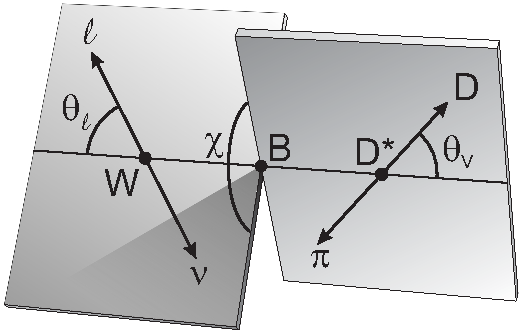
\includegraphics[width=0.65\textwidth]{./figs-theory/b_d_angular_vars.pdf}
    \caption{
        Angular variables of the $\Bzb \rightarrow D^{*+} \ellm\neulb$ decays.
        For $\Bm \rightarrow \Dz\ellm\neulb$ decays,
        only the $\theta_l$ variable exists.
    }
    \label{fig:b-d-decay-schematic}
\end{figure}

\paragraph{Leptonic current}
The leptonic currents are straightforward to evaluate,
as the weak interaction permits a perturbative calculation and the currents can
be sufficiently approximated by tree-level decays.
Evaluated in the $B$ rest frame, each lepton current of the polarization combintation
$(\lambda_W, \lambda_l)$ is a function of the lepton mass,
the invariant mass squared $q^2$ of the virtual $W$,
and $\theta_l$ as defined in \cref{fig:b-d-decay-schematic}.
The results are listed in eqs. (2.8) and (2.9) in
\cite{HAGIWARA1989569}, and are copied over with minor changes on notations:
\begin{align}
    & L^-_\pm(q^2, \theta_l) = -2 \sqrt{q^2} v d_\pm
    & L^-_0(q^2, \theta_l) &= -2 \sqrt{q^2} v d_0
    & L^-_s(q^2, \theta_l) &= 0
    \label{eqn:b-d-l-current-1} \\
    & L^+_\pm(q^2, \theta_l) = \mp \sqrt{2} m_l v d_0
    & L^+_0(q^2, \theta_l) &= \sqrt{2} m_l v(d_+ - d_-)
    & L^+_s(q^2, \theta_l) &= -2 m_l v
    \label{eqn:b-d-l-current-2}
\end{align}
where $v = \sqrt{1 - \frac{m^2_l}{q^2}}$,
$d_\pm = \frac{1 + \cos\theta_l}{\sqrt{2}}$, and $d_0 = \sin\theta_l$.

\paragraph{Hadronic current} The calculation of the hadronic currents, however,
involves non-perturbative quantum chromodynamics (QCD) effects as both the
initial and final states are mesons which are quark-anti-quark pairs bounded by
the strong interactions of QCD.
Hence, these currents are not computable in an analytical way and each of them
is re-expressed in terms of form factors (FFs),
which are a function of \qSq, instead.
These FFs are parameterized and estimated with relatively large theoretical
uncertainties with four types of methods:
use of functional properties of the matrix elements\footnote{
    Such as analyticity, unitarity, and dispersion relations.
},
heavy quark effective theory (HQET),
various quark models\footnote{
    For example QCD sum rule (QCDSR) and light cone sum rule (LCSR).
},
and lattice QCD
\cite{Bernlochner_2022}.
As mentioned in the introduction,
for \RDX ratio measurements,
the hadronic uncertainties are mostly factored out and the main importance
of the FFs lies in the precision of the lepton universality ratio predictions.
% NOTE: Check the slides for CLN vs. BGL
%   https://indico.cern.ch/event/656737/contributions/2676125/attachments/1525023/2384258/Siegen.pdf
The estimations of FFs
and the differential decay rate (which will be provided shortly after)
are often performed at a particular $q^2$ value, such as when the $D$ meson is
produced at rest in the $B$ rest frame\footnote{
    Referred to as ``zero recoil'' due to the fact that the $D$ meson is
    \emph{not recoiling} in the $B$ rest frame.
},
and are extrapolated to the full $q^2$ range by performing fits to experimental
inputs.

While not analytically calculable,
the hadronic currents are constrained by the conservation of angular momentum,
which implies that the $D$ and the virtual $W$ should have the same helicity.
For a $D^0$ meson, whose only possible helicity state is 0,
the only non-zero hadronic amplitudes are $H^0_0, H^0_s$.
For $D^*$ meson,
the amplitudes $H^+_+$ and $H^-_-$ are allowed in addition.

\paragraph{Differential decay rate}
The differential decay rate is found by first inserting
\cref{eqn:b-d-l-current-1,eqn:b-d-l-current-2}
into \cref{eqn:b-d-master-formula} then integrating over the phase space and
summing over the lepton helicities:
\begin{align}
    \frac{d\Gamma}{d q^2 d\cos\theta_l} =&
    \frac{G^2_F |V_{cb}|^2 | \vec{p}^*_D|^2 q^2}{256 \pi^3 m^2_B}
    \left(1 - \frac{m^2_l}{q^2}\right)^2 \times
    \nonumber \\
    &\bigg[
        (1 - \cos\theta_l)^2 |H_+|^2 + (1 + \cos\theta_l)^2 |H_-|^2 +
        2 \sin^2\theta_l |H_0|^2 +
    \nonumber \\
    & \frac{m^2_l}{q^2} \left(
        (\sin^2\theta_l(|H_+|^2 + |H_-|^2) + 2|H_s + H_0 \cos\theta_l|^2)
    \right)
    \bigg]
    \label{eqn:ff-ps}
\end{align}
where the \qSq dependence and the helicities of the $D$ meson in the hadronic
currents $H_{\{\pm,0,s\}}$ are omitted.

In the next sections the form factor parameterizations relevant to this analysis
for \Dz, \Dstar, and \Dstst mesons are discussed.


\subsection{Form factors in $B \rightarrow \Dz\ellm\neulb$ decays}
\label{ref:theory:ff-d0}

As discussed before,
a form factor parameterization of the hadronic currents is needed in order to
evaluate the differential decay rate.
In this analysis both \Dz and \Dstar MCs are generated with the CLN
parameterization and later reweighted offline to BGL
(more details regarding the reweighting process will be provided in
\cref{ref:mc-cor:ff}).
More details will be given for \Dz parameterizations.
For \Dstar only the parameterization schemes and parameter values will be given.

\paragraph{CLN}
For $B \rightarrow \Dz\ellm\neulb$ decays the axial vector part of the hadronic
current is vanishing due to conservation of angular momentum and parity
\cite{Bernlochner_2022}.
Each hadronic current is therefore characterized by \emph{two} FFs:
\begin{align}
    \bra{D} \bar{c} \gamma^\mu(1 - \gamma^5) b \ket{B} &=
    \bra{D} \bar{c} \gamma^\mu b \ket{B}
    \nonumber \\
    &=
    \sqrt{m_B m_D} \left[
        h_+(w)(v_B + v_D)^\mu + h_-(w)(v_B - v_D)^\mu
    \right]
    \label{eqn:b-d-cln-param}
\end{align}
where $v_i = \frac{p_i}{m_i}$,
$w(\qSq) \equiv v_B \cdot v_D = \frac{m^2_B + m^2_D - \qSq}{2 m_B m_D}$.
%%%%
In CLN parameterization \cite{Caprini_1998},
the FFs $h_+, h_-$ are re-expressed as $V_1(w), S_1(w)$:
\begin{align}
    V_1(w) &= h_+(w) - \frac{m_B - m_D}{m_B + m_D} h_-(w) \\
    S_1(w) &= h_+(w) - \frac{m_B + m_D}{m_B - m_D} \cdot \frac{w-1}{w+1} h_-(w)
\end{align}
and an expression for $V_1(w)$ is obtained by first analytically continue $w$
outside the physical region in the complex plane, then a conformal mapping
\begin{equation}
    w \rightarrow z: z =
    \frac{\sqrt{w+1} - \sqrt{2}}{\sqrt{w+1} + \sqrt{2}}
\end{equation}
is performed such that the physical region is mapped inside the unit circle of
the complex $z$-plane.
With dispersion techniques based on first principles and additional
consideration from heavy quark symmetries to further reduce number of degrees of
freedom,
$V_1(z)$ is expressed in powers of $z$, known as ``$z$-expansion'', in the
following form:
\begin{equation}
    V_1(w) = V_1(1) \cdot \left[
        1 - 8 \rho^2 z(w) + (51 \rho^2 - 10) z(w)^2 -
        (252 \rho^2 - 84) z(w)^3
    \right]
\end{equation}
where $V_1(0), \rho^2$ are FF parameters,
noting that $V_1(0)$ corresponds to the hadronic current at zero recoil.
The factor $V_1(0)$,
fitted from external data with HQET or lattice QCD constraints,
represents an overall normalization which is \emph{not cancelled} when
performing CLN to BGL reweighting but \emph{is cancelled} in subsequent fit to
\RD ratio.

The corresponding leptonic current to $S_1$ is helicity suppressed which is
proportional to the lepton mass.
Therefore this hadronic amplitude is insensitive to input data and is
constrained based on HQET:
\begin{equation}
    S_1(w) = \left\{
        1 + \Delta(-0.019 + 0.041(w - 1) - 0.015(w - 1)^2)
    \right\} V_1(w)
\end{equation}
The rest of the parameters,
namely $\rho^2, \Delta$,
are obtained from a fit to data by saturating the dispersive bounds at $1\sigma$
uncertainty \cite{Bernlochner_2022}.
The values for the parameters listed above are copied from the corresponding MC
generation code,
and are listed in \cref{tab:ff-cln-b-d}.

\begin{table}[!htb]
    \centering
    \caption{
        $B \rightarrow \Dz \ellm\neulb$ CLN FF parameterization.
    }
    \label{tab:ff-cln-b-d}
    \begin{tabular}{c|c|c}
        \toprule
        \textbf{FF parameter} & \textbf{Value} & \textbf{\Hammer name} \\
        \midrule
        $V_1(0)$ & 1.035 & \smalltt{G1}     \\
        $\rho^2$ & 1.131 & \smalltt{RhoSq}  \\
        $\Delta$ & 0.38  & \smalltt{Delta}  \\
        \bottomrule
    \end{tabular}
\end{table}

The use of CLN is criticized by the theory community because the
slope and curvature of the Isgure-Wise function,
the form factor description in the heavy quark limit,
are too closely cross-constrained by the model.
Additionally, the fit of FF normalization factors at zero recoil is not
self-consistent as the change in the slope of the form factors is not taken into
account \cite{LHCb-ANA-2020-056}.

\paragraph{BGL} Similar to CLN, the BGL parameterization
\cite{Boyd_1995,Boyd:1997kz}
is based on dispersion relations, analyticity, and crossing symmetry but
with reduced constraints,
providing more flexibility at the cost of additional
number of parameters.
The BGL parameterization is more ideal to a data-driven approach of the
determination of the FFs.

The BGL adopts the following parameterization for
$B \rightarrow \Dz\ellm\neulb$ decays:
\begin{equation}
    \bra{D} \bar{c} \gamma^\mu b \ket{B} =
    f_+ (p_B + p_D)^\mu + (f_0 - f_+) \frac{q^\mu}{q^2} (m^2_B - m^2_D)
\end{equation}
which is different than \cref{eqn:b-d-cln-param}.
Both $f_+, f_0$ are expressed as a series of $z$:
\begin{equation}
    f_{+,0}(z(w)) = \frac{1}{P_{+,0}(z(w))\phi_{+,0}(z(w))}
    \sum^\infty_{n = 0} a_{+,0}^n z(w)^n
\end{equation}
where $P_{+,0}(w)$ are known as \emph{Blaschke factors} with their expressions
listed in eq. (2.12) in \cite{Bigi_2016},
and $\phi_{+,0}$, \emph{outer functions}, are defined in eqs. (2.13) and (2.14)
of the same reference.
The $a_{+,0}$ parameters are taken from Table 4 in \cite{Bigi_2016} at $N = 2$,
which are obtained from a fit to a combination of
an unquenched lattice calculation at \emph{non-zero recoil} and experimental
data.
The $N = 2$ fit result is chosen because it is the only case that is consistent
with unitary bounds and has a non-trivial correlation matrix as reported in
Table 5 of \cite{Bigi_2016}.
The correspondence between the parameter notations used in this paper,
in Ref.~\cite{Bigi_2016}, and in \Hammer is displayed in
\cref{tab:ff-bgl-b-d}.

\begin{table}[!htb]
    \centering
    \caption{
        $B \rightarrow \Dz \ellm\neulb$ BGL FF parameterization
        notation correspondence.
    }
    \label{tab:ff-bgl-b-d}
    \begin{tabular}{c|c|c}
        \toprule
        \textbf{FF parameter} & \textbf{Ref.~\cite{Bigi_2016}} & \textbf{\Hammer name} \\
        \midrule
        $a_+^n$     & $a_n$     & \smalltt{ap}, a vector     \\
        $a_0^n$     & $b_n$\parnote{
            The $b_0$ coefficient is fixed by the other coefficients:
            $b_0 = 4.99 a_0 + 0.32 a_1 + 0.021 a_2 - 0.065 b_q - 0.004 b_2$
            due to the constraint that $f_+ = f_0$ at $\qSq = 0$.
        }
                                & \smalltt{a0}, a vector     \\
        \bottomrule
    \end{tabular}
    \begin{flushleft}
        \parnotes
    \end{flushleft}
\end{table}


\subsection{Form factors in $B \rightarrow \Dstar\ellm\neulb$ decays}
\label{ref:theory:ff-dst}

The discussions regarding CLN and BGL in \cref{ref:theory:ff-d0} also applies
here.
The CLN and BGL parameterizations of $B \rightarrow \Dstar\ellm\neulb$ will be
given first,
followed by a brief comment on calculation of \RDX.

\paragraph{CLN}
For $B \rightarrow \Dstar\ellm\neulb$ decays,
the hadronic currents are parameterized by \emph{four} FFs $V, A_{0,1,2}$:
\begin{align}
    \bra{\Dstar} \bar{c} \gamma^\mu b \ket{B}
    =\hphantom{ } &
        2i V (m_B + m_\Dstar) \varepsilon^{\mu\nu\alpha\beta}
        \epsilon^*_\nu (p_\Dstar)_\alpha (p_B)_\beta \\
    \bra{\Dstar} \bar{c} \gamma^\mu \gamma^5 b \ket{B}
    =\hphantom{ } &
        A_1 (m_B + m_\Dstar) \epsilon^{*\mu} -
        \nonumber \\
    =\hphantom{ } &
        A_2 \frac{\epsilon^* \cdot \vec{p_B} (p_B + p_\Dstar)^\mu}{m_B + m_\Dstar} +
        \nonumber \\
    =\hphantom{ } &
        2 m_\Dstar q^\mu (A_0 - A_3) \frac{\epsilon^* \cdot \vec{p_B}}{q^2}
\end{align}
in which $2 m_\Dstar A_3 = A_1(m_B + m_\Dstar) - A_2(m_B - m_\Dstar)$.
In the CLN parameterization,
these FFs are re-expressed as:
\begin{align}
    & A_1(w) = \frac{w+1}{2} r_\Dstar h_{A_1}(w)
    & A_0(w) = \frac{R_0(w)}{r_\Dstar} h_{A_1}(w)
    \label{eqn:b-dst-ff-param-1} \\
    & A_2(w) = \frac{R_2(w)}{r_\Dstar} h_{A_1}(w)
    & V(w) = \frac{R_1(w)}{r_\Dstar} h_{A_1}(w)
    \label{eqn:b-dst-ff-param-2}
\end{align}
where $r_\Dstar = 2 \frac{\sqrt{m_B m_\Dstar}}{m_B + m_\Dstar}$.
With dispersive bounds, these are expressed as:
\begin{align}
    h_{A_1}(w) &= h_{A_1}(1) \left[
        1 - 8 \rho^2 z(w) + (53 \rho^2 - 15) z(w)^2 - (231 \rho^2 - 91) z(w)^3
    \right] \\
    R_1(w) &= R_1(1) - 0.12(w-1) + 0.05(w-1)^2 \\
    R_2(w) &= R_2(1) + 0.11(w-1) - 0.06(w-1)^2 \\
    R_0(w) &= R_0(1) - 0.11(w-1) + 0.01(w-1)^2
\end{align}
The parameters used in $B \rightarrow \Dstar\ellm\neulb$ MC generation are
listed in \cref{tab:ff-cln-b-dst}.

\begin{table}[!htb]
    \centering
    \caption{
        $B \rightarrow \Dstar \ellm\neulb$ CLN FF parameterization.
    }
    \label{tab:ff-cln-b-dst}
    \begin{tabular}{c|c|c}
        \toprule
        \textbf{FF parameter} & \textbf{Value} & \textbf{\Hammer name} \\
        \midrule
        $h_{A_1}(0)$ & 0.908 & \smalltt{F1}     \\
        $\rho^2$     & 1.122 & \smalltt{RhoSq}  \\
        $R_1(1)$     & 1.270 & \smalltt{R1}  \\
        $R_2(1)$     & 0.852 & \smalltt{R2}  \\
        $R_0(1)$     & 1.15  & \smalltt{R0}  \\
        \bottomrule
    \end{tabular}
\end{table}

\paragraph{BGL}
The BGL parameterization scheme for $B \rightarrow \Dstar\ellm\neulb$ decays is
\cite{Bazavov_2021}:
\begin{align}
    \bra{\Dstar} \bar{c} \gamma^\mu b \ket{B}
    =\hphantom{ } &
        i\sqrt{m_B m_\Dstar} h_V \varepsilon^{\mu\nu\alpha\beta}
        \epsilon^*_\nu (v_\Dstar)_\alpha (v_B)_\beta \\
    \bra{\Dstar} \bar{c} \gamma^\mu \gamma^5 b \ket{B}
    =\hphantom{ } &
        \sqrt{m_B m_\Dstar} \Big[
            h_{A_1}(w+1) \epsilon^{*\mu} -
    \nonumber \\
    &\hphantom{\sqrt{m_B m_\Dstar} \Big[}
            h_{A_2} (\epsilon^* \cdot \vec{v_B}) (v_B)^\mu -
            h_{A_3} (\epsilon^* \cdot \vec{v_B}) (v_\Dstar)^\mu
        \Big]
\end{align}
with the FFs $\{h_V,h_{A_1,A_2,A_3}\}$ re-expressed as
$\{g,f,\mathcal{F}_1,\mathcal{F}_2\}$:
\begin{align}
    g(w) =& \frac{h_V(w)}{m_B \sqrt{r}} \\
    f(w) =& m_B \sqrt{r}(1 + w) h_{A_1}(w) \\
    \mathcal{F}_1 =& m^2_B \sqrt{r}(1+w)\left[
        (w - r) h_{A_1}(w) - (w - 1)(r h_{A_2}(w) + h_{A_3}(w))
    \right] \\
    \mathcal{F}_2 =& \frac{1}{\sqrt{r}} \left[
        (1+w)h_{A_1}(w) + (rw - 1) h_{A_2}(w) + (r-w)h_{A_3}(w)
    \right]
\end{align}
where $r = \frac{m_\Dstar}{m_B}$.
These FFs are proportional to $H_- - H_+, H_+ + H_-, H_0, H_s$ accordingly.
With $z$-expansion, the FFs are expanded into the form:
\begin{align}
    g(w) =& \frac{1}{P_{1^-}(z(w))\phi_g(z(w))}
        \sum^N_{n = 0} a_n z(w)^n \\
    f(w) =& \frac{1}{P_{1^+}(z(w))\phi_f(z(w))}
        \sum^N_{n = 0} b_n z(w)^n \\
    \mathcal{F}_1(w) =& \frac{1}{P_{1^+}(z(w))\phi_{\mathcal{F}_1}(z(w))}
        \sum^N_{n = 0} c_n z(w)^n \\
    \mathcal{F}_2(w) =& \frac{1}{P_{0^-}(z(w))\phi_{\mathcal{F}_2}(z(w))}
        \sum^N_{n = 0} d_n z(w)^n
\end{align}
where $P_i(z(w))$ are given in eq. (61) in \cite{Bazavov_2021}, and
$\phi_i(z(w))$ in eqs. (67--70) in the same reference.
The coefficients $\{a_n, b_n, c_n, d_n\}$ are given by a fit to unquenched
lattice calculation at non-zero recoil and data;
their values are listed in the right-most column of Table XII in the
\textbf{v1} version of \cite{Bazavov_2021}.
The parameter naming correspondence is displayed in
\cref{tab:ff-bgl-b-dst}.

\begin{table}[!htb]
    \centering
    \caption{
        $B \rightarrow \Dstar \ellm\neulb$ BGL FF parameterization
        notation correspondence.
    }
    \label{tab:ff-bgl-b-dst}
    \begin{tabular}{c|c|c}
        \toprule
        \textbf{FF parameter} & \textbf{Ref.~\cite{Bazavov_2021}} & \textbf{\Hammer name} \\
        \midrule
        $a_n$     & $a_n$     & \smalltt{avec}, a vector     \\
        $b_n$     & $b_n$     & \smalltt{bvec}, a vector     \\
        $c_n$     & $c_n$     & \smalltt{cvec}, a vector\parnote{
            The $c_n$ coefficients starts from $c_1$ instead of $c_0$.
        } \\
        $d_n$     & $d_n$     & \smalltt{dvec}, a vector\parnote{
            The $c_3$ and $d_2$ coefficients are unused in the reweighting
            based on a claim that they are not implemented in \Hammer.
            Latest version of \Hammer may have added support to these
            parameters.
        } \\
        \bottomrule
    \end{tabular}
    \begin{flushleft}
        \parnotes
    \end{flushleft}
\end{table}

\paragraph{\RDX calculation}
With FFs, the hadroic currents can be modeled based on a combination of
theoretical calculations and experimental data.
Plug these into the differential decay rate, a fully resolved
$\frac{d\Gamma}{d q^2}$ is obtained,
which can be used to compute \RDX:

\begin{equation}
    \RDX = \frac{
        \int_{m^2_\tau}^{(m_B - m_{D^{(*)}})^2} d q^2 \frac{d\Gamma}{d q^2}
    }{
        \int_{m^2_\mu}^{(m_B - m_{D^{(*)}})^2} d q^2 \frac{d\Gamma}{d q^2}
    }
\end{equation}


\subsection{Form factors in $B \rightarrow D^{**}\ellm\neulb$ decays}
\label{ref:theory:ff-dstst}

\paragraph{ISGW2}
The ISGW2 parameterization \cite{Scora_1995} is based on a
non-relavistic constituent quark model and is treated as fully predictive,
that is, without any undetermined parameter.
While historically important in providing a description of the FFs,
it is no longer considered to provide state-of-art FFs
due to its inability to improve its description with data-driven fits to
experimental data.

\paragraph{BLR}
The BLR parameterization \cite{Bernlochner_2018} provides an
model-independent FF description for four lightest ($1P$) excited \Dstst mesons
($D^*_0$, $D'_1$, $D_1$, $D^*_2$),
grouped into two heavy quark isospin doublets
$D^{1/2+}: (D^*_0, D'_1)$ and $D^{3/2+}: (D_1, D^*_2)$.
This parameterization considers all possible
$b \rightarrow c\ellm\neulb$ four-Fermi interactions and includes
$\mathcal{O}(\Lambda_\text{QCD} / m_{c,b})$ and $\mathcal{O}(\alpha_s)$
corrections
which results in FFs that can be improved by data-driven fits.
The parameterizations are listed separately in
\cref{tab:ff-blr-1-2,tab:ff-blr-3-2} for the two isospin doublets.

\begin{table}[!htb]
    \centering
    \caption{
        FF parameterization for $D^{1/2+}$ doublet $(D^*_0, D'_1)$.
    }
    \label{tab:ff-blr-1-2}
    \begin{tabular}{c|c|c}
        \toprule
        \textbf{FF parameter} & \textbf{Ref.~\cite{Bernlochner_2018}} & \textbf{\Hammer name} \\
        \midrule
        $\zeta(1)$       & 0.7     & \smalltt{zt1}     \\
        $\zeta'$         & 0.2     & \smalltt{ztp}     \\
        $\hat{\zeta}_1$  & 0.6     & \smalltt{zeta1}   \\
        \bottomrule
    \end{tabular}
\end{table}

\begin{table}[!htb]
    \centering
    \caption{
        FF parameterization for $D^{3/2+}$ doublet $(D_1, D^*_2)$.
    }
    \label{tab:ff-blr-3-2}
    \begin{tabular}{c|c|c}
        \toprule
        \textbf{FF parameter} & \textbf{Ref.~\cite{Bernlochner_2018}} & \textbf{\Hammer name} \\
        \midrule
        $\tau(1)$       & 0.7     & \smalltt{t1}     \\
        $\tau'$         & -1.6    & \smalltt{tp}     \\
        $\hat{\tau}_1$  & -0.5    & \smalltt{tau1}   \\
        $\hat{\tau}_2$  & 2.9     & \smalltt{tau2}   \\
        \bottomrule
    \end{tabular}
\end{table}

\chapter{The LHCb experiment}
\label{ref:detector}

The LHCb experiment is dedicated for $b$ and $c$-physics precision measurements.
It is one of the four large experiments
(CMS, ATLAS, ALICE, LHCb) at the Large Hadron Collider (LHC),
a superconducting circular $pp$ collider with a center of mass energy
$\sqrt{s} = 13$~TeV during its run 2 (2016--2018) operation period.

Located 100 meter underground at Franco-Swiss border,
the LHCb detector,
shown in \cref{fig:lhcb-detector},
is a forward only spectrometer covering the pseudorapidity\footnote{
    Defined as the following:
    $\eta \equiv -\ln\left[\tan\left(\frac{\theta}{2}\right)\right]$,
    with $\theta$ the angle between the 3-momentum of a particle
    and the positive direction of the beam axis.
}
range $1.9 < \eta < 4.9$.
The unusual geometry of the LHCb detector
(as opposed to $4\pi$ detectors,
for example the other three large experiments at the LHC,
with full solid angle coverage)
is largely driven by the \bbbar production mechanism at the LHC:
the dominate production mode is gluon fusion in which case the momenta of the
incoming partons are highly asymmetric in the lab frame.
As a result, the \bbbar center of mass is boosted either forward or backward
in the beam direction, as stated in \cite{Altarelli_2008}.
Simulation of \bbbar production angular distribution,
shown in \cref{fig:bbbar-prod-angular},
confirms the claim above.
With just about 4\% solid angle coverage,
the LHCb detector efficiently and economically reconstructs about 20\%
of all produced \bbbar pairs
(\cite{Belyaev_2021}).

\begin{figure}[!htb]
    \centering
    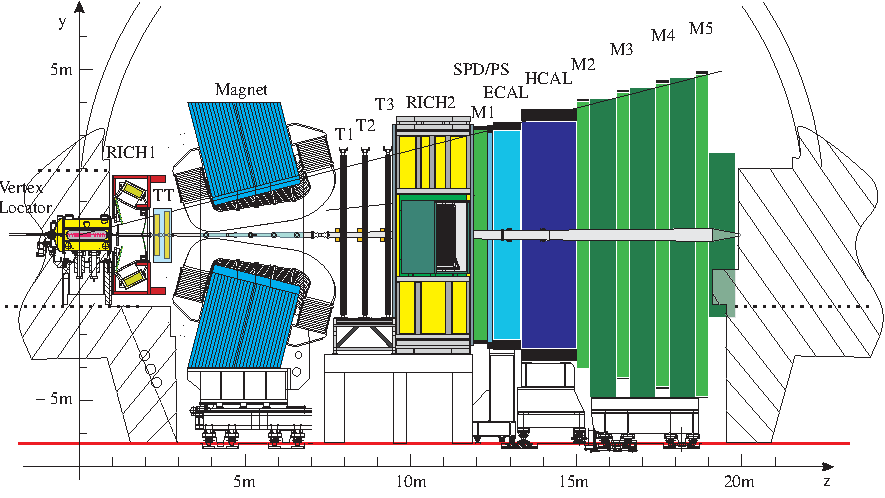
\includegraphics[width=0.95\textwidth]{./figs-detector/lhcb_detector_view.pdf}
    \caption{The LHCb detector.}
    \label{fig:lhcb-detector}
\end{figure}

\begin{figure}[!htb]
    \centering
    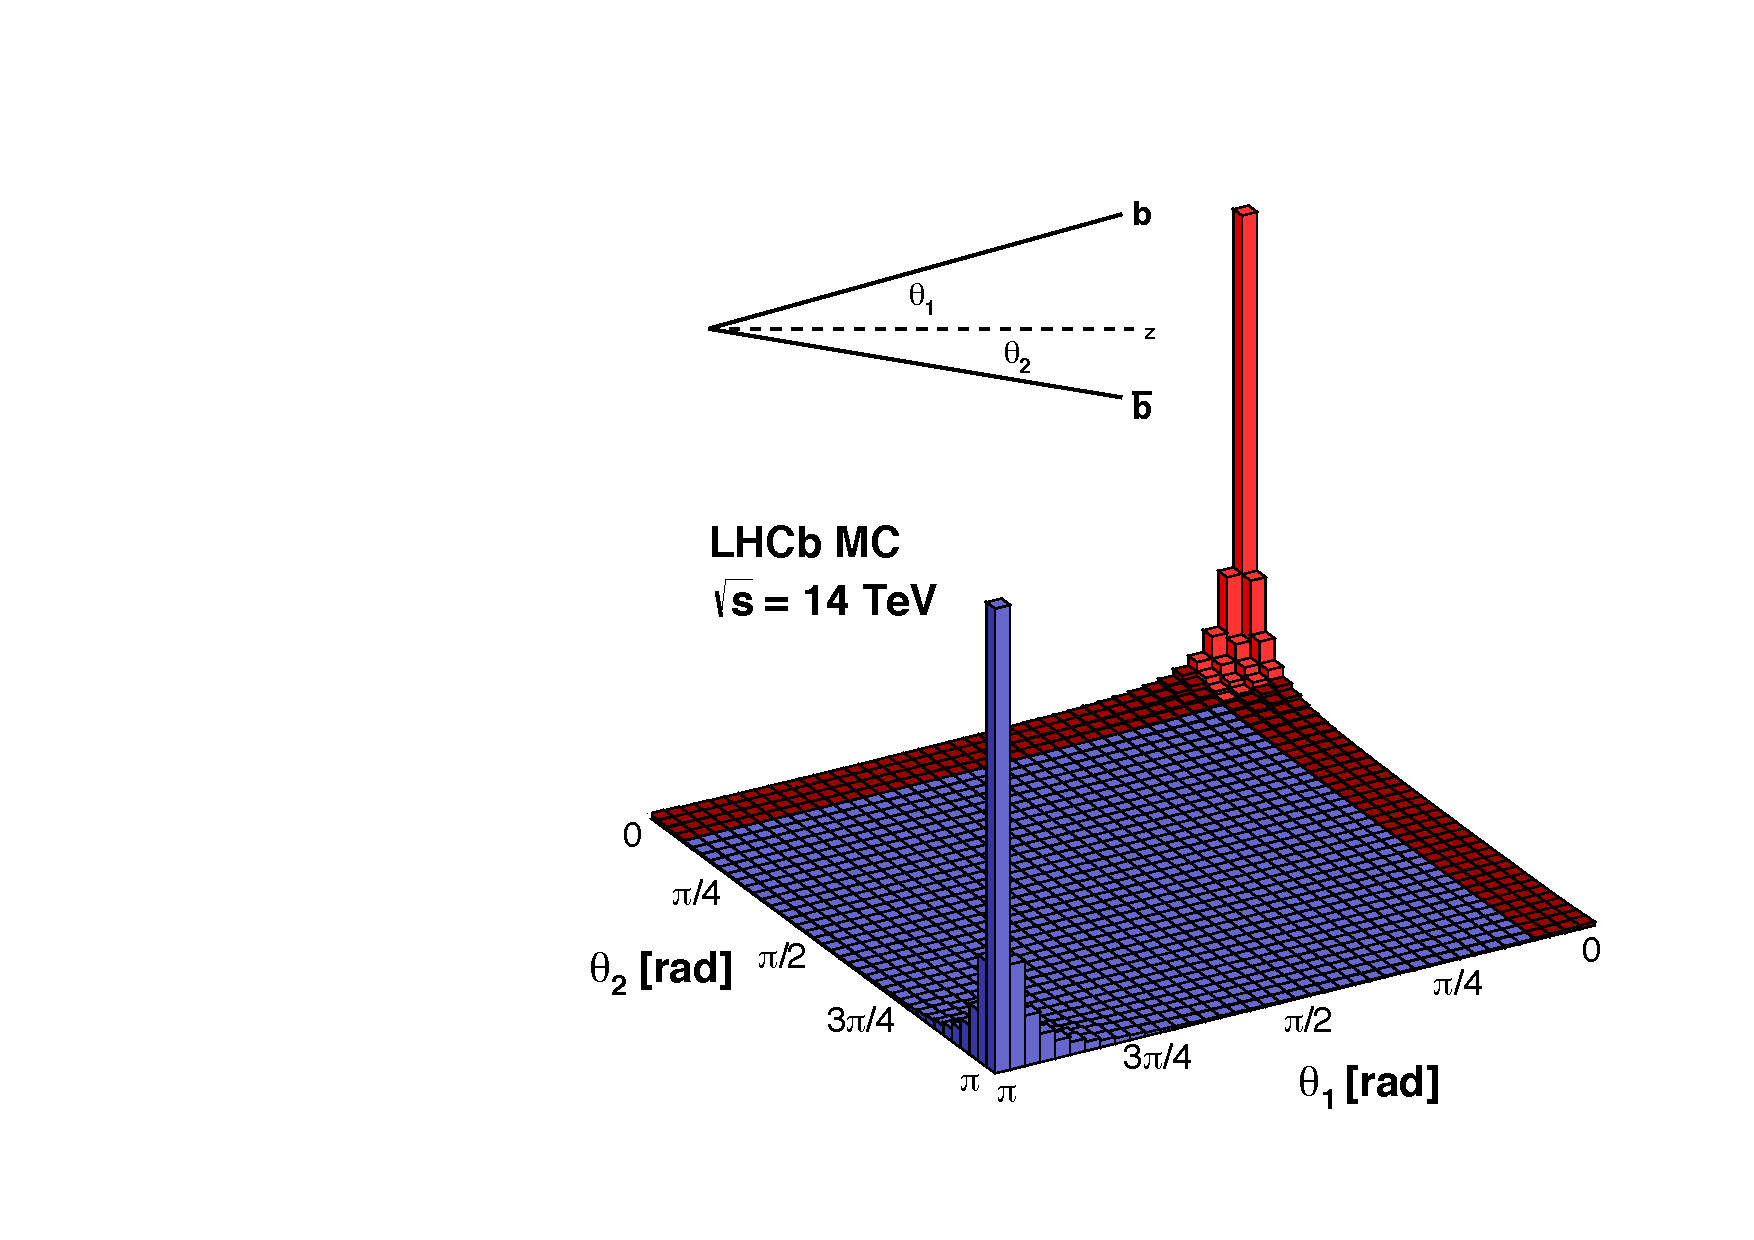
\includegraphics[width=0.6\textwidth]{./figs-detector/14_rad_acc_scheme_right.pdf}
    \caption{
        Simulated \bbbar production angular distribution at $\sqrt{s} = 14$ GeV.
        Taken from \cite{LHCb_bb_prod_angle}.
    }
    \label{fig:bbbar-prod-angular}
\end{figure}

%%%%
\chapter{Selection}
\label{ref:sel}

This chapter describes the selection procedure for samples used in this
analysis which involves an online and offline selection.
The initial online selection are a composition of
pre-defined triggers and cuts provided by the LHCb experiment;
some of them may be limiting so extra care is needed to avoid biasing important
physical quantities.
The follow-up offline selection are entirely imposed by analysts
to further balance signal selection and background rejection efficiencies
and separate the signal-like sample from various backgrounds.

Real data and MC samples used directly in the fit are selected with procedure
described in \cref{ref:sel:data,ref:sel:mc}, accordingly.
Each sample is further divided into signal-like and control background
subsamples, also known as ``skims'', with selections listed in
\cref{ref:sel:skims}.
Selection of samples used in auxiliary studies is discussed in
\cref{ref:sel:aux}.
Additional technologies are used in the selection process;
these are described in more details in
\cref{ref:sel:tech}.


\section{Data samples}
\label{ref:sel:data}

This analysis currently uses 1665~pb$^{-1}$ of proton-proton collision data
recorded by LHCb in 2016 at $\sqrt{s} = 13$~TeV.
It is planned to extend the analysis to employ data taken in the full
2016--2018 period (run 2).
The rest of the section describes selection procedures for various data samples,
which are:

\begin{itemize}
    \item \nameref{ref:sel:data:rs}:
        the nominal data samples to be fitted.
    \item \nameref{ref:sel:data:ws}:
        for characterizing various combinatorial backgrounds
        which are random combinations of the \DXmu pairs that are \emph{not}
        originating from the same $B$ decay but pass the selections
        requiring so.
    \item \nameref{ref:sel:data:fake-mu}:
        for studying the contributions from other charged particles
        mis-identified as muon in the nominal data sample.
\end{itemize}


\subsection{Right-sign samples}
\label{ref:sel:data:rs}

These are the data samples used in the fit where the signal and normalization
yields are extracted.
The samples contain right-sign \DXmu pairs,
the pairs that have the correct charges to form a legitimate $B$ meson.
That is, only \Dz\mun and \Dstarp\mun (and their charge conjugates).
The \muon in these samples are required to pass \muon particle identification
(PID) requirements.

The online selection for the \Dz\mun and \Dstarp\mun final states,
henceforth referred as \Dz channel and \Dstar channel,
are identical.
The selection involves an online trigger path:
a composition of hardware (L0) and software triggers (HLT1, HLT2),
as listed in \cref{tab:triggers}.
Overall, the online selection requires a \muon candidate to form
a well-defined vertex
with a high $p_T$ $\Dz (\rightarrow \Km \pip)$ candidate,
requiring both particles to be close to each other and are not directly coming
from the primary $pp$ decay vertex (PV).
More details about the trigger path are given below.


\begin{table}[!htb]
    \caption{
        Trigger path for this analysis.
        For terminologies such as TIS and TOS, refer to
        \cref{appx:trigger-cat}.
    }
    \label{tab:triggers}
    \centering
    \parnotereset
    \begin{tabular}{c|c}
        \toprule
        {\bf Trigger level} & {\bf Requirements} \\
        \midrule
        L0 & \Dz L0Hadron TOS || \B L0Global TIS \\
        HLT1 & \makecell{
            (\kaon~\smalltt{Hlt1TrackMVA} TOS || \pion~\smalltt{Hlt1TrackMVA} TOS)\parnote{
                This is almost equivalent to \Dz~\smalltt{Hlt1TrackMVA} TOS, with a
                $\sim\!0.0027\%$ difference in selected events in
                reconstructed data sample in \Dz channel.
                Henceforth these two trigger paths are considered equivalent.
            } || \\ \Dz~\smalltt{Hlt1TwoTrackMVA} TOS
        } \\
        HLT2 & \B~\smalltt{Hlt2XcMuXForTauB2XcMu} TOS \\
        \bottomrule
    \end{tabular}
    \begin{flushleft}
        \parnotes
    \end{flushleft}
\end{table}


%%%%
The L0 triggers are chosen to make sure events are not trigged by
the \muon track \emph{alone} which would introduce a \pt bias\footnote{
    According to table 1 in \cite{LHCb-DP-2019-001},
    the minimum \pt threshold across all L0 triggers is 1.35 GeV for 2018
    L0Muon trigger.
} on the \muon.
Such a bias is very problematic for this analysis as \muon from signal
$\tauon \rightarrow \muon \neumb \neut$ decays are typically softer and
have smaller \pt,
making signal events less likely to be selected.
A muon trigger would,
as discussed at the end of \cref{ref:detector},
actively reject signal decays as well as making the selection efficiencies for
the signal and normalization decay modes different.
%%%%
The inclusive HLT1 triggers select events containing a particle whose decay
vertex is displaced from the PV,
in this case a $\Dz \rightarrow \Km \pip$,
as described in \cite{LHCb-INT-2019-025}, Section 6.7.1.
%%%%
The \smalltt{Hlt2XcMuXForTauB2XcMu} is specifically designed for this analysis
to select \Dz\mupm candidates\footnote{
    Yes, both right-sign and wrong-signs of the \Dz\muon pairs are selected.
} with a high \pt requirement on \Dz,
while maintain minimal \pt bias on the \mupm.
%%%%
The trigger avoid cut on the invariant mass of the \Dz\muon pair
so that both the right-sign and wrong-sign samples can be selected with the same
trigger path:
the right-sign \Dz\muon pairs are more likely to form a \Dstar meson,
producing a peak around the mass of \Dstar,
whereas the wrong-sign \Dz\muon pairs are dominated by random combinations thus
not peaking.
The cuts imposed by the HLT2 line are listed in \cref{tab:cut-hlt2}.


\begin{table}[!htb]
    \caption{Cuts defined in \smalltt{Hlt2XcMuXForTauB2XcMu}.}
    \label{tab:cut-hlt2}
    \centering
    \begin{tabular}{ c | rll}
        \toprule
        {\bf Particle} & {\bf Variable}               & {\bf Cuts}               \\
        \midrule
        \kaon, \pion   & \pt                          & $> 200$ MeV              \\
                       & Max \pt                      & $> 800$ MeV              \\
                       & \ptot                        & $> 5$ GeV                \\
                       & \ipChiSq                     & $> 9$                    \\
                       & \PID{$K$}                    & $> 2\;(K)$, $< 4\;(\pi)$ \\
        \midrule
        \Dz            & \pt                          & $> 2000$ MeV             \\
                       & $|\pi\;\pt|+|K\;\pt|$        & $> 2.5$ GeV              \\
                       & $m$                          & 1830--1910 MeV           \\
                       & \anyChiSq{vertex}/ndf        & $< 10$                   \\
                       & \anyChiSq{FD}                & $> 25$                   \\
                       & \DIRA                        & $> 0.999$                \\
                       & Child pair \DOCA             & $< 0.1$ mm               \\

        \midrule
        \muon          & \ipChiSq                     & $> 16$                   \\

        \midrule
        \Dz\muon       & \anyChiSq{vertex}/ndf        & $< 15$                   \\
                       & \anyChiSq{FD}                & $> 50$                   \\
                       & \DIRA                        & $> 0.999$                \\
                       & \DOCA                        & $< 0.5$ mm               \\
        \bottomrule
    \end{tabular}
\end{table}


Additional offline selections with stricter vertex quality and PID requirements
are applied to both \Dz and \Dstar channels.
%%%%
Furthermore, only the right-sign $D^{(*)}\mu$ candidates are kept.
%%%%
The offline selections that are shared among \Dz and \Dstar channels are listed
in \cref{tab:cut-stripping,tab:offline-cut-common}.
The additional \Dz only cuts are listed in \cref{tab:offline-cut-d0},
the \Dstar in \cref{tab:offline-cut-dst}.

Due to the fact that the \Dz and \Dstar channel have the same online selection,
some events will appear in both,
making the two channels correlated.
%%%%
This correlation is removed by a \Dstar veto procedure in the \Dz channel,
and is discussed in \cref{ref:sel:tech:veto}.

Previous analyses (\cite{PhysRevLett.115.111803,LHCb-ANA-2020-056})
showed that a tighter \muon PID reduces other charged species misidentified
(misID) as \muon, reducing the systematic uncertainty due to misID effects.
However, the standard LHCb \muon PID has low efficiency at low \pt.
Therefore, an offline \muon PID method, termed \UBDT, is developed to reduce
misID while maintain a flat \pt response.
A brief overview on this method is provided in \cref{ref:sel:tech:ubdt}.


\begin{table}[!htb]
    \caption{Base offline selections (stripping) for both \Dz and \Dstar channels.}
    \label{tab:cut-stripping}
    \centering
    \begin{tabular}{c|rll}
        \toprule
        {\bf Event-Level }      & {\bf Variable}               & {\bf Cuts}               \\
        \midrule
        GEC                     & nSPDhits                     & $< 600$                  \\
        PV cut                  & nPV                          & $\geq1$                  \\
        \toprule
        {\bf Particle }         & {\bf Variable}               & {\bf Cuts}               \\
        \midrule
        $K, \pi$                & \pt                          & $> 300$ MeV              \\
                                & \ptot                        & $> 2$ GeV                \\
                                & \anyChiSq{IP}                & $> 9$                    \\
                                & \isMuon                      & \texttt{False}           \\
                                & \PID{$K$}                    & $> 4\;(K)$, $< 2\;(\pi)$ \\
                                & GhostProb                    & $< 0.5$                  \\
        \midrule
        \Dz                     & $|\pi\;\pt|+|K\;\pt|$        & $> 2.5$ GeV              \\
                                & $m - m_\text{PDG}$           & $< 80$ MeV               \\
                                & \anyChiSq{vertex}/nof        & $< 4$                    \\
                                & \anyChiSq{FD}                & $> 25$                   \\
                                & \DIRA                        & $> 0.999$                \\
        \midrule
        \muon                   & \ptot                        & $> 3$ GeV               \\
                                & \ipChiSq                     & $> 16$                  \\
                                & isMuon                       & \texttt{True}           \\
                                & \PID{$\mu$}                  & $> -200$                \\
                                & GhostProb                    & $< 0.5$                 \\
        \midrule
        \Dz\muon                & $m$                          & 0--10 GeV               \\
                                & \anyChiSq{vertex}/ndf        & $< 6$                   \\
                                & \DIRA                        & $>0.999$                \\
        \bottomrule
    \end{tabular}
\end{table}


\begin{table}[!htb]
    \caption{Additional offline selections shared among \Dz and \Dstar channels.}
    \label{tab:offline-cut-common}
    \centering
    \begin{tabular}{c|rll}
        \toprule
        {\bf Event-Level }  & {\bf Variable}               & {\bf Cuts}               \\
        \midrule
        GEC                 & nSPDhits                     & $< 450$\parnote{
            This is to reduce correlation for \emph{TIS and TOS} candidates to make
            trigger emulation more robust.
            See \cref{ref:mc-emulation:correlation-tos-tis} for more details.
        }                                                                             \\
        \toprule
        {\bf Particle}      & {\bf Variable}               & {\bf Cuts}               \\
        \midrule
        $K, \pi$            & \pt                          & $> 500$ MeV              \\
                            & HLT1 TOS track \pt           & $> 1.7$ GeV              \\
                            & \ptot                        & $< 200$ GeV\parnote{
                                This is to make \ptot consistent with extended
                                \pidcalib binning.
                            }                                                         \\
                            & \anyChiSq{IP}                & $> 45$                   \\
                            & \isMuon                      & \texttt{False}           \\
                            & \PID{$K$}                    & $> 4\;(K)$, $< 2\;(\pi)$ \\
                            & GhostProb                    & $< 0.5$                  \\
        \midrule
        \Dz                 & \pt                          & $> 2$ GeV                \\
                            & $|\pi\;\pt|+|K\;\pt|$        & $> 1.4$ GeV              \\
                            & $\log(\IP)$\parnote{
                                \IP in terms of the \PrmVtx.
                                That is, the reconstructed \Dz is inconsistent
                                of coming from \PrmVtx directly.
                            }                              & $> -3.5$                 \\
                            & \anyChiSq{IP}                & $> 9$                    \\
                            & \anyChiSq{vertex}/ndf        & $< 4$                    \\
                            & \anyChiSq{FD}                & $> 250$                  \\
                            & \DIRA                        & $> 0.9998$               \\
        \midrule
        \muon               & \ptot                        & 3-100 GeV                \\
                            & $\log_{10}(1 - \vec{p}_\mu \cdot \vec{p}_i / (|p_\mu||p_i|))$,
                              $i \in \{K, \pi\}$
                                                           & $> -6.5$                 \\
                            & $\eta$                       & 1.7--5                   \\
                            & \ipChiSq                     & $> 45$                   \\
                            & GhostProb                    & $< 0.5$                  \\
                            & \PID{$\mu$}                  & $> 2$                    \\
                            & \PID{$e$}                    & $< 1$                    \\
                            & \UBDT\parnote{
                                This is a BDT-based \muon PID algorithm,
                                which is discussed in \cref{ref:sel:tech:ubdt}.
                            }
                                                           & $> 0.25$                 \\
        \bottomrule
    \end{tabular}
    \begin{flushleft}
        \parnotes
    \end{flushleft}
\end{table}


\begin{table}[!htb]
    \caption{Offline cuts exclusive to \Dz channel.}
    \label{tab:offline-cut-d0}
    \centering
    \begin{tabular}{c|rll}
        \toprule
        {\bf Particle}  & {\bf Variable}               & {\bf Cuts}      \\
        \midrule
        \Dz\muon        & $m$                          & $< 5200$ MeV\parnote{
            The odd-looking 5200 is to avoid a peak around 5280 due to misID
            in \Bm mass spectrum.
            For \Bzb, the misID peak around 5280 is insignificant, so the cut
            is placed at 5280, at which value the neutrino is produced
            \emph{at rest in $B$ frame}, which covers a small phase space.
        }    \\
                        & {\footnotesize$\begin{aligned}
                                \text{Max}(
                                    &|\Delta m_\text{veto,1} - 145.454|, \\
                                    &|\Delta m_\text{veto,2} - 145.454|
                                )
                           \end{aligned}$}\parnote{
                            \label{parnote:dst-veto}
                            To reduce overlapping events between
                            \Dz and \Dstar channels.
                            Discussed in \cref{ref:sel:tech:veto}.
                        }                              & $> 4$ MeV       \\
                        & $\Delta m_\text{alt hypo}$\parnoteref{parnote:dst-veto}
                                                       & $> 165$ MeV     \\
                        & transverse flight distance   & $< 7$ mm        \\
                        & \anyChiSq{vertex}/ndf        & $< 6$           \\
                        & \DIRA                        & $> 0.9995$      \\
        \bottomrule
    \end{tabular}
    \begin{flushleft}
        \parnotes
    \end{flushleft}
\end{table}


\begin{table}[!htb]
    \caption{Offline cuts exclusive to \Dstar channel.}
    \label{tab:offline-cut-dst}
    \centering
    \begin{tabular}{c|rll}
        \toprule
        {\bf Particle}  & {\bf Variable}                 & {\bf Cuts}    \\
        \midrule
        slow \pion     & GhostProb                       & $< 0.25$      \\
        \midrule
        \Dstarp        & $|m - m_\Dz - 145.454|$\parnote{
                           This is to require $m_\Dstarp$ to close to
                           its reference (PDG) mass,
                           up to a reconstruction effect on
                           $m_\Dz$.
                       }                                 & $< 2$ MeV     \\
                       & \anyChiSq{vertex}/ndf           & $< 10$        \\
        \midrule
        \Dz\muon       & \anyChiSq{vertex}/ndf           & $< 6$         \\
                       & \DIRA                           & $> 0.999$     \\
        \midrule
        \Dstarp\muon   & $m$                             & $< 5280$ MeV  \\
                       & transverse flight distance      & $< 7$ mm      \\
                       & \anyChiSq{vertex}/ndf           & $< 6$         \\
                       & \anyChiSq{vertex}               & $< 24$        \\
                       & \DIRA                           & $> 0.9995$    \\
        \bottomrule
    \end{tabular}
    \begin{flushleft}
        \parnotes
    \end{flushleft}
\end{table}


\subsection{Wrong-sign samples}
\label{ref:sel:data:ws}

The wrong sign samples are used to model various combinatorial backgrounds.
For the \Dz channel,
the \Dz\mup pairs are almost exclusively of combinatorial nature\footnote{
    The right-sign sample are reconstructed as the following decay:
    $\Bm \rightarrow \Dz (\rightarrow \Km \pip) \mun$,
    so \Dz\mup pairs are unphysical at tree level thus are most likely
    resulting from random combinations.
}
and is the only dominant combinatorial background;
this is referred as \BComb.
For the \Dstar channel,
a \Dstarp may randomly combine with a \emph{wrong-sign \mup} (\BComb);
alternatively, a \Dz may combine with a \emph{wrong-sign slow \pim} to form a
\Dstarm (\DstComb).
The modeling of these backgrounds will be discussed in
\cref{ref:fit:tmpl:comb}.

The online selection for wrong-sign samples are the same as the right-sign,
as described in \cref{ref:sel:data:rs}.
The offline selection is also mostly identical, with a few differences listed
below:

\begin{itemize}
    \item \Dz channel, wrong-sign \muon (\BComb):
        The wrong-sign \Dz\mup candidates are used in place of the right-sign
        \Dz\mun.
    \item \Dstar channel, wrong-sign \muon (\BComb):
        The wrong-sign \Dz\mup candidates are used.
    \item \Dstar channel, wrong-sign \pion (\DstComb):
        The right-sign \Dz\mun candidates are used,
        but a wrong-sign slow \pim is selected so the \Dz\pim pair
        forms a wrong-sign \Dstarm.
\end{itemize}


\subsection{Fake muon samples}
\label{ref:sel:data:fake-mu}

The fake \muon samples,
labeled as ``misID samples'',
are used to estimate the contribution from events where
the \muon candidate is in fact a particle of a different species.
Such mis-identifications happen in both right-sign and wrong-sign nominal
samples thus the fake muon samples similarly contain two components:
both right-sign and wrong-sign misID samples share the same selections
as the respective nominal sample,
except for \muon PID which is replaced by an explicit \muon veto
(not \isMuon).
Also, only 10\% of event passing the fake \muon online selection are stored to
save storage space.
The contribution due to \muon misID will be studied in
\cref{ref:fit:tmpl:misid}.

\section{MC simulation}
\label{ref:sel:mc}

A large number of MC simulation samples is used to
model the signal, normalization, and partially reconstructed backgrounds in
data.
To reduce simulation time, tracker-only (TO) MC, which has all but the tracking
system of the detector turned off (set to passive material), are used.
Additional small full simulation (FullSim) samples are produced for year 2016 to
aid emulations of the missing detector responses (mainly for trigger).
The emulation procedures are discussed in \cref{ref:mc-emulation}.

MC samples used for both \Dz and \Dstar channels are listed in
\cref{tab:mc-d0-dst}, with TO and FullSim numbers listed separately.
Some samples contribute to both channels due to feed down\footnote{
    This means that the selection procedure was unable to find the
    additional slow \pion required to reconstruct a \Dstar, thus only a
    \Dz was constructed and the candidate is \emph{feed down} from \Dstar
    channel to \Dz channel.
}, and are indicated in the same table.

Both TO and FullSim MC samples are loosely filtered to keep events in LHCb
acceptance, with filtering cuts, mostly to save storage space,
listed in \cref{tab:gen-cut}.
%%%%
The online and offline selection are aligned with that of right sign real \muon
sample,
with the understanding that trigger and PID responses are emulated offline and
applied as weights (for L0 trigger and PID) and cuts
(for HLT1 and HLT2 trigger).
%%%%
Additional truth level requirements\footnote{
    For MC samples, each reconstructed particle is associated with a true
    particle ID. The truth level requirements (truth-matching) demands that
    the true ID is the same as specified in the simulation.
    For example, for a candidate from  MC $\Bm \rightarrow \Dz\mun$ decay,
    the reconstructed \muon is required to have a true ID of a MC true \muon.
} are placed to ensure the selected decay
chain is compatible with simulation specification.
This effectively removes ghost and misidentified tracks, providing a consistent
modelling and ensuring orthogonality between MC samples.

\begin{table}
    \caption{List of MC filtering cuts at generator level.}
    \label{tab:gen-cut}
    \centering
    \begin{tabular}{c|rll}
        \toprule
        {\bf Particle}  & {\bf Variable}               & {\bf Cuts}      \\
        \midrule
        \kaon, \pion    & $p_x / p_z$                  & -0.38--0.38     \\
                        & $p_y / p_z$                  & -0.28--0.28     \\
                        & $\theta$                     & $> 0.01$~rad    \\
                        & \pt                          & $> 250$~MeV     \\
        \midrule
        \muon           & $p_x / p_z$                  & -0.38--0.38     \\
                        & $p_y / p_z$                  & -0.28--0.28     \\
                        & $\theta$                     & $> 0.01$~rad    \\
                        & \ptot                        & $> 2950$~MeV    \\
        \midrule
        \Dz             & \pt                          & $> 15$~GeV      \\
                        & \ptot                        & $> 2450$~MeV    \\
        \bottomrule
    \end{tabular}
\end{table}

The heavy $D^{**}$ and $DDX$ MC are cocktails, with the same compositions as
listed in \cite{LHCb-ANA-2020-056}.
The heavy $D^{**}$ MC suffer from the problem that the $\piz \piz$ decays
are not simulated, inconsistent of the isospin limit.
The missing $\piz \piz$ contribution is modelled by randomly selecting $\frac{1}
{3}$ of $\pip \pim$ candidates and treating them as \emph{isolated} regardless
of their isolation BDT scores.
The isolation BDT, briefly discussed in \cref{ref:sel:tech:iso-bdt},
is used to estimate the probability of unused nearby charged tracks to originate
from the same $\D^{(*)}\mu$ vertex.

\section{Signal (ISO) and control background (1OS, 2OS, DD) skims and the isolation BDT}
\label{ref:sel:skims}

The signal and control skims (sub-samples) are separated by inspecting if there
are additional charged tracks in the event that are likely originating from the
same decay vertex (typically a $B$ decay vertex, and will be referred as so in
later text) as the reconstructed \DXmu pair;
if there is no such track,
the \DXmu pair is considered \emph{isolated} and is placed in the signal skim;
otherwise it is categorized as one of the control skims.

\paragraph{The isolation BDT}
A multivariate BDT,
referred as the ``isolation BDT'',
conceptually identical to the one used in \cite{LHCb-ANA-2020-056},
is trained on LHCb run 2 simulation
with training variables listed in \cref{tab:iso-bdt-input}
to provide a score-based estimation on if a charged track is originating from
the \B (\DXmu) vertex or not.


\begin{table}[!htb]
    \centering
    \caption{Training variables for the isolation BDT.}
    \label{tab:iso-bdt-input}

    % FIXME: Confirm these w/ Phoebe
    \begin{tabularx}{0.8\linewidth}{r|X}
        \toprule
        \textbf{Variable} & \textbf{Comment} \\
        \midrule
        PV \ipChiSq &
        Increase in the $\chi^2$ of the primary $pp$ vertex (PV) fit if the
        track is included.
        Higher $\chi^2$ implies that the track is less likely to coming from the
        fitted vertex.
        \\
        %%%%
        SV \ipChiSq &
        Increase in the $\chi^2$ of the secondary $D^{(*)}$ vertex (SV) fit if
        the track is included. \\
        %%%%
        track \pt & - \\
        track opening &
        The cosine of the angle between the track and the flight direction
        of the \DXmu pair.
        \\ %%%%
        \midrule
        \anyChiSq{FD} &
        The significance of the flight distance fit with this track included. \\
        %%%%
        $\Delta\anyChiSq{FD}$ &
        The difference in \anyChiSq{FD} with and without the track included. \\
        \bottomrule
    \end{tabularx}
\end{table}


The isolation BDT is applied on all charged long tracks in the event,
providing isolation scores for each of them where higher score implies higher
probability of coming from the \B vertex,
referred to as ``anti-isolated''.
Three tracks with highest isolation scores
(the ones that are most likely to be anti-isolated)
are saved in descending order\footnote{
    So the first one is the most anti-isolated one among all charged tracks
    in the event.
}.


Below a brief description for the signal sample and the main physics background
control samples is provided.
The dominate decay mode for each skim is also listed; these skims still contain
a composition of many decay modes.
The actual isolation selections are listed in \cref{tab:skim-cut}.

\begin{itemize}
    \item ISO: $B \rightarrow D^{(*)} \lepton \neulb$, with $\lepton \in \{\muon,
        \tauon\}$.
        This is referred as signal, or ``isolated'', sample.
        It requires that no additional charged track is from the \B vertex
        (in a probabilistic sense, with probability related to the isolation
        score)
        and is compatible with a fully reconstructed \B decay
        (ignoring missing neutrino(s)).
        % TODO: Maybe list yield, and compare to run 1, and include figures?

    \item 1OS: $B \rightarrow D^{**} \lepton \neulb$.
        This control sample, enriched in excited charm states,
        requires one and only one additional anti-isolated charged long track
        that is compatible with a \pion PID hypothesis and has correct charge
        for a $D^{**} \rightarrow D^{(*+)}\pim$ decay.

    \item 2OS: $B \rightarrow D^{**}_H \lepton \neulb$,
        where $H$ stands for ``heavy''.
        This control sample is enriched in highly excited (heavy) charm states,
        which is selected by requiring two and only two anti-isolated \pion-like
        long tracks of opposite charge,
        capable of $D^{**}_H \rightarrow D^{(*)} \pip\pim$ decay.

        % Why?
        This sample also provides an independent selection of
        $B \rightarrow D^{(*)}D X$ backgrounds, where the \pip\pim fit into the
        $X$ category and \kaon escapes isolation detection.

    \item DD: $B \rightarrow D^{(*)}D X$,
        with dominate $D \rightarrow \Kp \mun \neumb X$ sub-decays.
        This is a double-charm ($DD$) control sample,
        which is selected by requiring at least one anti-isolated track,
        a \kaon-like long track\footnote{
            This means the track went through both upstream and downstream
            trackers, and is generally of good tracking quality.
        } and a hard track in the three most anti-isolated tracks\footnote{
            Note that these three requirements can be satisfied by a single
            track.
        }.
\end{itemize}


\begin{table}[!htb]
    \caption{Signal and control sample isolation requirements.}
    \label{tab:skim-cut}
    \centering
    \begin{tabular}{c|rll}
        \toprule
        {\bf Sample}  & {\bf Variable}              & {\bf Cuts}     \\
        \midrule
        ISO           & \isoBDT{1}                  & $< 0.15$       \\
        \midrule
        1OS           & \isoBDT{1}                  & $> 0.15$       \\
                      & \isoBDT{2}                  & $< 0.15$       \\
                      & \isoTrack{1}                & $= 3$\parnote{
                          This means a long track.
                      }                                              \\
                      & $p_1$                       & $> 5$ GeV      \\
                      & $p_{T,1}$                   & $> 0.15$ GeV   \\
                      & \ProbNN{$K_1$}              & $< 0.2$        \\
                      & $Q_1 \cdot \text{PID}_\Dz$\parnote{
                          Apply to \Dz channel,
                          which implies that the anti-isolated \pip can
                          form a \Dstarp with the \Dz.
                      }                             & $> 0$          \\
                      & $Q_1 \cdot \text{PID}_\Dstar$\parnote{
                          Apply to \Dstar channel.
                          Here it is required that the anti-isolated \pim can
                          form a $D^{**0}$ with the \Dstarp.
                      }                             & $< 0$          \\
        \midrule
        2OS           & \isoBDT{1}                  & $> 0.15$       \\
                      & \isoBDT{2}                  & $> 0.15$       \\
                      & \isoBDT{3}                  & $< 0.15$       \\
                      & \isoTrack{1}                & $= 3$          \\
                      & \isoTrack{2}                & $= 3$          \\
                      & {\footnotesize
                         Max$(p_1 \cdot (p_{T,1} > 0.15 \text{ GeV}),
                              p_2 \cdot (p_{T,2} > 0.15 \text{ GeV}))$
                        }
                                                    & $> 5$ GeV      \\
                      & \ProbNN{$K_1$}              & $< 0.2$        \\
                      & \ProbNN{$K_2$}              & $< 0.2$        \\
                      & $Q_1 \cdot Q_2$             & $< 0$          \\
        \midrule
        DD            & \isoBDT{1}                  & $> 0.15$       \\
                      & {\footnotesize$\begin{aligned}
                            \text{Max}(
                            &p_1 \cdot (p_{T,1} > 0.15\text{ GeV}),  \\
                            &p_2 \cdot (p_{T,2} > 0.15\text{ GeV})
                                 \cdot (\text{\isoBDT{2}} > -1.1),   \\
                            &p_3 \cdot (p_{T,3} > 0.15\text{ GeV})
                                 \cdot (\text{\isoBDT{3}} > -1.1)
                            )
                        \end{aligned}$}             & $> 5$ GeV      \\
                      & Max(\ProbNN{$K_{1,2,3}$})   & $> 0.2$        \\
                      & \isoTrack{\text{the one passing $K$ PID requirement}}
                                                    & $= 3$          \\
                      & \isoBDT{\text{the one passing $K$ PID requirement}}
                                                    & $> -1.1$       \\
        \bottomrule
    \end{tabular}
    \begin{flushleft}
        \parnotes
    \end{flushleft}
\end{table}

\section{Auxiliary samples}
\label{ref:sel:aux}

A $\Bp \rightarrow \jpsi \Kp$ sample is used to derive $B$ kinematic and
multiplicity corrections\footnote{
    The correction procedure is described in \cref{ref:mc-cor:init:jpsi-k}.
} to MC samples.
The data sample is selected from \mup\mun\Kp final states, with the \mup\mun
pair at \jpsi resonance,
and the invariant mass of the 3-particle final state around the reference mass
of \Bp.
The offline selection cuts for $\jpsi\Kp$ are listed in
\cref{tab:cut-jpsik}.
The MC sample used to compare with $\jpsi \Kp$ data is selected with the same
procedure, with PID cuts applied as weights\footnote{
    The weights are obtained from \pidcalib, with a method similar to that in
    \cref{ref:mc-emulation:pid}).

    An extended PID binning range is chosen to cover as much phase space of
    \kaon and \muon as possible.
    There may still be events outside the covering region, in which case the PID
    weights from nearby bin is applied,
    to avoid explicit cuts on the \jpsi\kaon data control sample.
}.
The number of MC events after filtering\footnote{
    This is also referred as ``event on disk''.
} is listed in \cref{tab:add-mc-samples}.

\begin{table}[htb]
    \caption{Offline cuts on $\jpsi K$ samples.}
    \label{tab:cut-jpsik}
    \centering
    \begin{tabular}{ c | rll}
        \toprule
        {\bf Particle}    & {\bf Variable}               & {\bf Cuts}               \\
        \midrule
        \kaon             & \pt                          & $> 500$ MeV              \\
                          & \PID{$K$}                    & $> 4$                    \\
        \midrule
        \mun, \mup        & \pt                          & $> 500$ MeV              \\
                          & \ipChiSq                     & $> 4$                    \\
                          & \PID{\muon}                  & $> 2$                    \\
        \midrule
        \mun\mup (\jpsi)  & $m_\text{mea}$\parnote{
            $m_\text{mea}$ refers to measured mass, which is the invariant
            mass given by the sum of daughters' four momenta,
            without any topological constraint.
            On the other hand, $m$ is given by a vertex fit,
            which is typically of better quality.
        }                                                & 3060--3140 MeV           \\
                          & \anyChiSq{FD}                & $> 25$                   \\
        \midrule
        \Bp               & $m$                          & 5150--5350 MeV           \\
                          & \anyChiSq{vertex}            & $< 18$                   \\
                          & \ipChiSq                     & $< 12$                   \\
                          & \DIRA                        & $> 0.9995$               \\
        \bottomrule
    \end{tabular}
    \begin{flushleft}
        \parnotes
    \end{flushleft}
\end{table}

A simulated $\Dz \rightarrow \Km \pip$ MC sample,
also listed in \cref{tab:add-mc-samples},
is requested to model the momentum smearing in the misID sample due to
$K, \pi$ decay-in-flight into an authentic \muon,
which is described in \cref{ref:fit:tmpl:misid:dif}.

\begin{table}[htb]
    \caption{
        Additional MC control samples.
        All samples are full simulations.
    }
    \label{tab:add-mc-samples}
    \centering
    \parnotereset
    \begin{tabular}{l|c|c|c}
        \toprule
        \makecell{\centering\bf MC ID} & {\bf Decay mode} & {\bf Sim08}\parnote{
            This is a mixture of Sim08e (\pythia{6}, \pythia{8})
            and Sim08i (\pythia{8}).
        } & {\bf Sim09k} \\
        \midrule
        22162000\parnote{
            Currently the 2012 MC are still used for this analysis.
            It is planned to update to a run 2 MC at a future time.
        } & $\Dz \rightarrow K \pi$ & 3M & -- \\
            12143001 & $\Bp \rightarrow \jpsi \Kp$ & -- & 4M \\
        \bottomrule
    \end{tabular}
    \begin{flushleft}
        \parnotes
    \end{flushleft}
\end{table}

\section{Additional technologies used in selection}
\label{ref:sel:tech}


\subsection{Isolation BDT}
\label{ref:sel:tech:iso-bdt}


\subsection{Veto of overlapping candidates}
\label{ref:sel:tech:veto}

% See this note: https://github.com/umd-lhcb/rdx-run2-analysis/blob/master/docs/cuts/Dst_veto_in_D0.md
% TODO: The number need to be updated
Since the selection of a \Dstar\muon pair always requires the existence
of a \Dz\muon pair,
there is about 35\% of events in the signal sample\footnote{
    Defined in \cref{ref:sel:data:iso}.
} of the \Dstar channel leaks into \Dz channel.
This is likely due to the fact that slow \pion typically has poor tracking
resolution (small \ipChiSq), making the \Dz\pion vertex of poor quality which
makes the reconstruction fail and \Dstar partially reconstructed as \Dz.
To make \Dstar and \Dz channel more orthgonoal

To veto the overlapping candidates between \Dz and \Dstar channel,
a tool\footnote{
    Named \texttt{TupleToolApplyIsolationVetoDst}, which can be found at
    \techurllink{https://github.com/umd-lhcb/TupleToolSemiLeptonic/blob/master/Phys/TupleToolSemiLeptonic/src/TupleToolApplyIsolationVetoDst.cpp}{github/umd-lhcb/TupleToolSemiLeptonic}
}.
is added to the \davinci reconstruction sequence, which processes all tracks
in the event with the following procedure:

\begin{enumerate}
    \item Denote the track as $t$
    \item Refit a vertex from \Dz and $t$.
    \item Compute $\Delta m_\text{veto} \equiv m_{\Dz t} - m_\Dz$
    \item Test if $\Delta m_\text{veto} \in [140~\text{GeV}, 160~\text{GeV}]$.
        If it is, record $\Delta m_\text{veto}$ and the isolation BDT
        score of this track.
\end{enumerate}

From all recorded BDT scores and $\Delta m_\text{veto}$, the
$\Delta m_\text{veto}$ of the tracks with top two BDT scores are saved.
It is then filtered offline (listed in \cref{tab:offline-cut-d0})
that these two tracks,
the best slow \pion candidates,
are \emph{incompatible} with
forming a \Dz\pion vertex with a mass close to \Dstar PDG mass.

Note that this tool does not rank tracks based \emph{solely} on the isolation,
because the poor tracking resolution of the slow \pion implies that the track is
\emph{not guaranteed} to have a large isolation score, as it maybe more
compatible to be originating from PV, instead of the \B vertex.
Ranking tracks that fall within the $[140~\text{GeV}, 160~\text{GeV}]$
mass window based on their BDT scores
makes the veto procedure more robust, as reported in \cite{LHCb-ANA-2020-056}.

In addition, an alternative mass hypothesis is tested
(offline, also listed in \cref{tab:offline-cut-d0}), where the reconstructed
\muon is treated as a \pion,
and $\Delta m_\text{alt hypo} = m_{\Dz\muon_\text{as \pion}} - m_\Dz$
is computed\footnote{
    By using the 3-momentum of the \muon, while using $m_\pion$ as the invariant
    mass of the track.
} and required to be inconsistent with \Dstar PDG mass.

The veto procedures are applied on all samples of the \Dz channel only.


\subsection{Muon PID}
\label{ref:sel:tech:ubdt}

To maintain minimum bias on \muon \pt, a multivariate BDT,
referred as \UBDT, using uBDT method in TMVA class,
is trained to reject misidentified \muon while keeping rejection
efficiency flat on \pt,
as described in \cite{LHCb-ANA-2020-056}.

The \UBDT has been re-trained on LHCb run 2 MC\footnote{
    The updated project can be found at
    \techurllink{https://github.com/umd-lhcb/MuonBDTPid}{github/umd-lhcb/MuonBDTPid}.
}.
There is ongoing effort to study its efficiency against standard run 2 PID
variables.
Early report suggests the flatness on \pt is maintained while rejection
efficiencies relative to existing PID cut are high for all but proton ($p$),
as shown in \cref{fig:ubdt-eff}.

% Generated with:
%   https://github.com/umd-lhcb/pidcalib2, branch efficiency_study
% first, run efficiency_gen/rdx-run2-ubdt-misidgen.sh
% then, go inside scripts folder, run ./plots.py
\begin{figure}[htb]
    \centering
    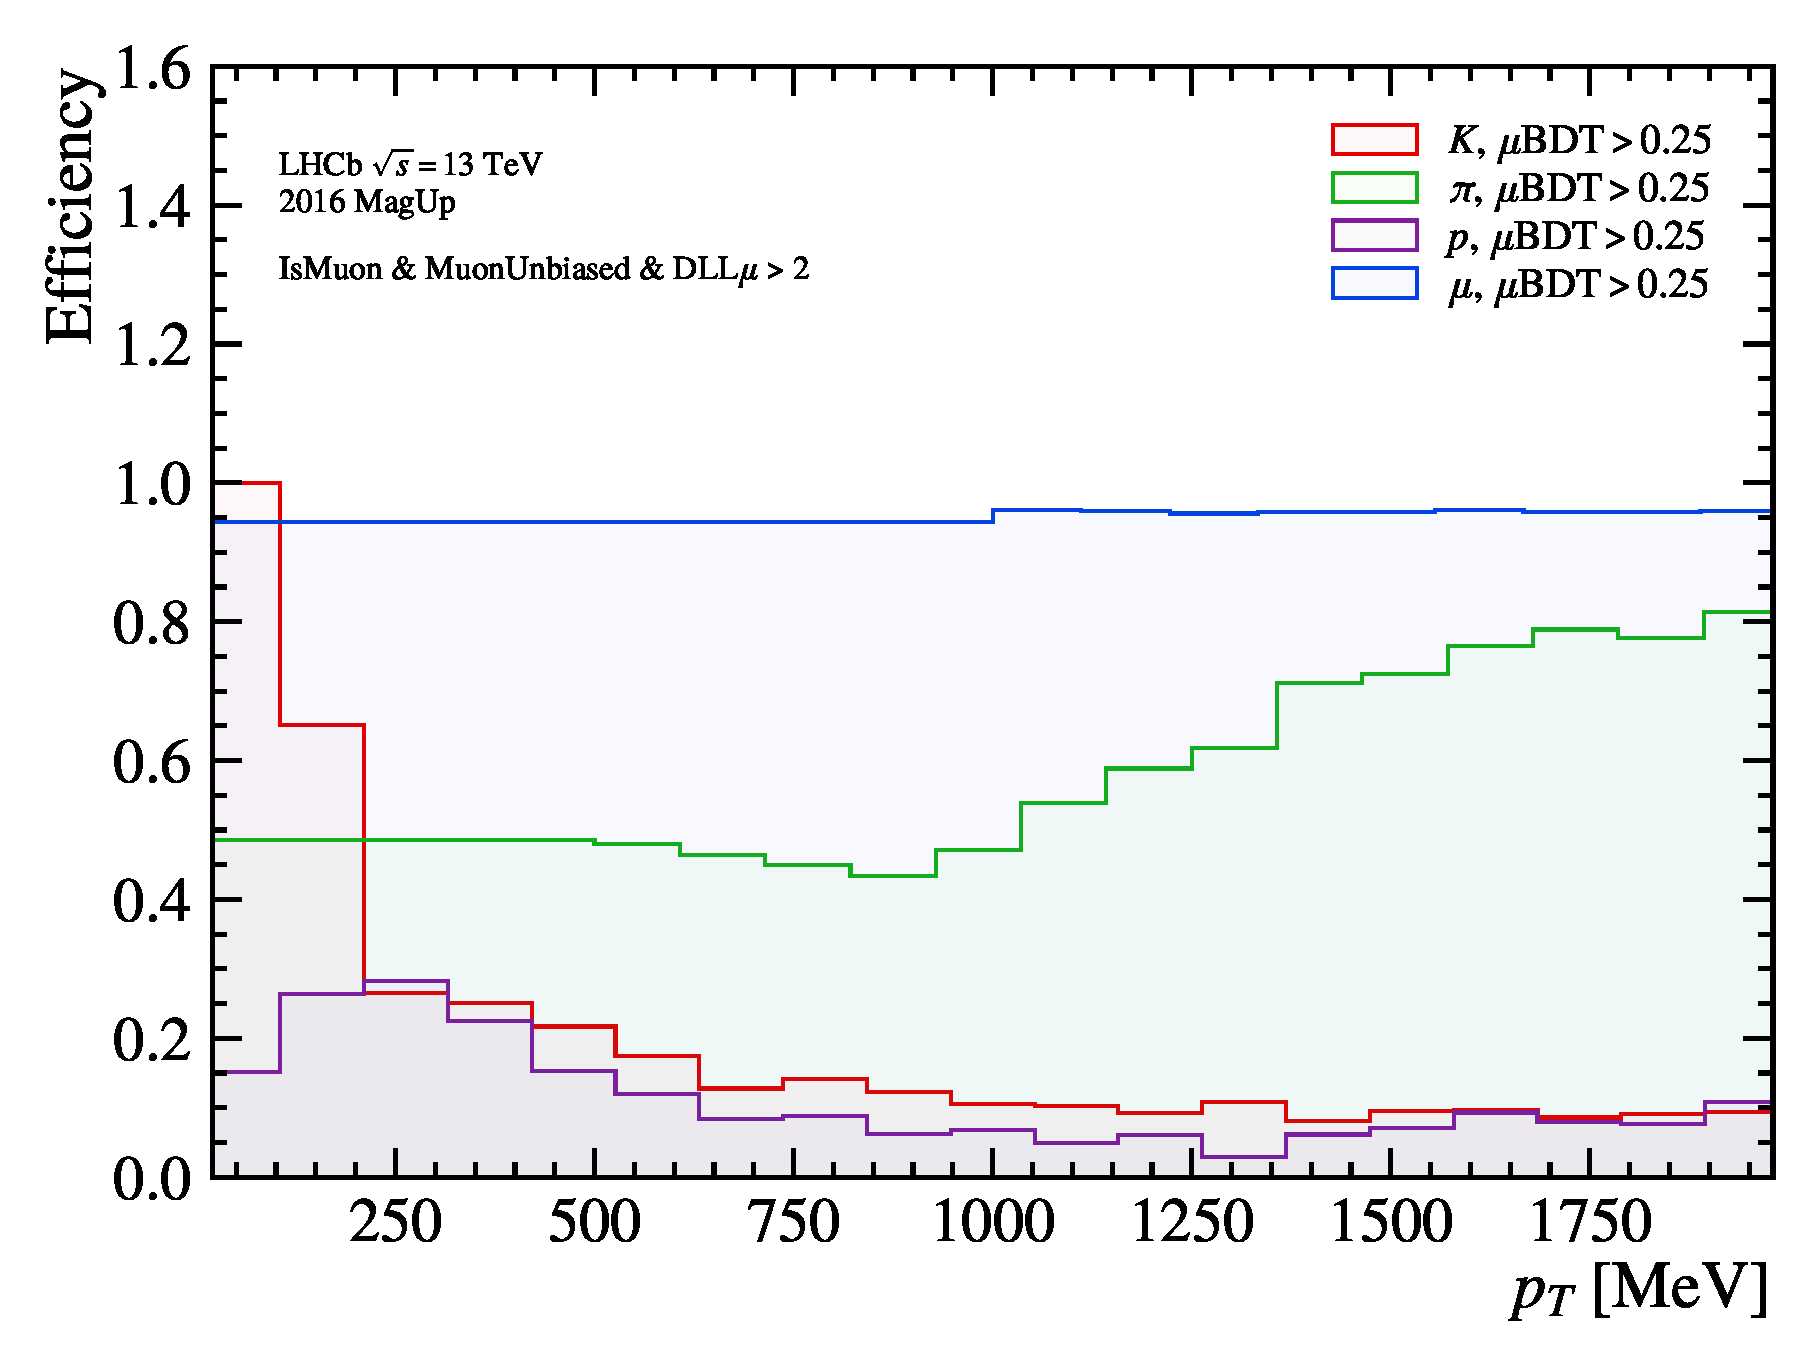
\includegraphics[width=0.45\textwidth]{./figs-selection/eff_Brunel_PT_up_pidcalib_ubdt_eff.pdf}
    \hspace{1em}
    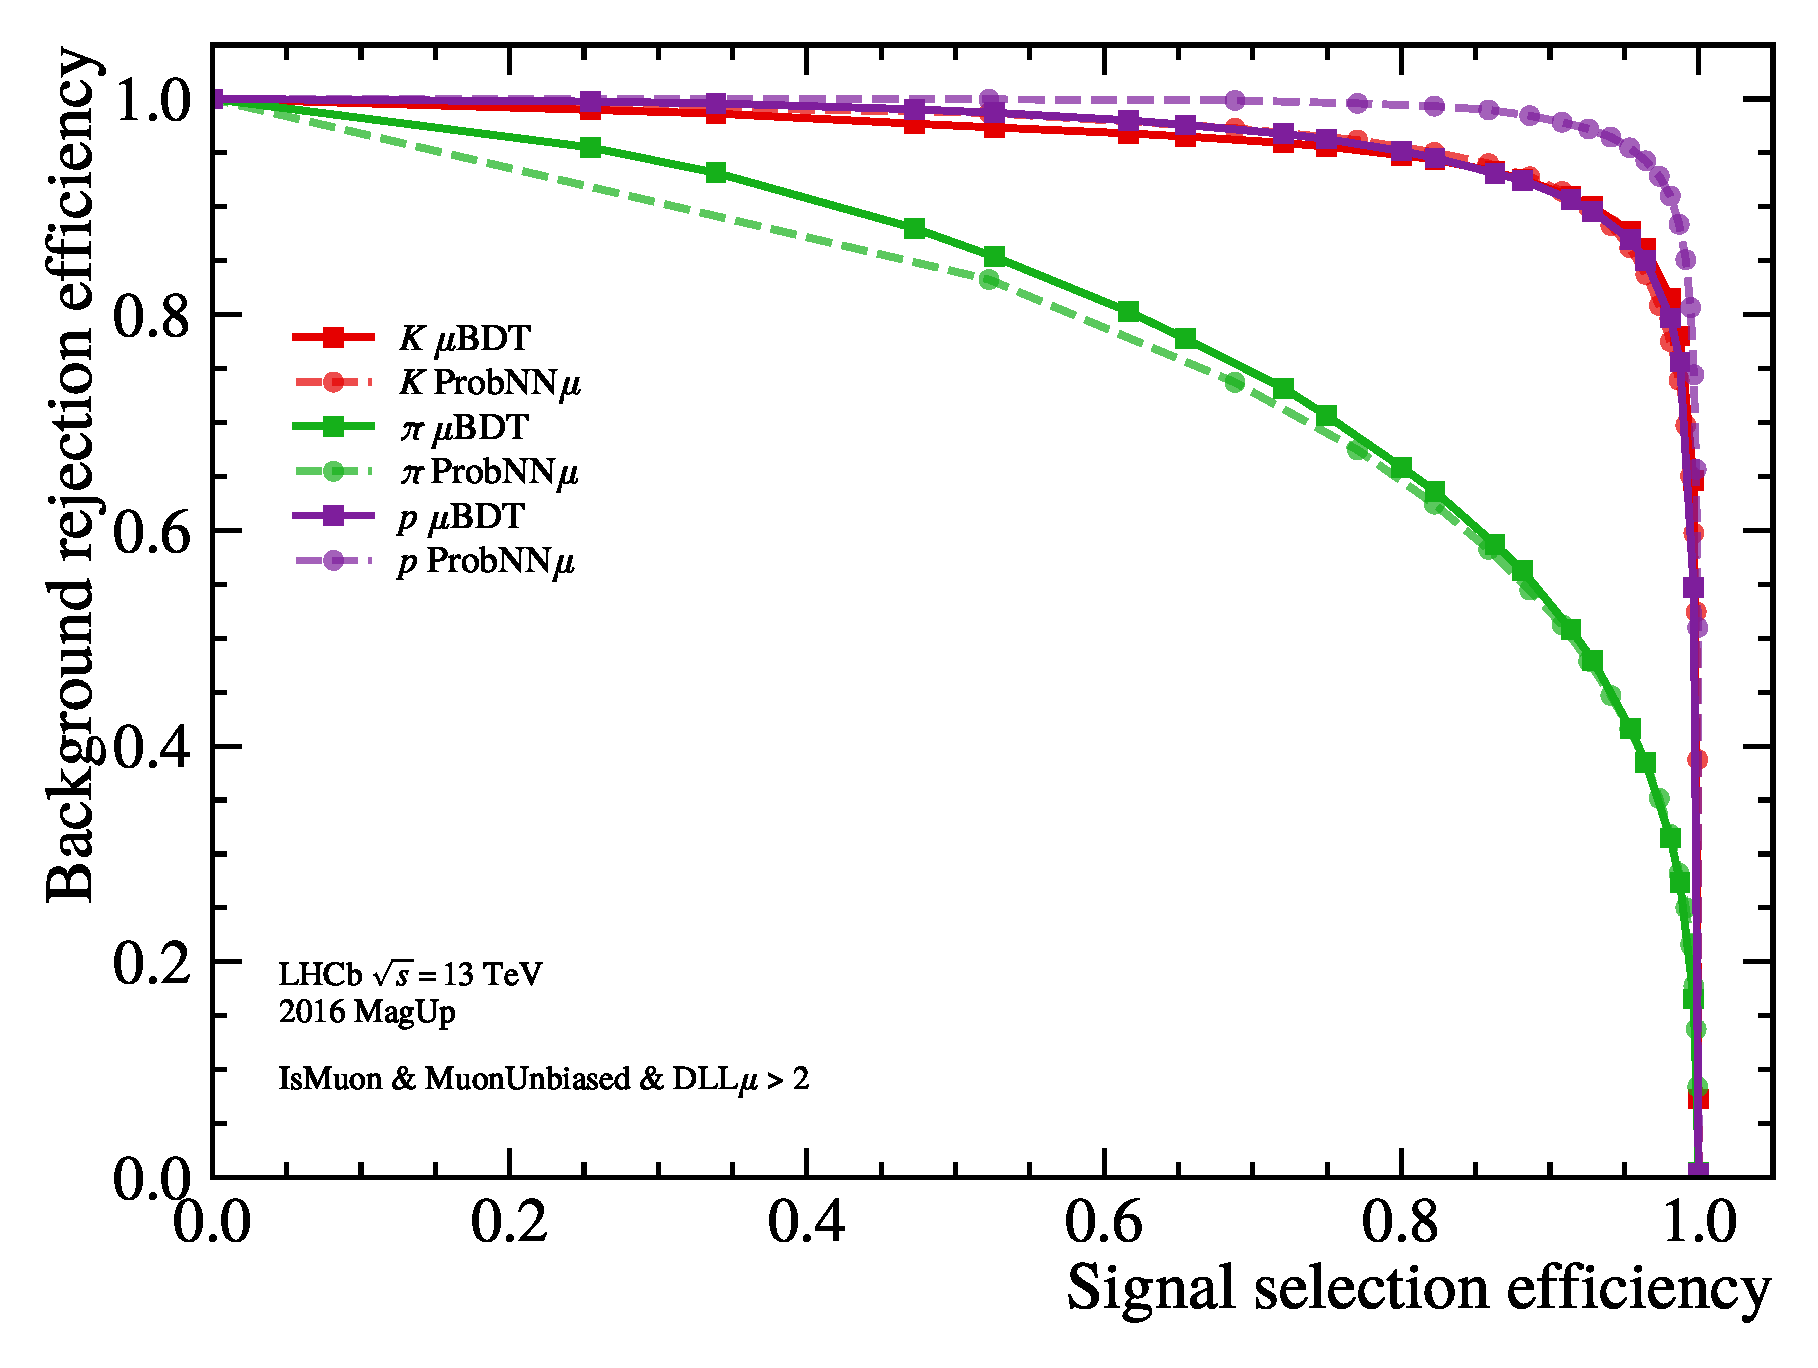
\includegraphics[width=0.45\textwidth]{./figs-selection/rej_v_eff_unbiased_Brunel_PT.pdf}

    \caption{
        Preliminary \UBDT study.
        Left: \UBDT \muon selection efficiency is flat in \pt, with
        global cut \isMuon \& $\text{\PID{\muon}}\! > 2$,
        and $\UBDT > 0.25$.
        Right: with the same global cut, \UBDT is more effective in rejecting
        \pion than LHCb official \ProbNN{\muon}.
        The \kaon rejection efficiencies are similar between the two;
        the $p$ rejection efficiency is lower for \UBDT, but the absolute
        rejection efficiency is high enough.
    }
    \label{fig:ubdt-eff}
\end{figure}



% CHANGES:
% chapter 2: divide into sub-sections (maybe)
%   introduce D**, DDX, background, comb. misID
%     one for D**, one for D** heavy
%   followed by introduction of skims
%  iso: signal sample; ctrl: control samples
%
% chapter 5:
%   5.2, define ghost and cocktail
%   all tracks -> long tracks, find the PT requirement
%   remove the 'likely due to ' part in 5.5.2
%   'refit a vertex' -> ?
%   5.5.2 'improved': forget about saving and ntuple stuff.
%
% chapter 6:
%   TOS and TIS in main text.
%
% chapter 9:
%   explain DiF more


% This table is based on the output of:
%   ./size_mc_samples.py -m detail -i 12573012 11574021 12773410
\begin{landscape}
\begin{table}[p]
    \caption{
        List of MC sample used in this analysis.
        Numbers are event on disk, not total simulated numbers.
    }
    \label{tab:mc-d0-dst}
    \centering\scriptsize
    \begin{longtable}{c|c|c|c|c|r|r|r|r}
        \toprule
        {\bf Group} &
        {\bf MC ID} &
        {\bf Decay mode} &
        {\bf Channels}  &
        {\bf Cocktail}  &
        {\bf\centering \makecell{2016 Sim09j \\ FullSim}} &
        {\bf\centering \makecell{2016 Sim09k \\ tracker-only}} &
        {\bf\centering \makecell{2017 Sim09k \\ tracker-only}} &
        {\bf\centering \makecell{2018 Sim09k \\ tracker-only}} \\
        \midrule
        \endhead
        norm.        & 12573012
                     & $\Bm \rightarrow \Dz \mun \neumb$
                     & \Dz & no
                     %%%%
                     & 3,564,053
                     & 45,564,529
                     & 47,965,869
                     & 64,386,408
                     \\
                     %%%%
                     & 11574021
                     & $\Bzb \rightarrow \Dstarp \mun \neumb$
                     & both & no
                     %%%%
                     & 3,012,029
                     & 85,470,057
                     & 81,075,745
                     & 103,168,826
                     \\
                     %%%%
                     & 12773410
                     & $\Bm \rightarrow \Dstarz \mun \neumb$
                     & \Dz & no
                     %%%%
                     & 4,003,029
                     & 129,200,391
                     & 134,602,735
                     & 169,664,396
                     \\
                     %%%%
        \midrule
        sig.         & 12573001
                     & $\Bm \rightarrow \Dz \taum \neutb$
                     & \Dz & no
                     %%%%
                     & 233,966
                     & 4,152,856
                     & 3,405,213
                     & 4,317,050
                     \\
                     %%%%
                     & 11574011
                     & $\Bzb \rightarrow \Dstarp \taum \neutb$
                     & both & no
                     %%%%
                     & 593,350
                     & 17,217,664
                     & 18,008,069
                     & 25,341,935
                     \\
                     %%%%
                     & 12773400
                     & $\Bm \rightarrow \Dstarz \mun \neumb$
                     & \Dz & no
                     %%%%
                     & 528,616
                     & 9,813,636
                     & 10,289,156
                     & 15,091,483
                     \\
                     %%%%
        \midrule
        $D^{**}$     & 11874430
                     & $\Bzb \rightarrow \D^{**+} \mun \neumb$
                     & both & $D_1^+,D_1^{'+}, D_2^{*+}, D_0^{*+}$
                     %%%%
                     & 2,865,898
                     & 46,653,556
                     & 45,469,066
                     & 58,082,278
                     \\
                     %%%%
                     & 11874440
                     & $\Bzb \rightarrow \D^{**+} \taum \neutb$
                     & both & $D_1^+,D_1^{'+}, D_2^{*+}, D_0^{*+}$
                     %%%%
                     & 35,322
                     & 375,581
                     & 519,245
                     & 561,800
                     \\
                     %%%%
                     & 12873450
                     & $\Bm \rightarrow \D^{**0} \mun \neumb$
                     & both & $D_1^0,D_1^{'0}, D_2^{*0}, D_0^{*0}$
                     %%%%
                     & 2,333,268
                     & 37,417,148
                     & 117,729,837
                     & 48,051,754
                     \\
                     %%%%
                     & 12873460
                     & $\Bm \rightarrow \D^{**0} \taum \neutb$
                     & both & $D_1^0,D_1^{'0}, D_2^{*0}, D_0^{*0}$
                     %%%%
                     & 112,138
                     & 618,529
                     & 598,526
                     & 744,330
                     \\
                     %%%%
        \midrule
        $D^{**}_H$   & 12675011
                     & $\Bm \rightarrow \D^{**0}_H (\rightarrow \Dz\pi\pi) \mun \neumb$
                     & \Dz & \cite{LHCb-ANA-2020-056}
                     %%%%
                     & 419,829
                     & 6,204,217
                     & 7,215,251
                     & 8,573,968
                     \\
                     %%%%
                     & 11674401
                     & $\Bzb \rightarrow \D^{**+}_H (\rightarrow \Dz\pi\pi) \mun \neumb$
                     & \Dz & \cite{LHCb-ANA-2020-056}
                     %%%%
                     & 353,015
                     & 6,997,221
                     & 6,746,518
                     & 12,956,078
                     \\
                     %%%%
                     & 12675402
                     & $\Bm \rightarrow \D^{**0}_H (\rightarrow \Dstarp\pi\pi) \mun \neumb$
                     & both & \cite{LHCb-ANA-2020-056}
                     %%%%
                     & 294,872
                     & 5,560,586
                     & 4,739,776
                     & 6,162,695
                     \\
                     %%%%
                     & 11676012
                     & $\Bzb \rightarrow \D^{**+}_H (\rightarrow \Dstarp\pi\pi) \mun \neumb$
                     & both & \cite{LHCb-ANA-2020-056}
                     %%%%
                     & 290,791
                     & 4,824,507
                     & 4,834,264
                     & 8,353,204
                     \\
                     %%%%
                     & 12875440
                     & $\Bm \rightarrow \D^{**0}_H (\rightarrow \Dstarz\pi\pi) \mun \neumb$
                     & \Dz & \cite{LHCb-ANA-2020-056}
                     %%%%
                     & 450,907
                     & 7,840,307
                     & 7,983,973
                     & 10,039,996
                     \\
                     %%%%
        \midrule
        $D^{**}_s$   & 13874020
                     & $\Bsb \rightarrow \D^{**+}_s (\rightarrow \Dz\Kp) \mun \neumb$
                     & \Dz & no
                     %%%%
                     & 259,166
                     & 1,654,215
                     & 1,732,571
                     & 2,214,625
                     \\
                     %%%%
                     & 13674000
                     & $\Bsb \rightarrow \D^{**+} \mun \neumb$
                     & \Dstar & $D_{s1}^{'+}, D_{s2}^{*+}$
                     %%%%
                     & 142,549
                     & 1,498,067
                     & 1,531,966
                     & 2,070,074
                     \\
                     %%%%
        \midrule
        $DDX$        & 11894600
                     & $\Bzb \rightarrow \Dz X_c (\rightarrow X' \mump \neumb) X$
                     & \Dz & \cite{LHCb-ANA-2020-056}
                     %%%%
                     & 1,062,375
                     & 36,888,835
                     & 37,826,396
                     & 49,768,186
                     \\
                     %%%%
                     & 12893600
                     & $\Bm \rightarrow \Dz X_c (\rightarrow X' \mump \neumb) X$
                     & \Dz & \cite{LHCb-ANA-2020-056}
                     %%%%
                     & 1,196,059
                     & 21,854,863
                     & 22,577,692
                     & 28,900,392
                     \\
                     %%%%
                     & 11894200
                     & $\Bzb \rightarrow \Dz D_s^- (\rightarrow X' \taum \neutb) X$
                     & \Dz & \cite{LHCb-ANA-2020-056}
                     %%%%
                     & 84,533
                     & 1,231,353
                     & 1,145,771
                     & 1,367,357
                     \\
                     %%%%
                     & 12893610
                     & $\Bm \rightarrow \Dz D_s^- (\rightarrow X' \taum \neutb) X$
                     & \Dz & \cite{LHCb-ANA-2020-056}
                     %%%%
                     & 255,725
                     & 2,818,348
                     & 2,625,208
                     & 4,834,213
                     \\
                     %%%%
                     %%%%
                     & 11894610
                     & $\Bzb \rightarrow \Dstarpm X_c (\rightarrow X' \mump \neumb) X$
                     & \Dstar & \cite{LHCb-ANA-2020-056}
                     %%%%
                     & 1,188,596
                     & 16,188,308
                     & 13,480,119
                     & 16,837,410
                     \\
                     %%%%
                     & 12895400
                     & $\Bm \rightarrow \Dstarpm X_c (\rightarrow X' \mump \neumb) X$
                     & \Dstar & \cite{LHCb-ANA-2020-056}
                     %%%%
                     & 365,215
                     & 7,000,178
                     & 7,459,109
                     & 6,798,676
                     \\
                     %%%%
                     & 11894210
                     & $\Bzb \rightarrow \Dstarp D_s^- (\rightarrow X' \taum \neutb) X$
                     & \Dstar & \cite{LHCb-ANA-2020-056}
                     %%%%
                     & 113,422
                     & 1,678,170
                     & 1,283,823
                     & 1,631,217
                     \\
                     %%%%
                     & 12895000
                     & $\Bm \rightarrow \Dstarp D_s^- (\rightarrow X' \taum \neutb) X$
                     & \Dstar & \cite{LHCb-ANA-2020-056}
                     %%%%
                     & 117,696
                     & 899,320
                     & 1,555,844
                     & 1,282,503
                     \\
                     %%%%
        \bottomrule
    \end{longtable}
\end{table}
\end{landscape}

\chapter{Emulation of detector responses on MC simulation}
\label{ref:mc-emulation}

To ensure the statistical uncertainties from MC samples are small compared to
that of data, it is typical to request MC samples with a size 4 times as large
as data.
Due to the sheer size of LHCb run 2 data (a factor of $\sim\!1.4$ for 2016
alone compared to full run 1), it is not computationally possible to generate
enough full simulation (FullSim) MC, where every detector response is simulated.

It is estimated in \cite{LHCb-INT-2019-025}
that about 85\% of the computation time is spent on simulating RICH and the
calorimeter system.
Tracker-only (TO) MC sets all but the tracking system of the detector to
passive material, making the simulation about 8 times faster than FullSim.
Hence, to reach target statistical uncertainties,
TO MC is (almost) exclusively used for this analysis.
Therefore, detector responses like trigger and particle identification (PID)
need to be emulated offline.
The emulation procedures for these responses are described in the rest of the
chapter.


\section{Trigger emulation}
\subsection{Emulation of L0Hadron TOS}

Recall that the L0 trigger requirements for this analysis are: Either \Dz
triggers L0 hadron (\Dz L0Hadron TOS\footnote{
    TOS: Triggered On Signal. Can be used as a noun or a verb.
    For more information about trigger TIS, TOS, TISTOS, and TOB, refer to
    \cref{appx:trigger-cat}.
}) or
the rest of the event aside from \B (and its decay chain) triggers at least
one L0 trigger
(\B L0Global TIS\footnote{
    TIS: Triggered Independent of Signal.
    In this case \B is the signal track, and the rest of event is inspected to
    determine if it triggers at least a L0 trigger.
}).

The L0 hadron is triggered when the sum of the transverse energy\footnote{
    Defined as: $E_T \equiv \sqrt{m^2 + p^2} \sin\theta$.
    In massless limit, $E_T = p_T$.
} $E_T$ deposited
in a single $2 \times 2$ HCAL cluster is above a set threshold\footnote{
    See Table 1 in \cite{LHCb-DP-2019-001} for year-by-year thresholds of each
    L0 trigger.
}, as described in \cite{LHCb-DP-2019-001}.
For L0Hadron TOS, it is required that for all HCAL clusters associated with the
signal track (\Dz in this case), with association predicted by the tracking
system,
the highest $E_T$ is above the triggering threshold.

Tracker-only MC records the tracker-predicted position where a track hits the
calorimeters.
Hence, though the triggering variable $E_T$ is not accessible,
variables related to $E_T$, or, equivalently, trigger decision, are.
It is conceivable that L0Hadron TOS can be emulated by providing
the relevant variables and the trigger decision to train some regressor,
which can in turn be used to predict trigger decisions based on the training
variables alone, without requiring emulating $E_T$ at all.
Below the emulation procedure, inspired by \cite{LHCb-INT-2019-025}, is
described:

\begin{enumerate}
    \item The \smalltt{TupleToolL0Calo} tool is configured to save HCAL
        information.
    \item The training variables, listed in \cref{tab:l0-hadron-emu-vars}, and
        the trigger decision from a FullSim MC of decay
        $\Bz \rightarrow \Dstarp \mu \nu$, a normalization mode,
        is used to train \xgboost, a BDT-based regressor.
    \item Once the model is trained, with just the training variables,
        \xgboost predicts the probabilities of events passing L0 hadron trigger.
    \item The probabilities are applied as weights to a separate validation
        sample of the same FullSim MC to check the quality of the emulation.
        It is shown in \cref{fig:l0hadron-tos-emu} that emulated L0Hadron TOS
        trigger has excellent agreement with \emph{simulated} trigger in
        FullSim.
\end{enumerate}

\begin{table}[htb]
    \caption{Variables used to train \xgboost for L0 hadron emulation.}
    \label{tab:l0-hadron-emu-vars}
    \centering
    \begin{tabular}{cc}
        \toprule
        Group       & Variables \\
        \midrule
        Event-level & nTracks \\
        \Dz         & $p$, $p_T$ \\
        \midrule
        \Km         & \makecell{
                      $p$, $p_T$,
                      real $E_T$\parnote{
                          This is the $E_T$ measured by the tracker.
                          In massless limit, $E_T = p_T$.
                      }, \\
                      HCAL $x$-projection, HCAL $y$-projection,
                      HCAL region\parnote{
                          This indicates whether the hits are in the inner or
                          outer region of HCAL.
                          The outer region has a coarser granularity than the
                          inner, thus it is more likely that the energies from
                          \Km and \pip are deposited in the same cluster,
                          enhancing L0Hadron TOS efficiency.
                      }} \\
        \midrule
        \pip        & same as \Km \\
        \bottomrule
    \end{tabular}
    \begin{flushleft}
        \parnotes
    \end{flushleft}
\end{table}

% Generated in //lhcb-ntuples-gen/studies/trigger_emulation-l0_hadron_tos_debug:
% By running:
%   git annex get .
%   debug_l0hadron.py
% in the folder specified above.
\begin{figure}
    \centering
    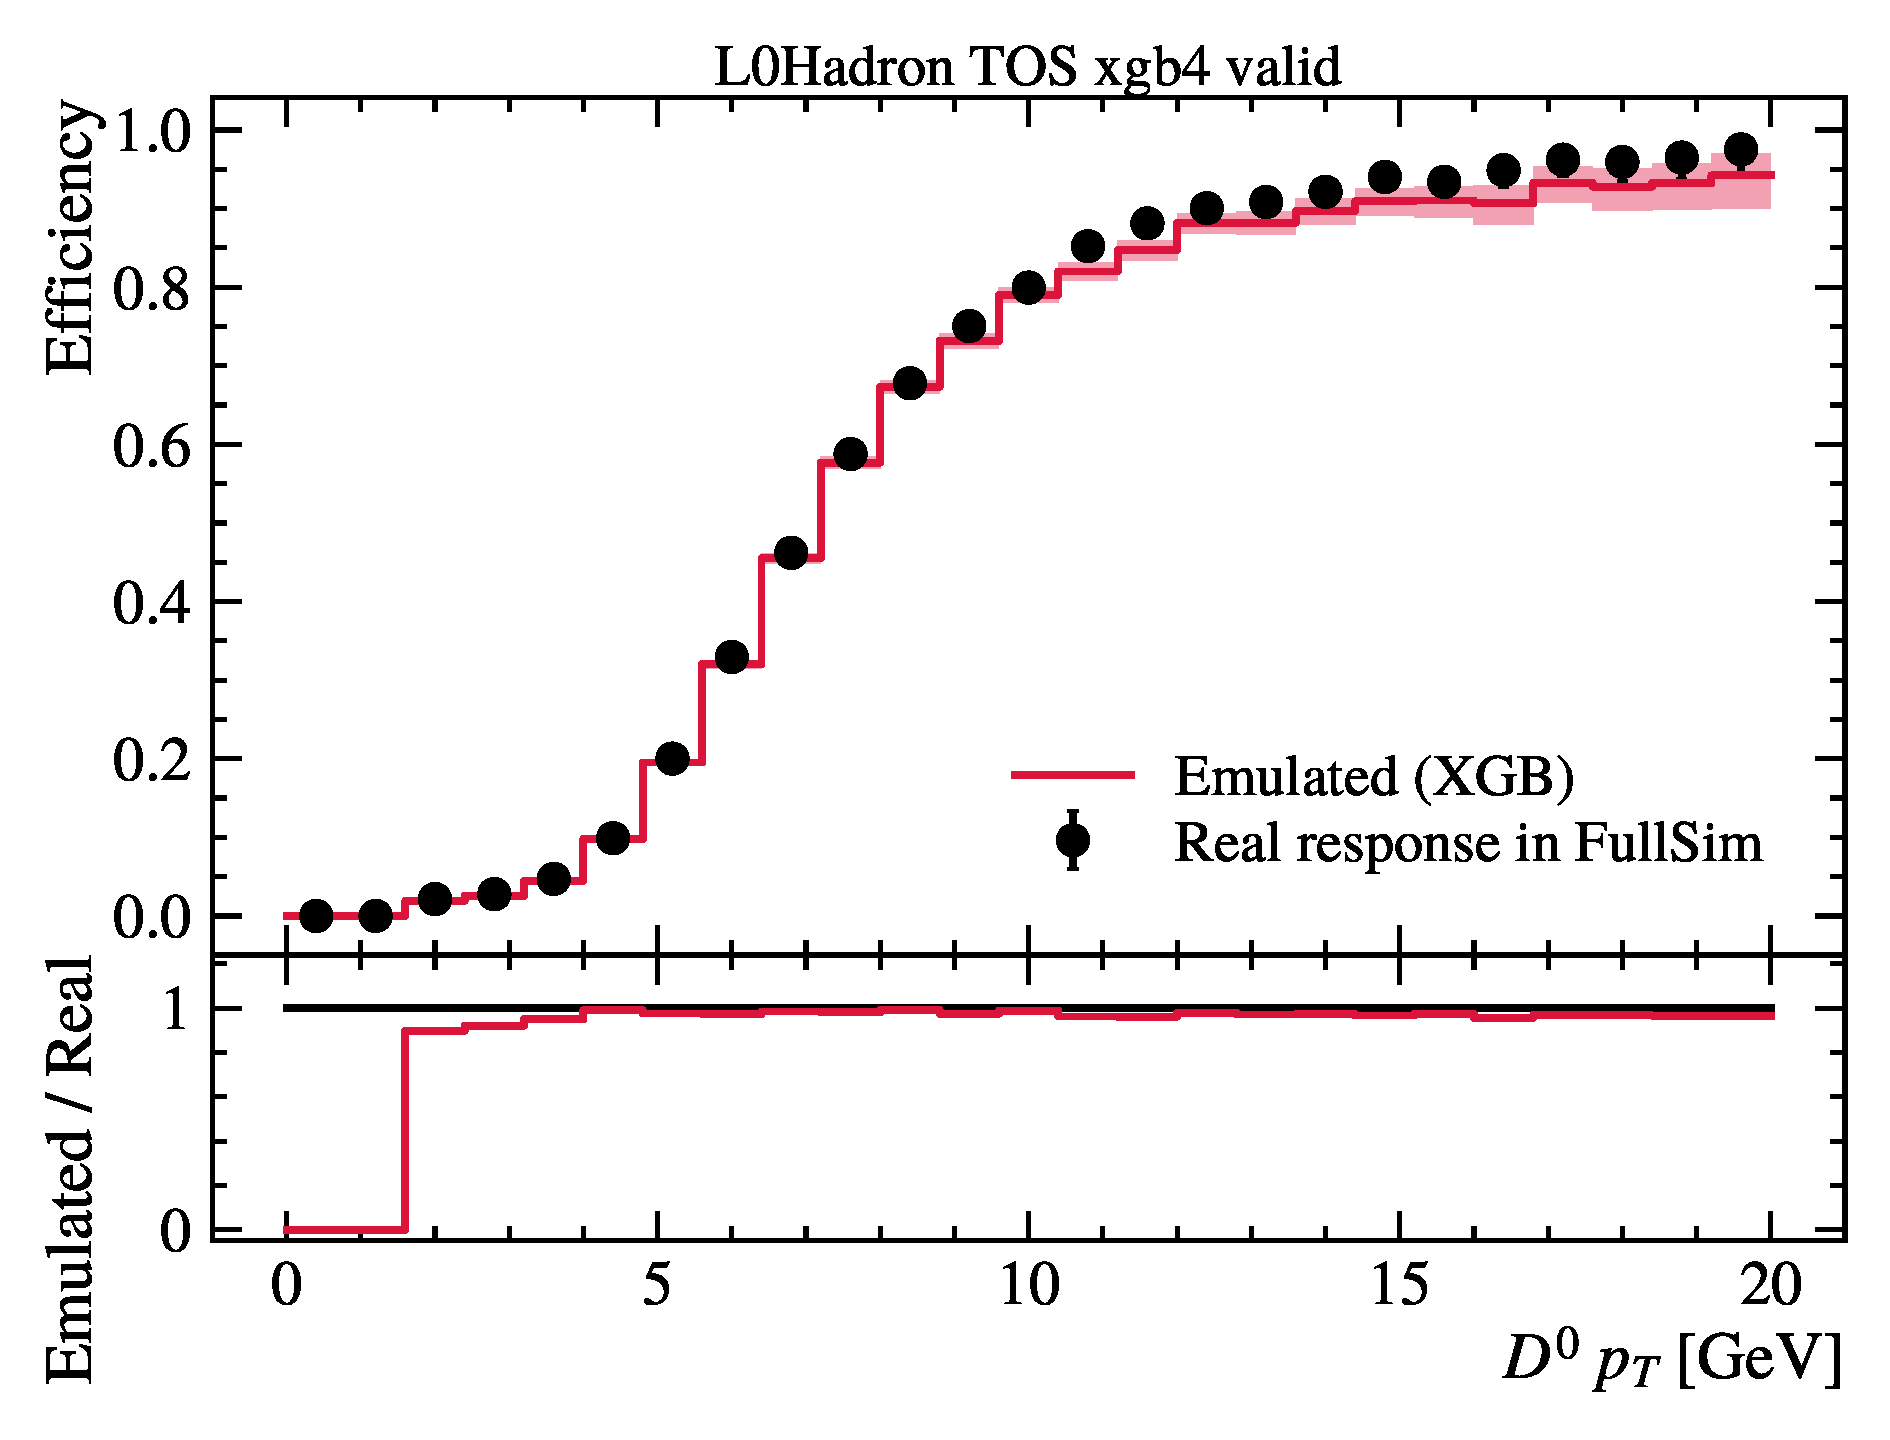
\includegraphics[width=0.7\textwidth]{./figs-mc-emulation/emulate-l0hadron-tos/b0_L0Hadron_TOS_xgb4_valid_d0_pt.pdf}
    \caption{
        The emulated trigger probabilities applied as a weight to FullSim has
        excellent agreement with real L0Hadron TOS trigger \emph{simulated} in
        FullSim.
    }
    \label{fig:l0hadron-tos-emu}
\end{figure}


\subsection{Emulation of L0Global TIS}

As discussed before, L0Global TIS is determined by \emph{the rest of event}
(everything but the reconstructed \B decay chain) which is \emph{not saved}
after event reconstruction.
Therefore, a completely different approach is needed for its emulation.

Instead of predicting event-by-event L0Global TIS probability based on the
properties of the rest of event, it is possible to measure L0Global TIS as
efficiencies binned in \emph{some reconstructed variables\footnote{
    The choice of variables will be discussed later.
}} externally,
then apply L0Global TIS efficiencies based on the bin the event falls in.

In addition, for hadron colliders,
the rest of event is \emph{busy} due to hadronization:
Indeed, for data reconstructed in
$\Bm \rightarrow \Dz (\rightarrow \Km \pip) \mun \neumb$ mode which is used in
this analysis,
the average number of tracks per event is 170,
whereas the selected \Dz\mun final state contains only 3 tracks (\Km, \pip, and
\mun, as \Dz and \Bm are reconstructed from these tracks)!
Therefore, it can be argued that the rest of event are essentially the same
between different reconstructions,
and L0Global TIS efficiencies are portable across different \B decay modes.

Assuming the L0Global TIS efficiencies can be measured in a data
sample reconstructed in a particular decay mode, the measured efficiencies
can be applied to TO MC as weights regardless of the decays.
This has the added benefit of L0Global TIS efficiencies agreeing with data by
definition, so it does not need additional data/MC correction.

To summarize, if the following assumptions hold, then the emulation outlined
above should work:

\begin{enumerate}
    \item The L0Global TIS efficiencies can be measured in data.
    \item The L0Global TIS efficiencies do not depend on \B decay mode.
\end{enumerate}

Before we proceed, let us define L0Global TIS efficiency
$\epsilon_\text{L0Global TIS}$ more precisely.
According to \cite{LHCb-PUB-2014-039}, in LHCb $\epsilon_\text{L0Global TIS}$
is conventionally defined as:

\begin{equation}
    \label{eqn:eff-l0global-tis}
    \epsilon_\text{L0Global TIS} \equiv
    \frac{N_\text{L0Global TIS \& selected}}{N_\text{selected}}
\end{equation}
which is not directly evaluable in real data, as $N_\text{selected}$ refers to
number of selected events \emph{regardless} of their trigger decisions, which is
not measurable (in data).

However, the conditional efficiency, $\epsilon_\text{L0Global TIS|L0Muon TOS}$,
is measurable:

\begin{equation}
    \epsilon_\text{L0Global TIS|L0Muon TOS} \equiv
    \frac{N_\text{L0Global TIS \& L0Muon TOS \& selected}}{
          N_\text{L0Muon TOS \& selected}}
\end{equation}
as long as L0Muon on signal and all L0 triggers (L0Global) on rest of event are
uncorrelated,
$\epsilon_\text{L0Global TIS|L0Muon TOS}$ is equivalent to
$\epsilon_\text{L0Global TIS}$.
Such a method is called \emph{TISTOS method}.
Unfortunately, there is a correlation between the two triggers due to
the fact that \bbbar are produced in pairs, making kinematics of the selected
signal \B meson and the background \Bbar meson, part of rest of event,
correlated.

Still, it is argued in \cite{LHCb-PUB-2014-039} that L0Global TIS and L0Muon TOS
are \emph{uncorrelated} in a small region of signal \B phase space.
Thus, it is possible to measure $\epsilon_\text{L0Global TIS}$ \emph{binned} in
\B kinematic variables with TISTOS method.

In \cite{LHCb-INT-2019-025} it is checked that binned
$\epsilon_\text{TISTOS} = \epsilon_\text{TIS}$ in
$\B \rightarrow \jpsi K$ FullSim MC\footnote{
    TISTOS does not always work. See \cref{appx:suppl:l0global-tis} for a
    counter example.
}, and evaluated
$\epsilon_\text{L0Global TIS}$ on data reconstructed in $\jpsi K$, binned
in $\log(p_z)$ and $\log(p_T)$ of the \B meson.
It is also checked that the efficiencies are portable among
$\B \rightarrow \jpsi K$, $\B \rightarrow \Dp \muon \neu$, and
$\B \rightarrow \Dp \tauon \neu$ decays with MC samples.
%%%%
In \cref{fig:l0global-tis-portable} it is checked
that the portability still holds for this analysis in
$\B \rightarrow \Dstarp \muon \neu$ and $\B \rightarrow \Dstarp \tauon \neu$.
The efficiencies obtained in \cite{LHCb-INT-2019-025} are applied to all TO MC
samples in this analysis, with binning variables changed to true momenta, as
the reconstruction in this analysis contains missing neutrino(s),
whereas $\jpsi K$ does not.

% Generated in /lhcb-ntuples-gen/studies/trigger_emulation-l0_global_tis_debug:
% By running:
%   debug_l0global.py
% in the folder specified above.
\begin{figure}[ht]
    \centering
    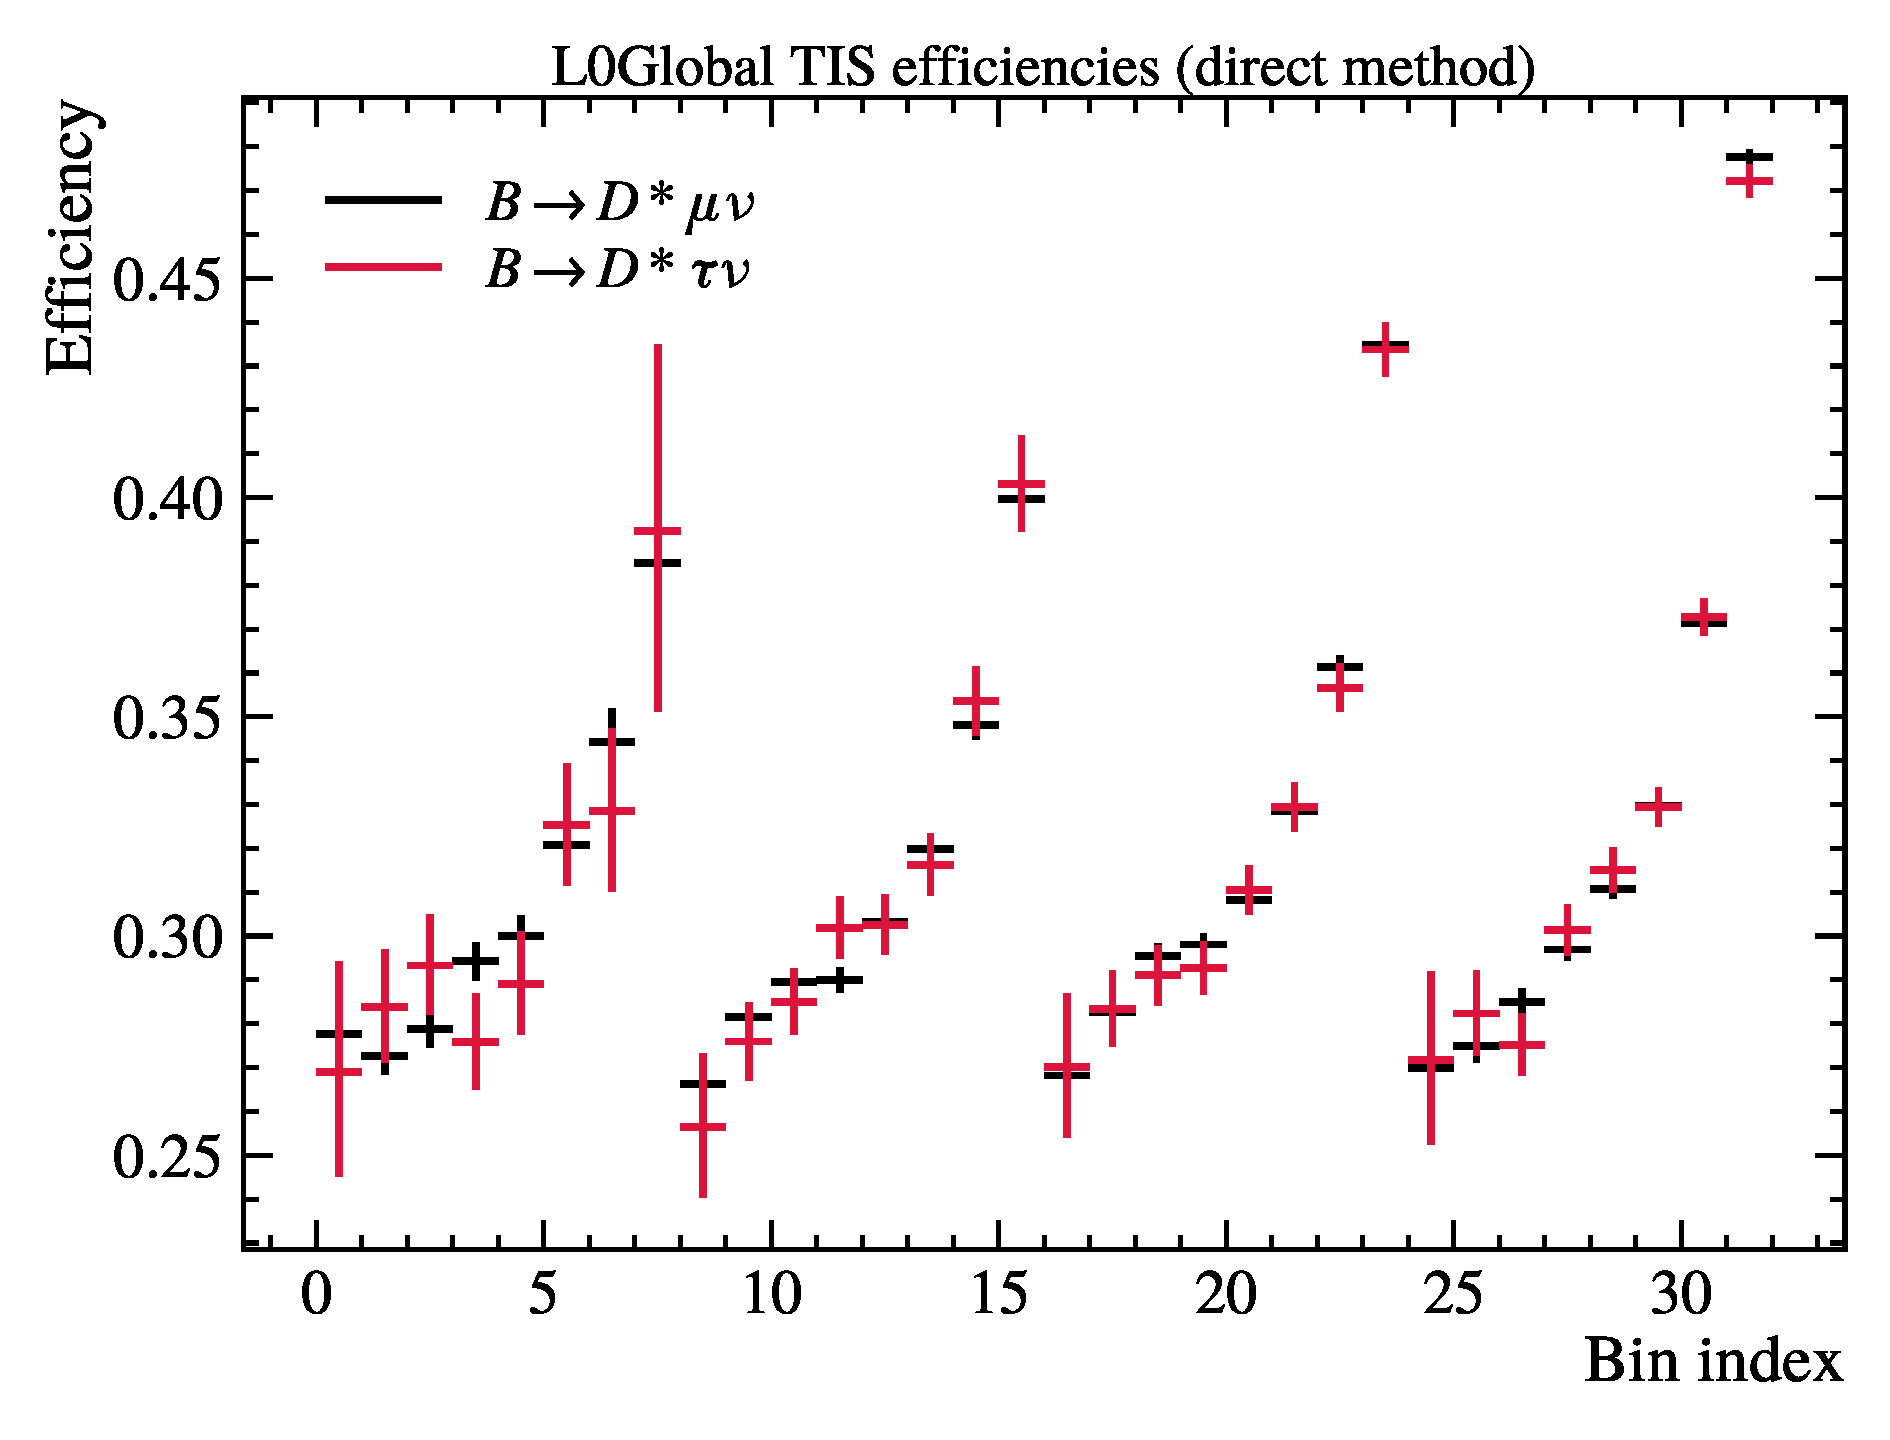
\includegraphics[width=0.32\textwidth]{
        ./figs-mc-emulation/emulate-l0global-tis/l0_global_tis_eff_bin_idx_dir.pdf
    }
    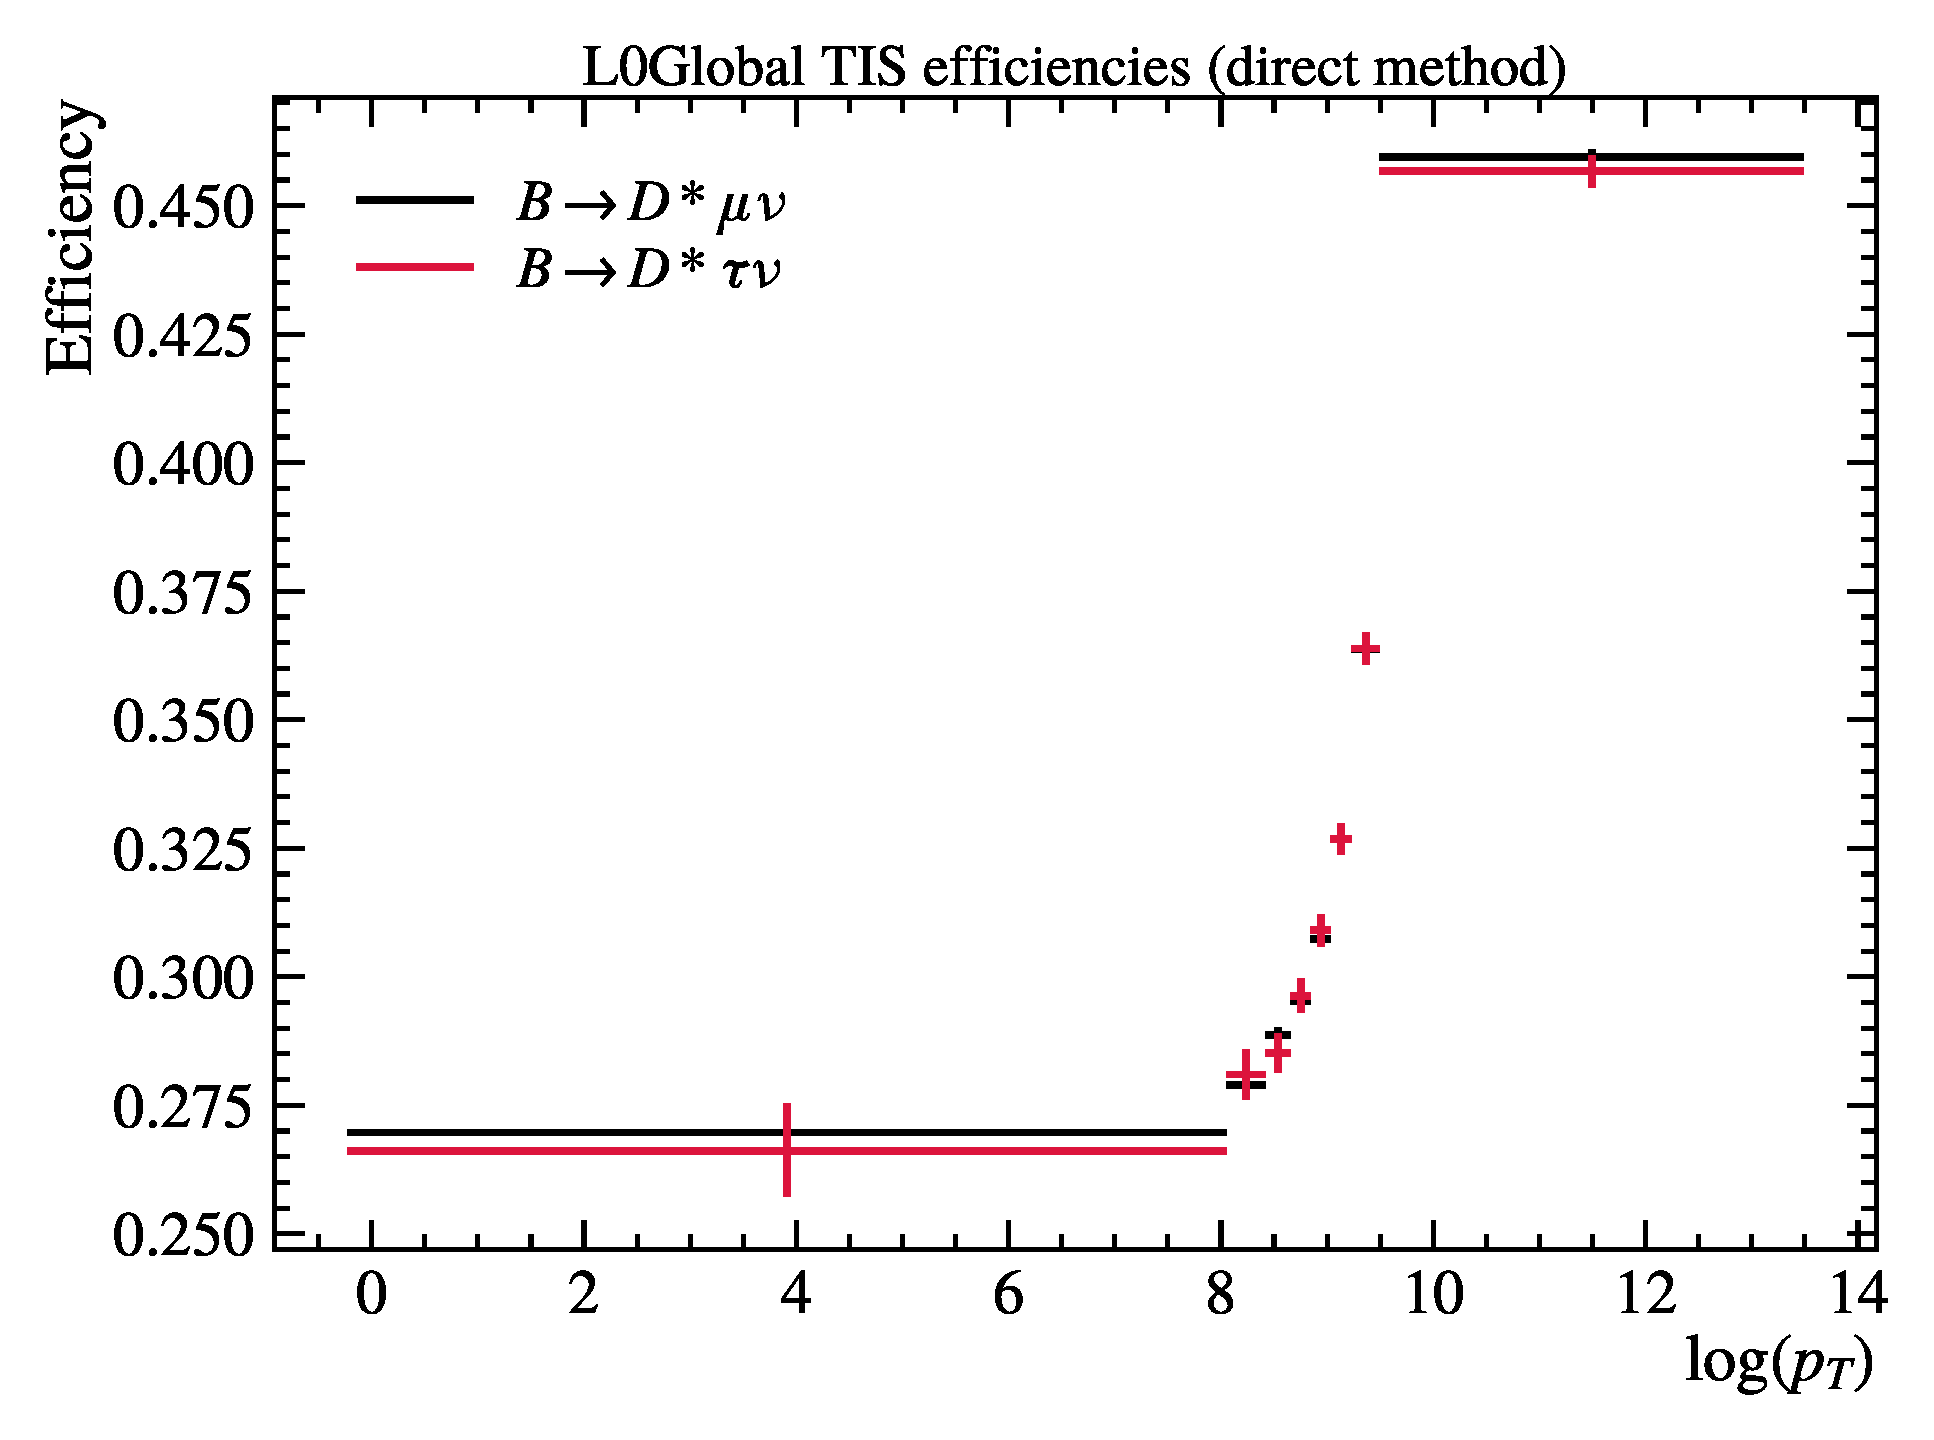
\includegraphics[width=0.32\textwidth]{
        ./figs-mc-emulation/emulate-l0global-tis/l0_global_tis_eff_log_pt_dir.pdf
    }
    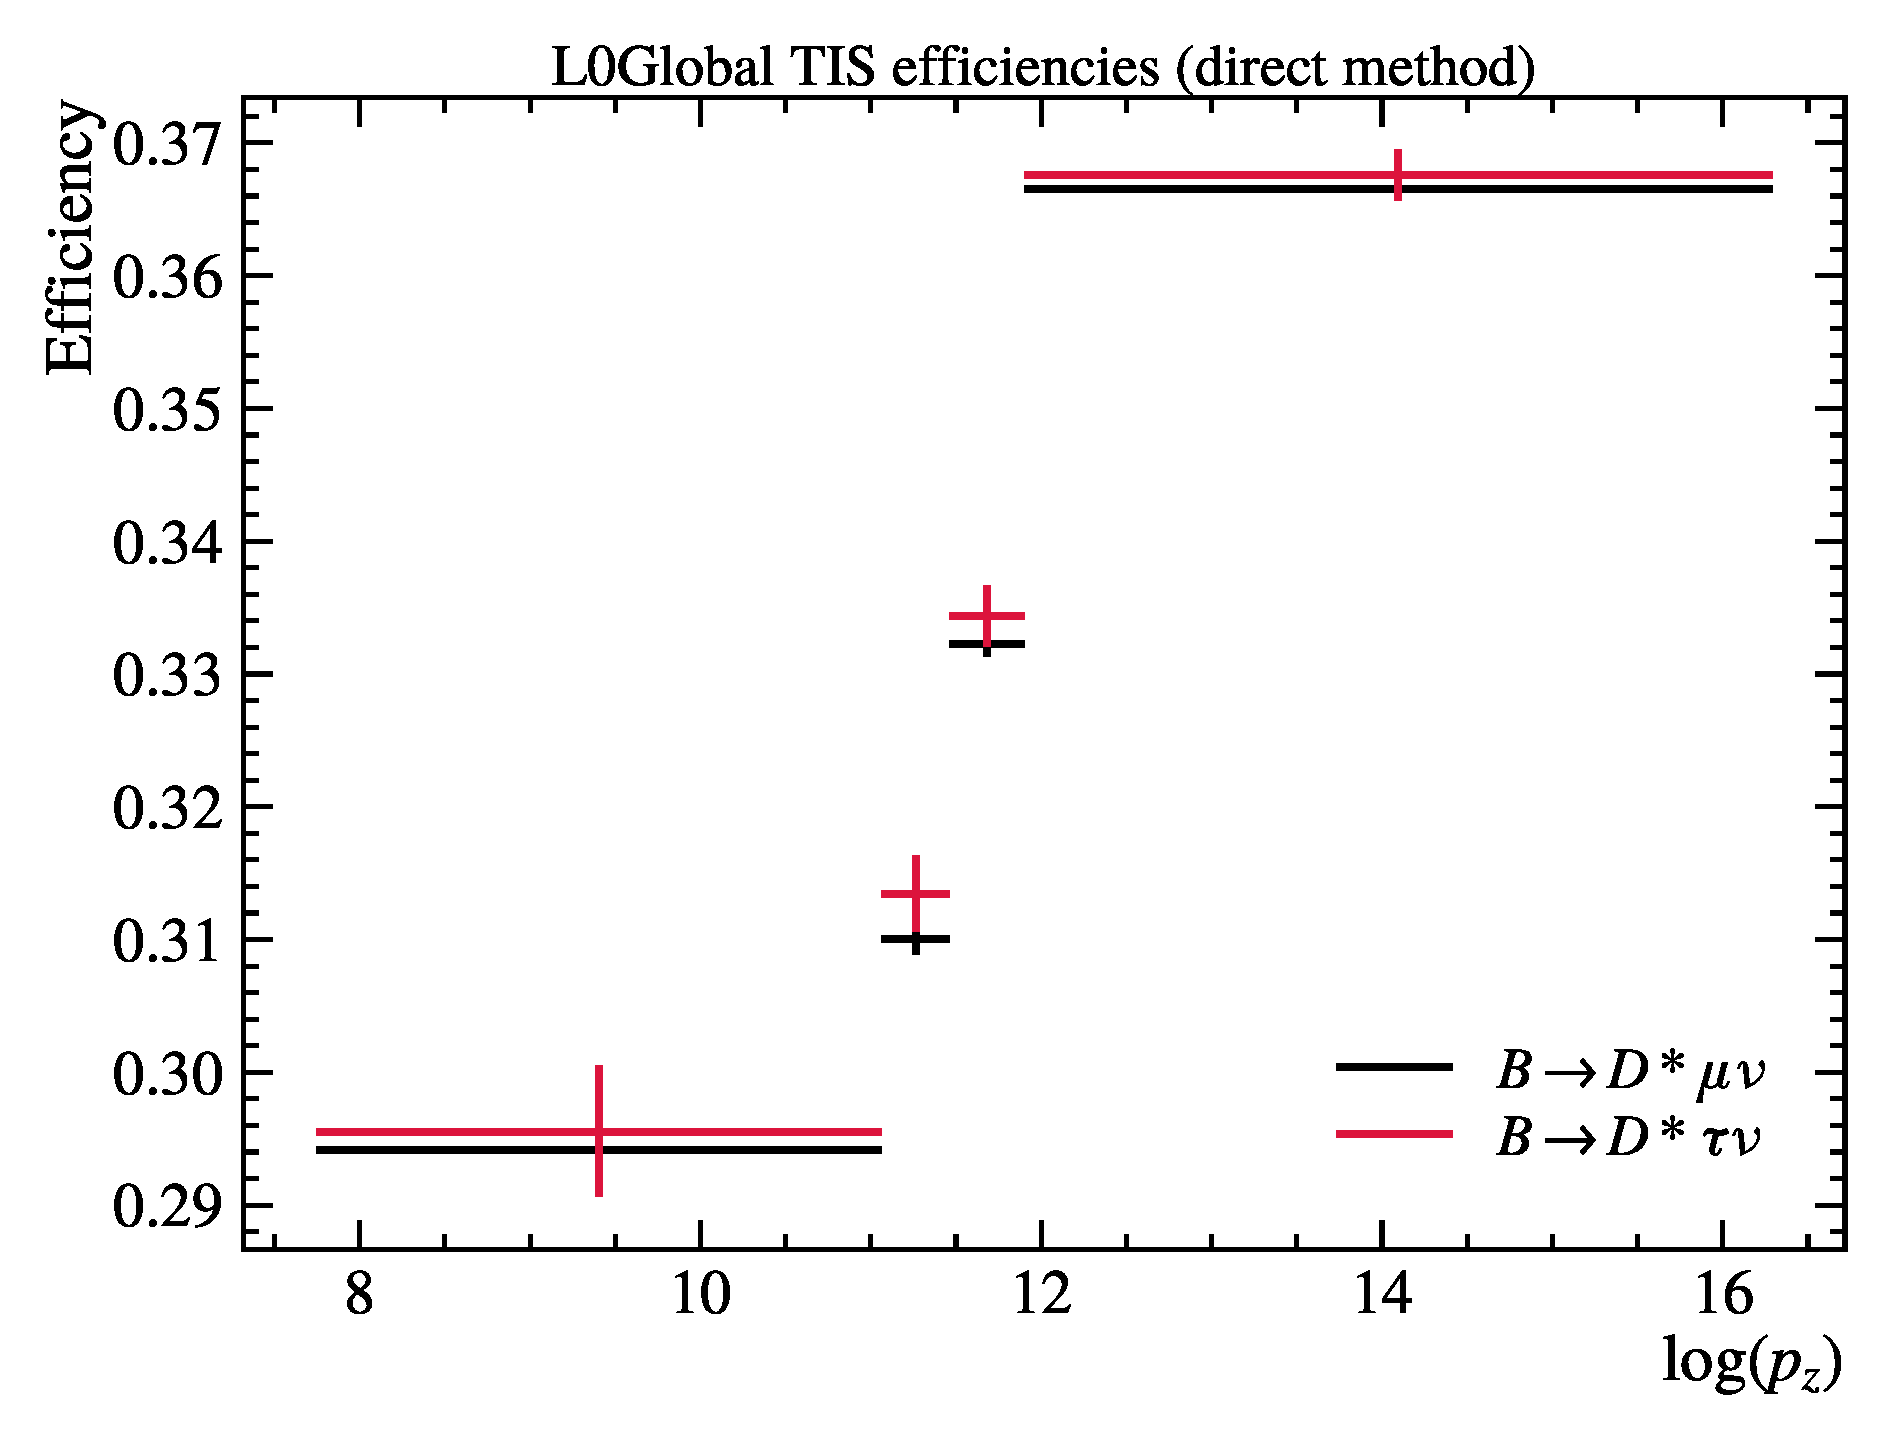
\includegraphics[width=0.32\textwidth]{
        ./figs-mc-emulation/emulate-l0global-tis/l0_global_tis_eff_log_pz_dir.pdf
    }
    \caption[Check that L0Global TIS is portable among signal and normalization MC modes]{
        Check that L0Global TIS is portable among signal and normalization MC modes

        The $p_T$ and $p_z$ momenta are MC true momenta of the $B$ meson.
        Bin index represents the index from an unrolled 2D
        true-$p_T$-true-$p_z$ histogram.
        Efficiencies are evaluated according to \cref{eqn:eff-l0global-tis},
        as the MC samples used here are \emph{not} filtered on trigger decision,
        so $N_\text{selected}$ can be evaluated directly.

        Efficiencies are in good agreement across all bins.
    }
    \label{fig:l0global-tis-portable}
\end{figure}


\subsection{Correlation between L0Hadron TOS and L0Global TIS}
\label{sec:emulation-for-to-mc:correlation-tos-tis}

L0 triggers have a global event cut on the number of SPD hits.
For all but the DiMuon trigger\footnote{
    Ignore Muon high \pt line for now.
}, the cut is placed at 450; for DiMuon, 900,
as listed in \cite{LHCb-INT-2019-025}.
For events that are both \emph{TIS and TOS}, a non-trivial correlation is
introduced by this cut, because it affects the L0 TIS efficiencies
inconsistently:
On a small patch of the signal \B phase space,
for events that are TIS on \emph{non-DiMuon}, TIS and TOS efficiency is:

\begin{equation}
    \epsilon_\text{TIS and TOS} =
        \epsilon_\text{L0-non-DiMuon TIS} \cdot \epsilon_\text{L0Hadron TOS}
\end{equation}

For L0DiMuon TIS only, however, its efficiency is affected by the SPD cut:
\begin{align}
    \epsilon_\text{L0DiMuon TIS \& nSPDhits < 450} & \neq
        \epsilon_\text{L0DiMuon TIS} \\
    \Rightarrow \epsilon_\text{TIS and TOS} & =
            \epsilon_\text{L0DiMuon TIS \& nSPDhits < 450} \cdot
            \epsilon_\text{L0Hadron TOS} \\
        & \neq
        \epsilon_\text{L0DiMuon TIS} \cdot \epsilon_\text{L0Hadron TOS}
\end{align}

Therefore:
\begin{align}
    \epsilon_\text{TIS and TOS} & =
        (\epsilon_\text{L0-non-DiMuon TIS} +
         \epsilon_\text{DiMuon TIS \& nSPDhits < 450}) \cdot
         \epsilon_\text{L0Hadron TOS} \\
    & \neq
        \underbrace{\epsilon_\text{L0Global TIS}}_{
            = \epsilon_\text{L0-non-DiMuon TIS} +
              \epsilon_\text{L0DiMuon TIS}
         } \cdot\; \epsilon_\text{L0Hadron TOS}
\end{align}

To minimize the correlation, a $\text{nSPDhits} < 450$ is applied on all data
samples\footnote{
    It is applied on the $\jpsi K$ sample as well, the one used to obtain
    binned L0Global TIS efficiencies.
    For TO MC, there is no nSPDhits variable.
}, which removes about an additional 4.4\% of candidates for both \Dz and
\Dstar channel.
After the SPD cut is applied, it is checked that
$\epsilon_\text{TIS or TOS} \approx \epsilon_\text{TIS} + \epsilon_\text{TOS} -
\epsilon_\text{TIS} \cdot \epsilon_\text{TOS}$
in \cite{LHCb-INT-2019-025},
that is, TIS efficiencies can be considered as uncorrelated from
TOS efficiencies.


\subsection{Emulation of Hlt1TrackMVA and Hlt1TwoTrackMVA}

The event selection requires that either $K$ or $\pi$ is TOS on Hlt1TrackMVA,
or \Dz is TOS on Hlt1TwoTrackMVA.
The single track Hlt1TrackMVA requires a track that has score based on
$p_T$ and \ipChiSq to be above some threshold;
the two track Hlt1TwoTrackMVA feeds the $p_T$ and \ipChiSq of both tracks to
a MatrixNet MVA, requiring the two-track combination to pass MVA selection.

All required variables are present in TO MC, and are extracted by adding
a tool\footnote{
    Named \lstinline{RelInfoHLT1Emulation}, available at
    \url{https://github.com/umd-lhcb/TrackerOnlyEmu/tree/master/davinci/Phys},
    courtesy of the authors of \cite{LHCb-INT-2019-025}.
} to event reconstruction.

The HLT1 triggers also require events to pass Global Event Cuts (GEC).
There is also an online-offline difference:
The real HLT1 triggers uses VELO-TT tracks, whereas the emulation can use
VELO tracks only, therefore, additional cuts and a 4.2\% penalty factor are
imposed to account for the differences.
The HLT1 trigger cuts and GEC are listed in \cite{LHCb-INT-2019-025}.
The emulated HLT1 are in good agreement with the real response in FullSim, as
can be seen in \cref{fig:hlt1-trackmva-emu,fig:hlt1-twotrackmva-emu}.

% Generated in /lhcb-ntuples-gen/studies/plot-trigger_emulation, run the script:
%   trigger_emulation.sh
\begin{figure}[ht]
    \centering
    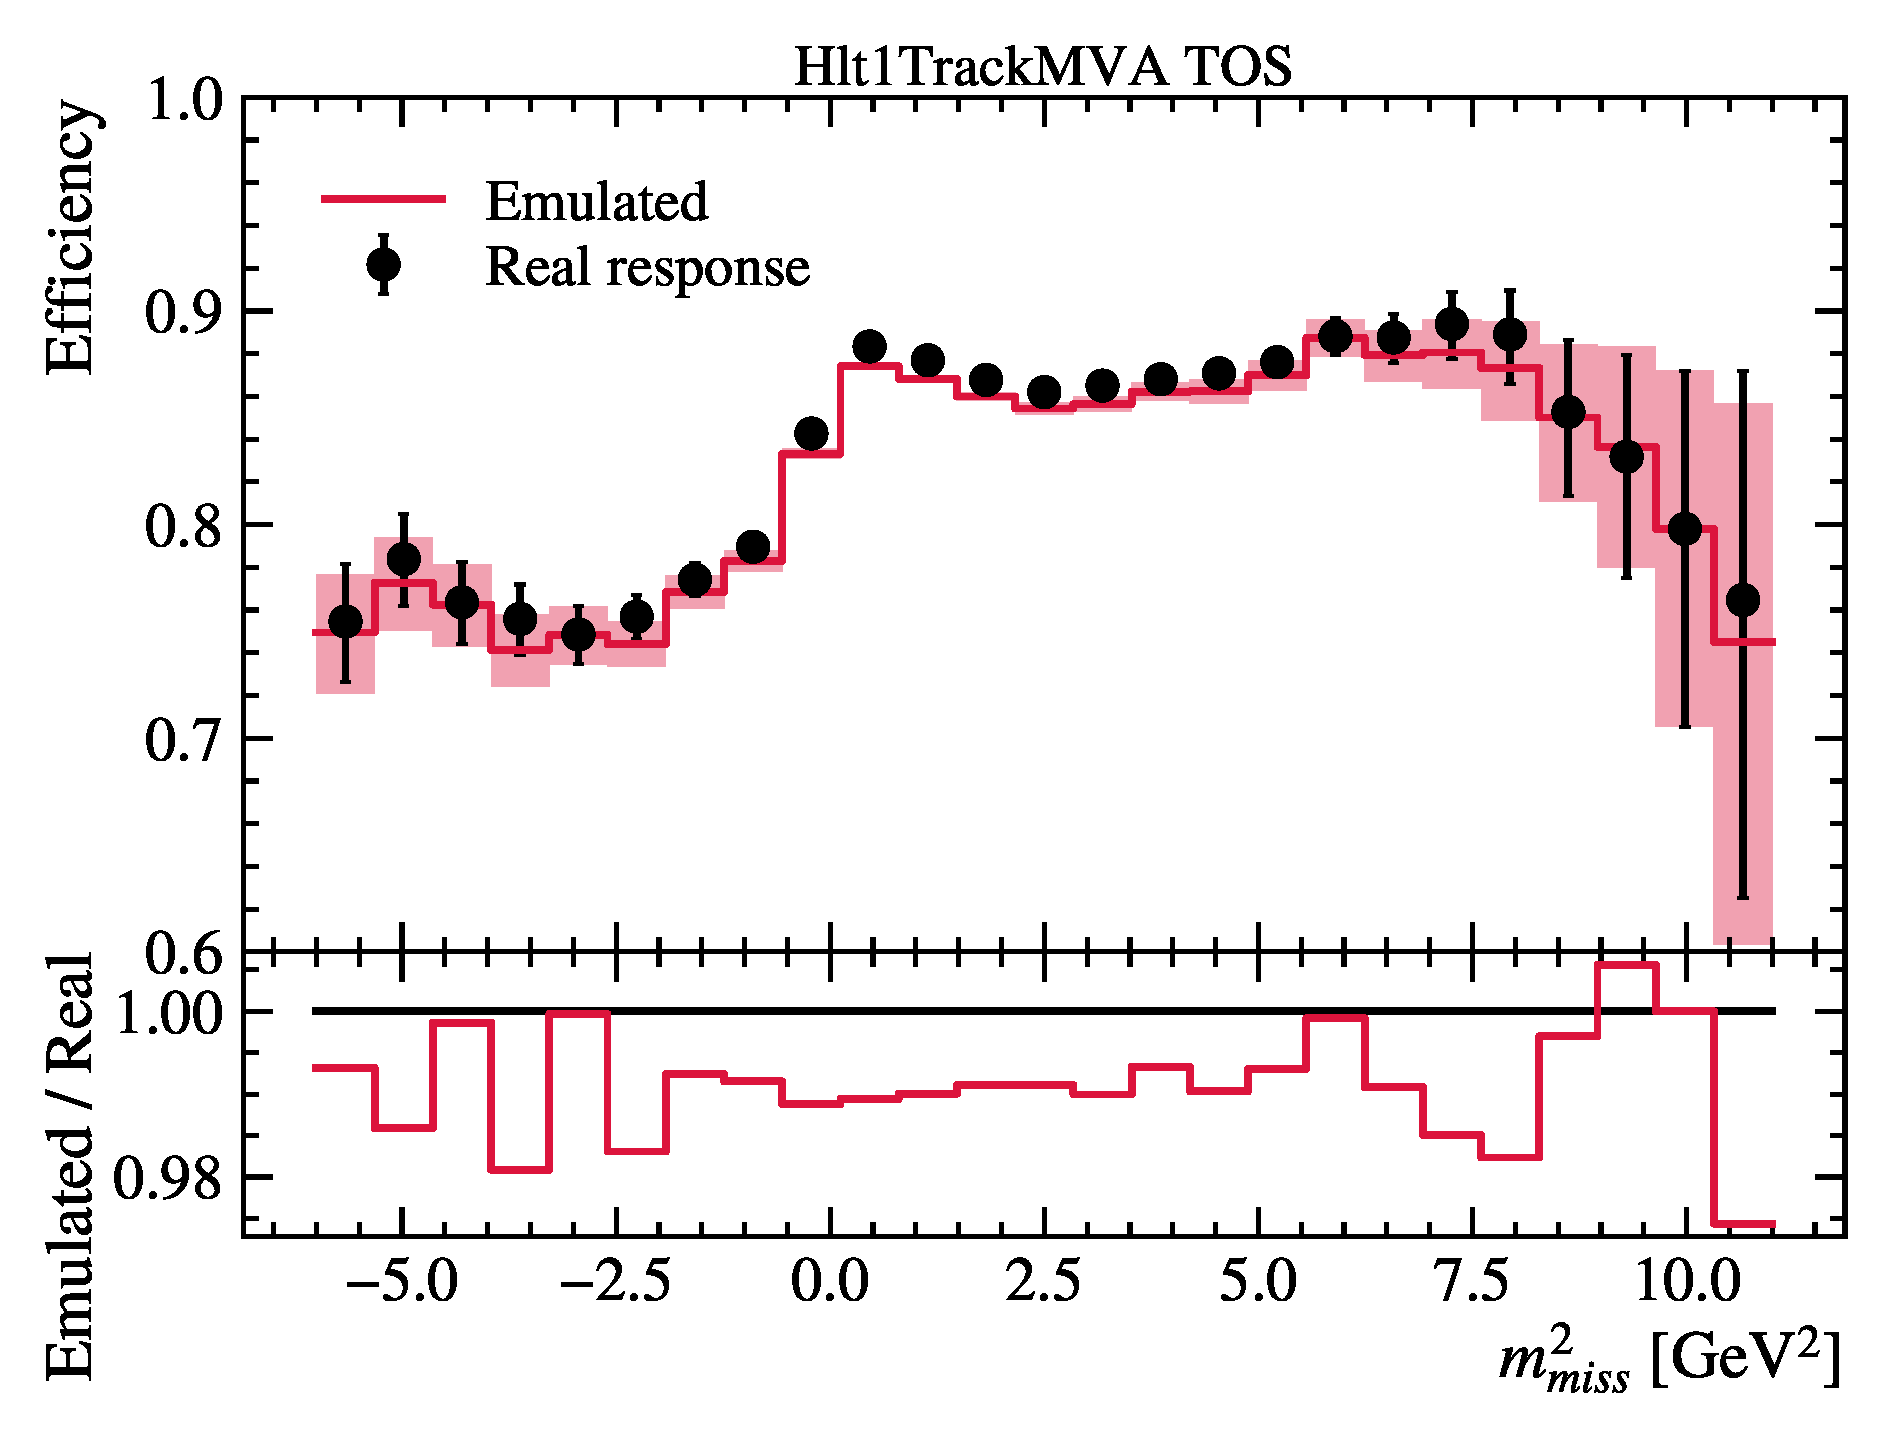
\includegraphics[width=0.32\textwidth]{
        ./figs-mc-emulation/emulate-hlt1/b_Hlt1TrackMVA_TOS_mmiss2.pdf
    }
    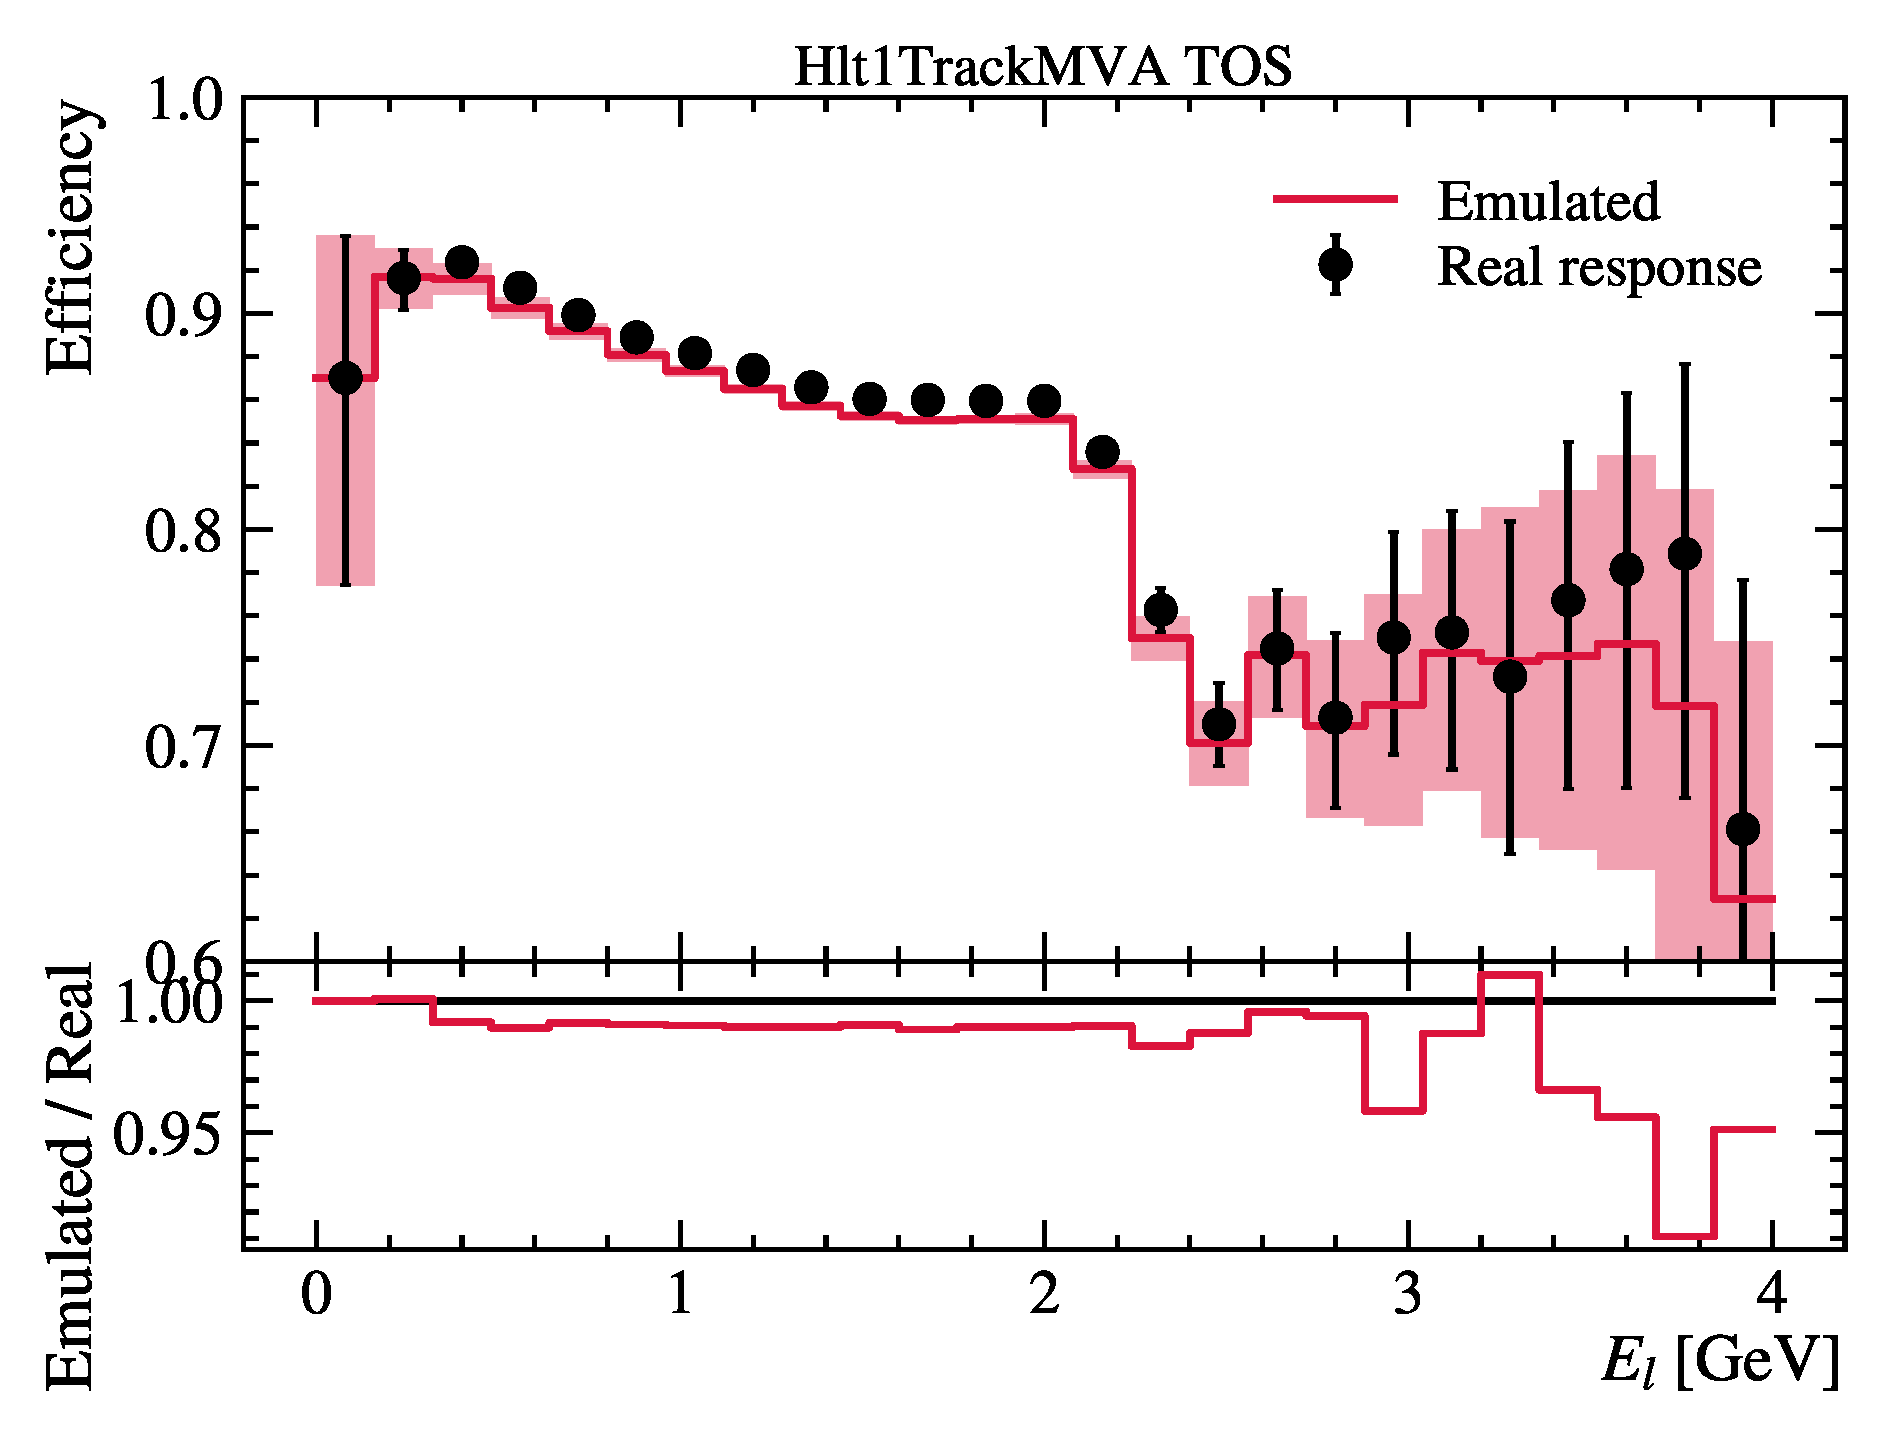
\includegraphics[width=0.32\textwidth]{
        ./figs-mc-emulation/emulate-hlt1/b_Hlt1TrackMVA_TOS_el.pdf
    }
    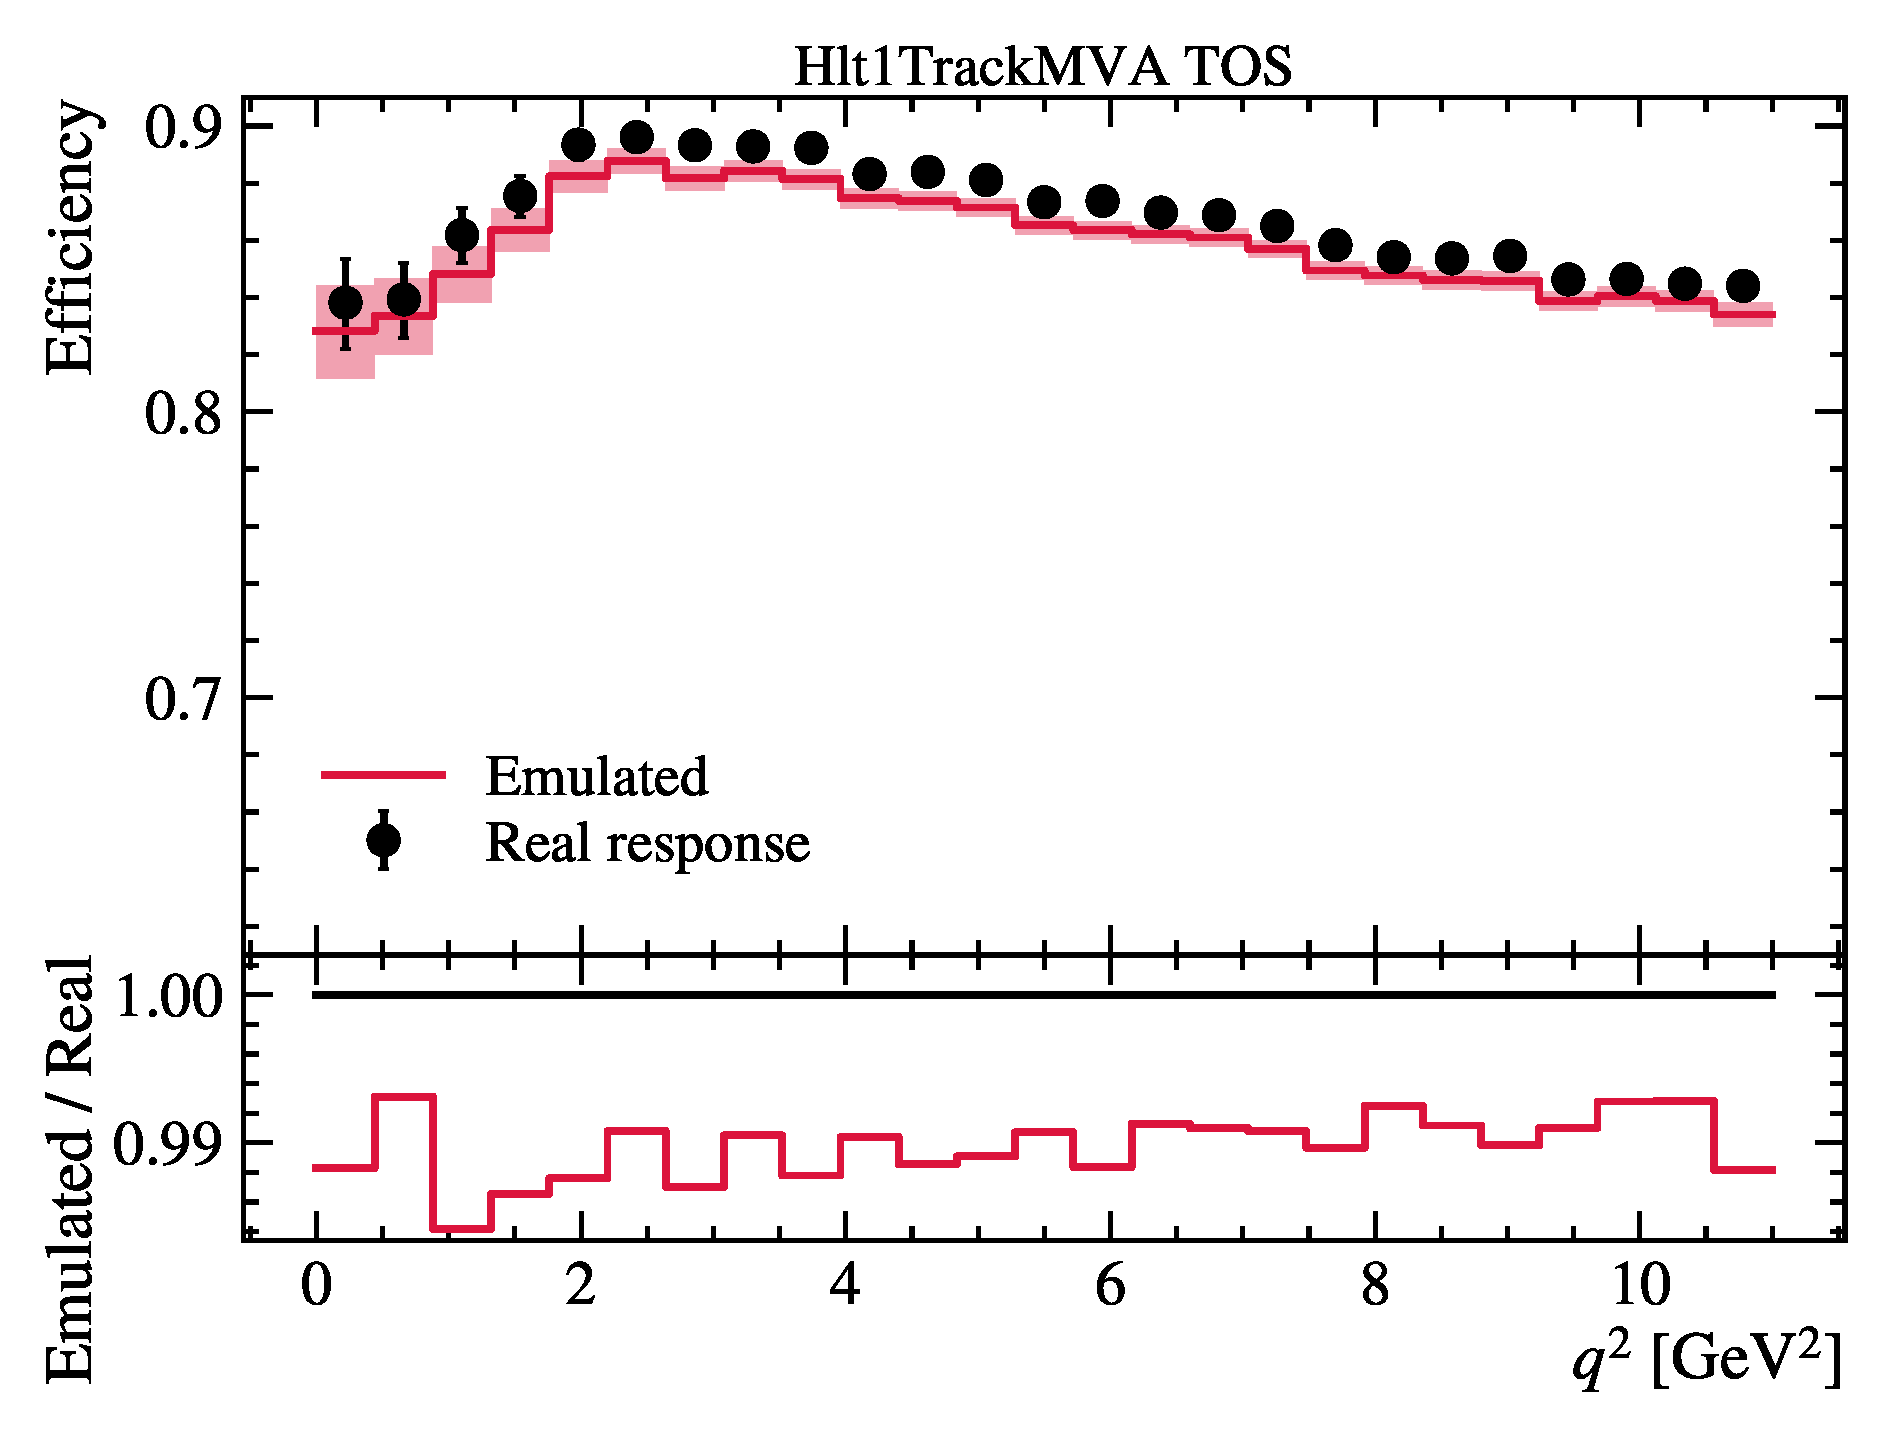
\includegraphics[width=0.32\textwidth]{
        ./figs-mc-emulation/emulate-hlt1/b_Hlt1TrackMVA_TOS_q2.pdf
    }

    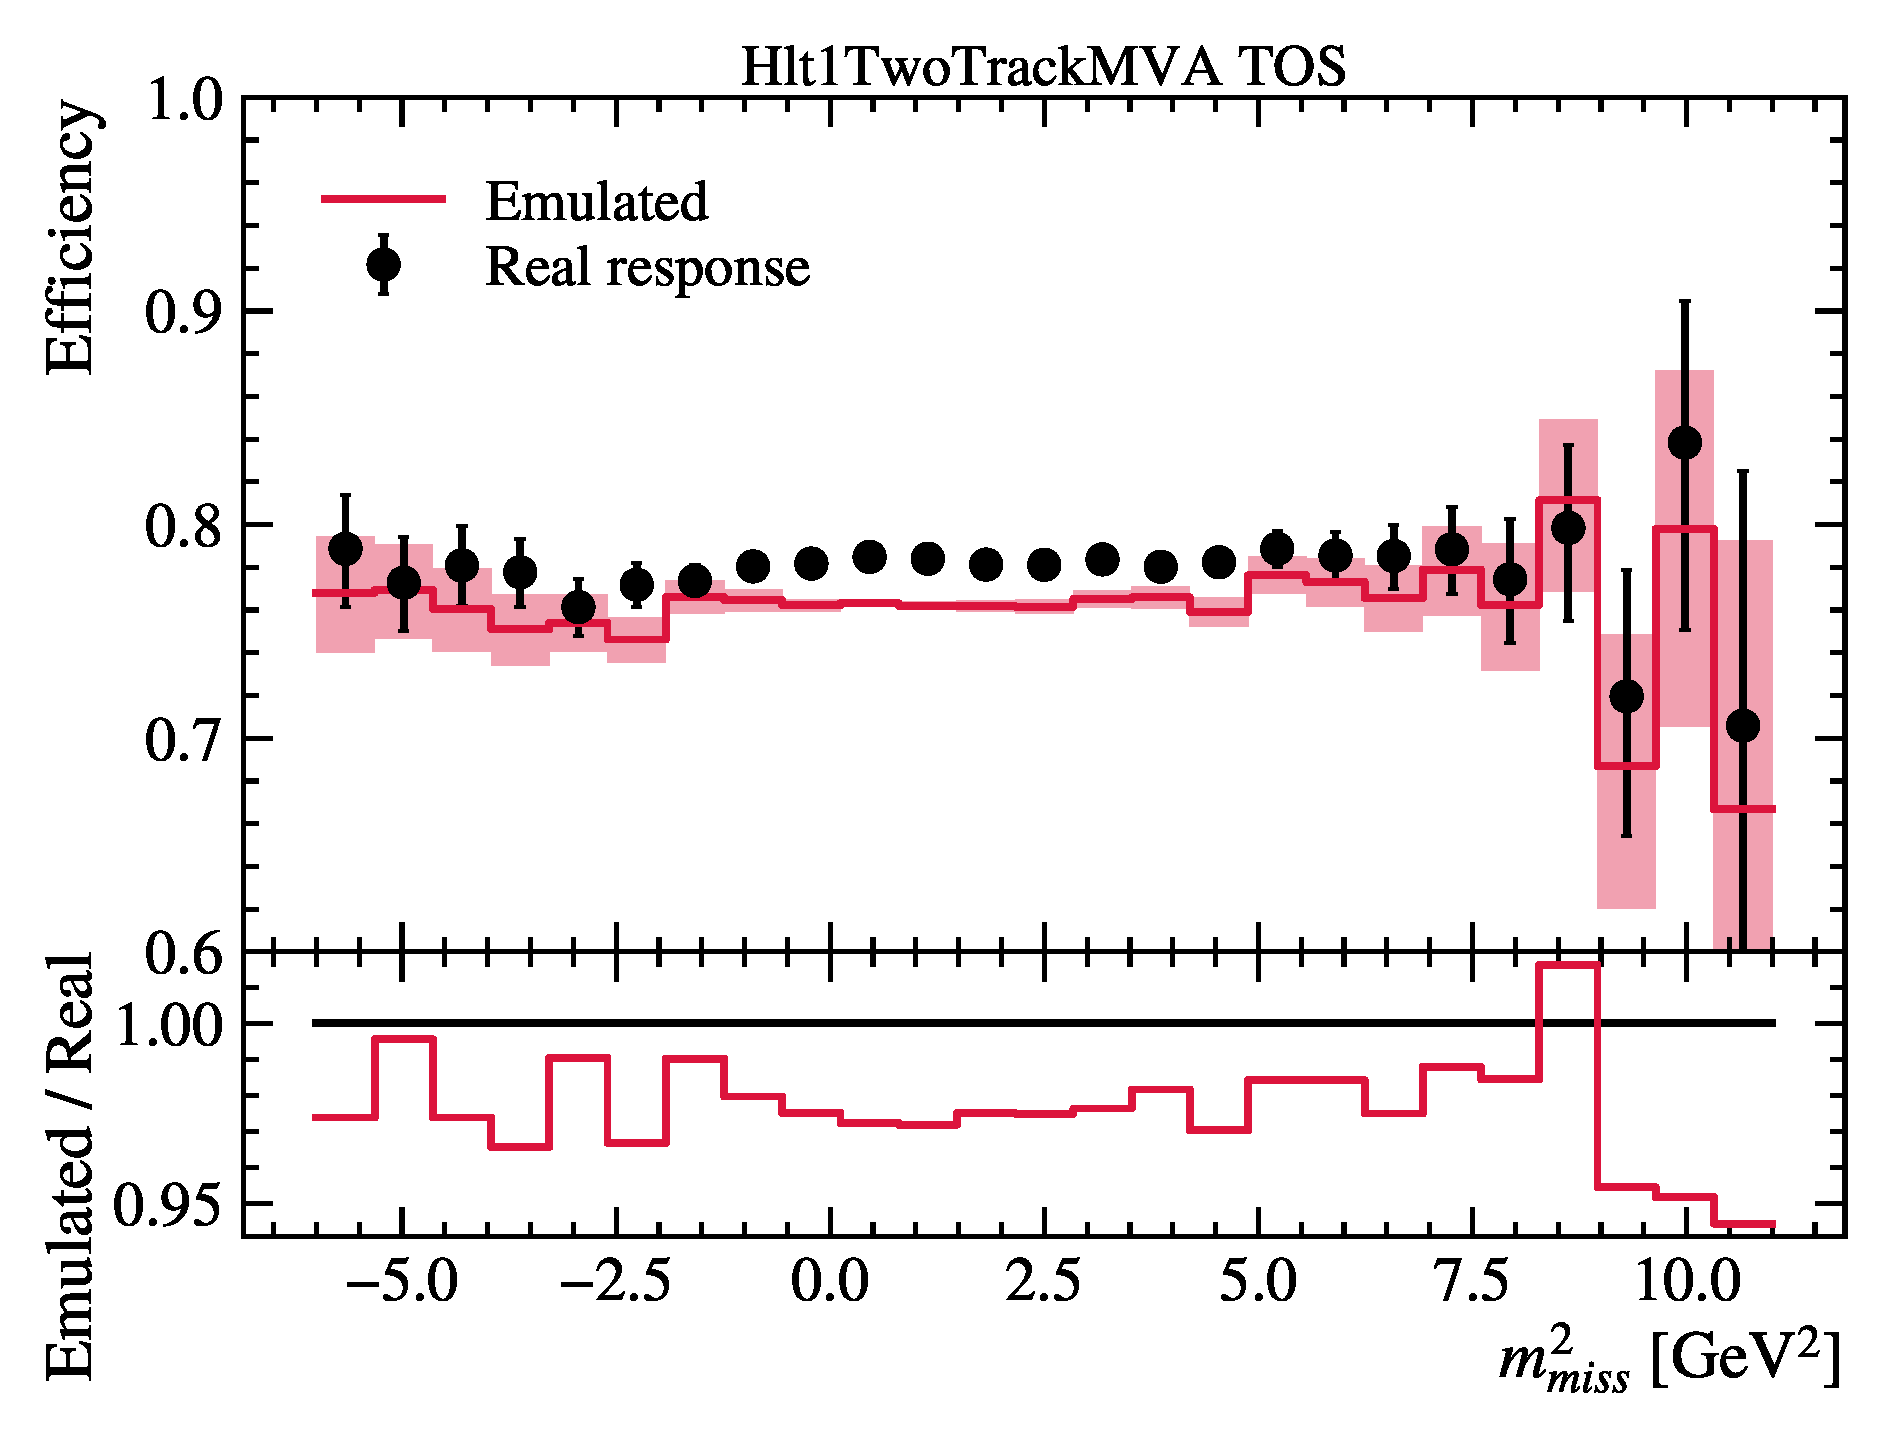
\includegraphics[width=0.32\textwidth]{
        ./figs-mc-emulation/emulate-hlt1/b_Hlt1TwoTrackMVA_TOS_mmiss2.pdf
    }
    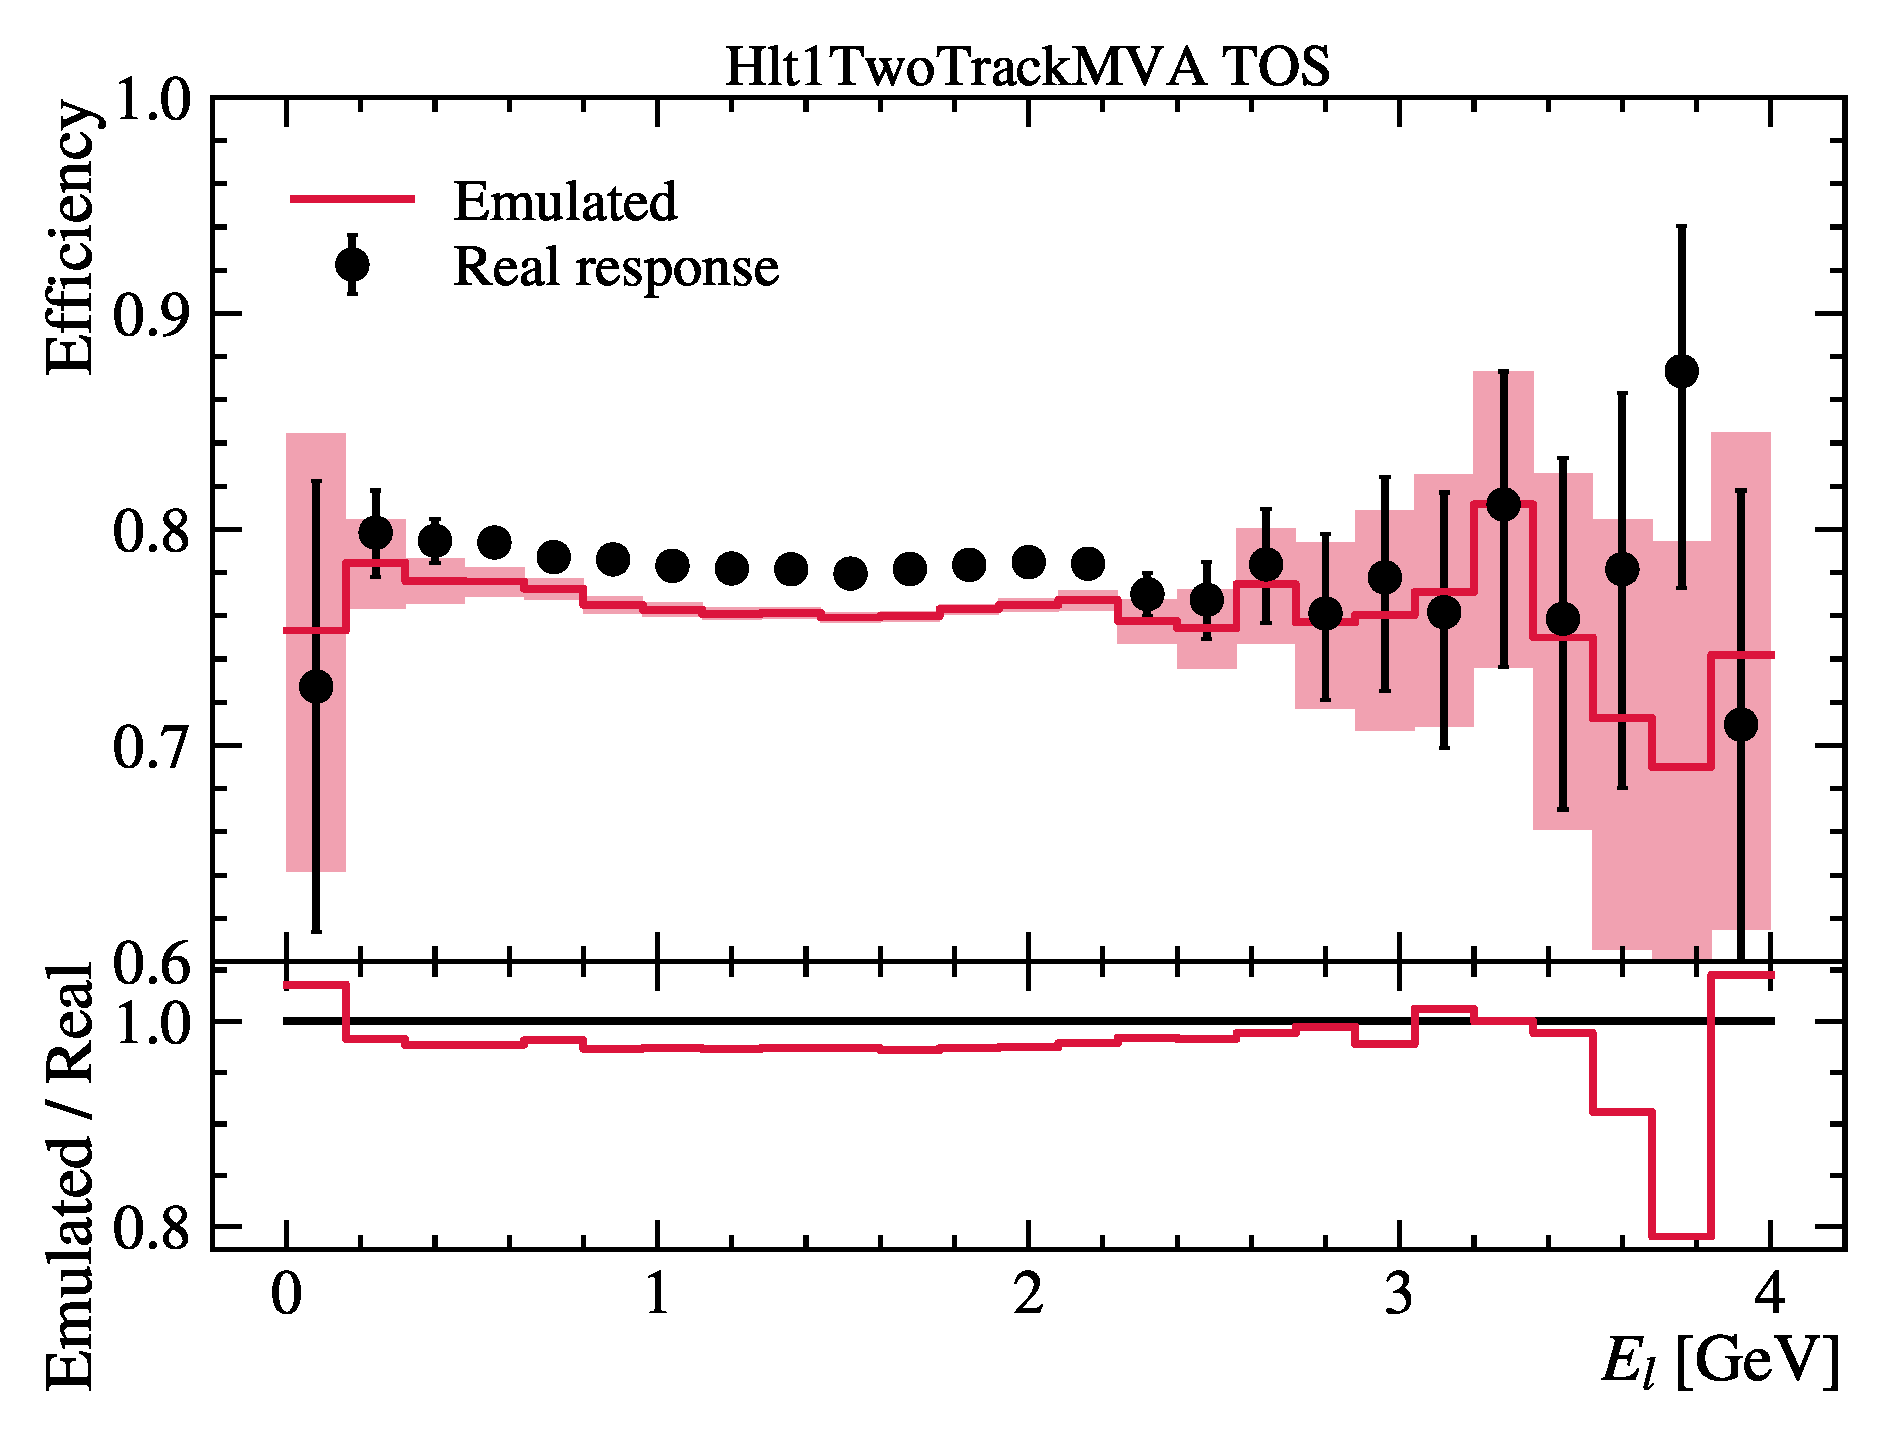
\includegraphics[width=0.32\textwidth]{
        ./figs-mc-emulation/emulate-hlt1/b_Hlt1TwoTrackMVA_TOS_el.pdf
    }
    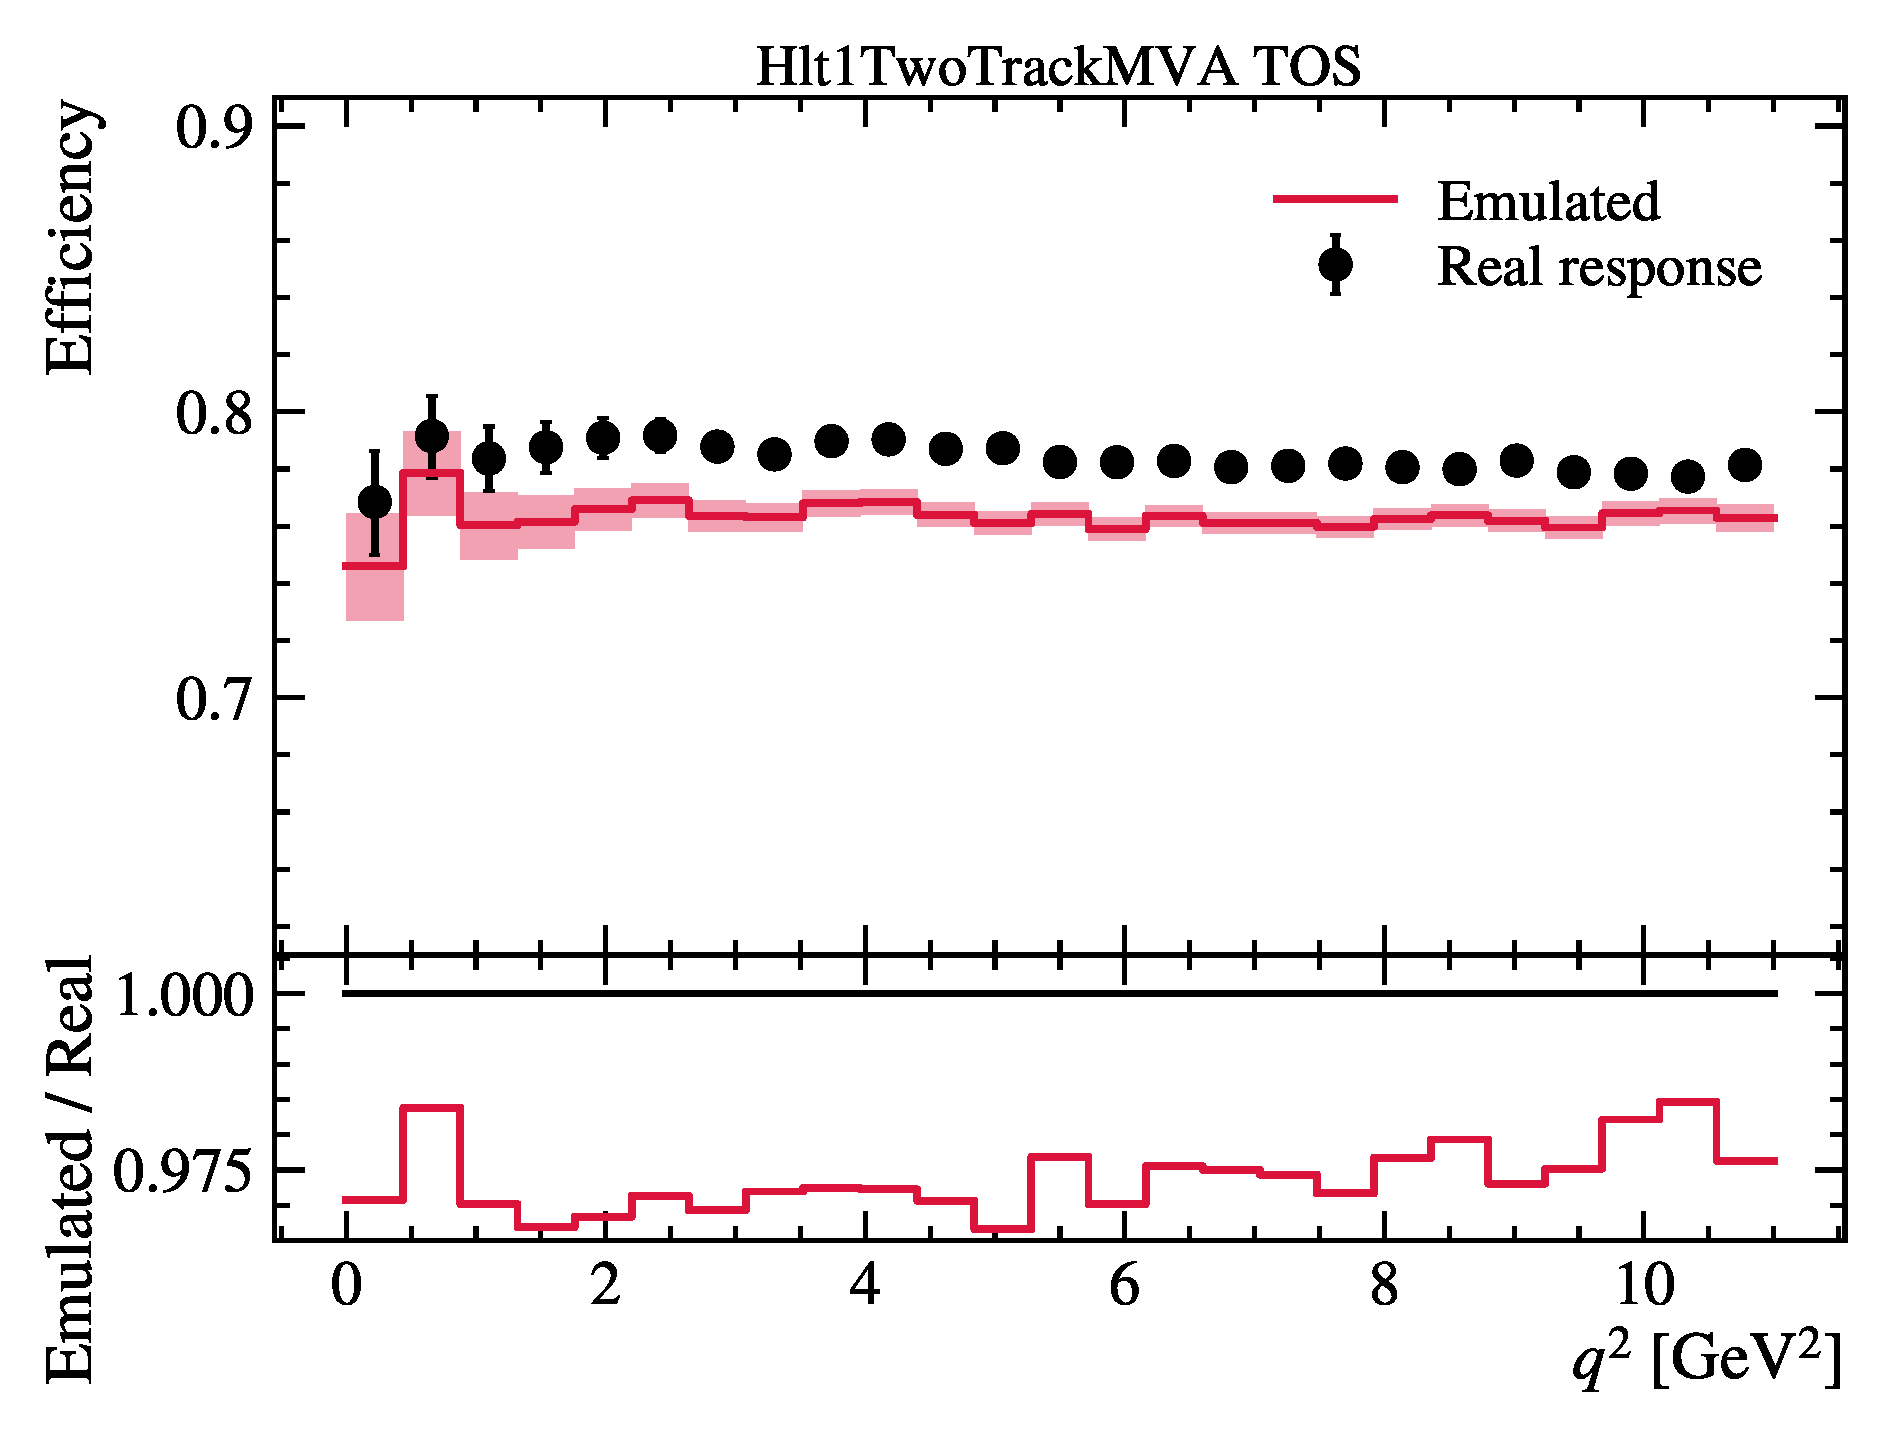
\includegraphics[width=0.32\textwidth]{
        ./figs-mc-emulation/emulate-hlt1/b_Hlt1TwoTrackMVA_TOS_q2.pdf
    }

    \caption{
        Emualted HLT1 triggers vs. real response in FullSim. For \Bp.
        The Hlt1TrackMVA agree very well, whereas Hlt1TwoTrackMVA still has a
        constant, albeit small ($\sim\!2.25$\%), discrepancy.
    }
    \label{fig:hlt1-trackmva-emu}
\end{figure}

\begin{figure}[ht]
    \centering
    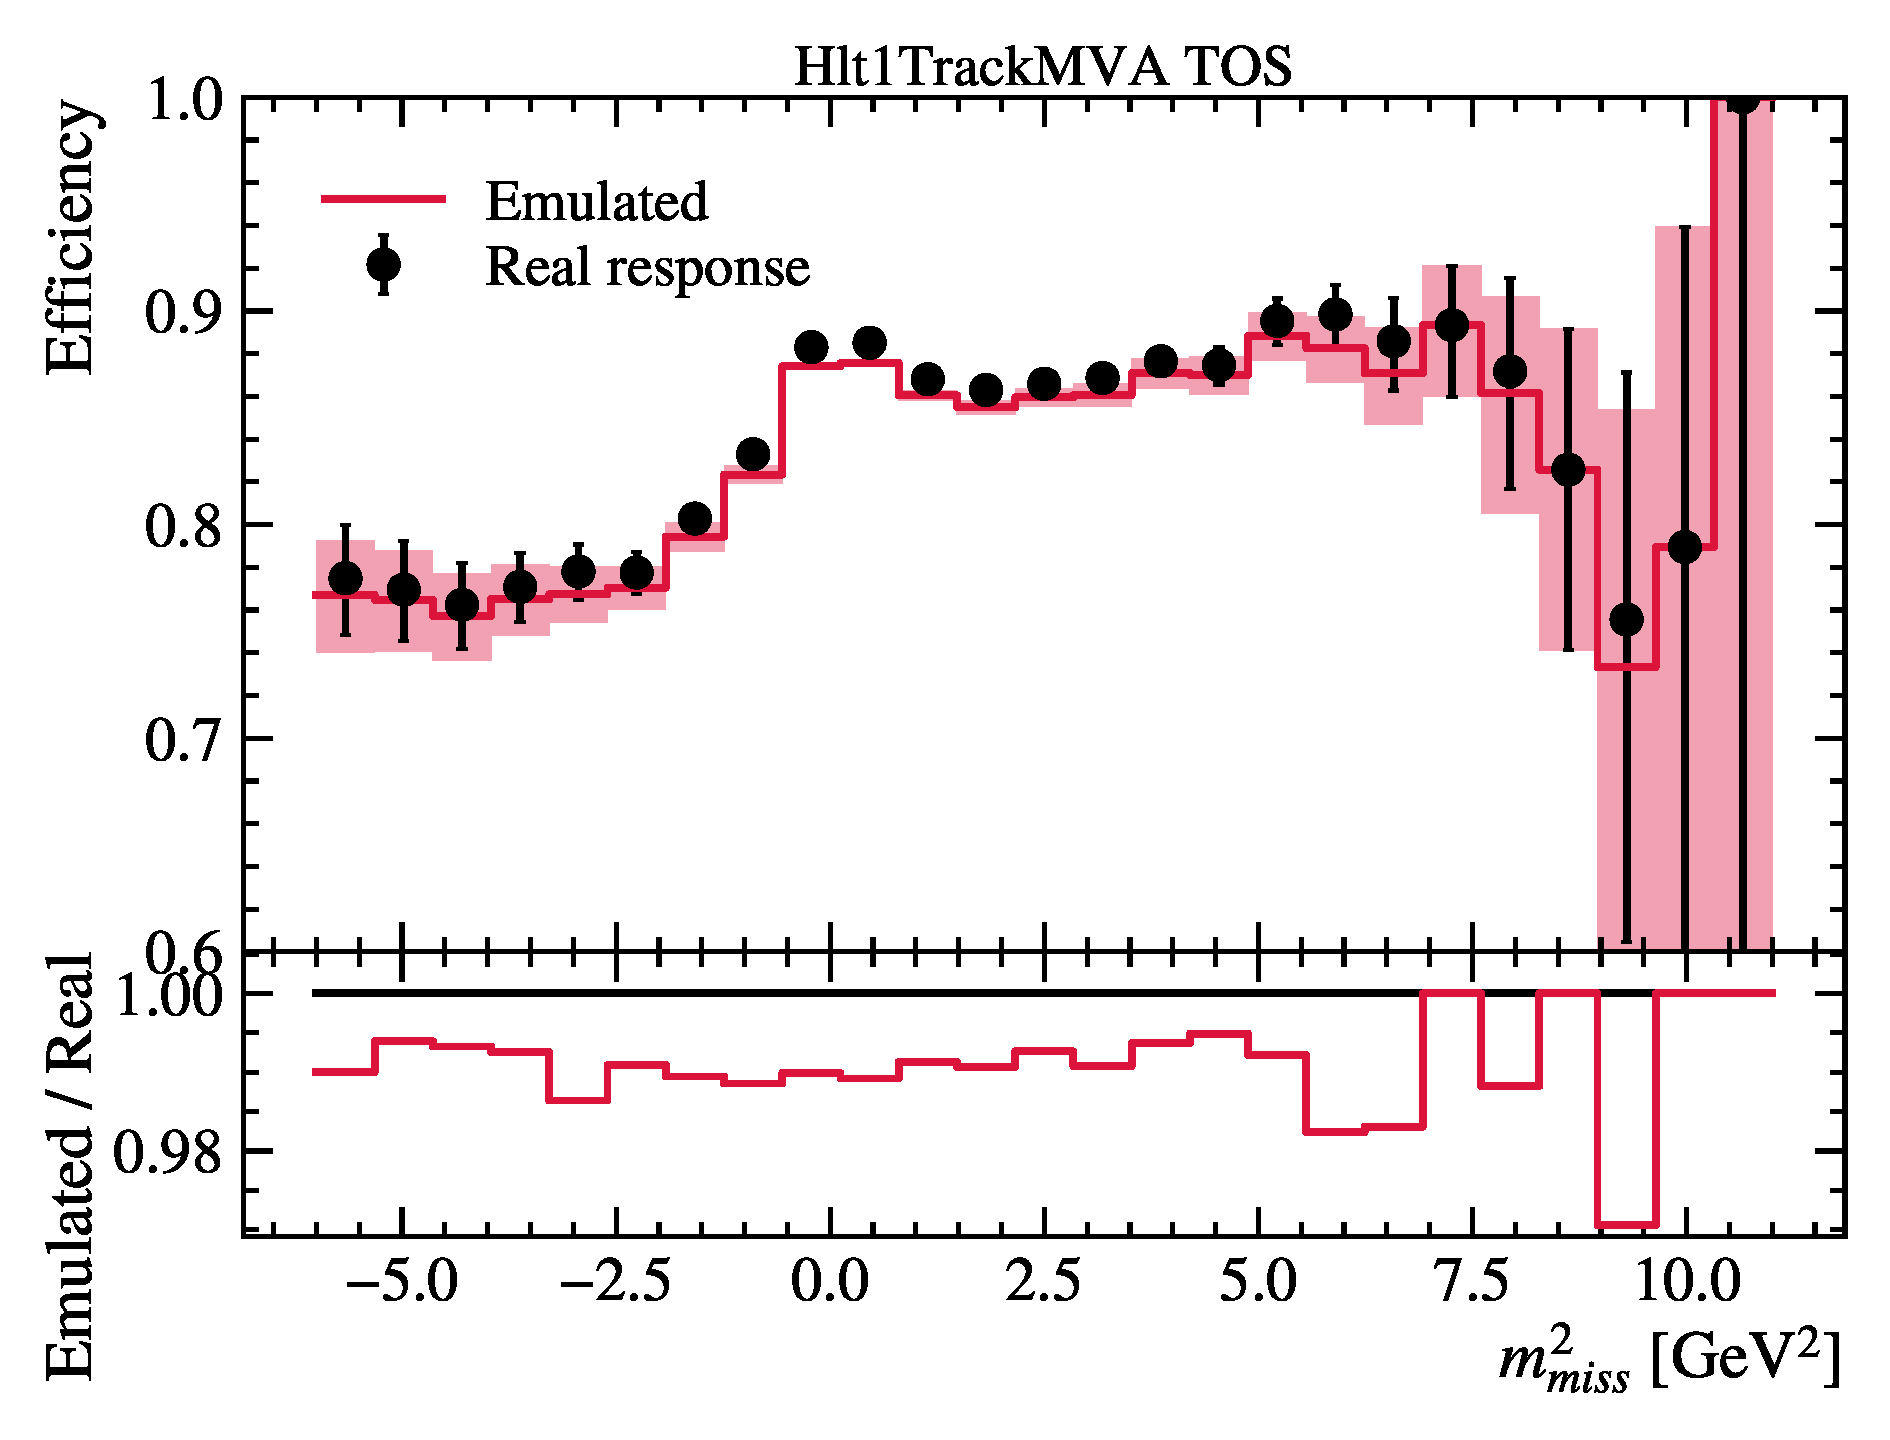
\includegraphics[width=0.32\textwidth]{
        ./figs-mc-emulation/emulate-hlt1/b0_Hlt1TrackMVA_TOS_mmiss2.pdf
    }
    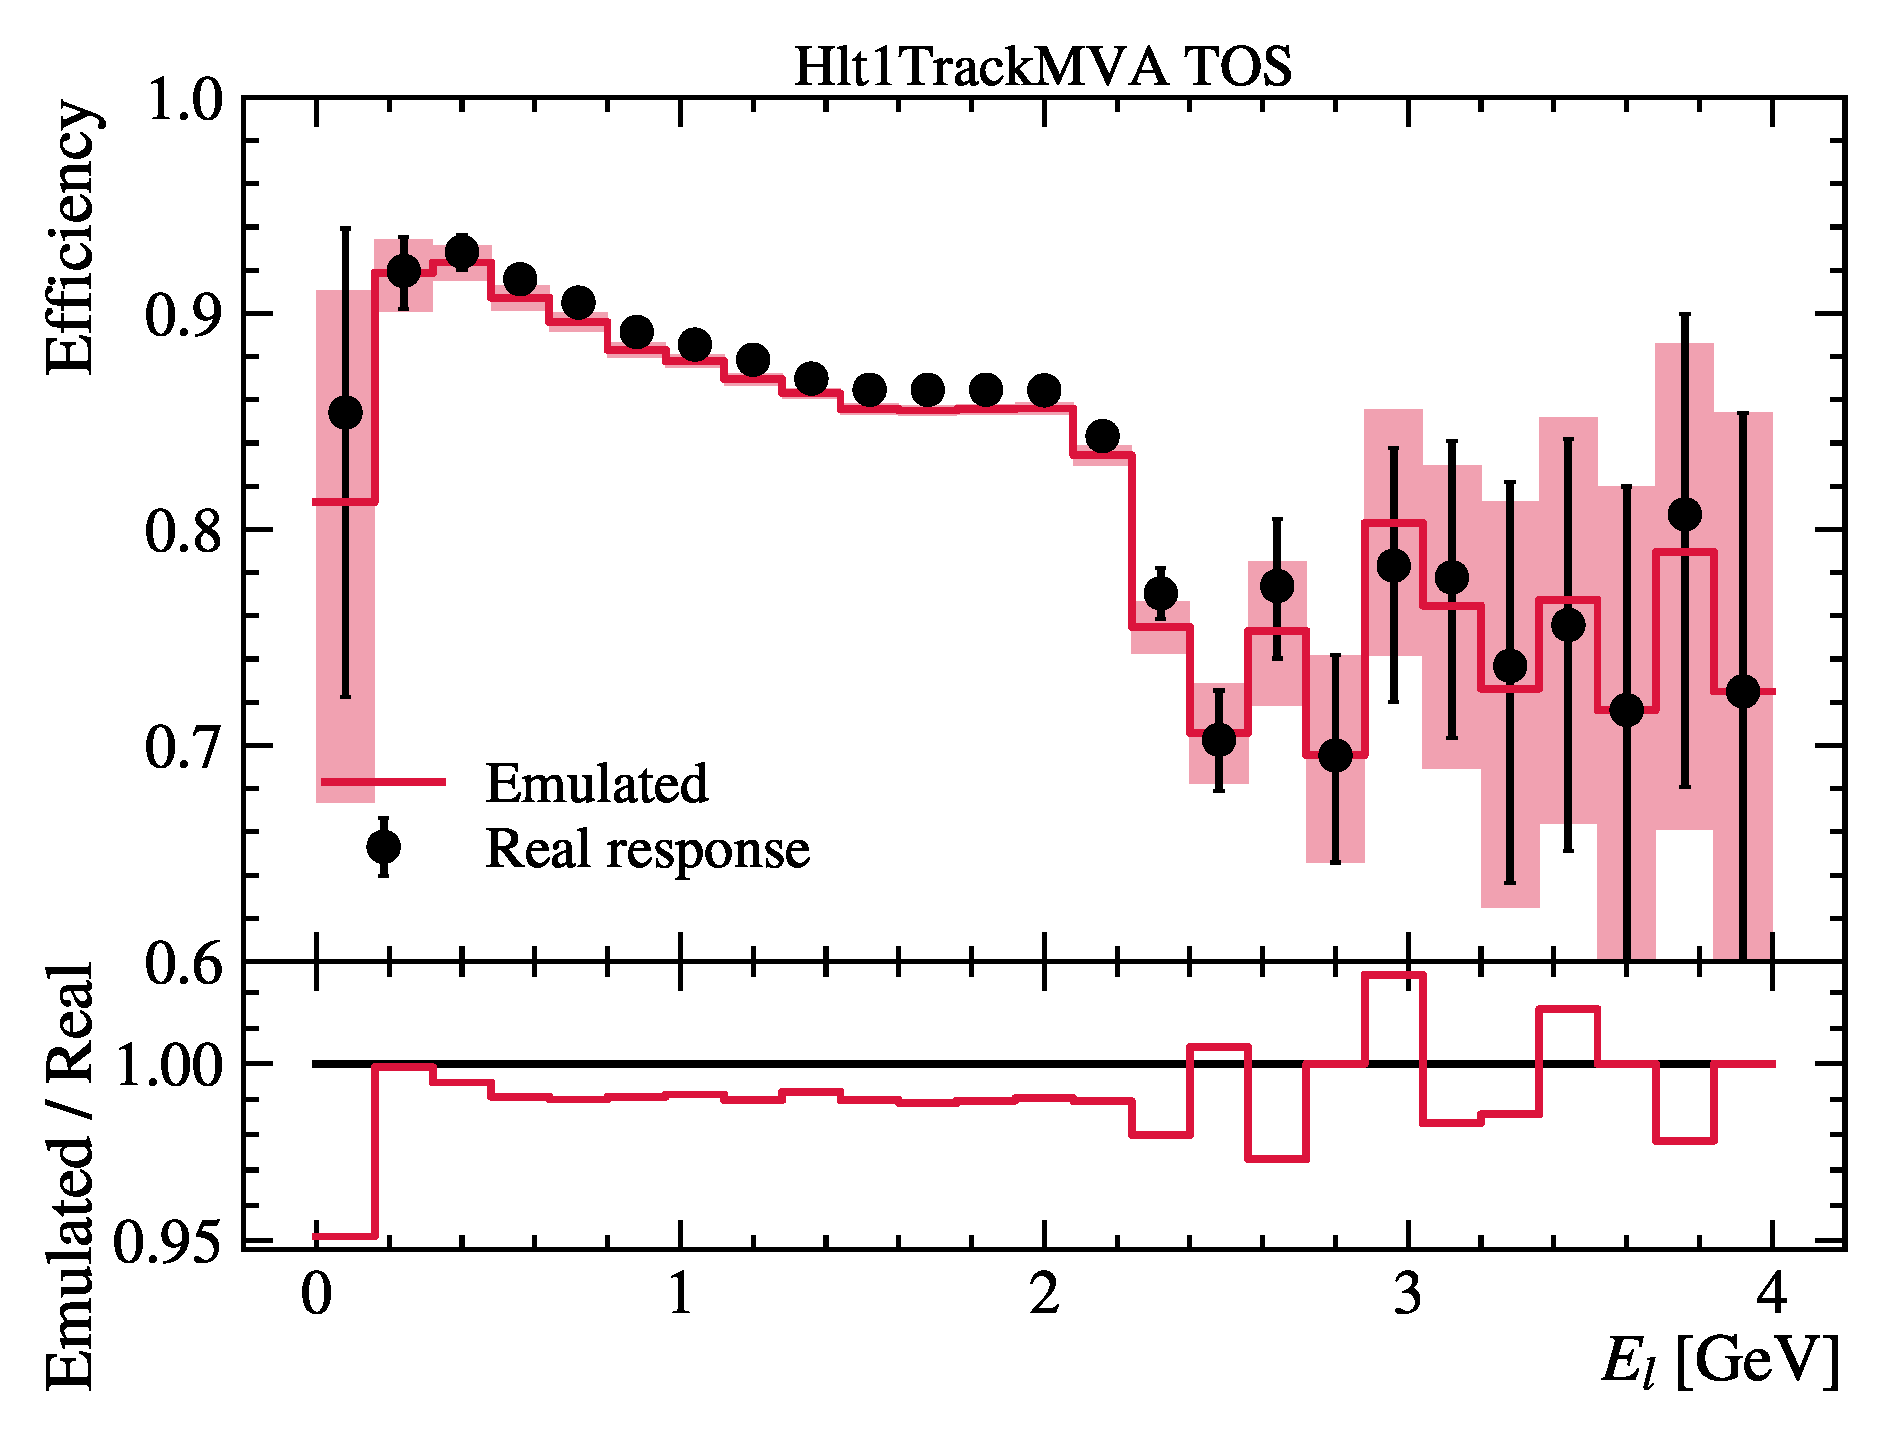
\includegraphics[width=0.32\textwidth]{
        ./figs-mc-emulation/emulate-hlt1/b0_Hlt1TrackMVA_TOS_el.pdf
    }
    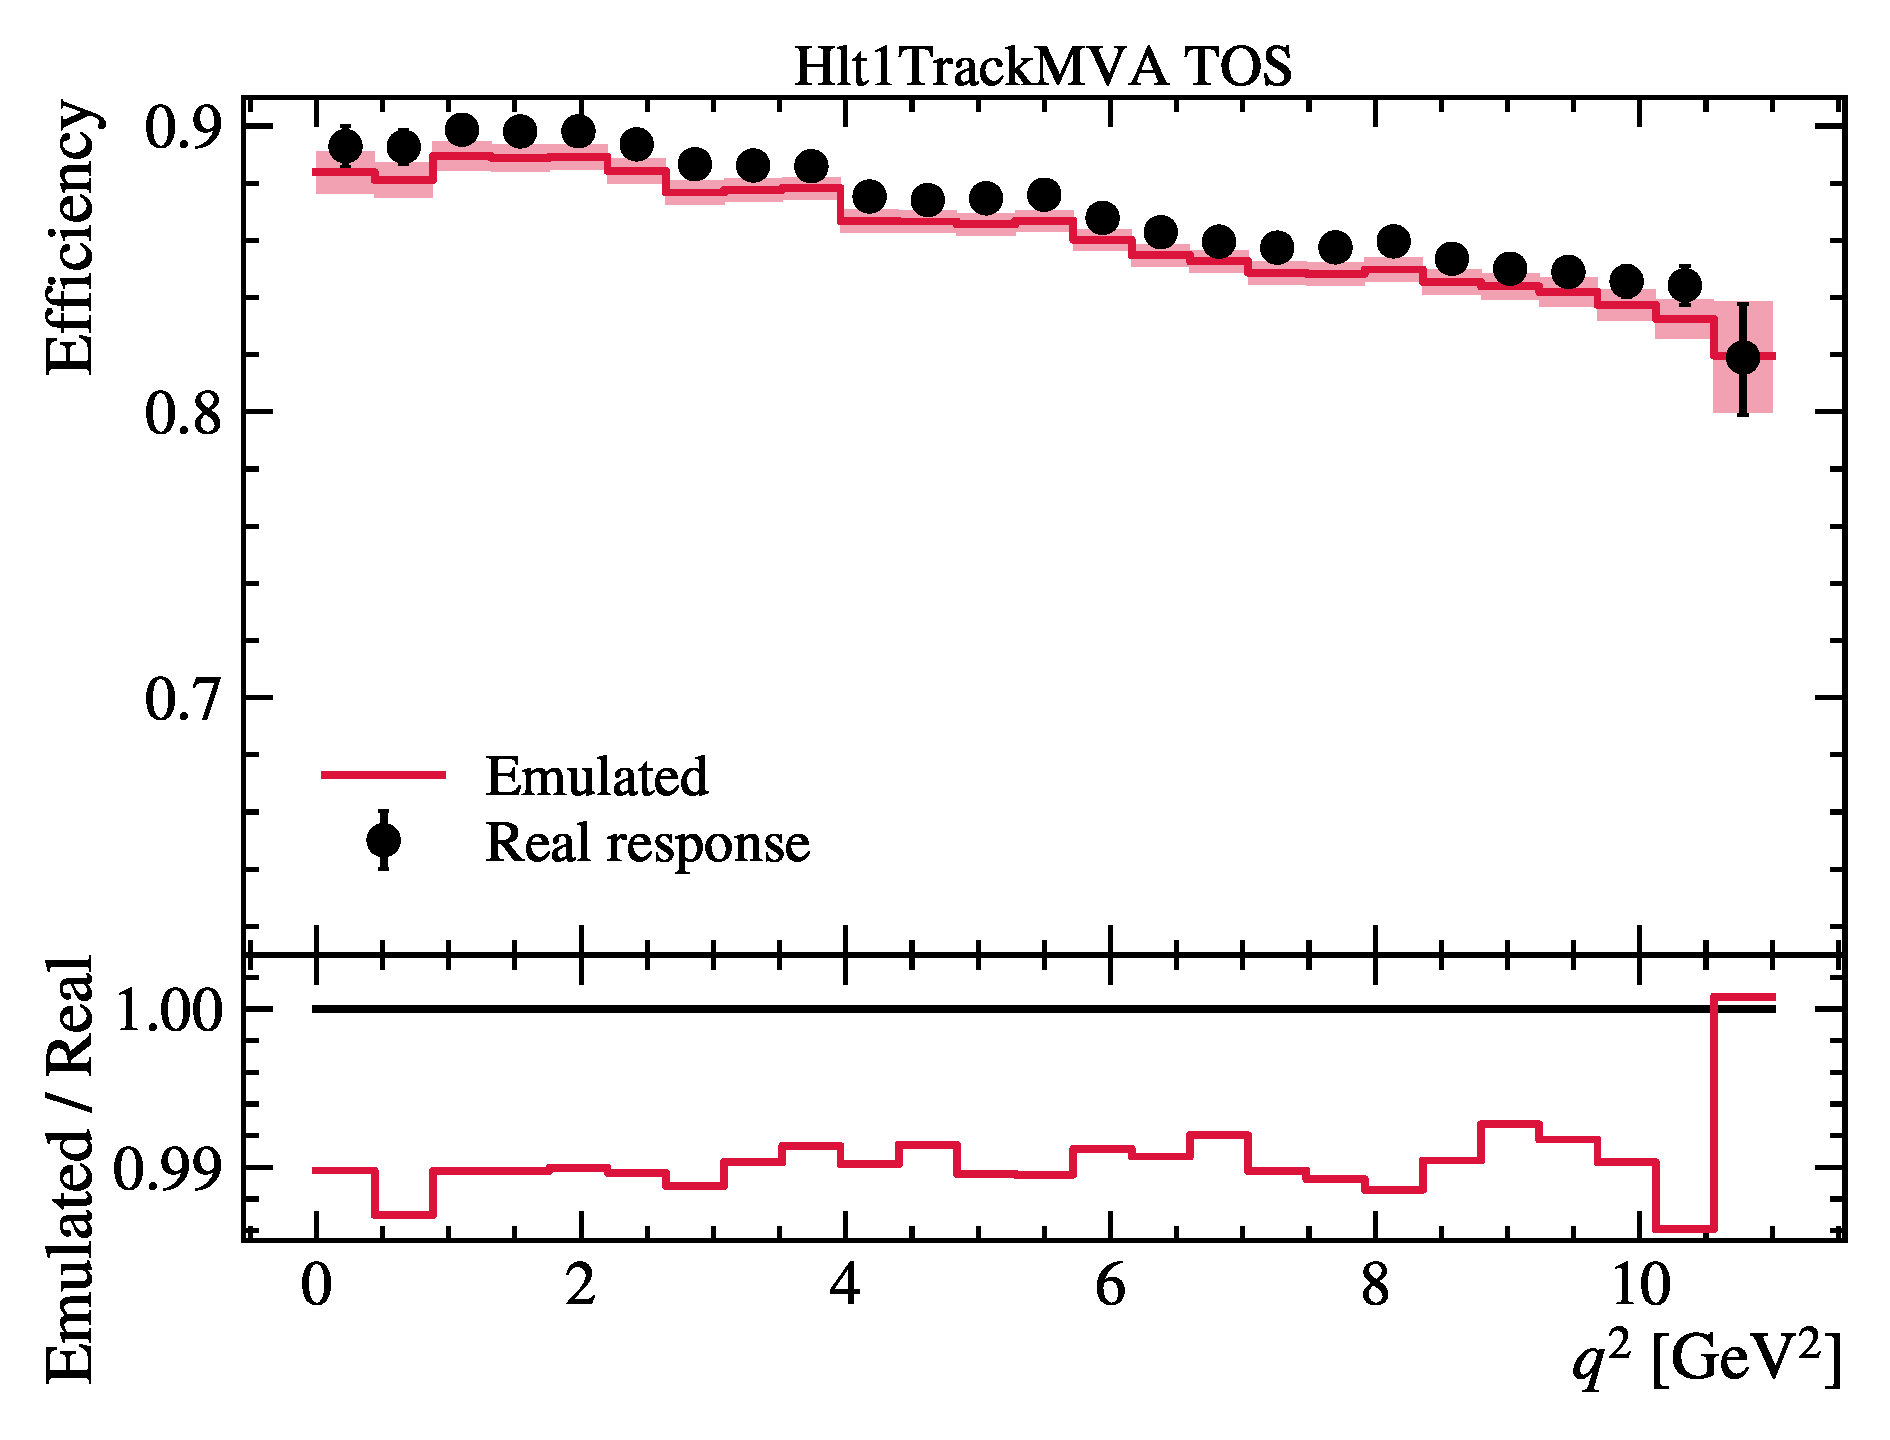
\includegraphics[width=0.32\textwidth]{
        ./figs-mc-emulation/emulate-hlt1/b0_Hlt1TrackMVA_TOS_q2.pdf
    }

    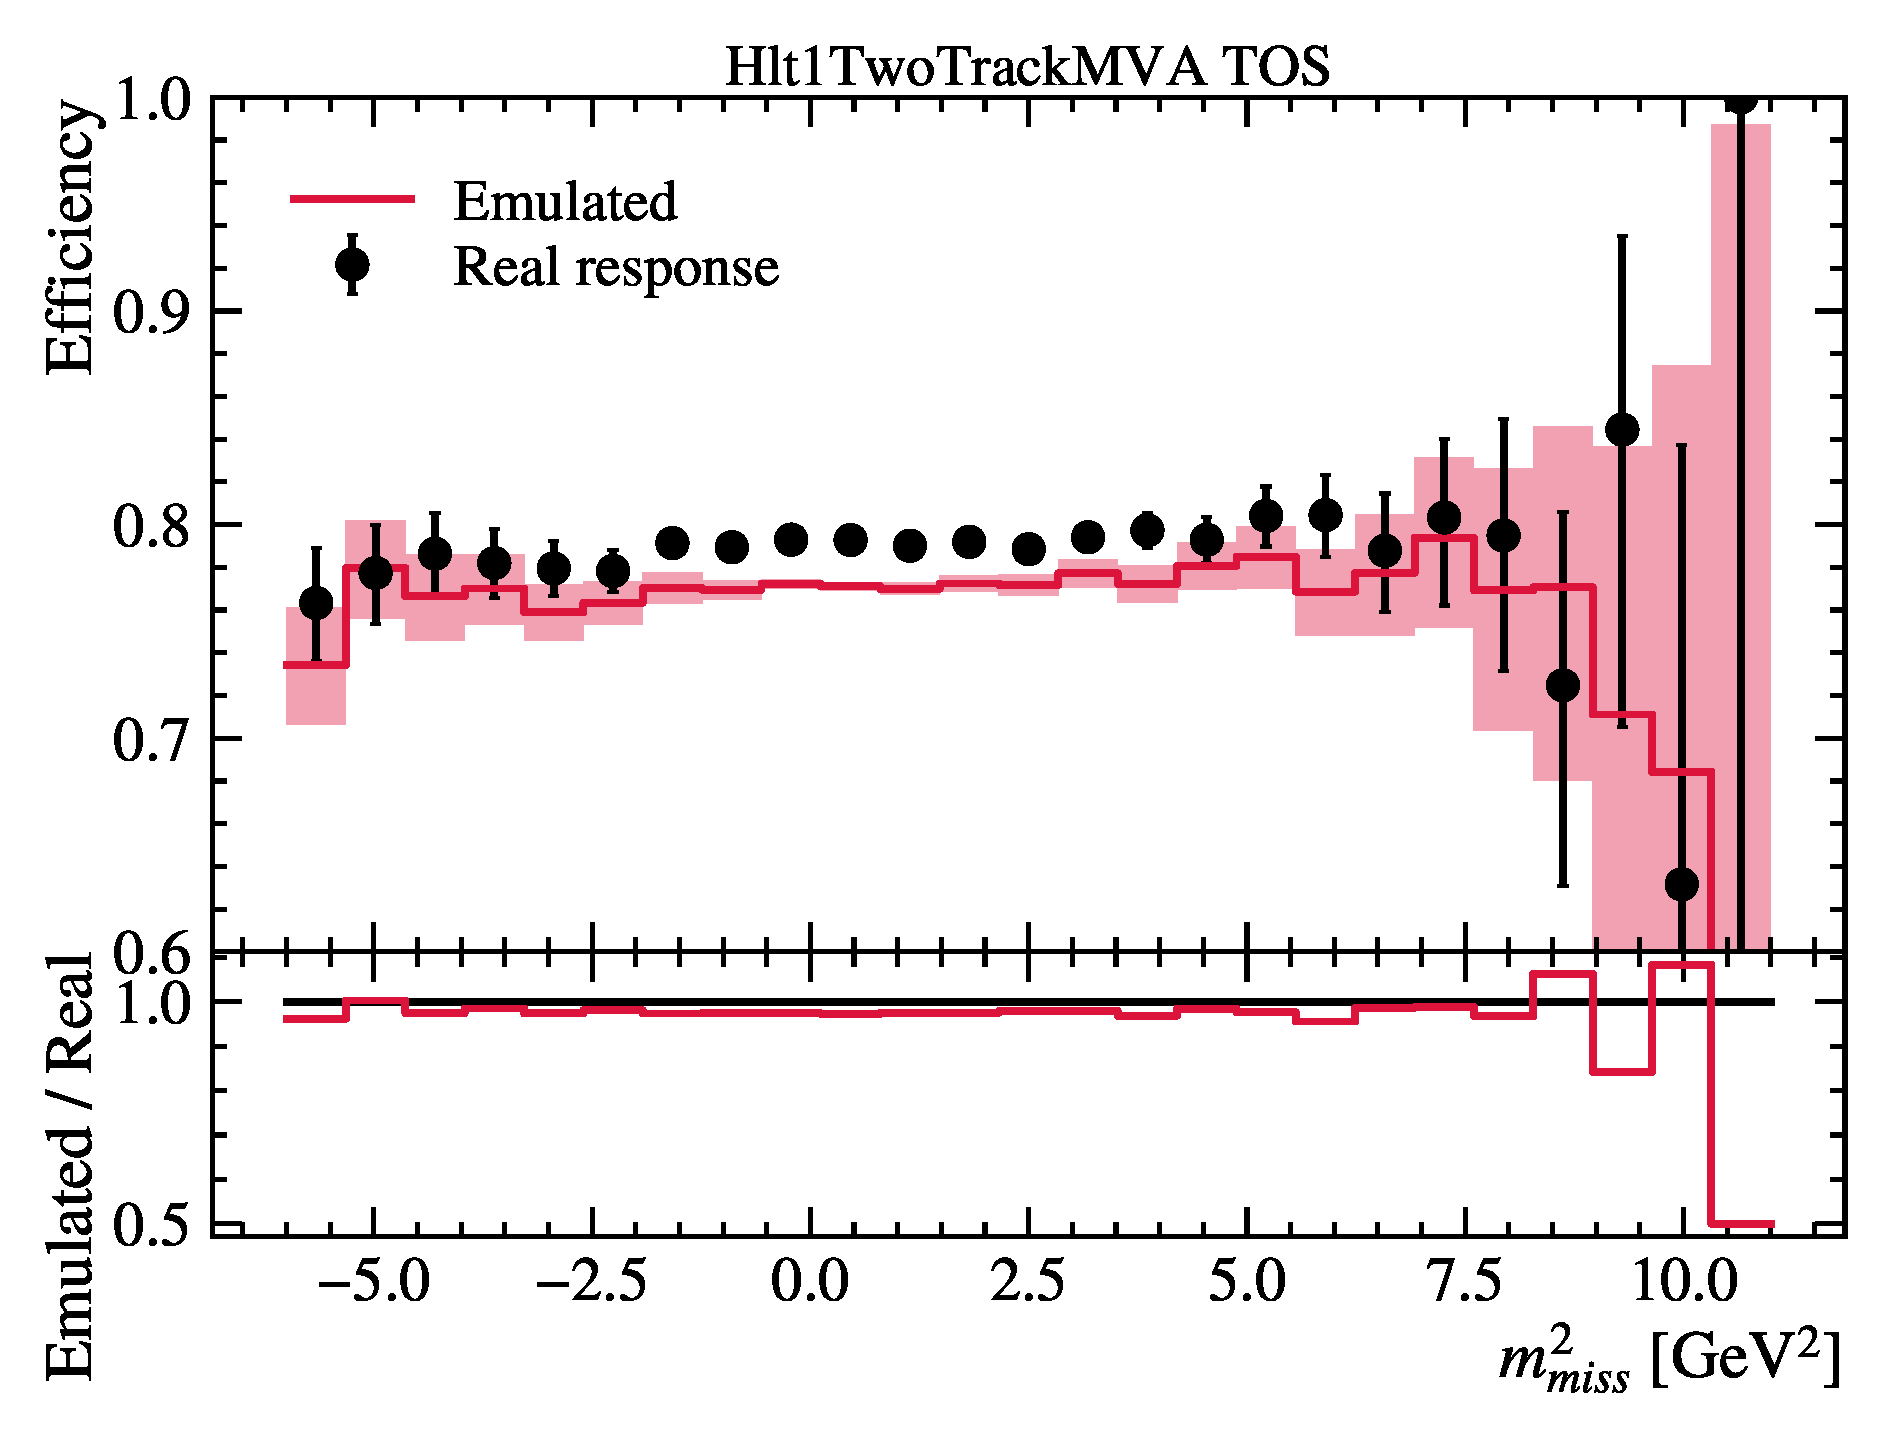
\includegraphics[width=0.32\textwidth]{
        ./figs-mc-emulation/emulate-hlt1/b0_Hlt1TwoTrackMVA_TOS_mmiss2.pdf
    }
    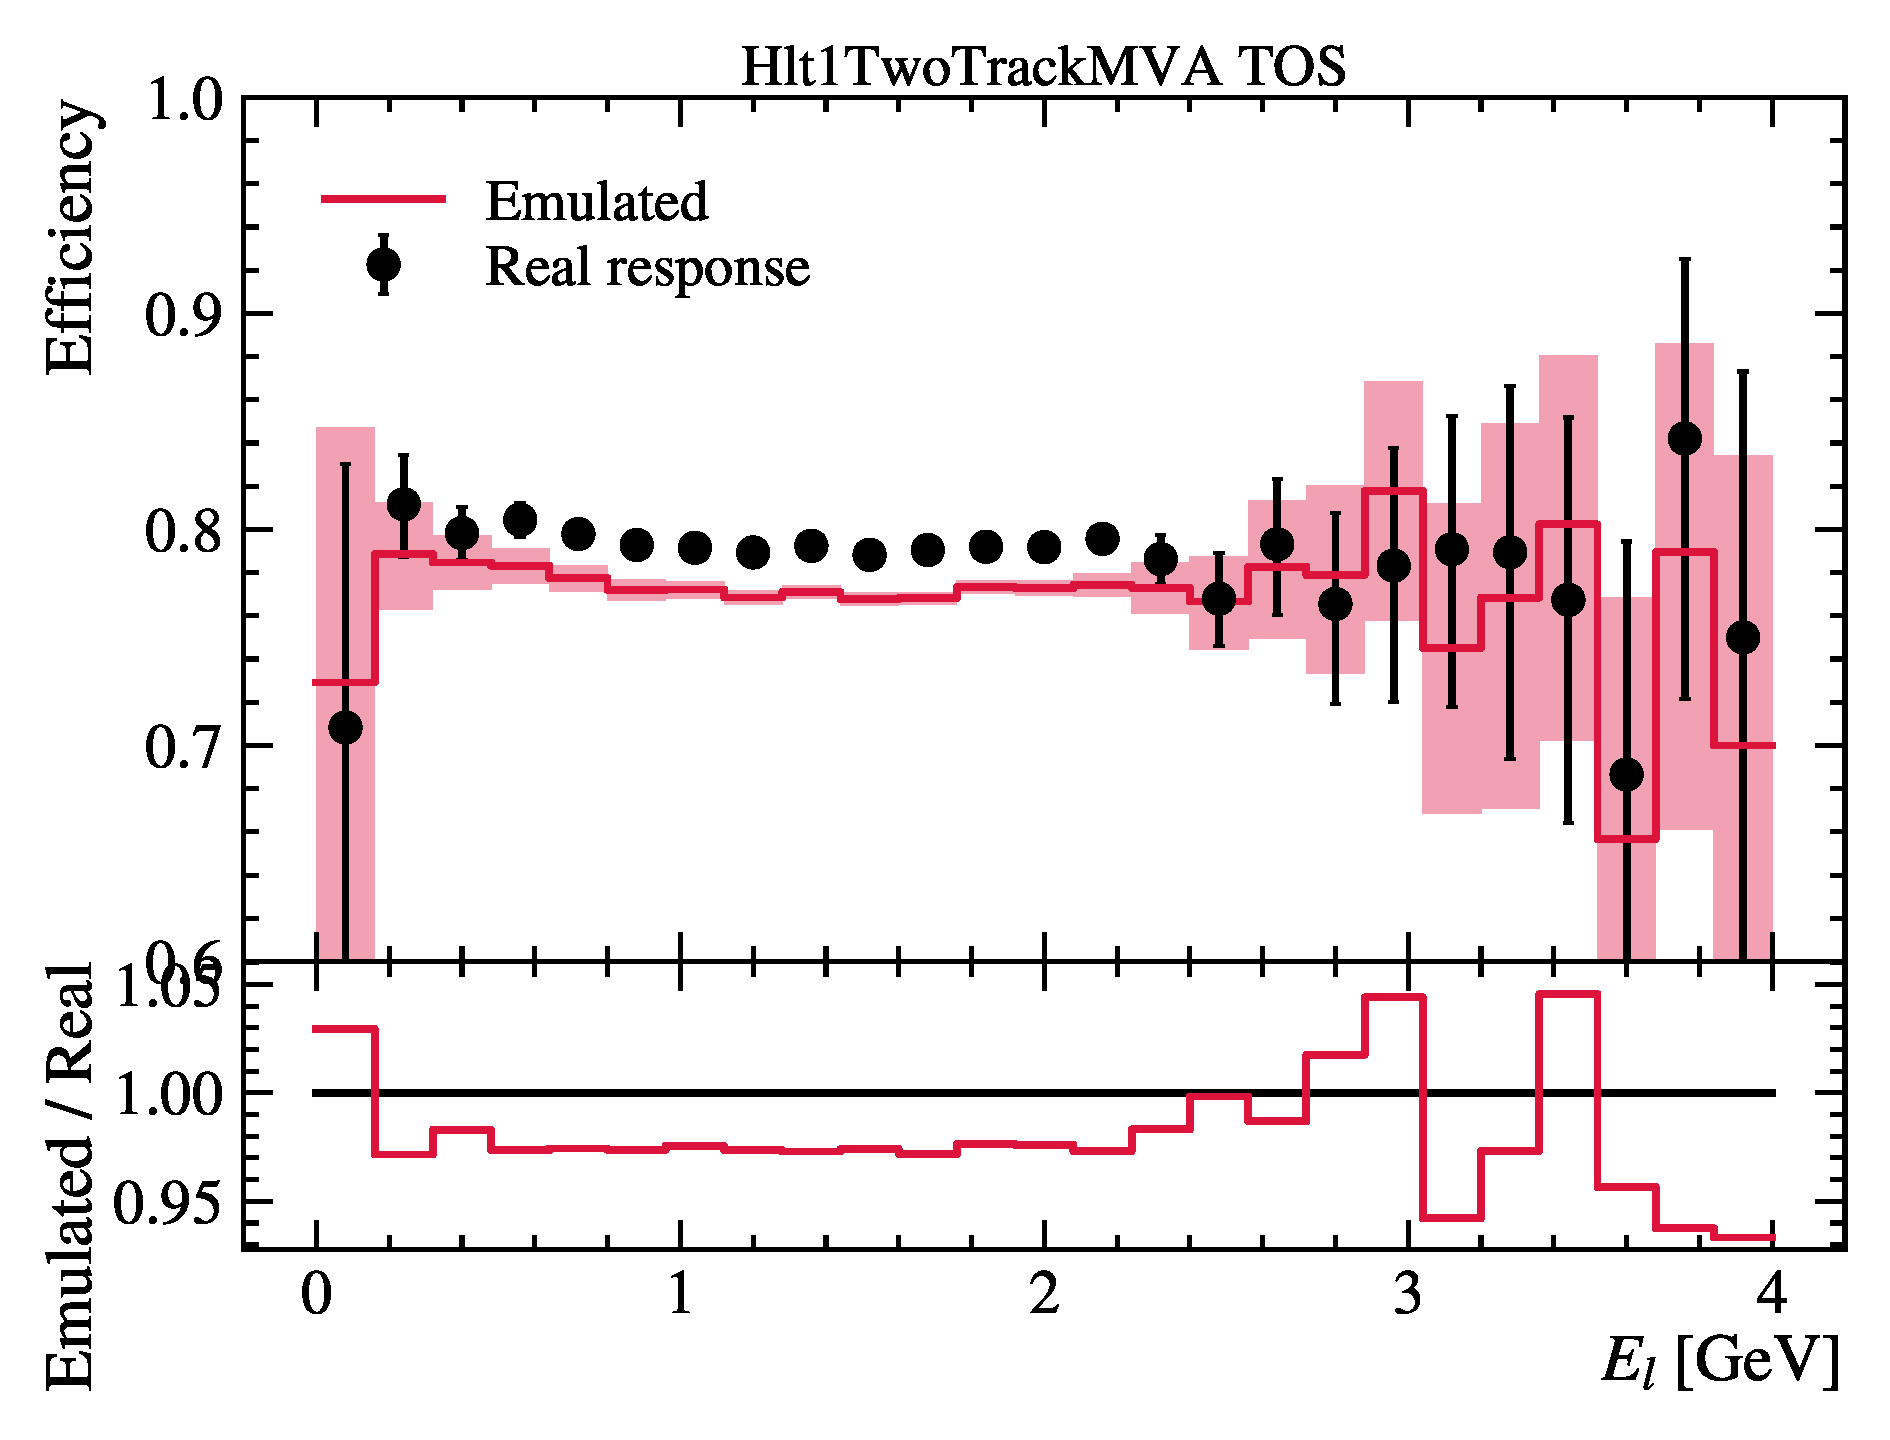
\includegraphics[width=0.32\textwidth]{
        ./figs-mc-emulation/emulate-hlt1/b0_Hlt1TwoTrackMVA_TOS_el.pdf
    }
    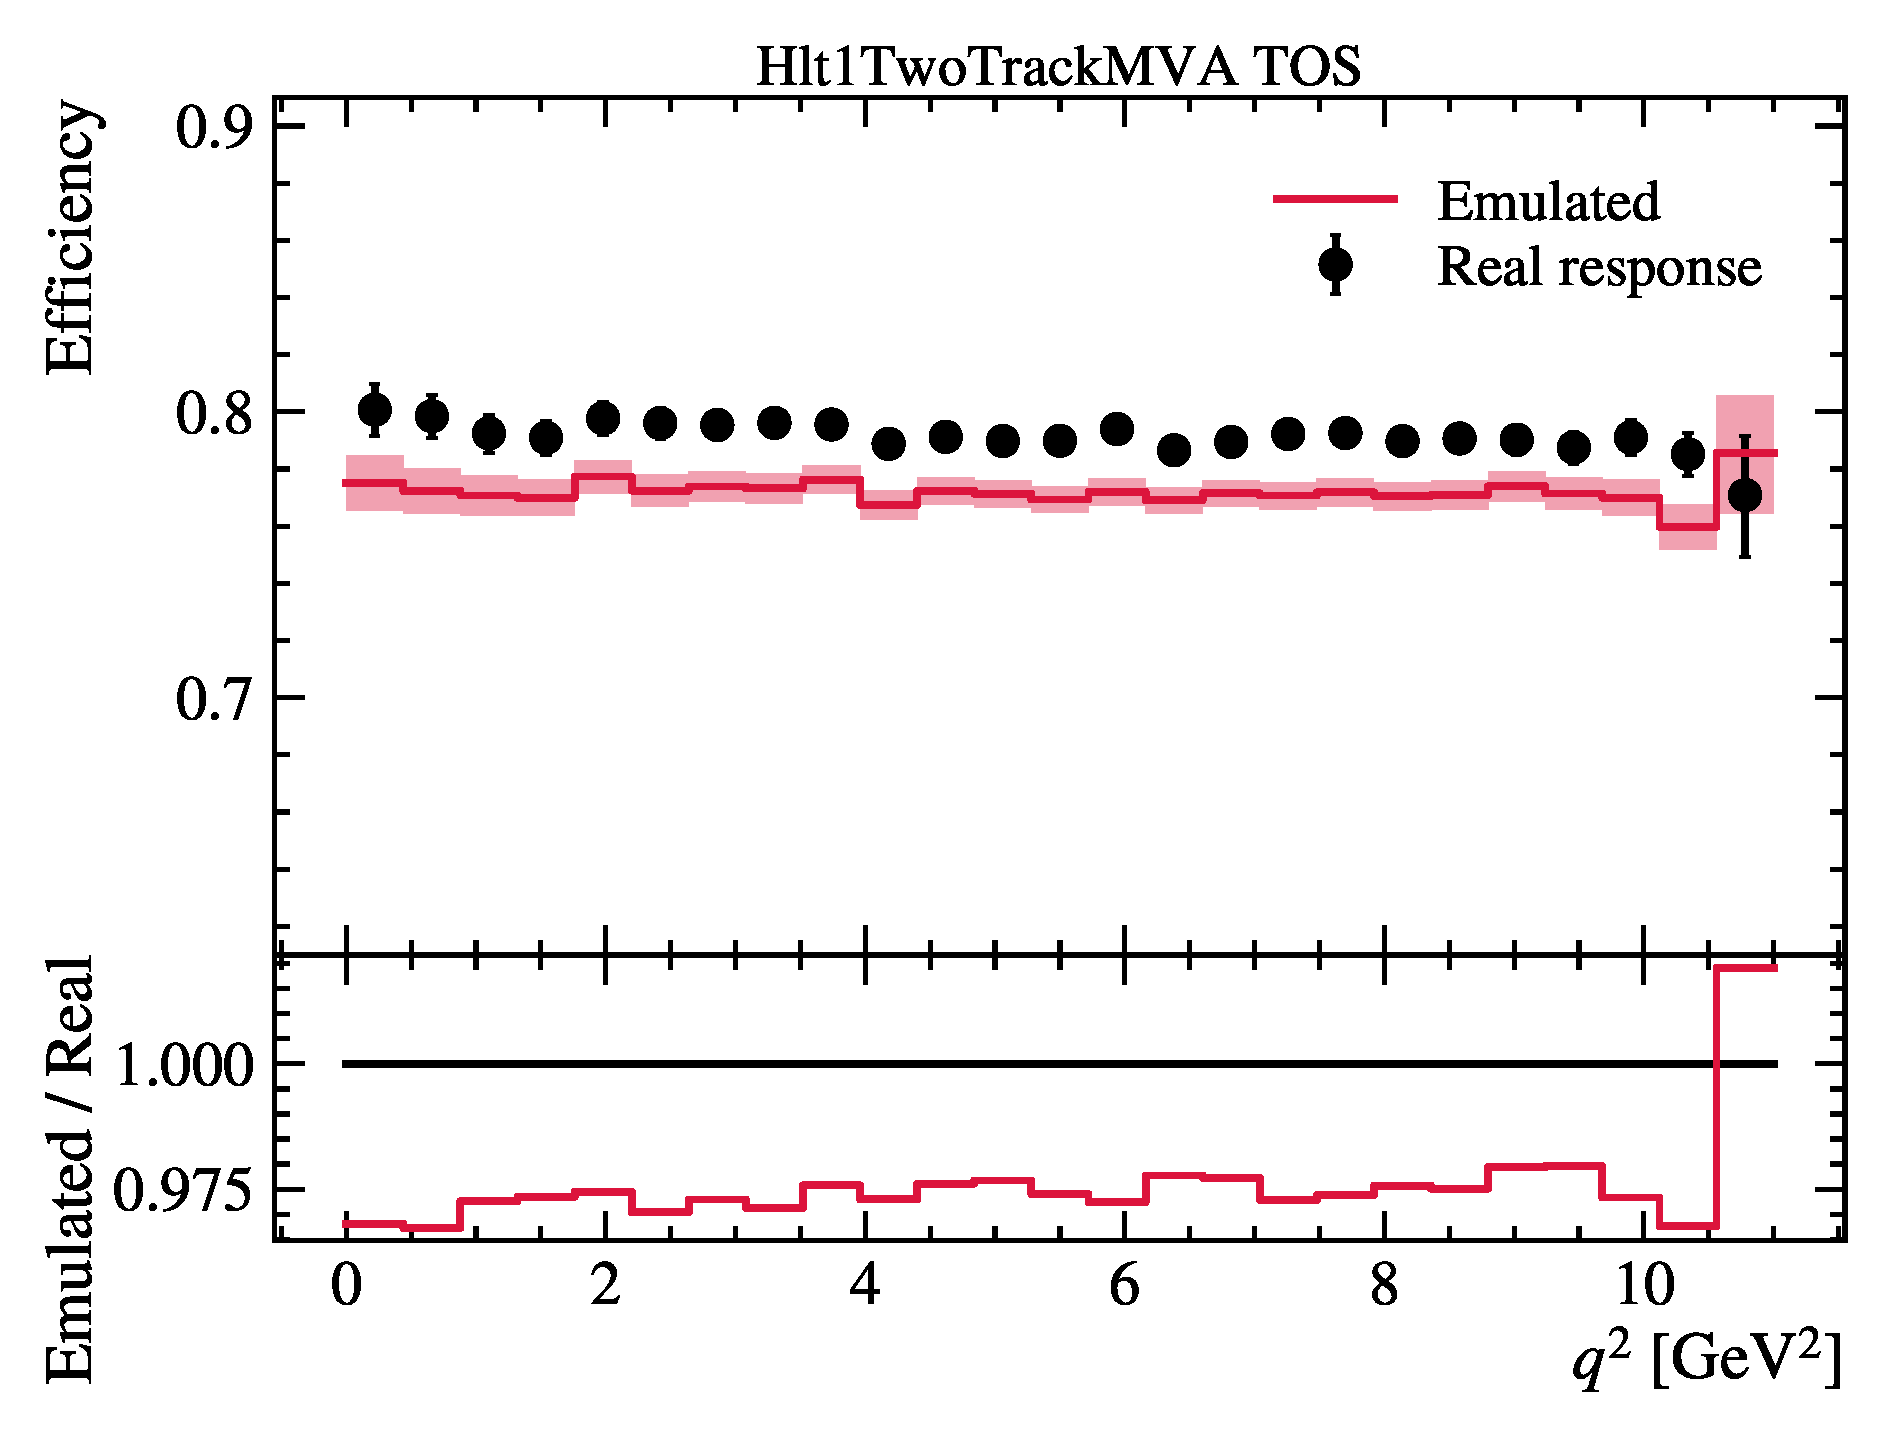
\includegraphics[width=0.32\textwidth]{
        ./figs-mc-emulation/emulate-hlt1/b0_Hlt1TwoTrackMVA_TOS_q2.pdf
    }

    \caption{
        Emualted HLT1 triggers in \Bz have similar level of agreement to real
        response compared to that of \Bp.
    }
    \label{fig:hlt1-twotrackmva-emu}
\end{figure}


\subsection{Emulation of Hlt2XcMuXForTauB2XcMu}

The selected \B is required to TOS on Hlt2XcMuXForTauB2XcMu. All selection
variables listed in \cref{tab:cut-hlt2} are available in the selection procedure
so these cuts are applied directly.


\section{Particle identification emulation}
\label{sec:emulation-for-to-mc:pid}

Tracker-Only MC has RICH and calorimeters, sub-detectors responsible for
particle identification (PID), set to passive material, thus no PID cut can be
applied directly on MC.
Therefore, PID cuts for MC are emulated as efficiencies (binned in some
variables, typically $p$, $\eta$, and nTracks) and applied as weights.

Most of PID efficiencies are obtained with \pidcalib, except for ghost and
$e$ \UBDT efficiencies. The ghost PID efficiencies are obtained from the bachelor
$\mu$ tracks truth-matched to ghost in
2016 inclusive $J/\psi K$ MC, % FIXME: MC IDs
and the $e$ \UBDT efficiency, a \emph{conditional efficiency}, is obtained from
$\mu$ track truth-matched to $e$ in 2016 $D^*\mu$ MC.

It is worth noting that \pidcalib does not populate under and overflow bins,
therefore an custom binning scheme, extended from the official scheme, is used
for \pidcalib efficiencies to ensure a wider coverage.

\techlink{appx:tech:obtain-pid-eff}

\chapter{Correction and validation of the MC simulation}
\label{ref:mc-cor}

This chapter describes corrections to MC,
mainly to correct the modelling of form factor and detector responses.
The MC correction procedure is the following:
%%%%
First, the outdated form factor modellings are updated and known
problematic responses, such as tracking efficiency and \B production kinematics,
are corrected.
This is termed as \emph{initial reweighting}, and is described in
\cref{sec:data-mc:init-rwt}.
%%%%
Then, a \emph{preliminary} fit is performed to build
\emph{post-fit cocktail},
with the building procedure outlined in \cref{sec:data-mc:postfit-cocktail}.
Finally, agreements between data and cocktail on additional kinematic
and geometric variables of the \B decay daughters are assessed,
and a multi-stage reweighting process is
performed to correct disagreements if necessary.
Outlined in \cref{sec:data-mc:final-rwt}, such procedure is called \emph{final
reweighting}.


\section{Initial reweighting}
\label{sec:data-mc:init-rwt}

\subsection{Form factor model}

The form factor model for a $B \rightarrow D \ell\neulb$ process \emph{defines}
the truth-level \qSq distribution (with angular variables integrated out) which
in turn affect the estimated \qSq which is a fit variable.
Therefore, it is important to use the state-of-art form factor models.
Naively this is hard, because the form model model is defined at MC generator
level, any change in form factor may require a regeneration of all MC samples.
In reality, however, for a given phase space point\footnote{
    The phase space is parameterized by \qSq and possibly angular variables,
    as defined in \cref{ref:theory:ff}.
}  \PSpt, the probability density that an event is generated \emph{at}
\PSpt is proportional to the differential decay rate evaluated at
\PSpt.
%%%%
For an event (or equivalently a given \PSpt point)
generated with an old form factor model,
its contribution (weight) in the new model is given by the ratio of differential
decay rates
\begin{equation}
    r = \left.
            \frac{d\Gamma_\text{new} / d\PSpt}{d\Gamma_\text{old} / d\PSpt}
        \right|_\text{eval at phase space point}
\end{equation}
So a change in form factor model is equivalently to a reweight, with weight given
by $r$.

\Hammer, the current state-of-art form factor reweighting program, is used
in this analysis to reweight
$B \rightarrow (\Dz| \Dstar| D^{**}) \lepton\neulb$ MC samples.
The details are given below.

\paragraph{\Dz}
The \Dz MC samples are generated with an up-to-date CLN form factor model.
Still, it is reweighted to a BGL model whose parameters are taken
from Table 4 in \cite{Bigi_2016} at $N = 2$, as these
parameters are obtained from a fit to lattice and experimental data.
The $N = 2$ is chosen because it is the only case where the correlation matrix
is reported.
\Cref{fig:ff-d0} shows the shift of true \qSq distributions due to form factor
reweighting for \Dz samples.
The changes are minimal because both models are up-to-date.

% Generated in /rdx-run2-analysis with:
%   make plot-all-ff-rwt
\begin{figure}[htb]
    \centering
    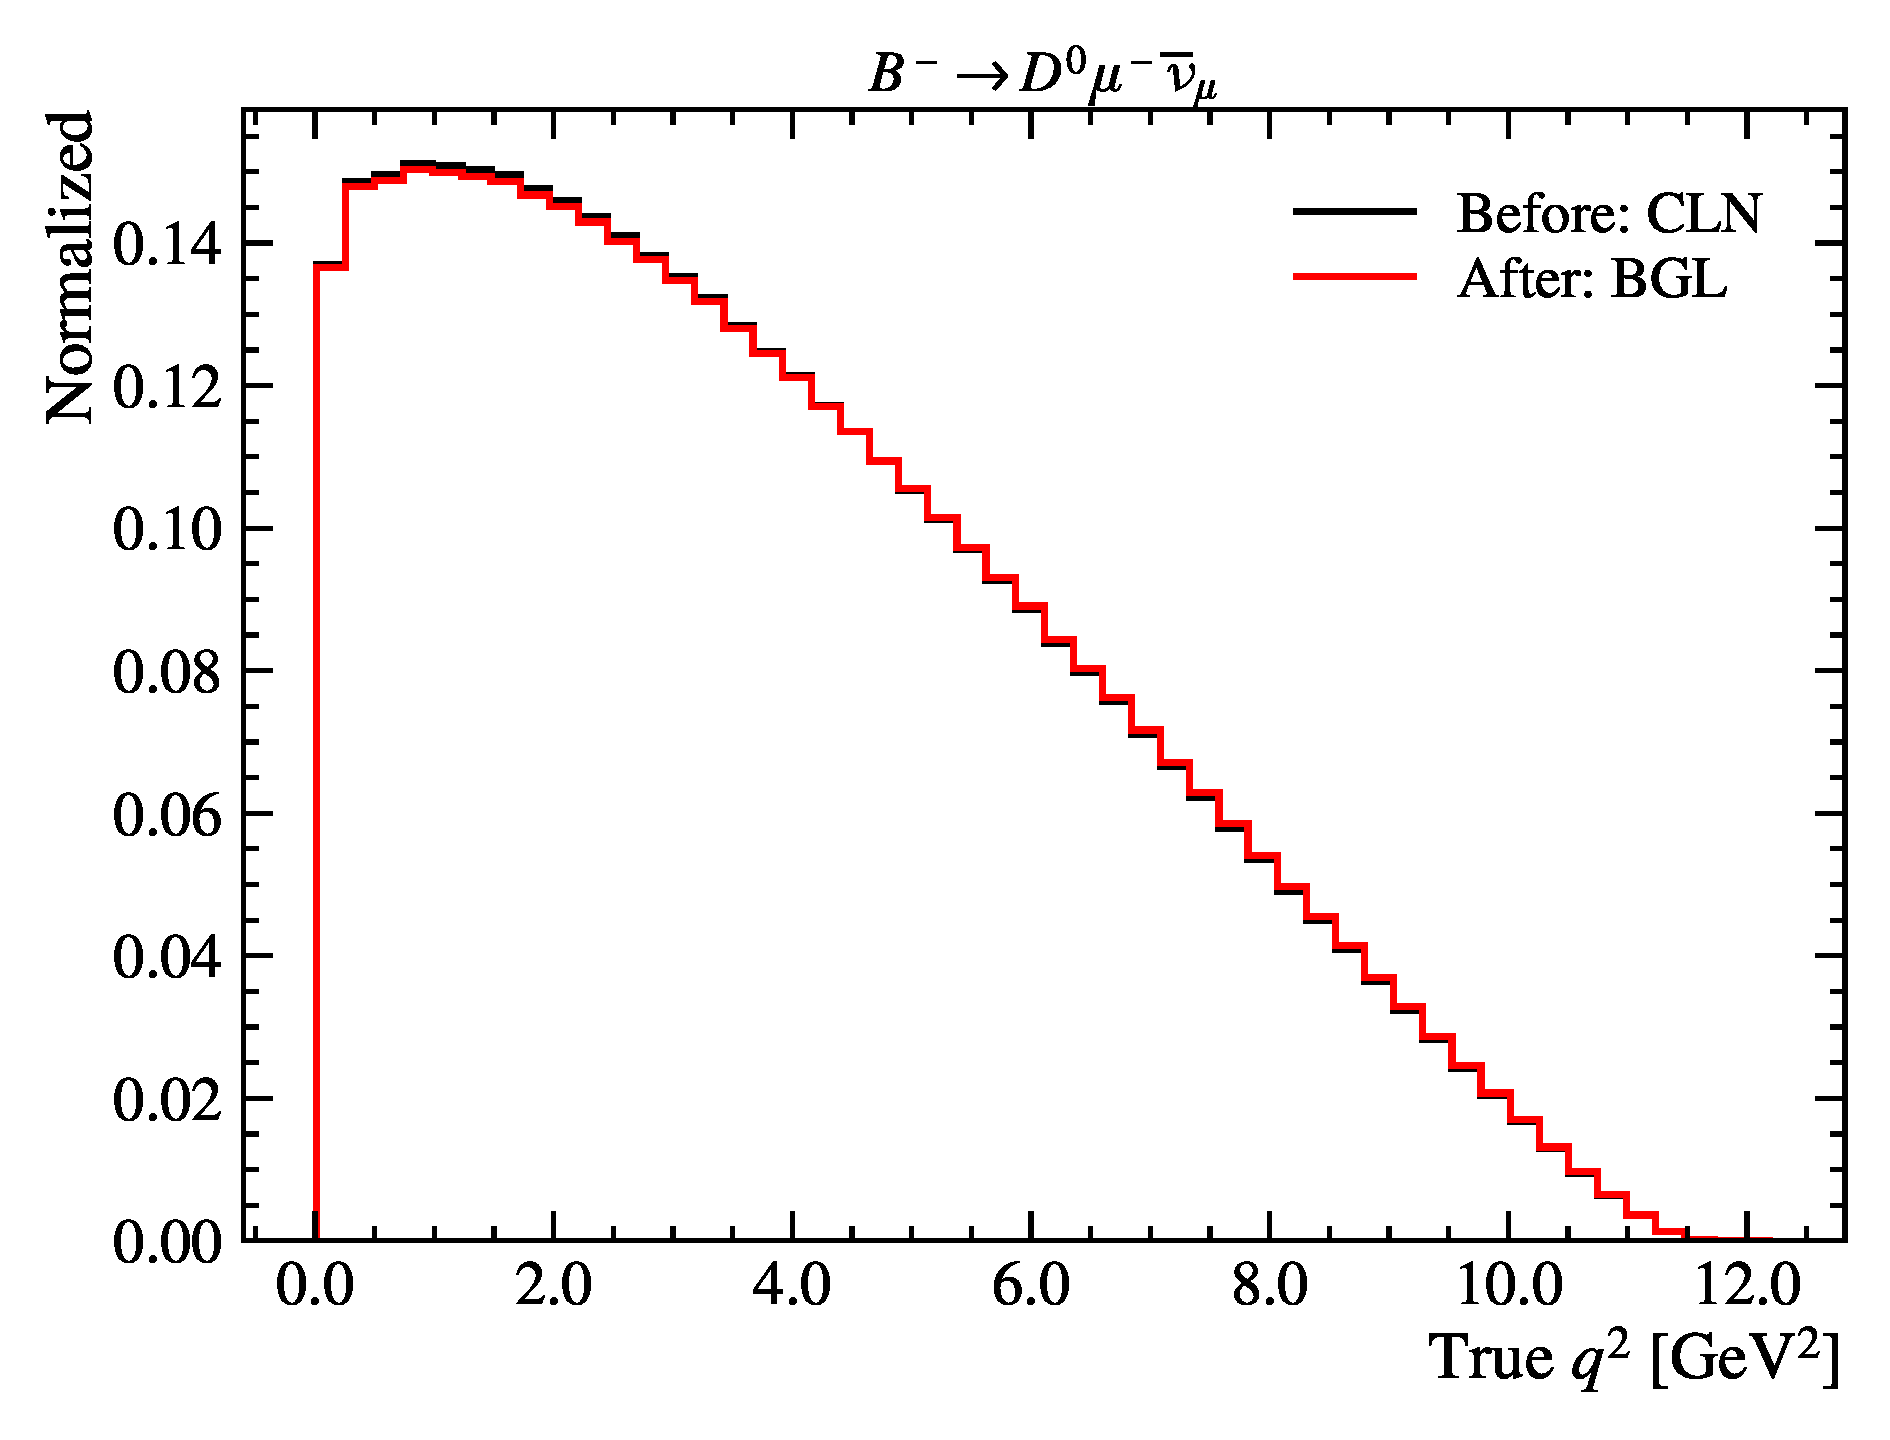
\includegraphics[width=0.45\textwidth]{
        ./figs-mc-correction/reweighting-form-factors/norm/D0Mu.pdf
    }
    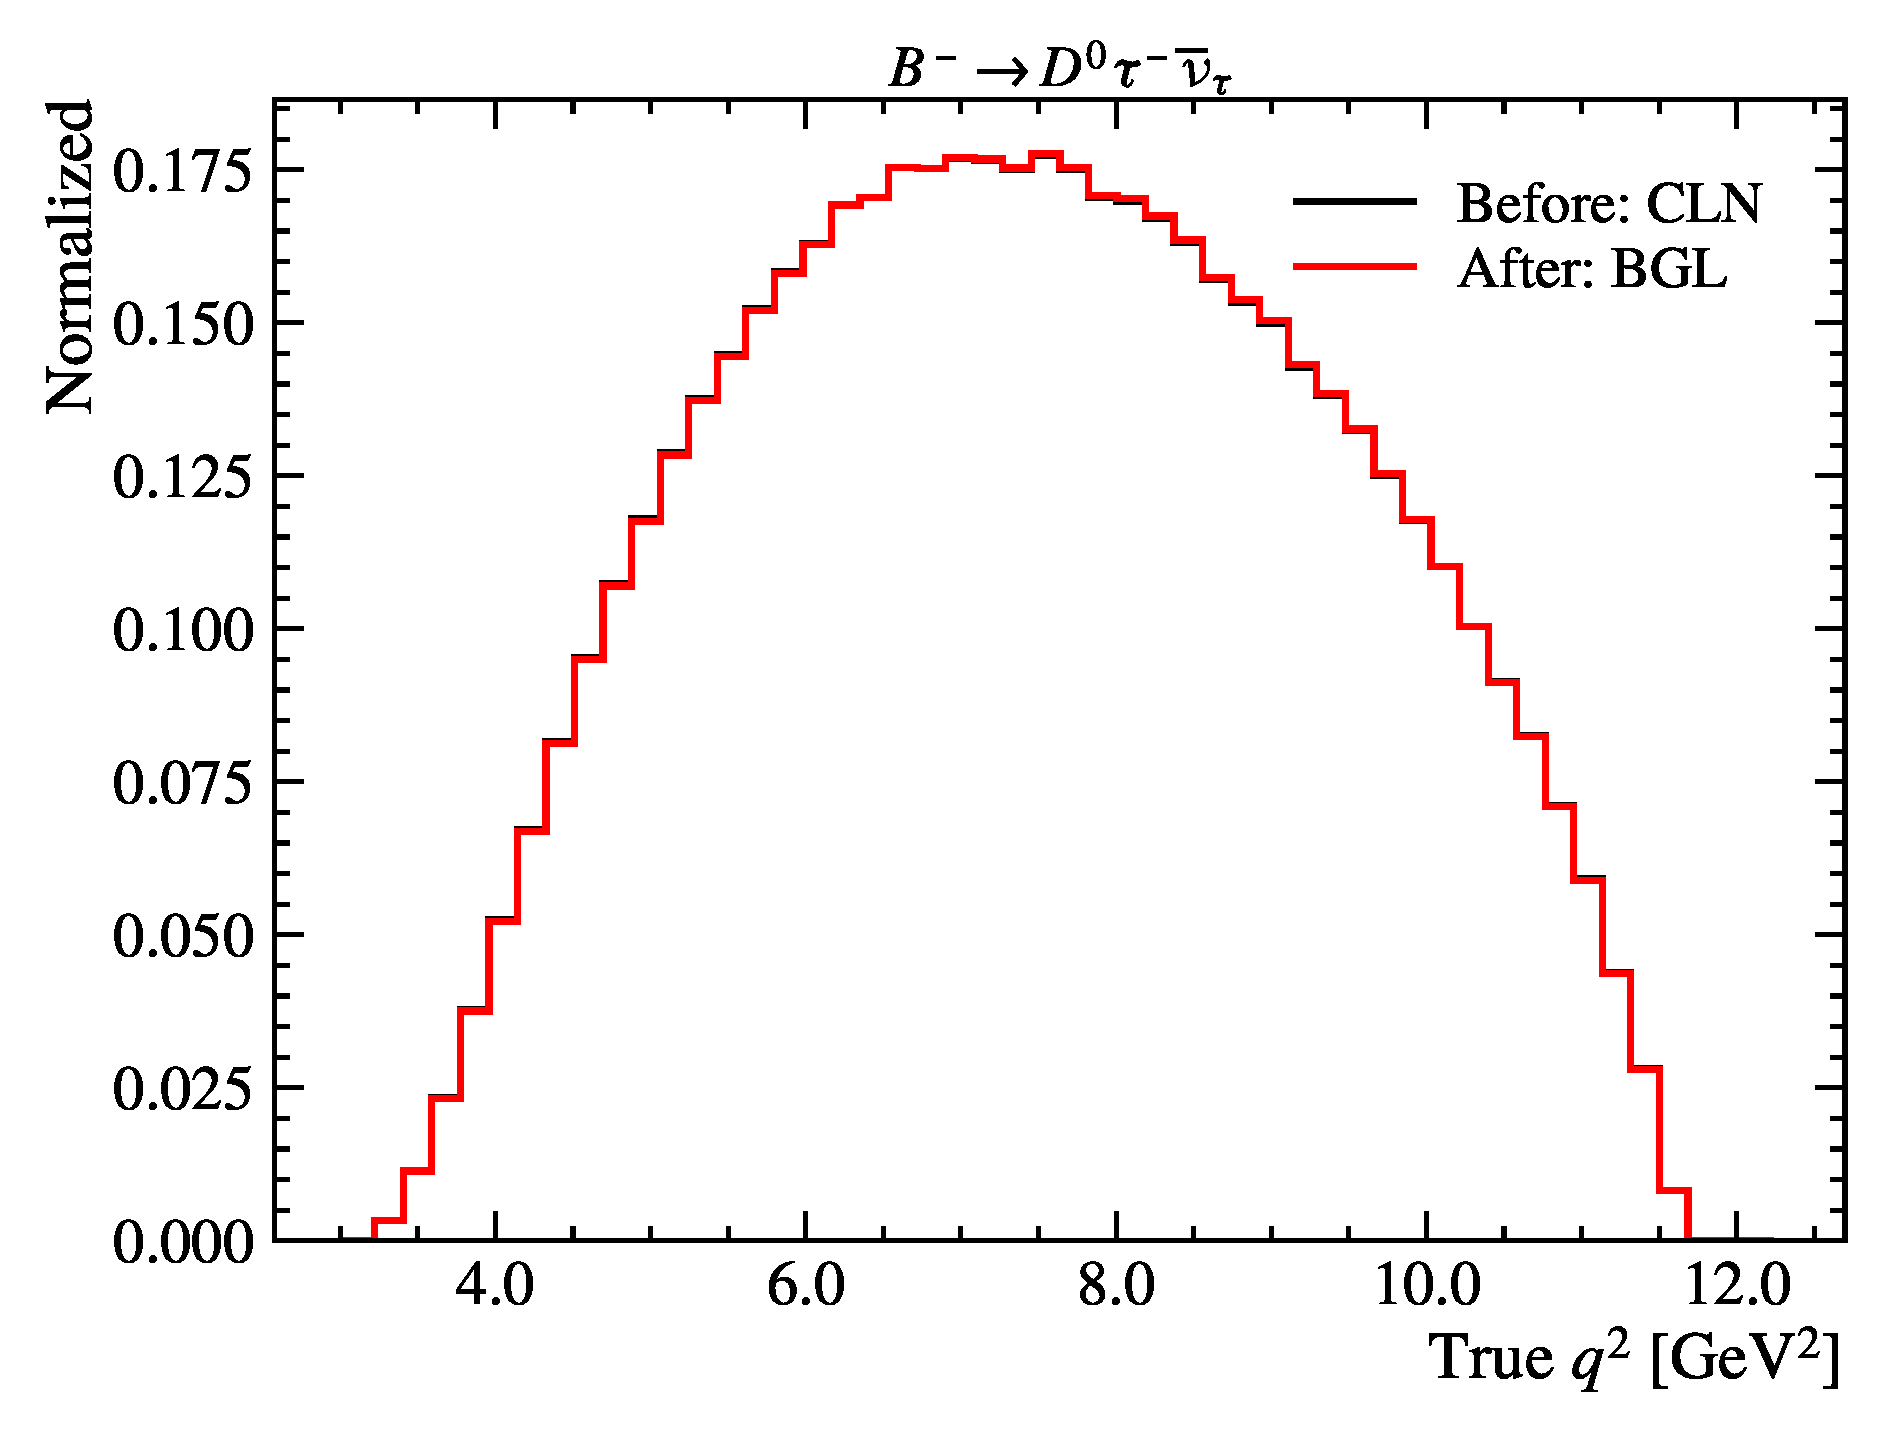
\includegraphics[width=0.45\textwidth]{
        ./figs-mc-correction/reweighting-form-factors/sig/D0Tau.pdf
    }
    \caption{
        Form factor reweight for $B \rightarrow \Dz \lepton\neulb$ MC samples.
    }
    \label{fig:ff-d0}
\end{figure}

\paragraph{\Dstar}
The \Dstar MC samples are reweighted from a CLN to a BGL model with parameters
taken from the right-most column of Table XII in the \textbf{v1} version of
\cite{Bazavov_2021},
the first work to calculate \Dstar form factors at non-zero recoil
based on lattice-QCD with constraints from external measurements.

The $c_3$ and $d_2$ parameters are not implemented in \Hammer (yet).
Given the large uncertainties on these sub-dominate parameters,
they are set to 0 with the corresponding entries in the covariance matrix
removed.

\begin{figure}[htb]
    \centering
    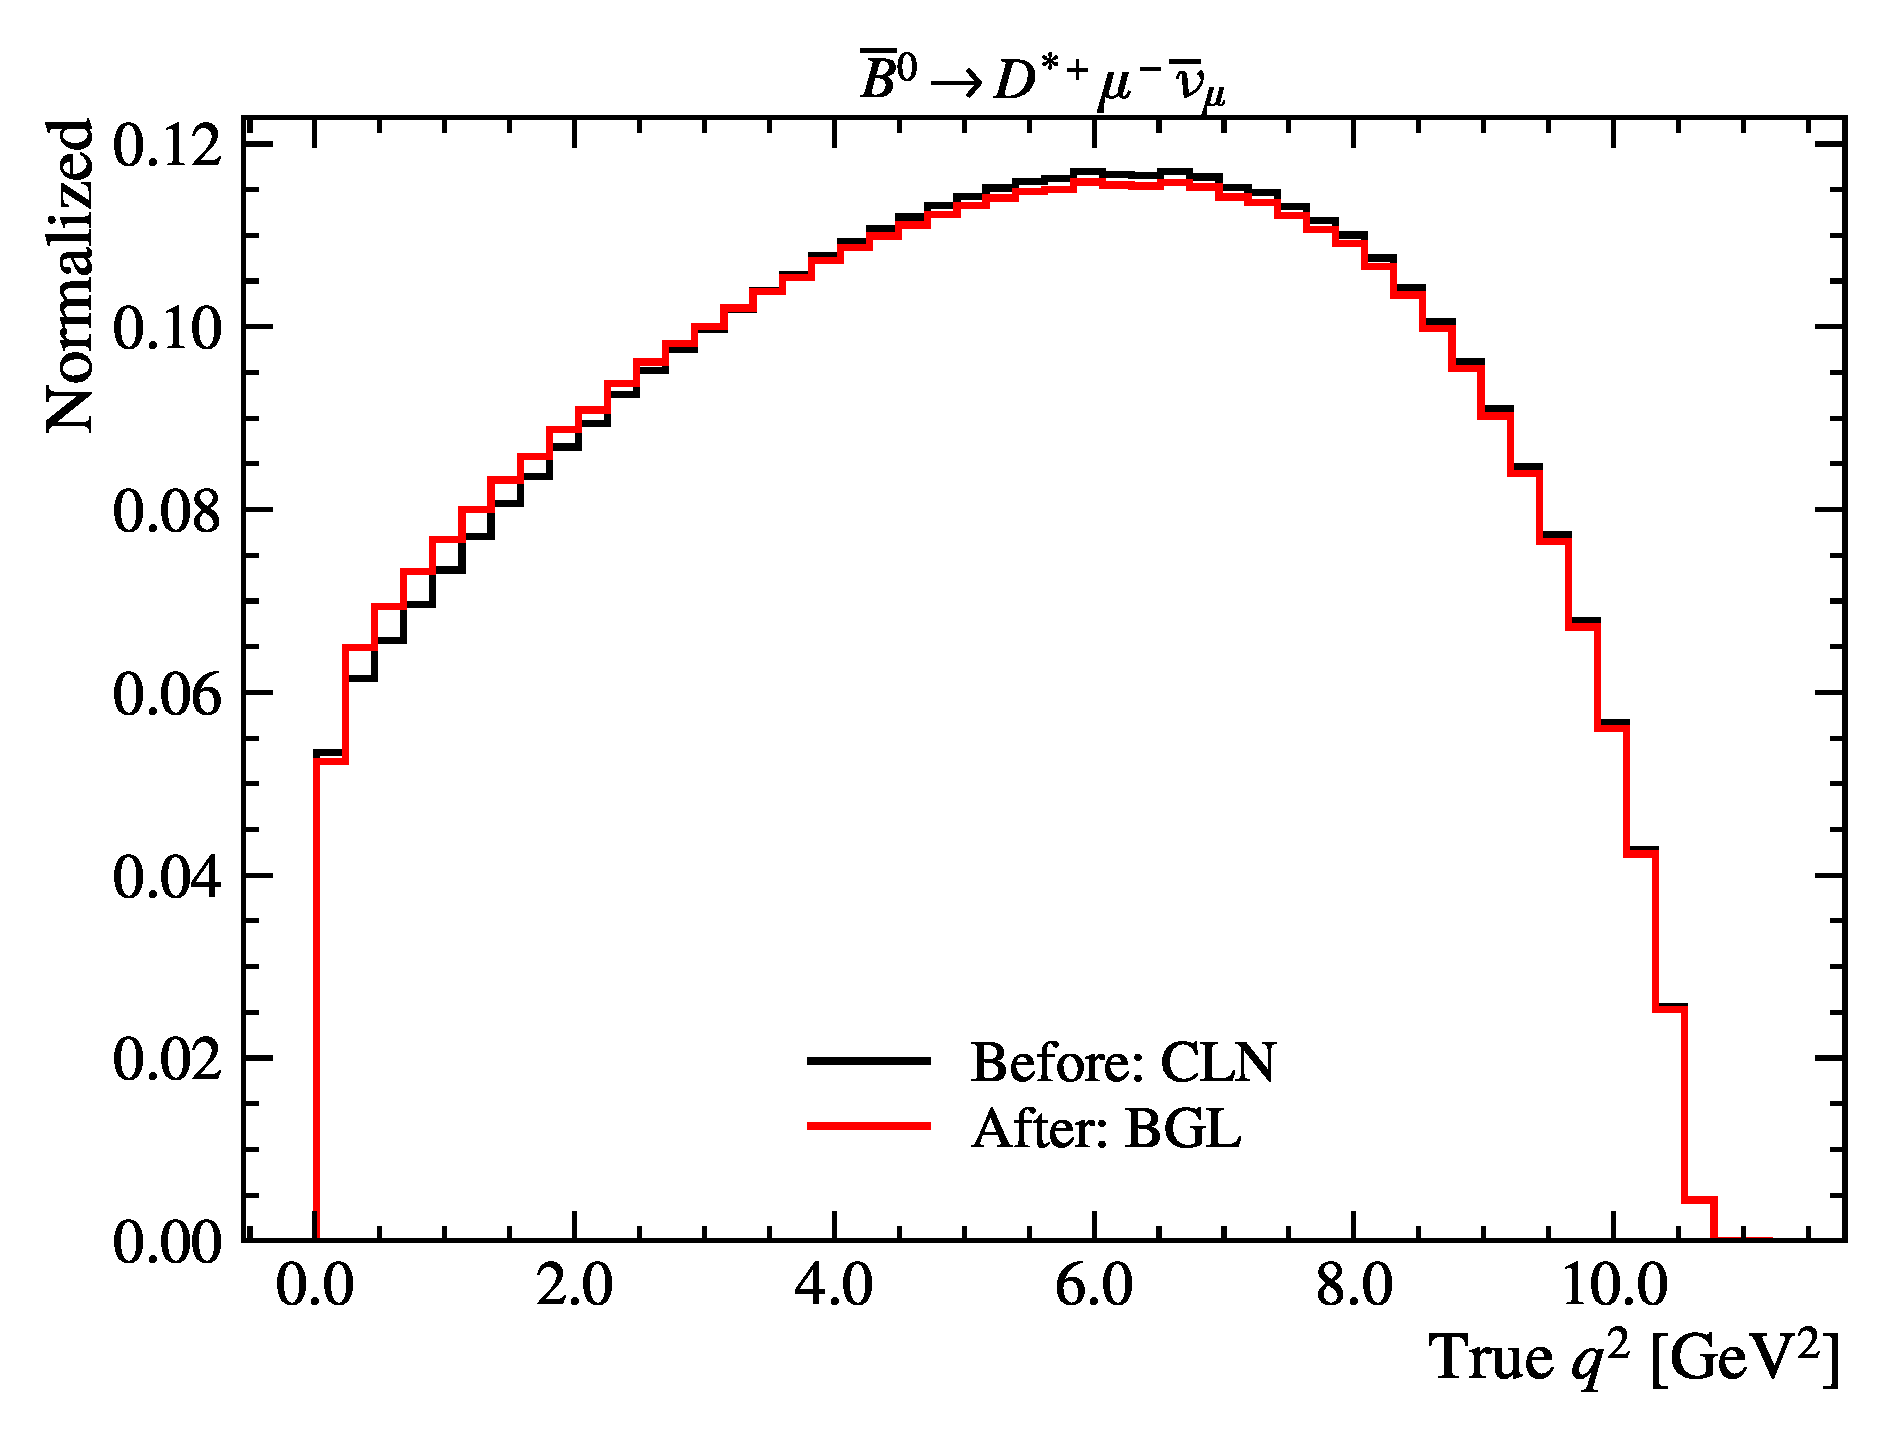
\includegraphics[width=0.45\textwidth]{
        ./figs-mc-correction/reweighting-form-factors/norm/DstMu.pdf
    }
    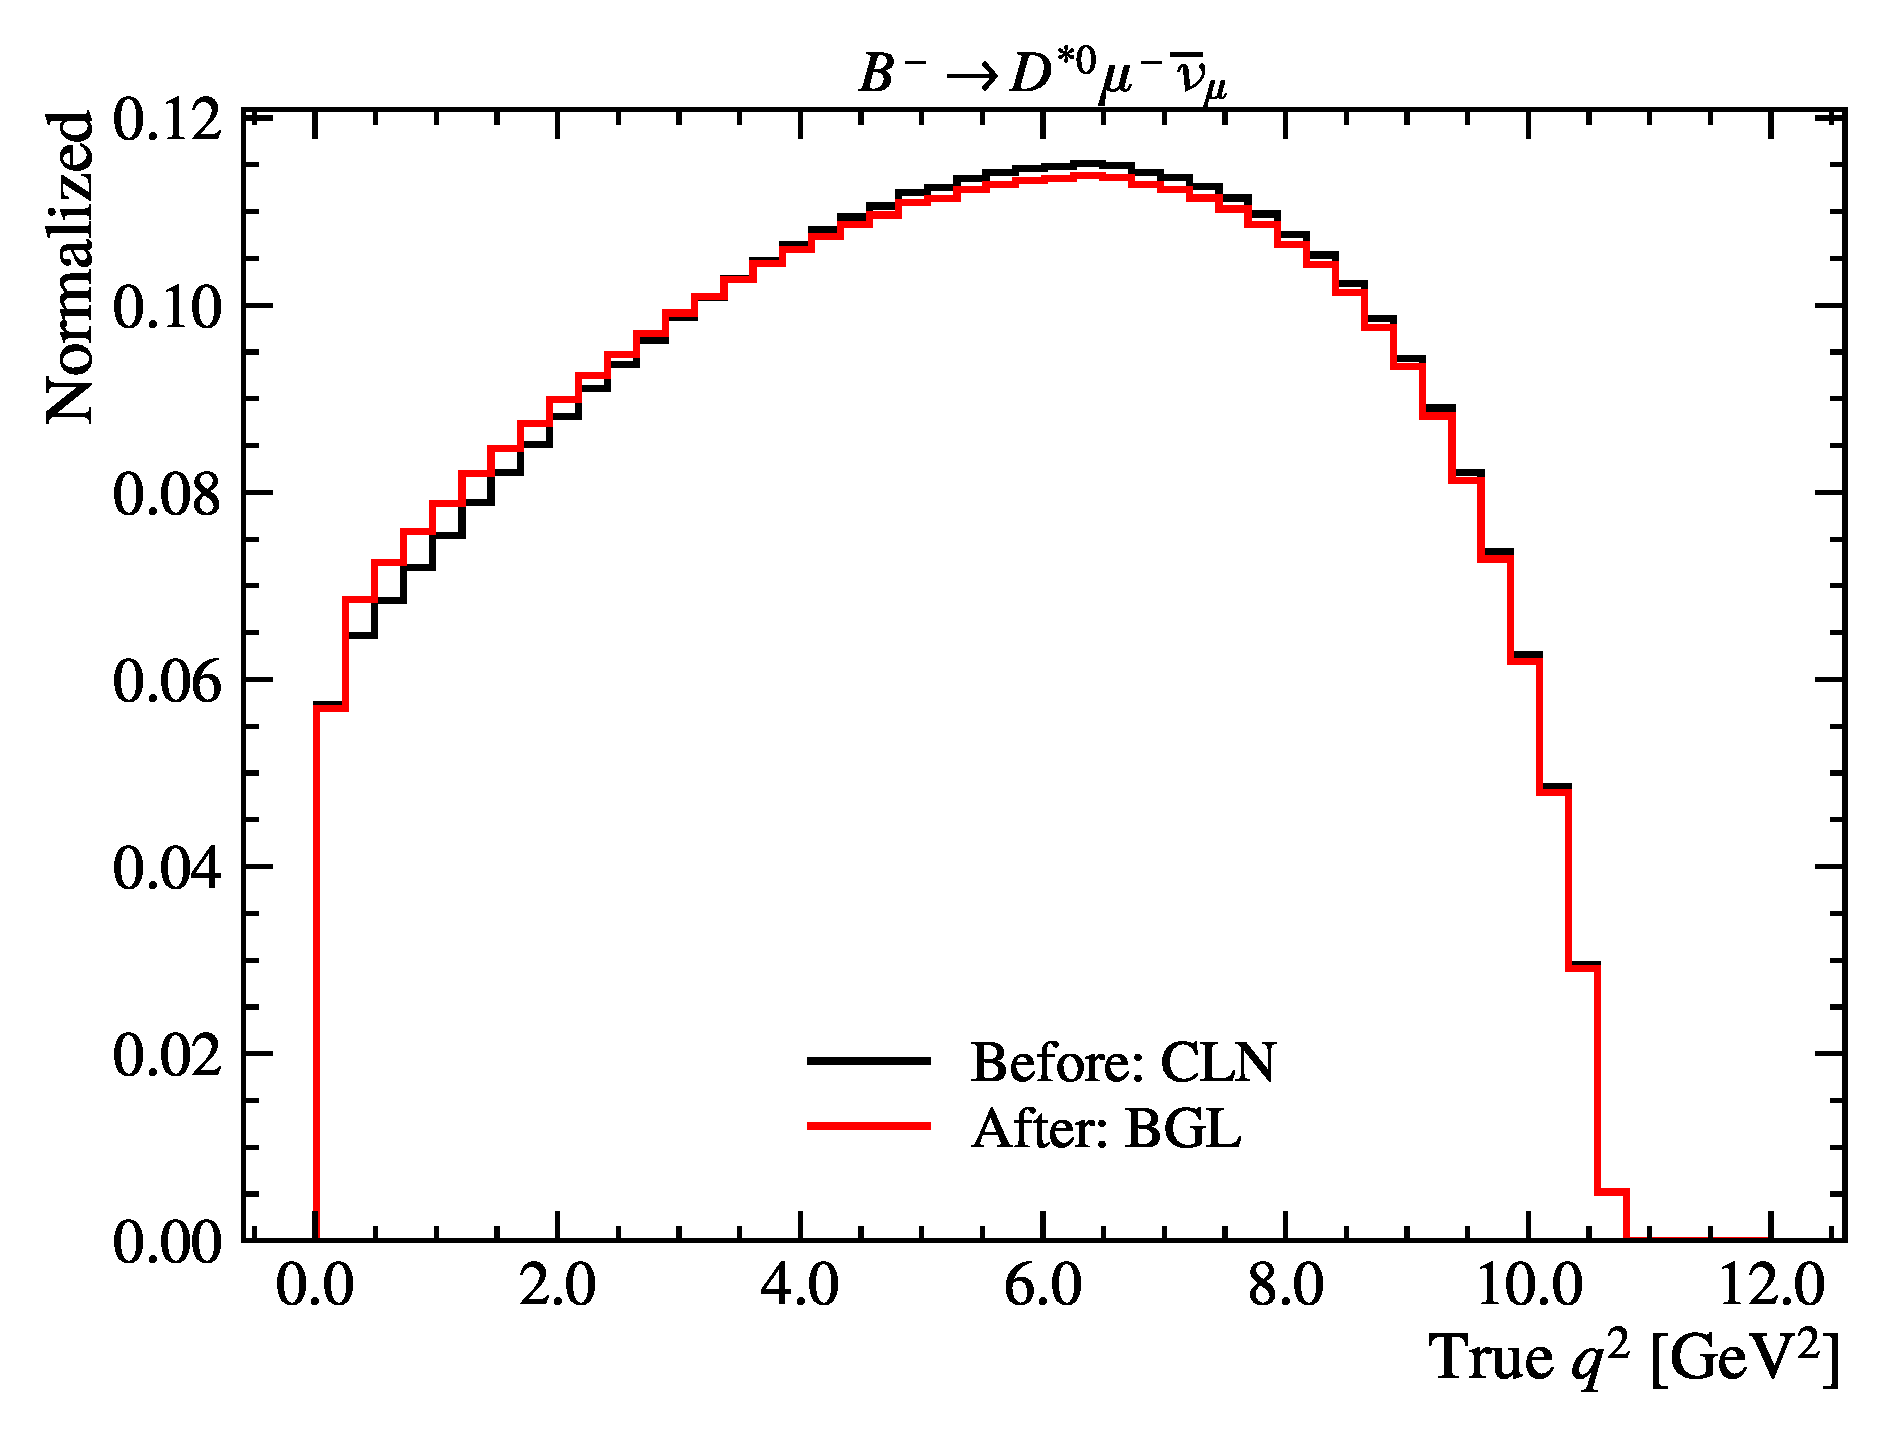
\includegraphics[width=0.45\textwidth]{
        ./figs-mc-correction/reweighting-form-factors/norm/Dst0Mu.pdf
    }

    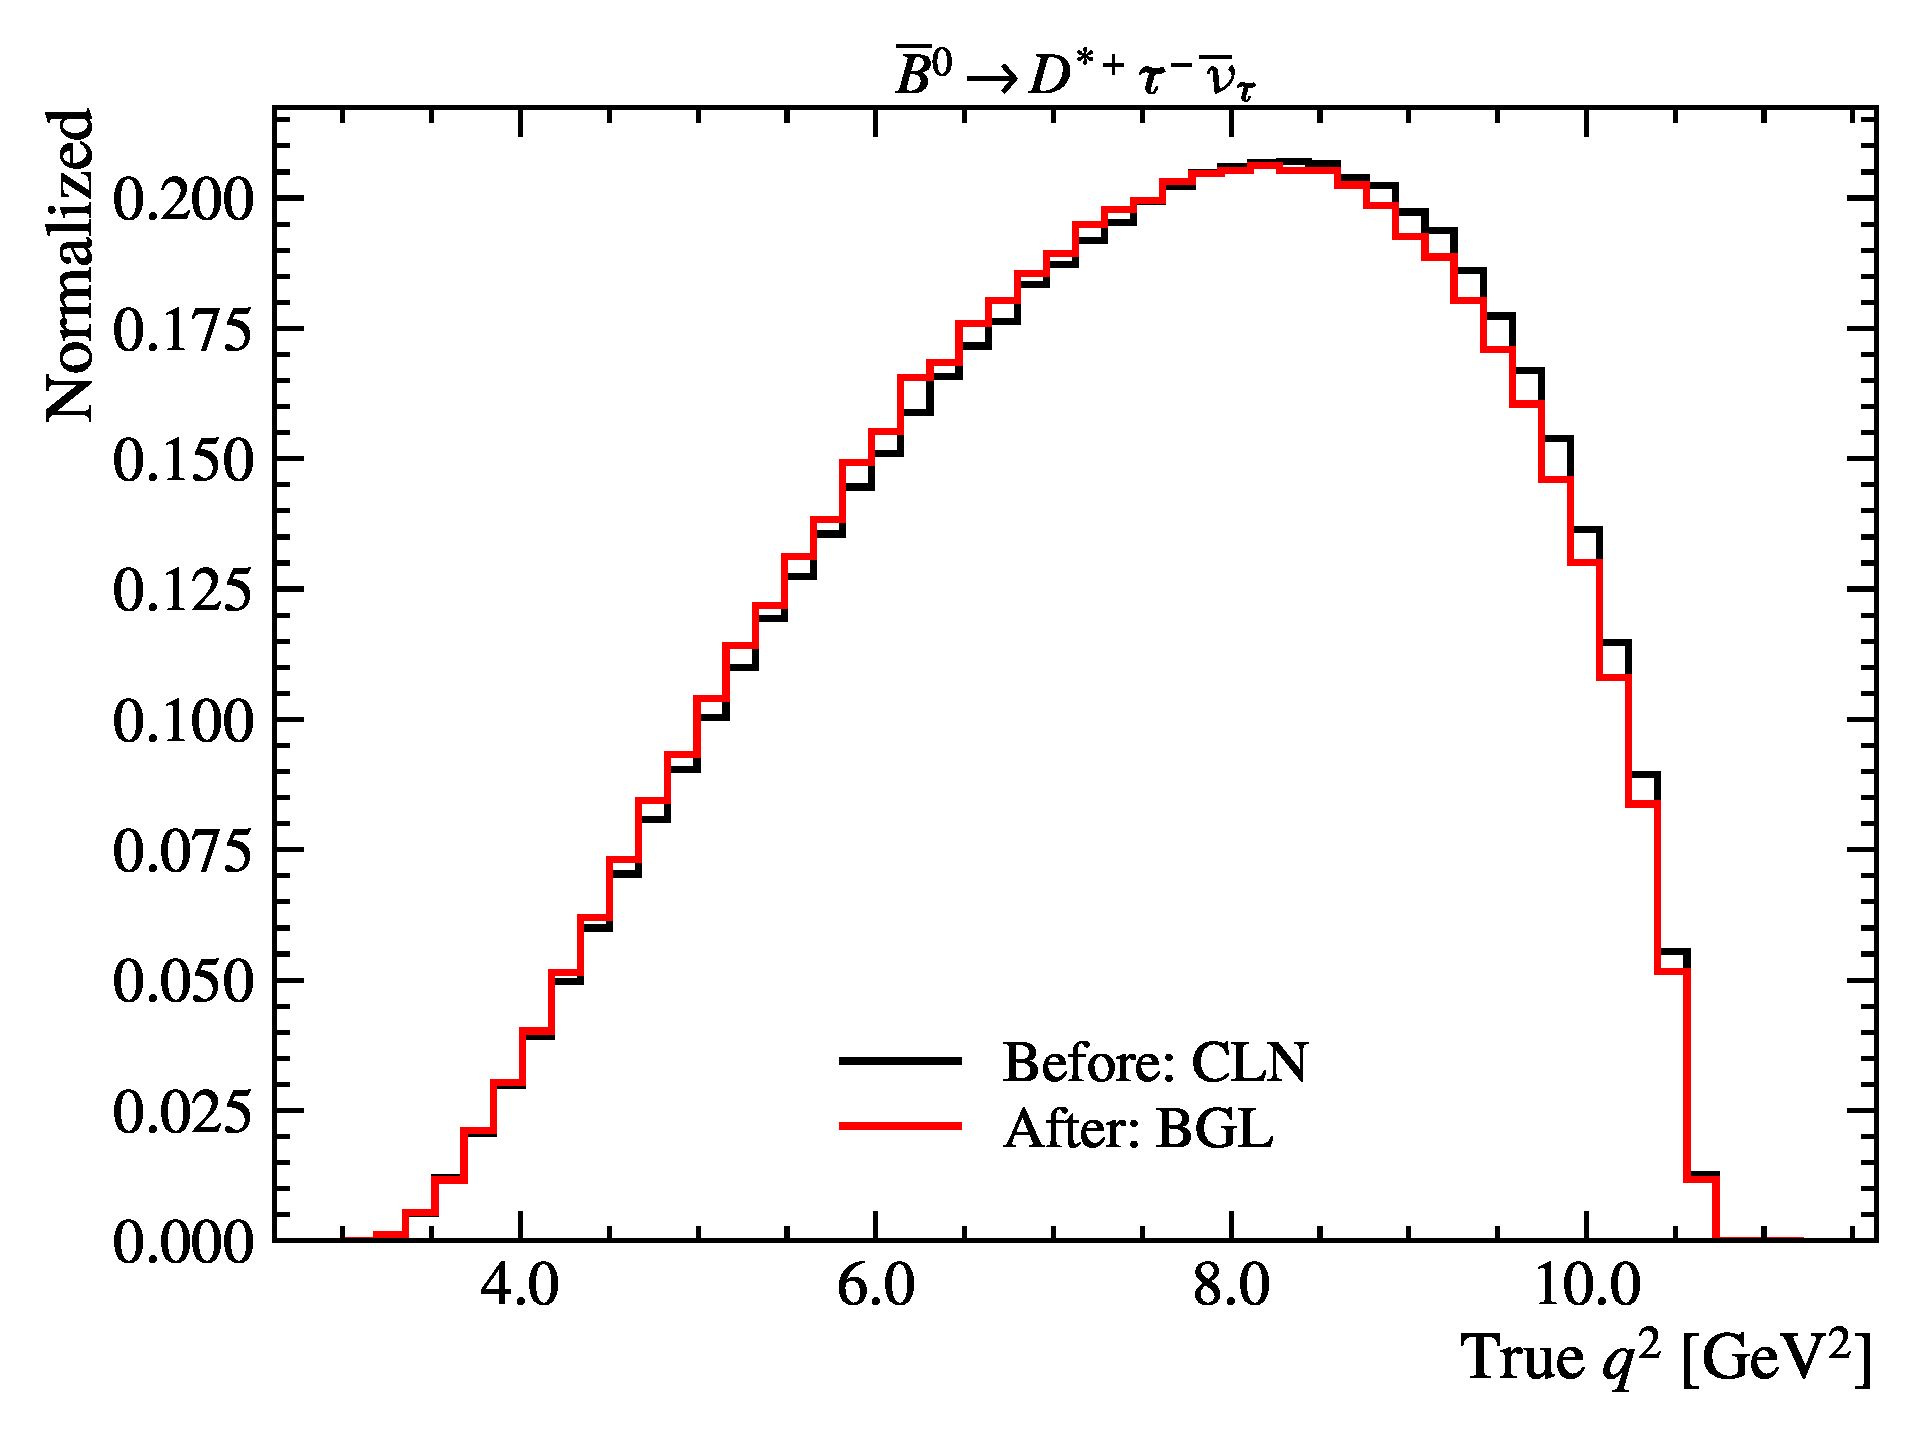
\includegraphics[width=0.45\textwidth]{
        ./figs-mc-correction/reweighting-form-factors/sig/DstTau.pdf
    }
    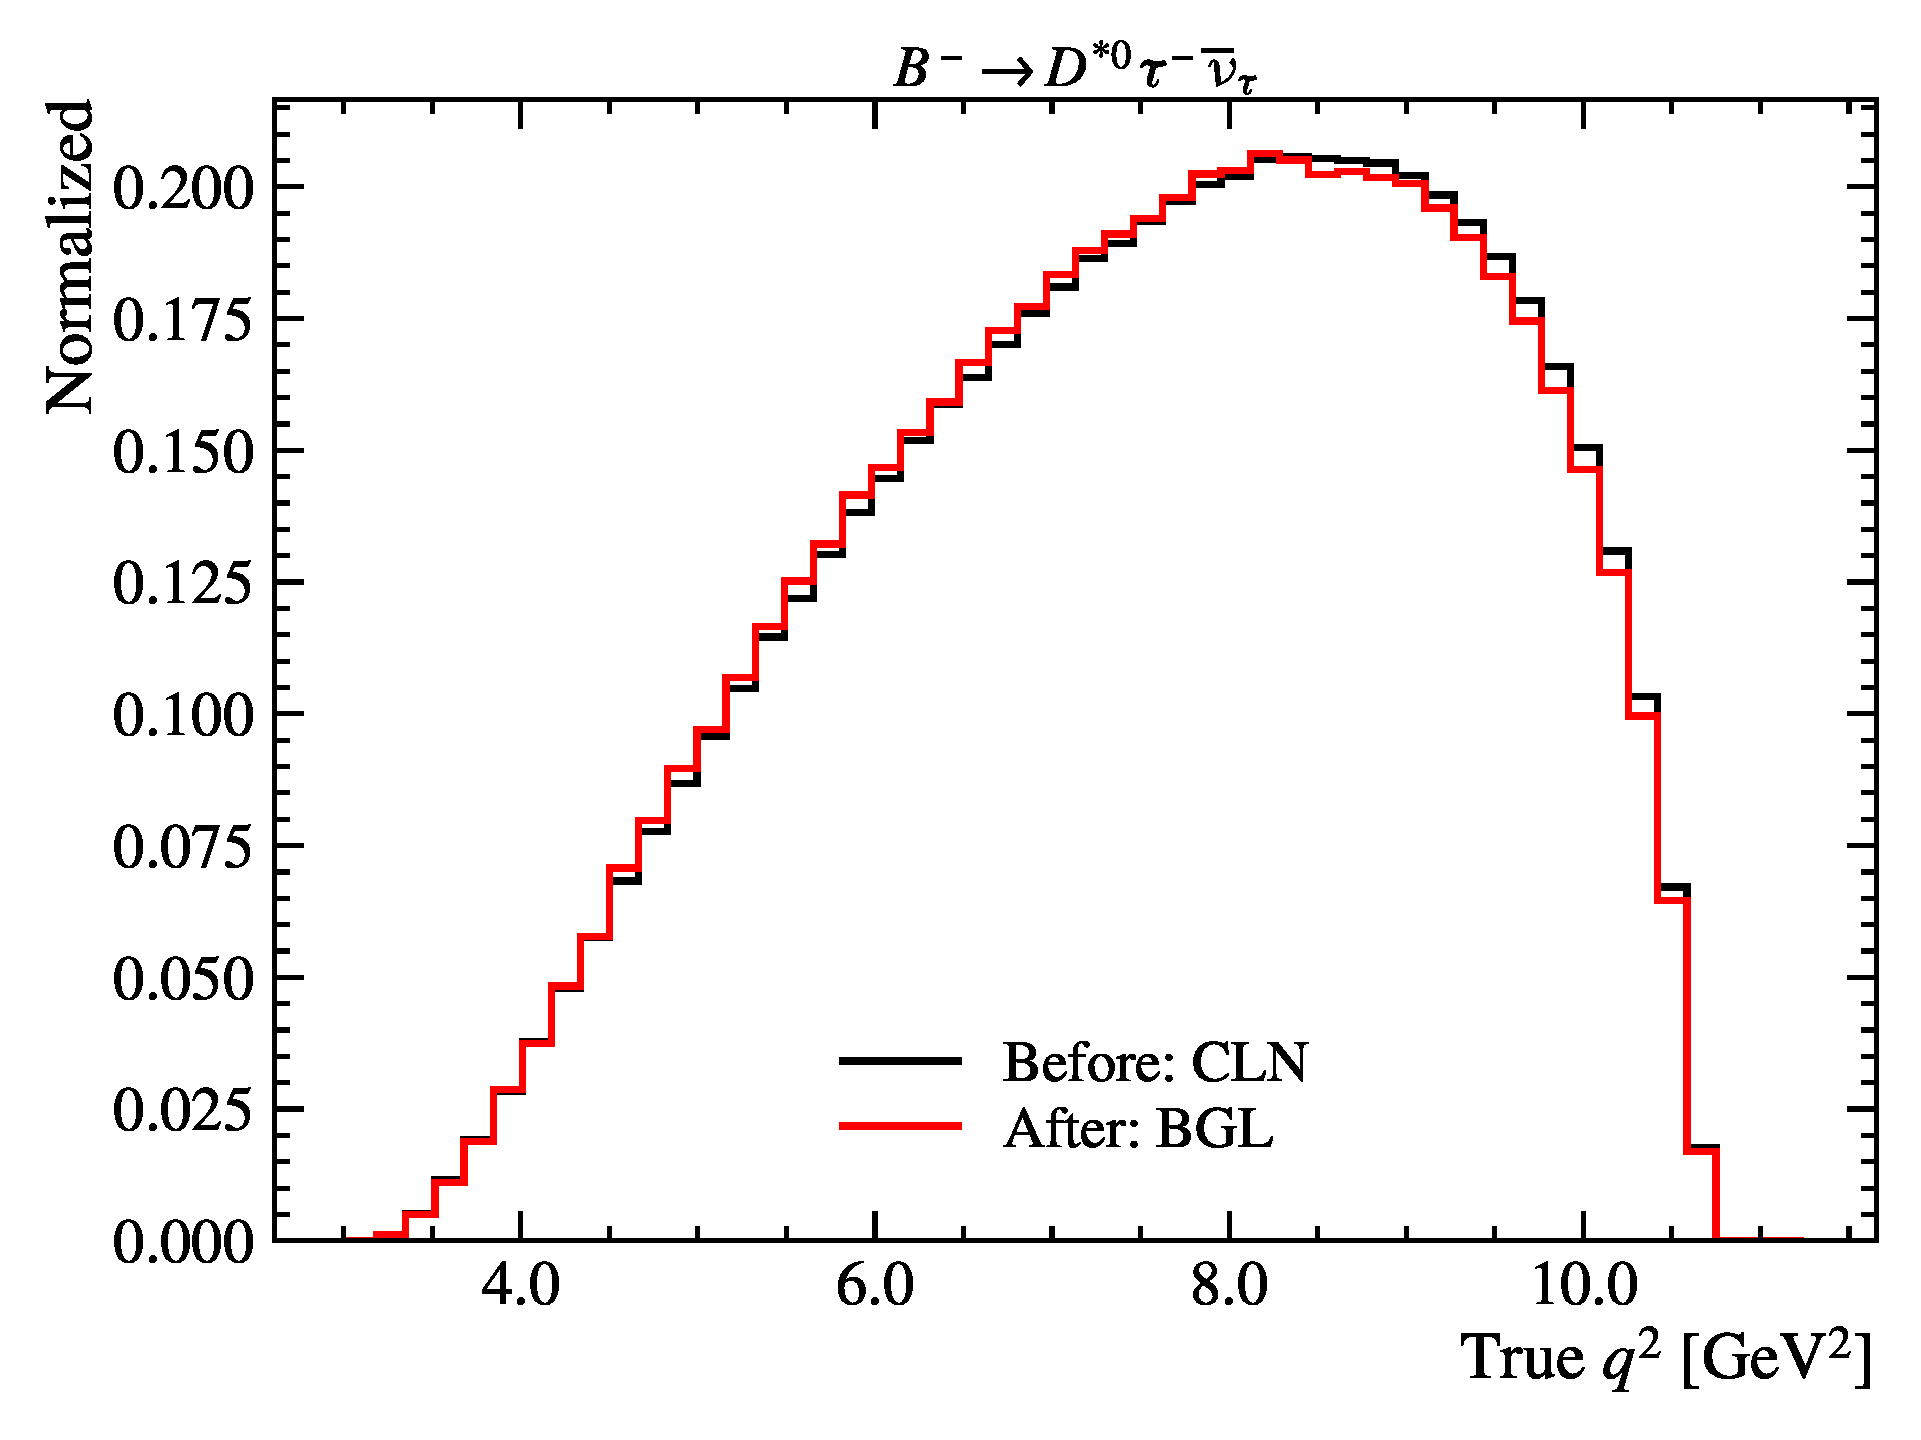
\includegraphics[width=0.45\textwidth]{
        ./figs-mc-correction/reweighting-form-factors/sig/Dst0Tau.pdf
    }
    \caption{
        Form factor reweight for $B \rightarrow \D^* \lepton\neulb$ MC samples.
    }
    \label{fig:ff-d0}
\end{figure}

\paragraph{$D^{**}$}
The four $1P$ $D^{**}$ states ($D^*_0$, $D_1$, $D'_1$, $D^*_2$) with decay mode
$B \rightarrow D^{**}\lepton\neulb$,
generated with ISGW2 form factor model,
are reweighted to BLR model.

\begin{figure}[ht]
    \centering
    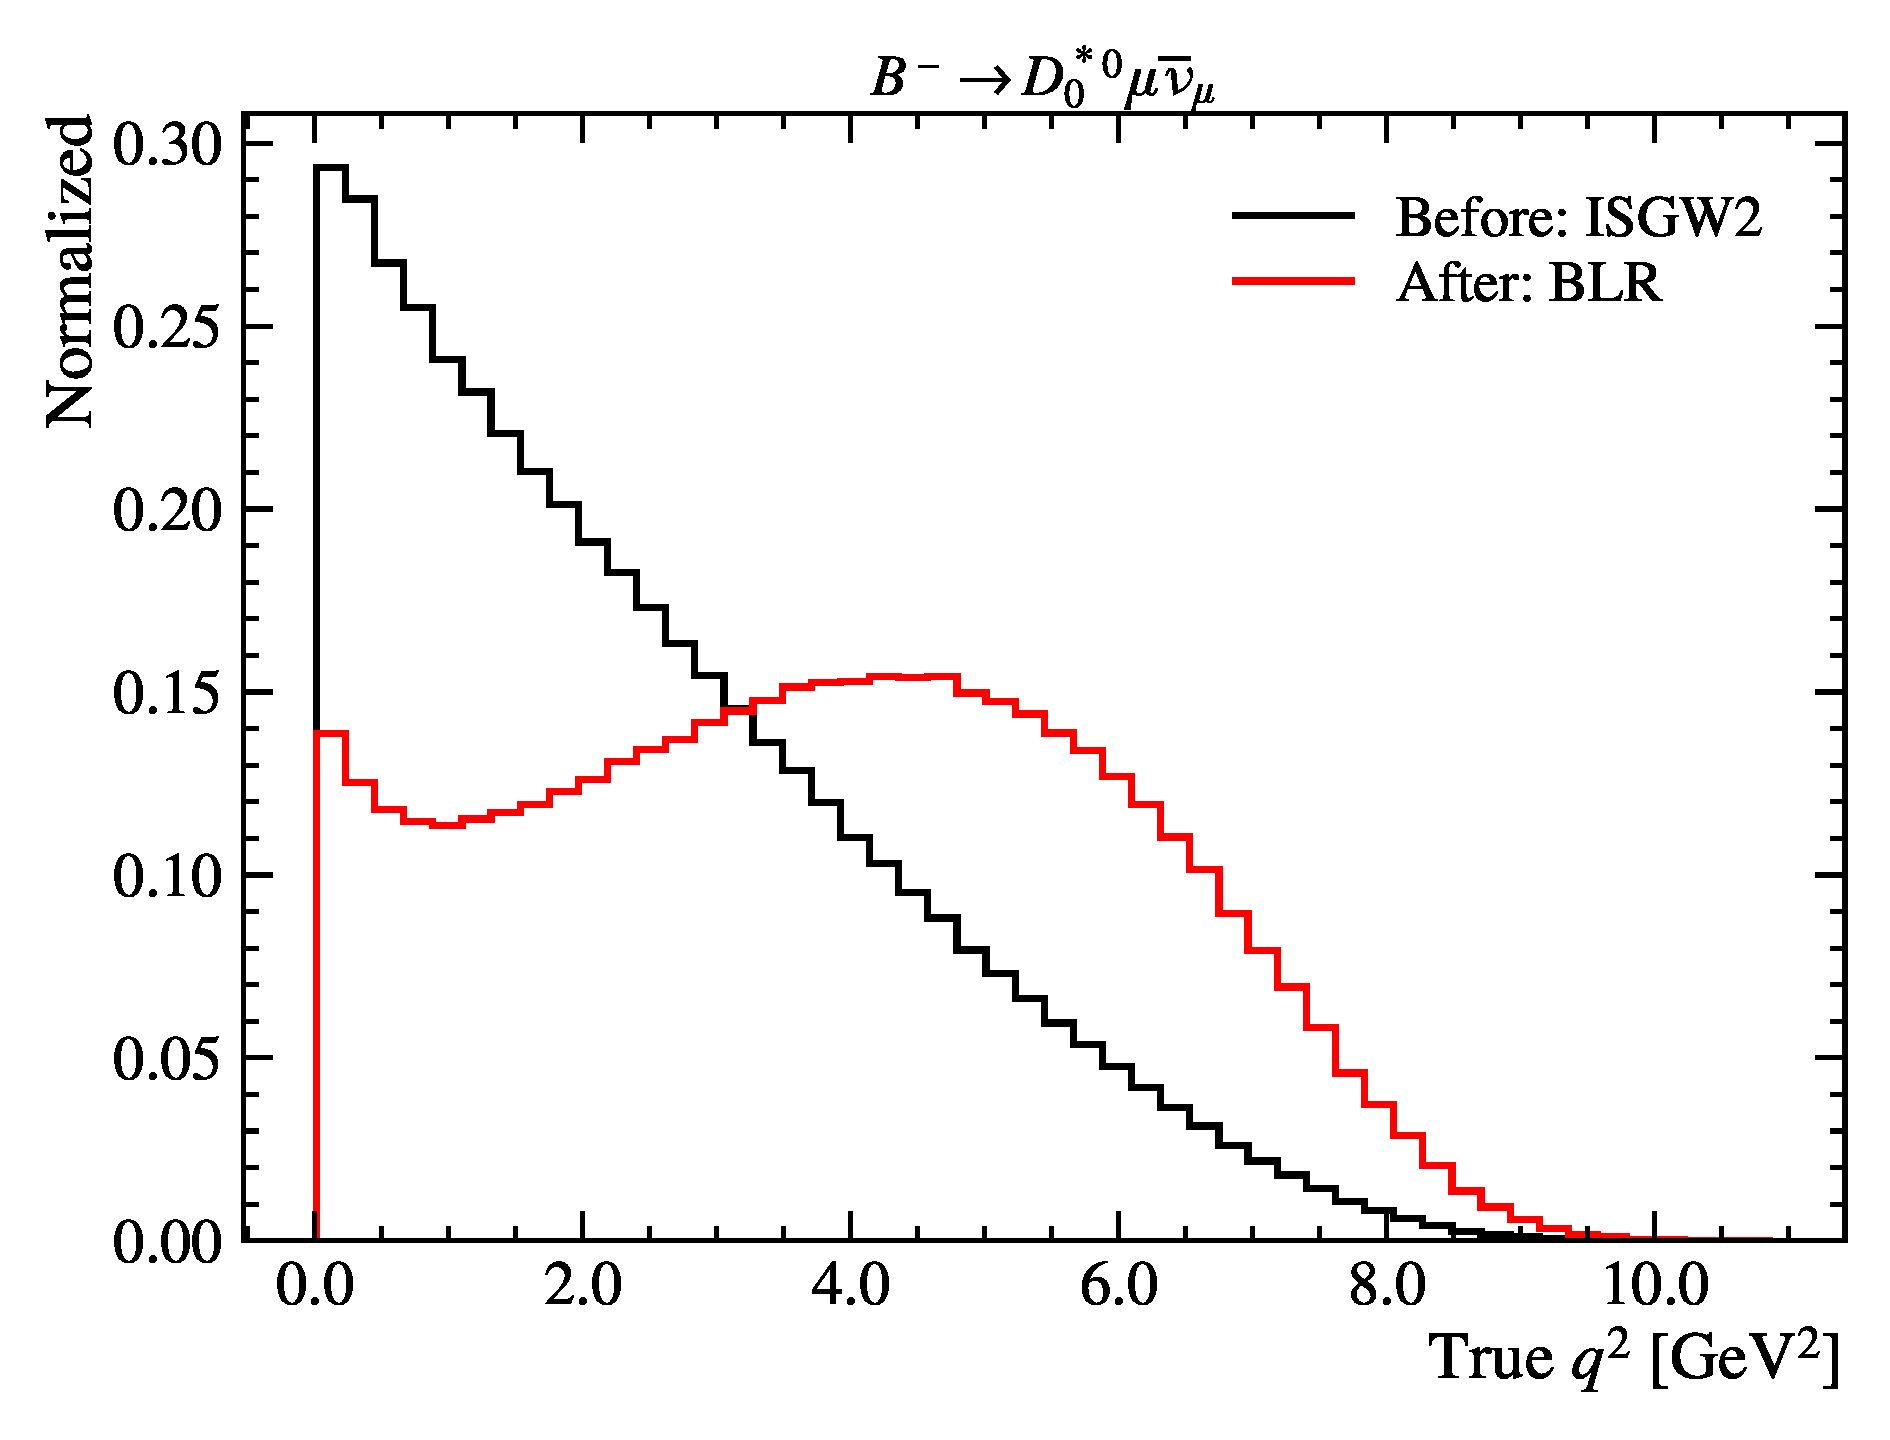
\includegraphics[width=0.24\textwidth]{
        ./figs-mc-correction/reweighting-form-factors/DststMu/D0stst0Mu.pdf
    }
    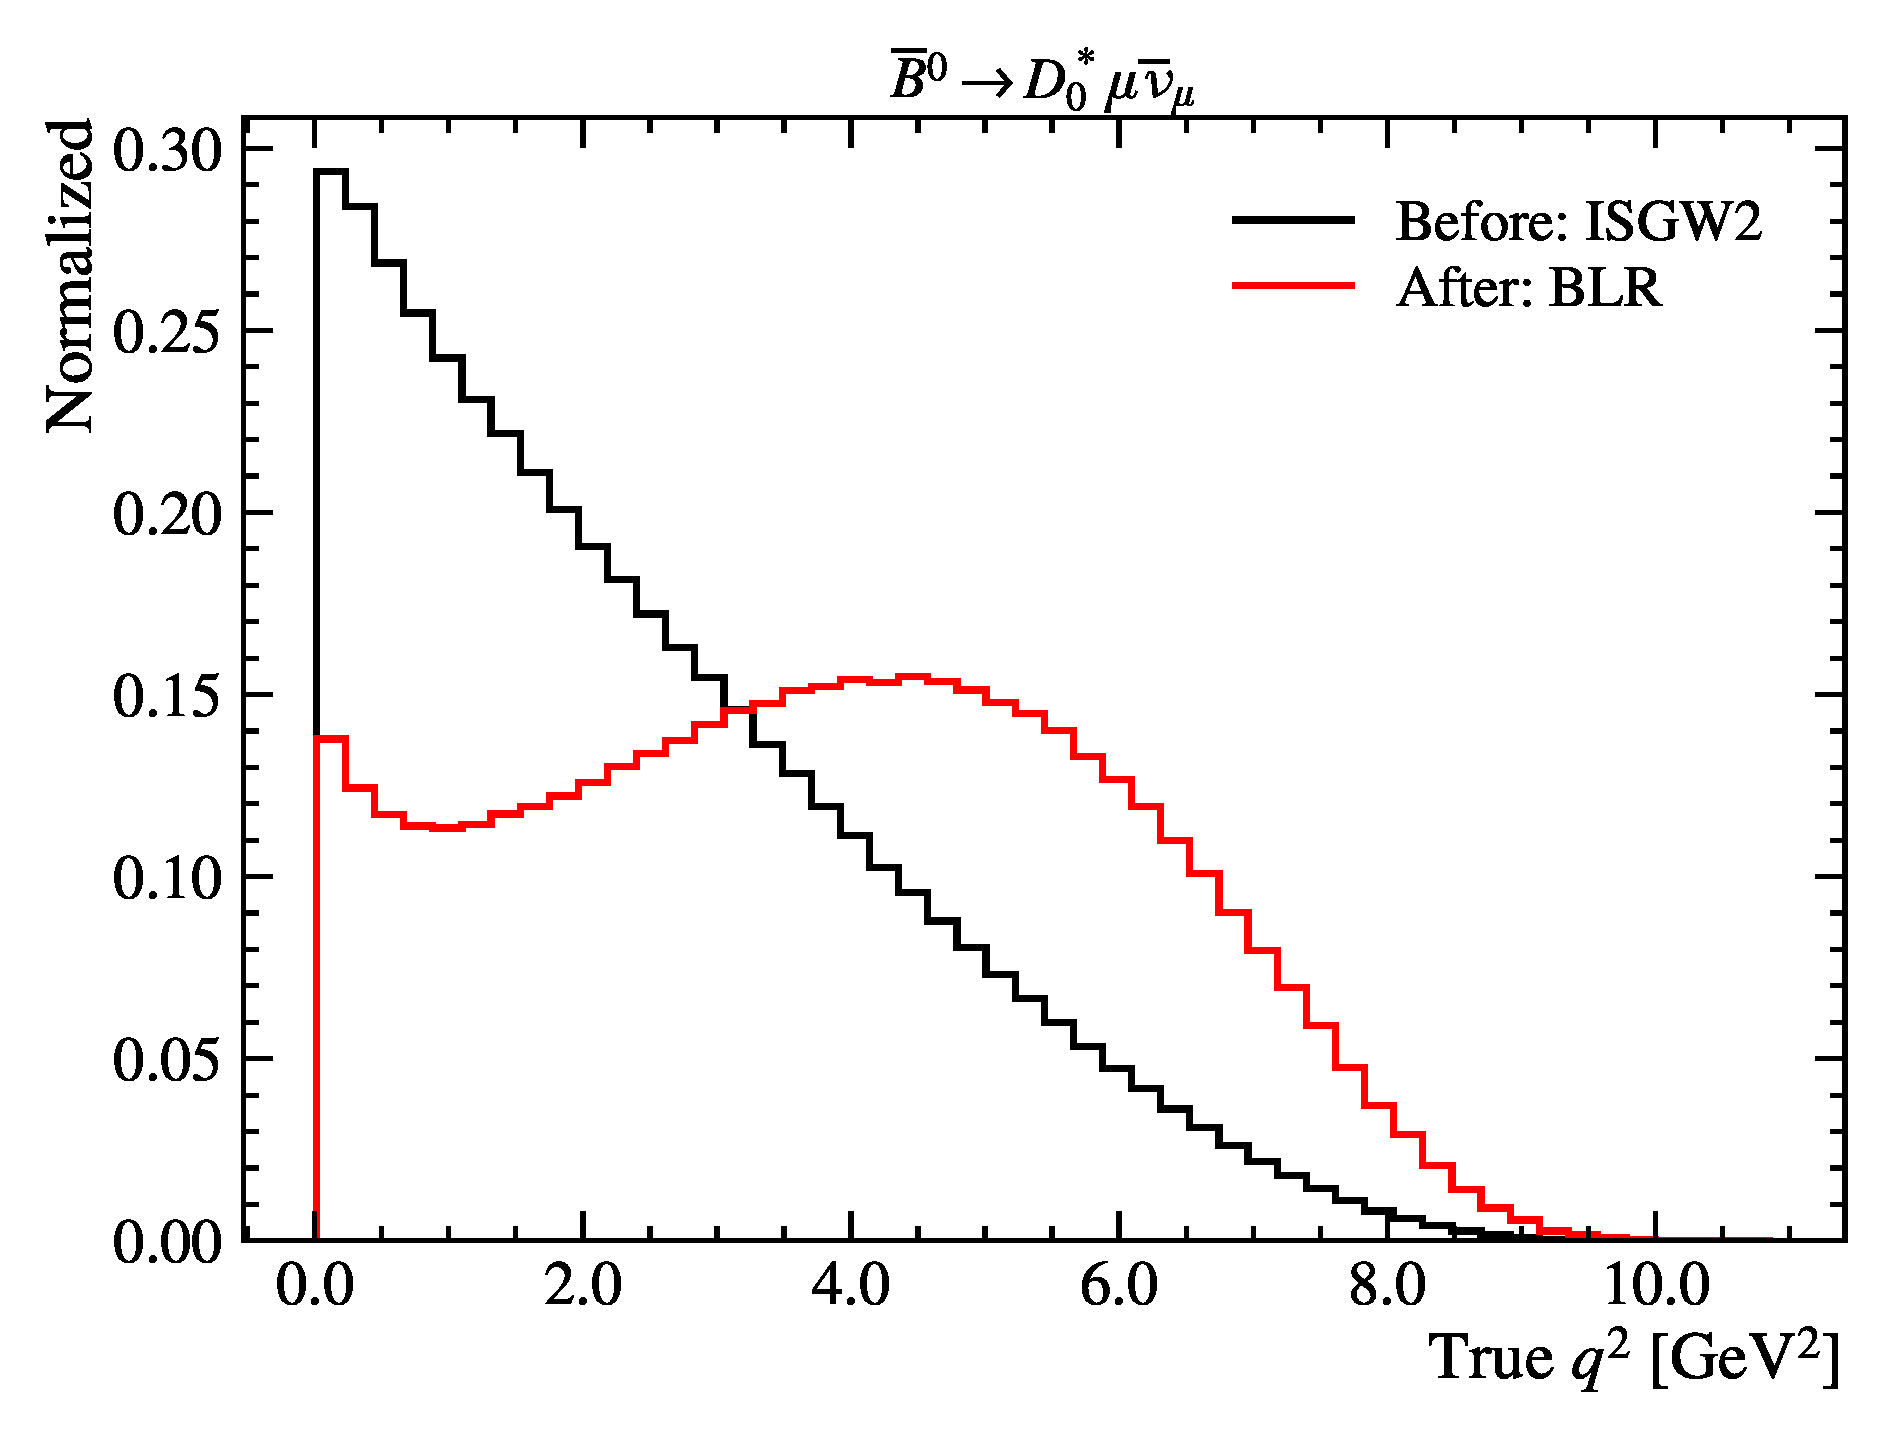
\includegraphics[width=0.24\textwidth]{
        ./figs-mc-correction/reweighting-form-factors/DststMu/D0ststMu.pdf
    }
    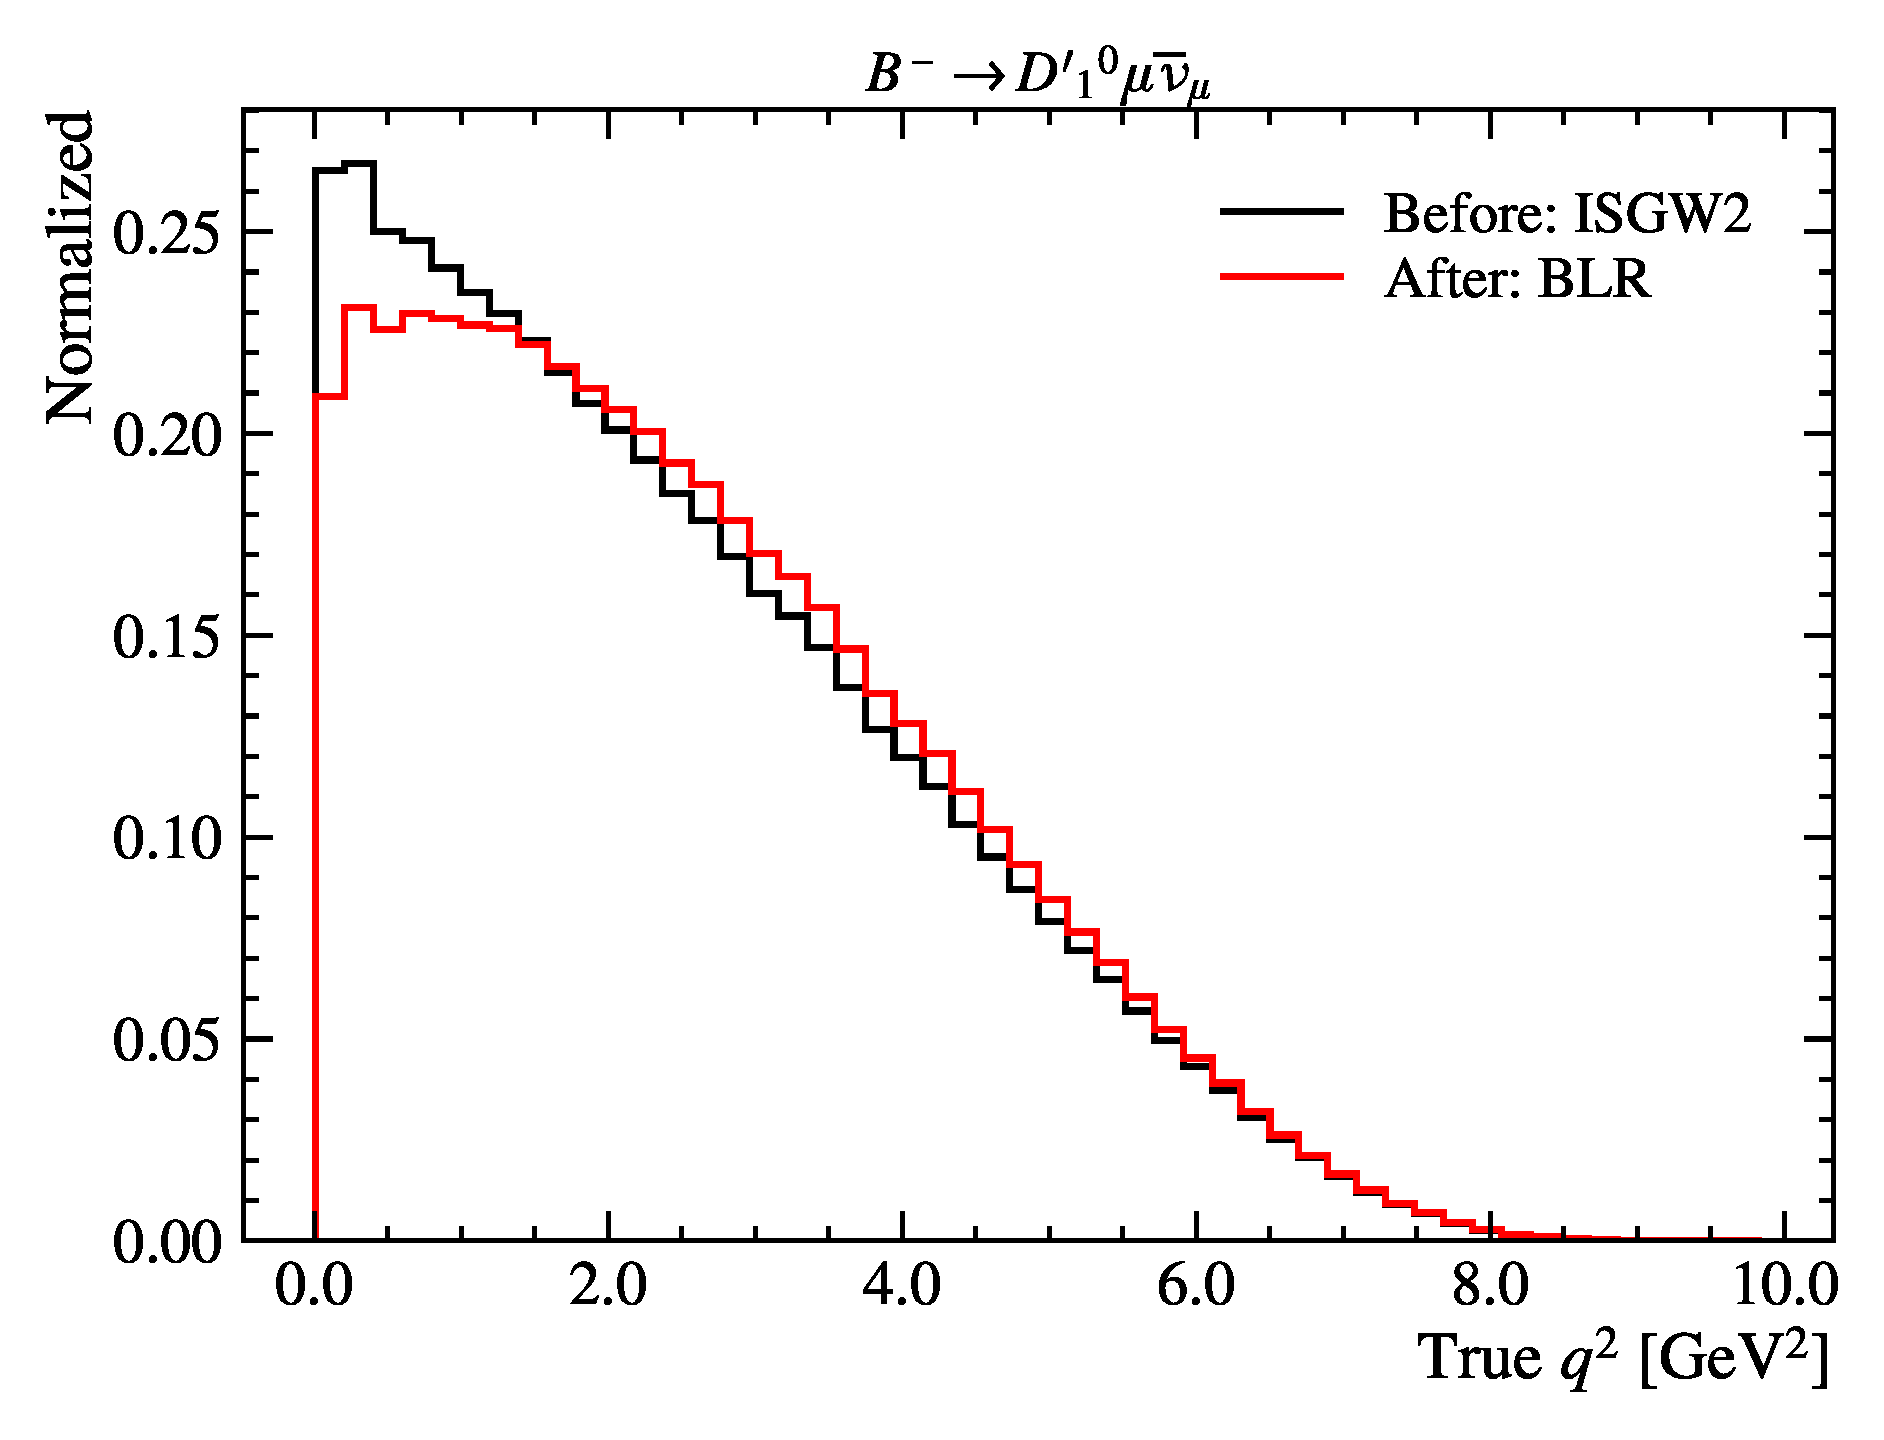
\includegraphics[width=0.24\textwidth]{
        ./figs-mc-correction/reweighting-form-factors/DststMu/D1pstst0Mu.pdf
    }
    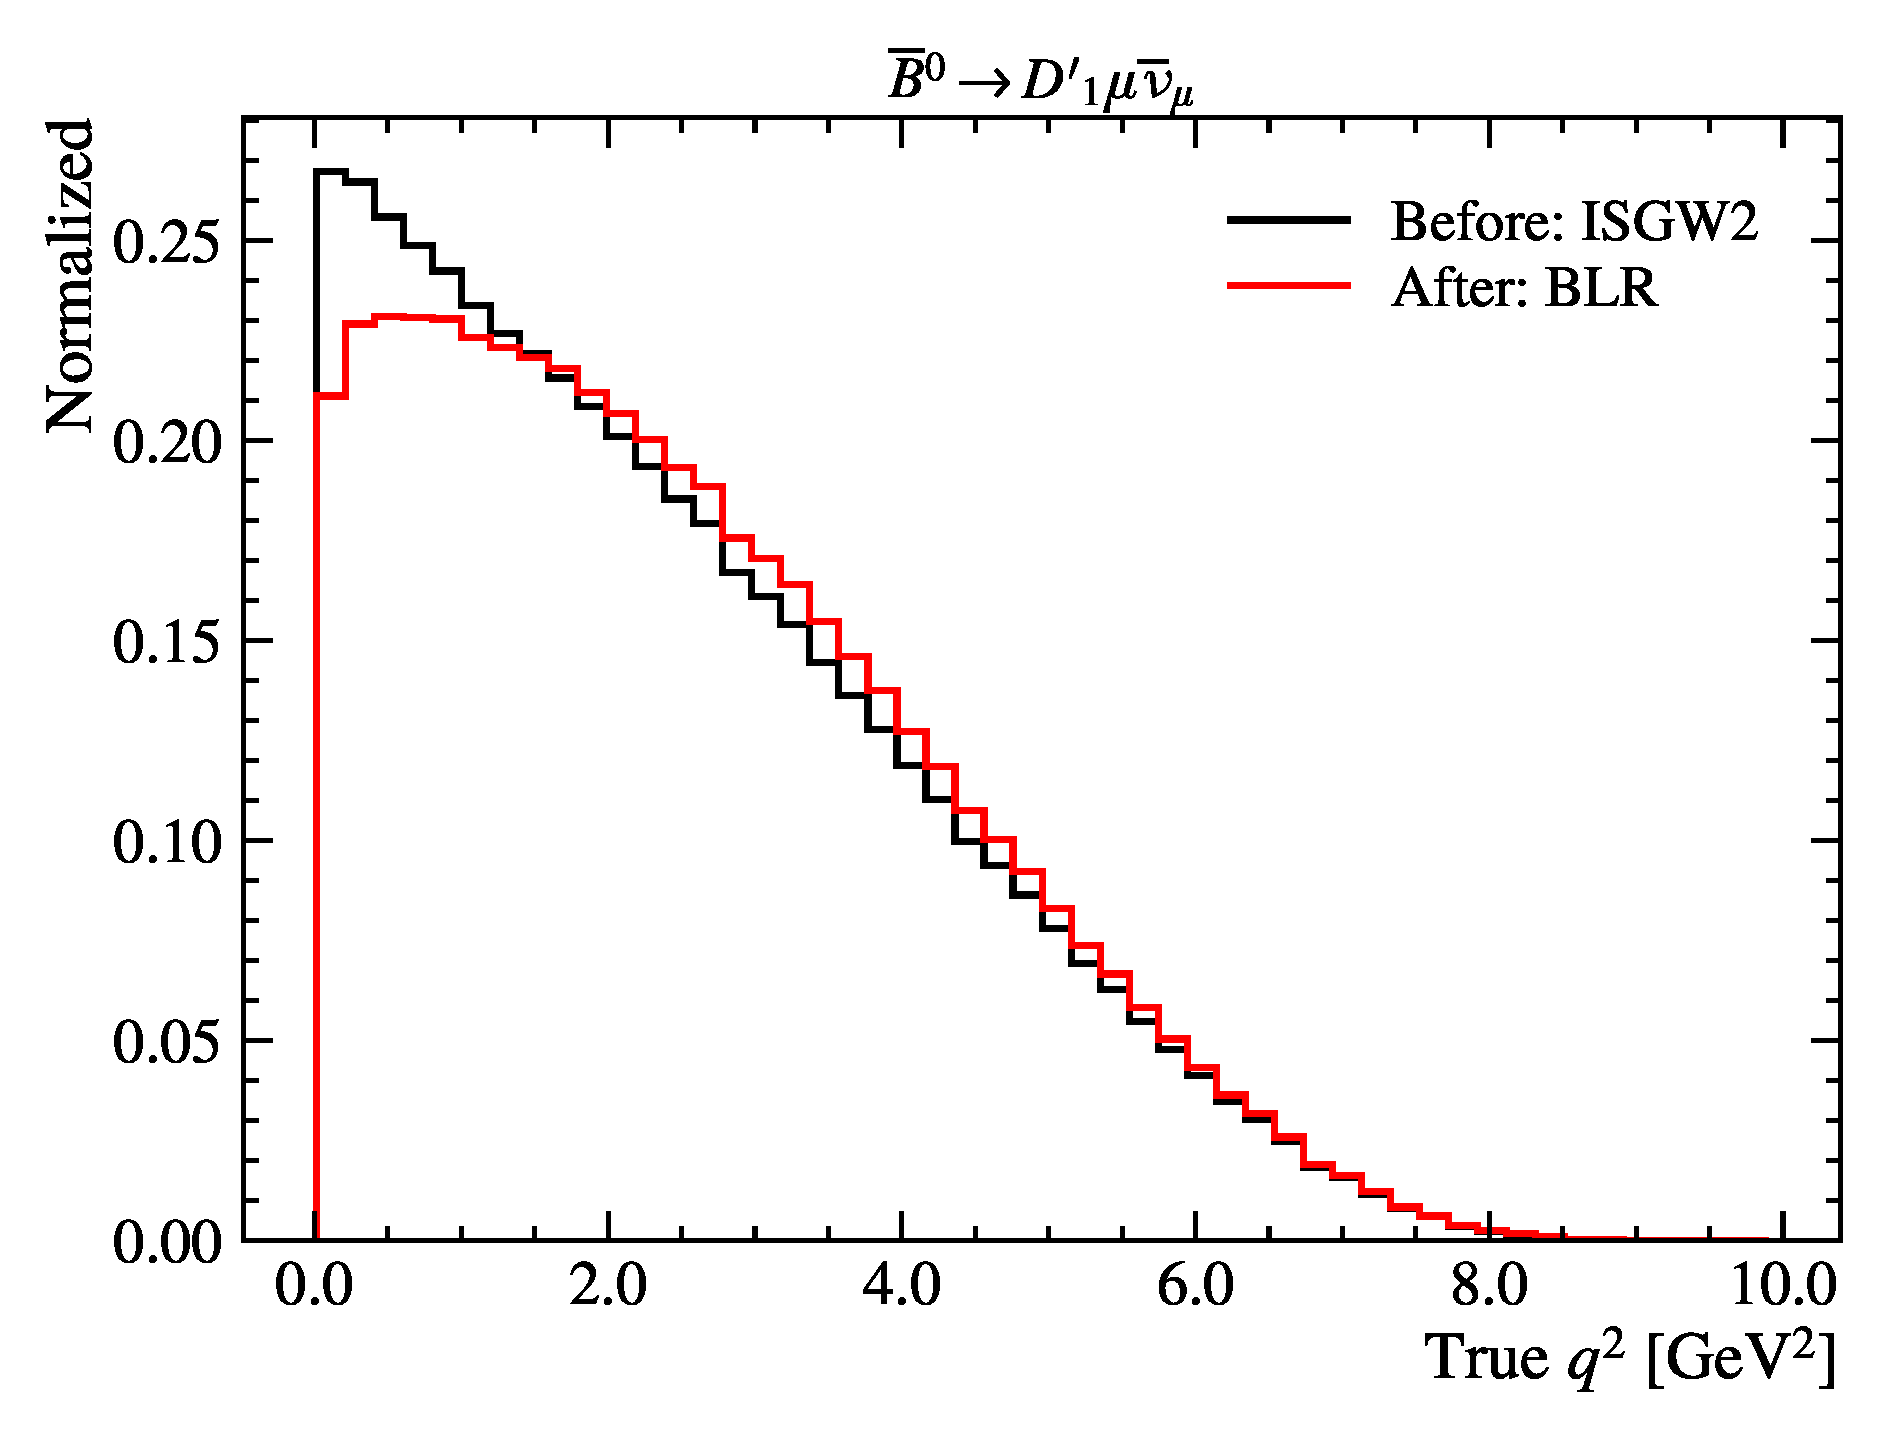
\includegraphics[width=0.24\textwidth]{
        ./figs-mc-correction/reweighting-form-factors/DststMu/D1pststMu.pdf
    }

    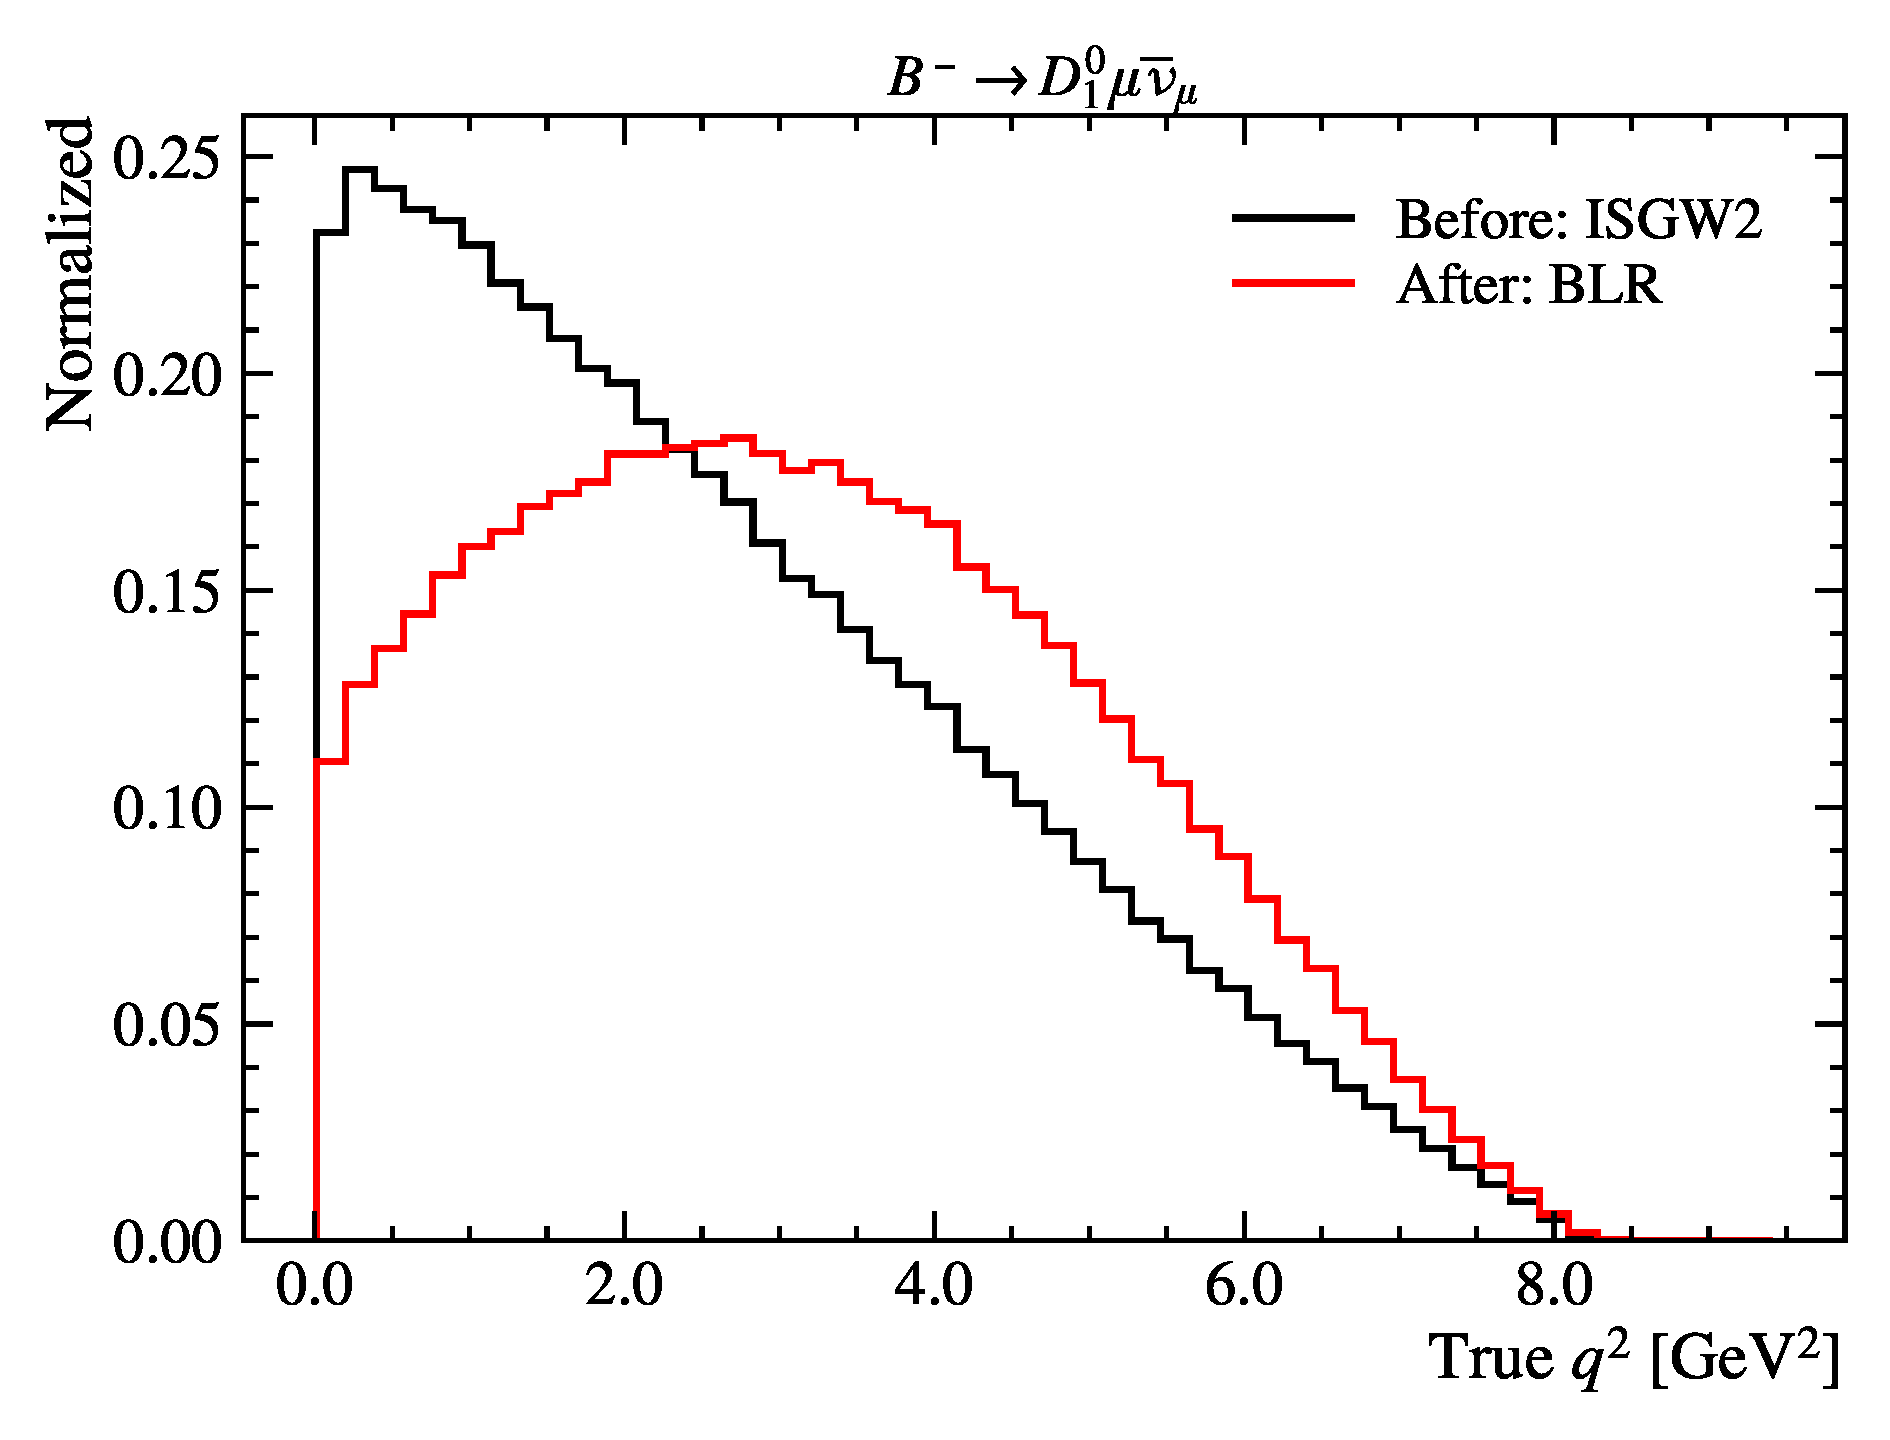
\includegraphics[width=0.24\textwidth]{
        ./figs-mc-correction/reweighting-form-factors/DststMu/D1stst0Mu.pdf
    }
    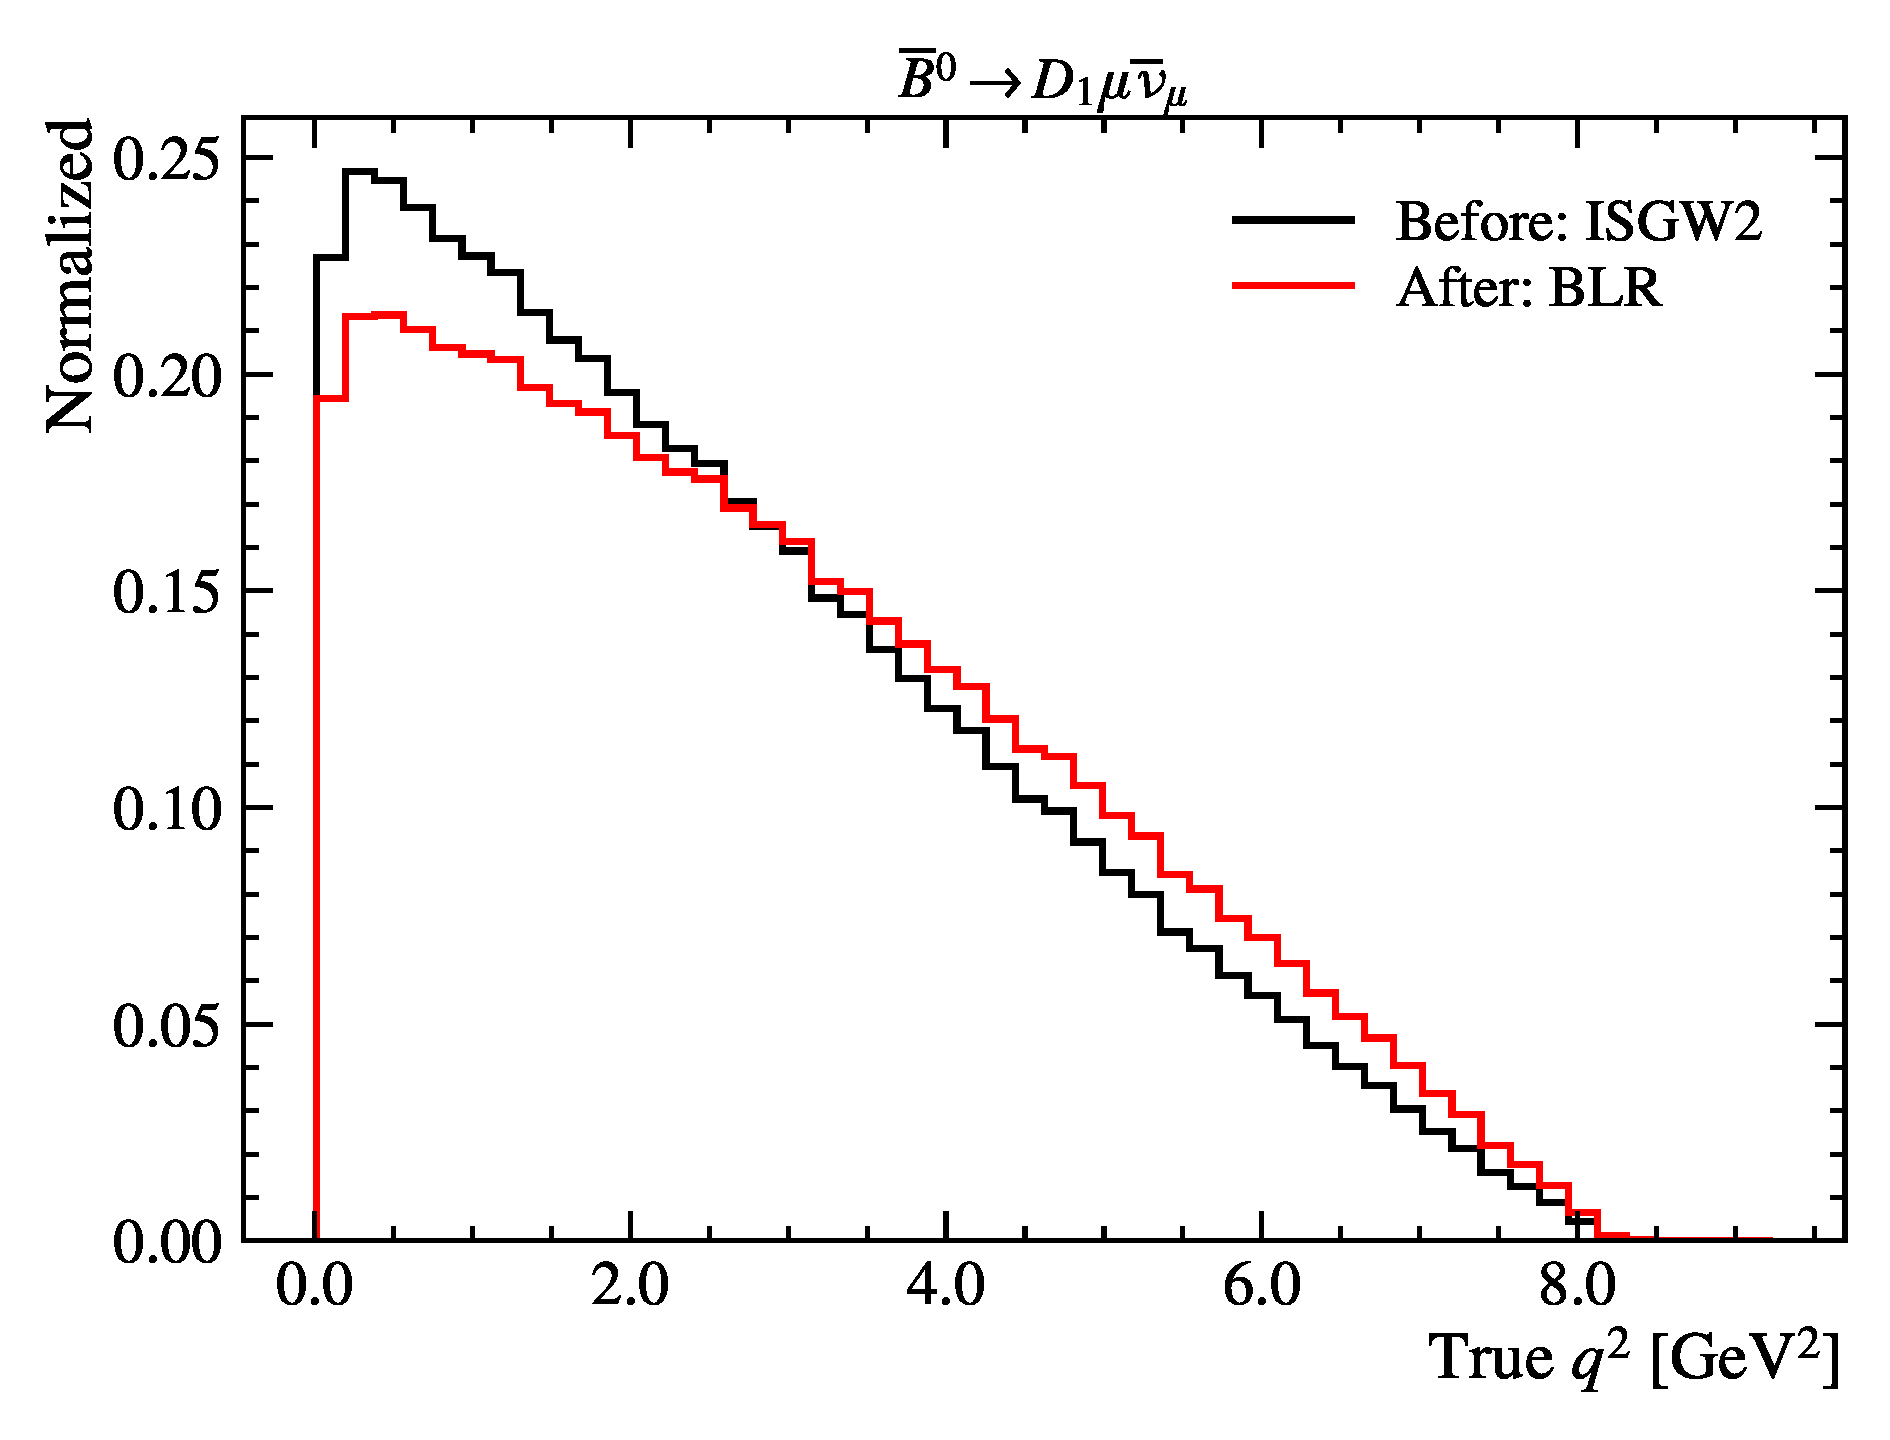
\includegraphics[width=0.24\textwidth]{
        ./figs-mc-correction/reweighting-form-factors/DststMu/D1ststMu.pdf
    }
    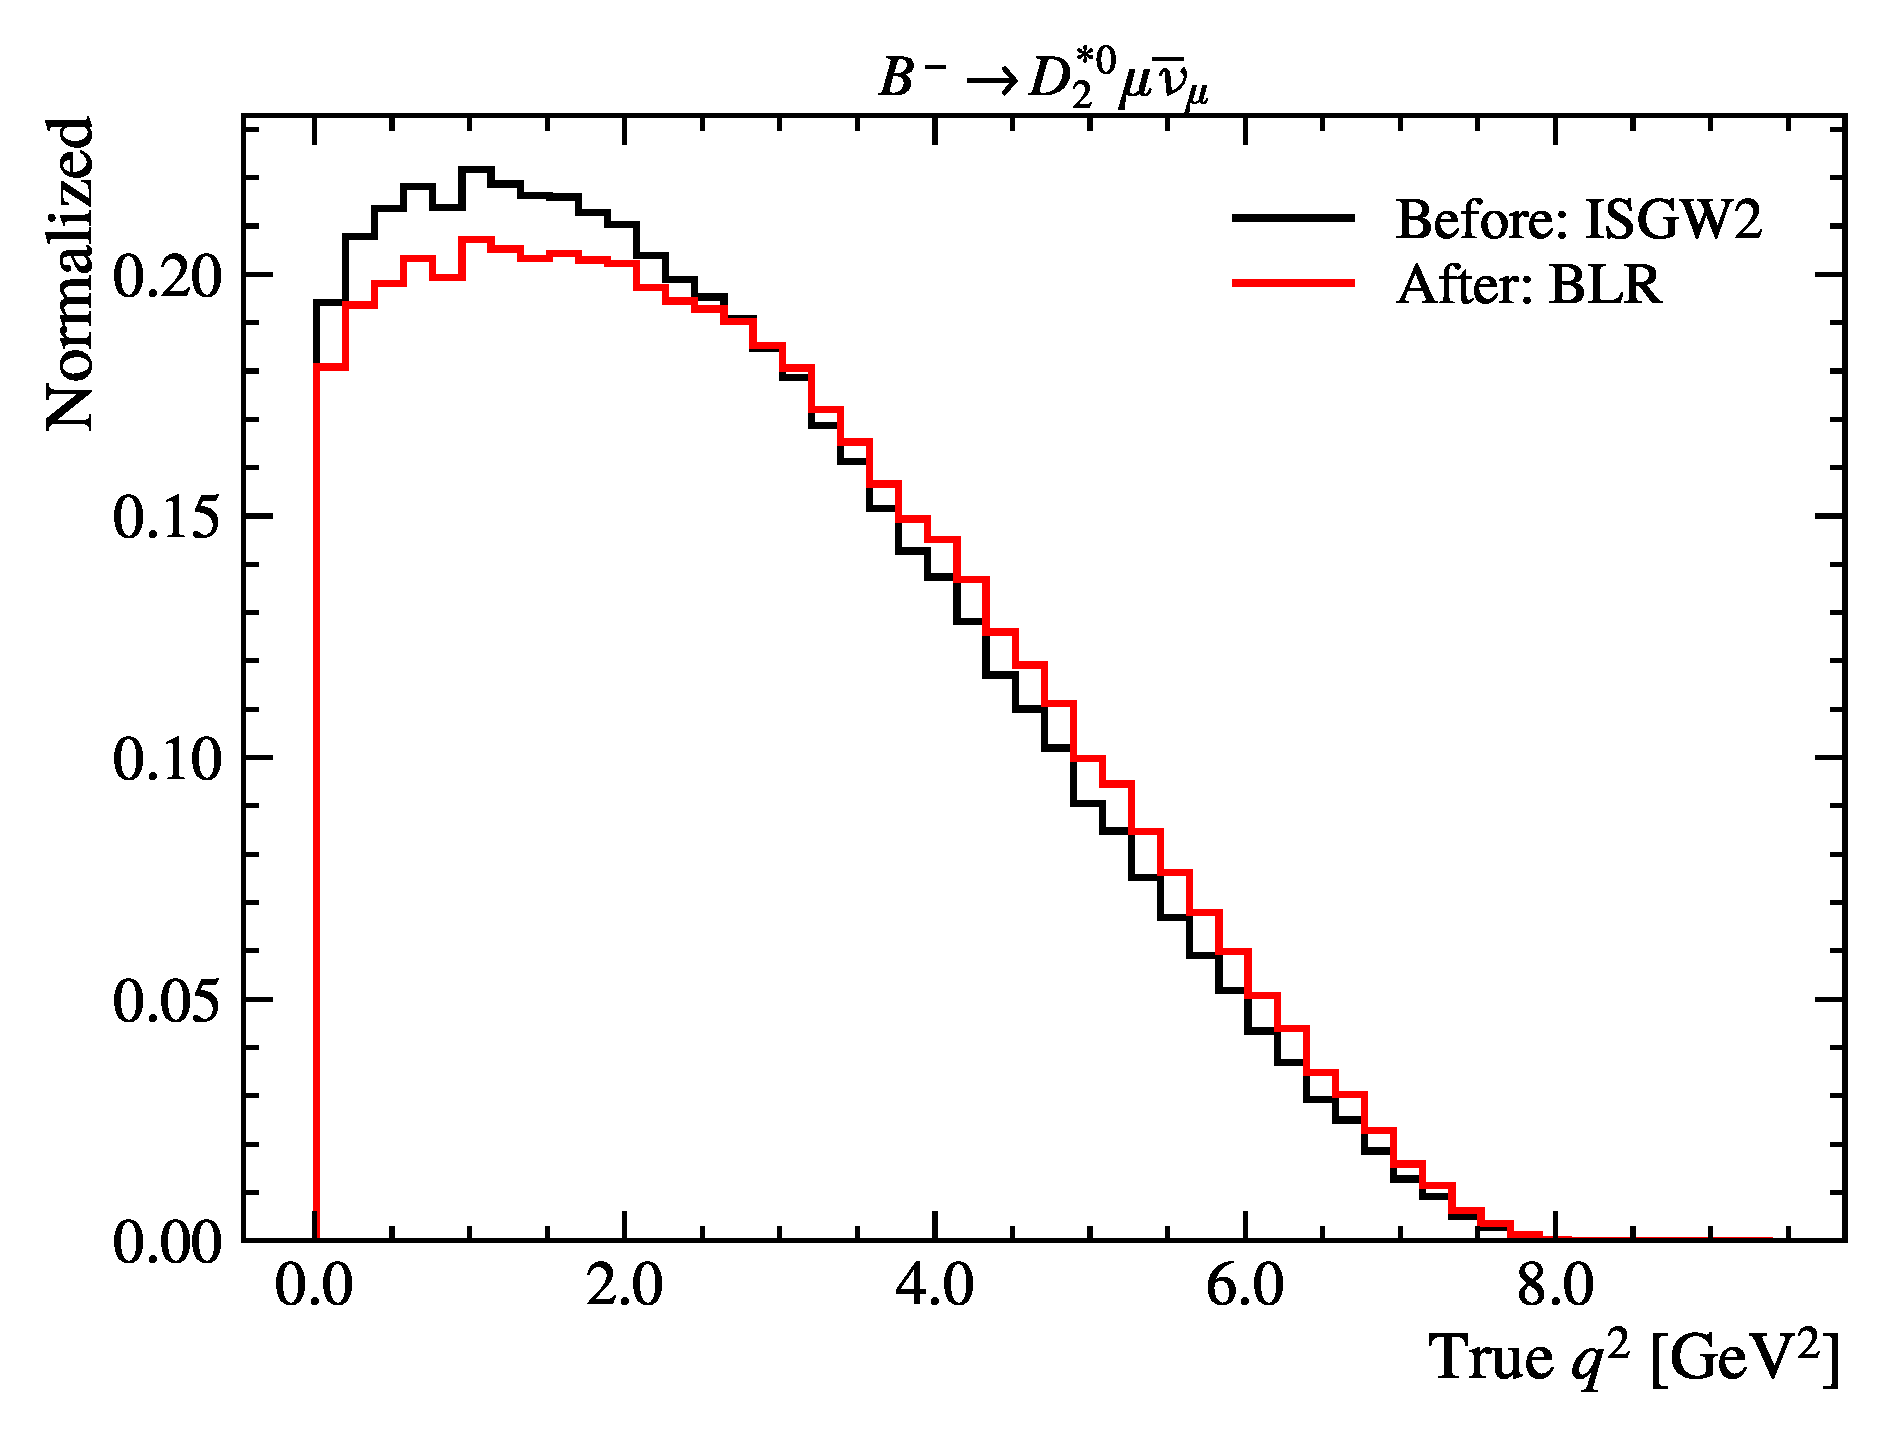
\includegraphics[width=0.24\textwidth]{
        ./figs-mc-correction/reweighting-form-factors/DststMu/D2stst0Mu.pdf
    }
    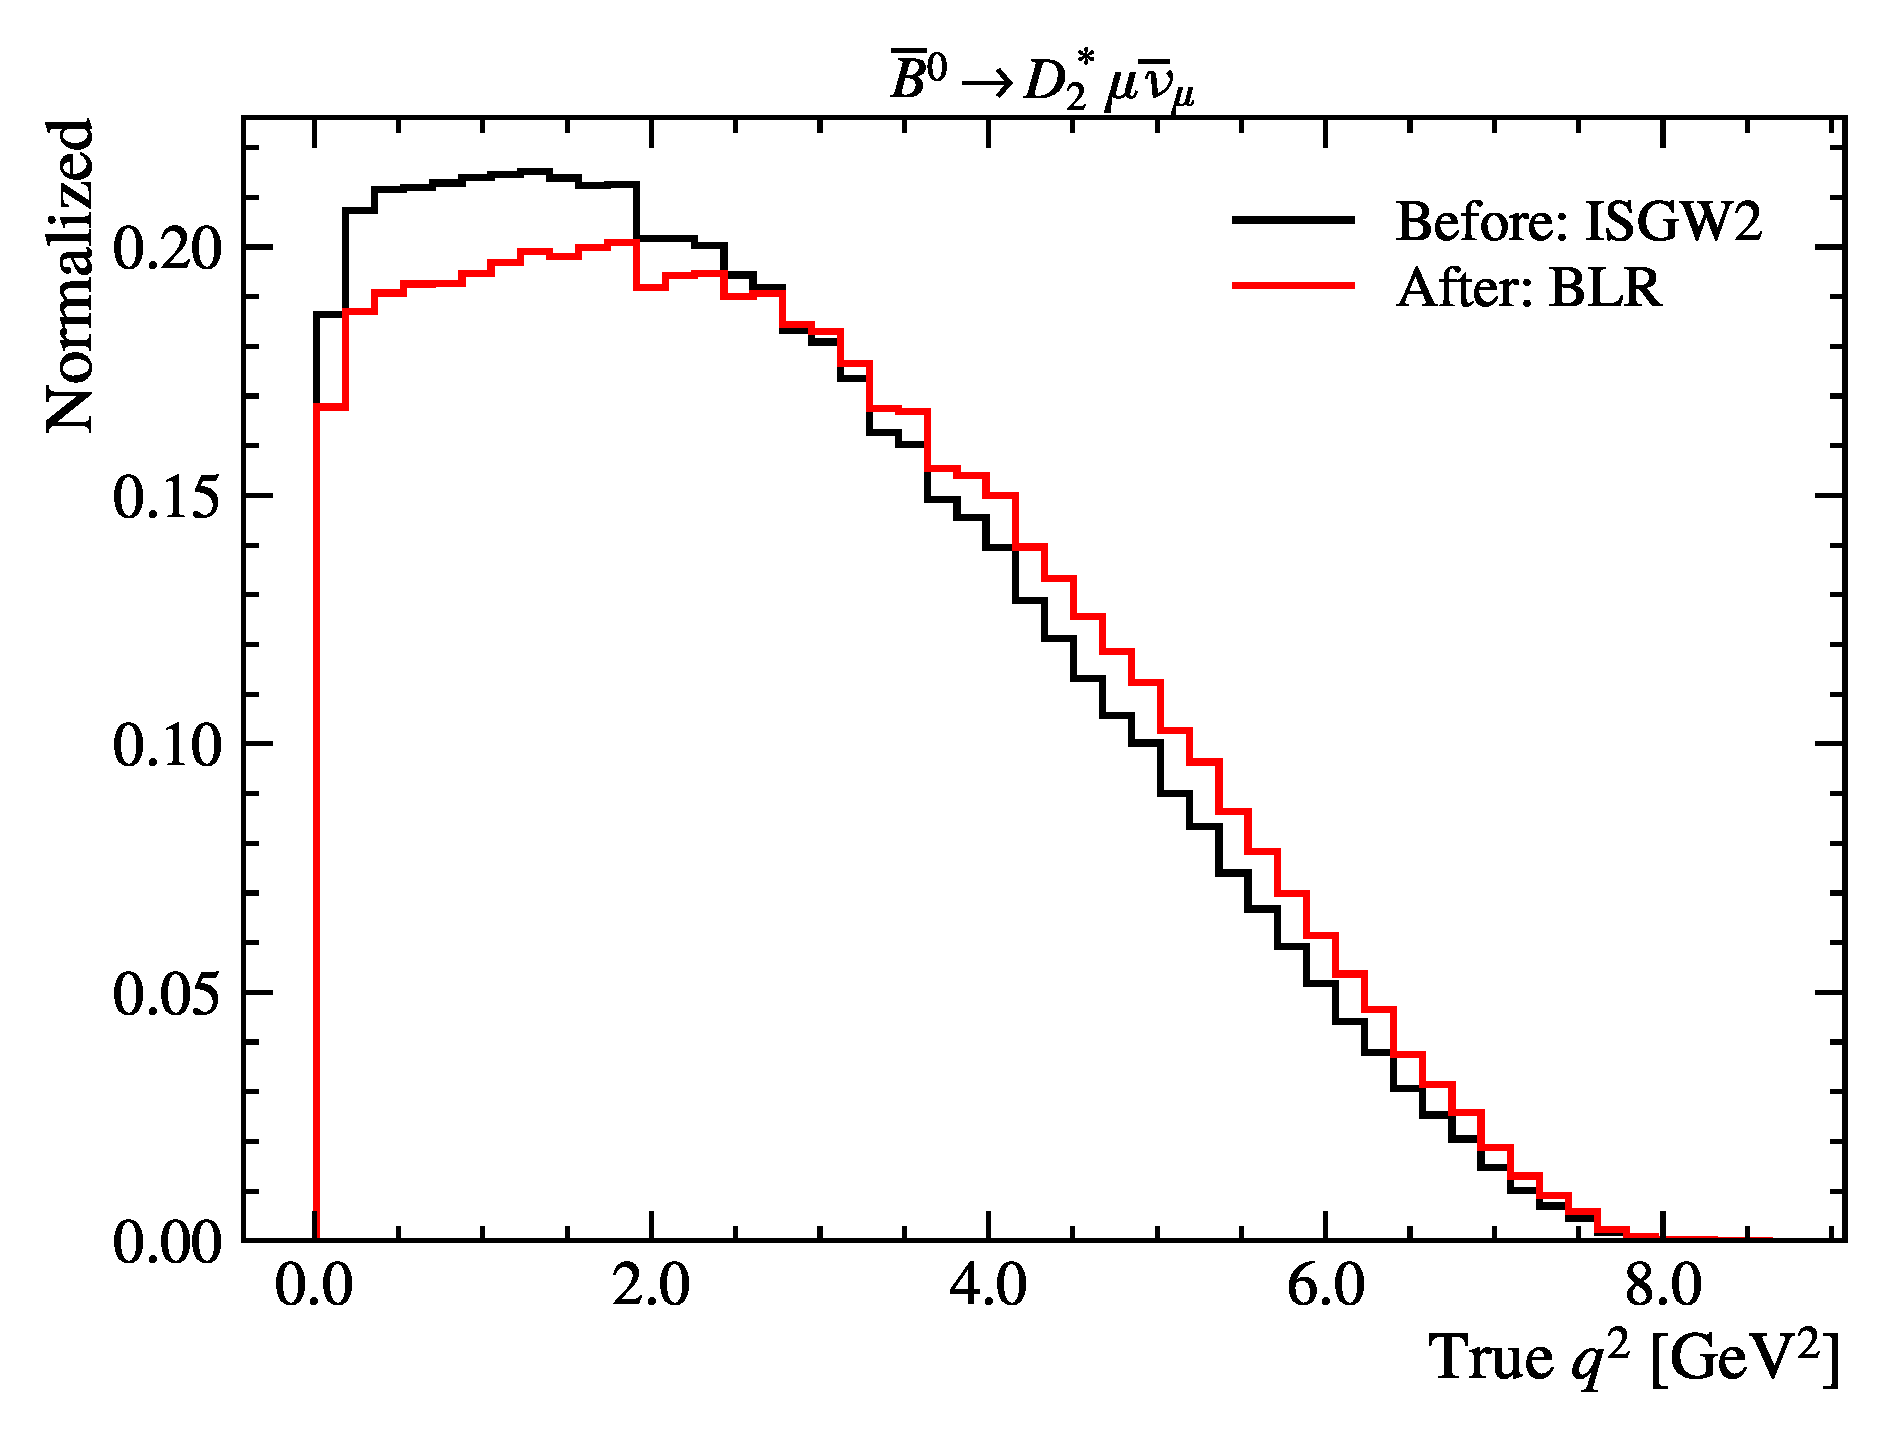
\includegraphics[width=0.24\textwidth]{
        ./figs-mc-correction/reweighting-form-factors/DststMu/D2ststMu.pdf
    }

    \caption{
        Form factor reweight effect on $D^{**}\mu$ MC templates.
        Parameters are shifted based an initial fit.
    }
    \label{fig:ff-rwt-Dstst-norm-like}
\end{figure}

\begin{figure}[ht]
    \centering
    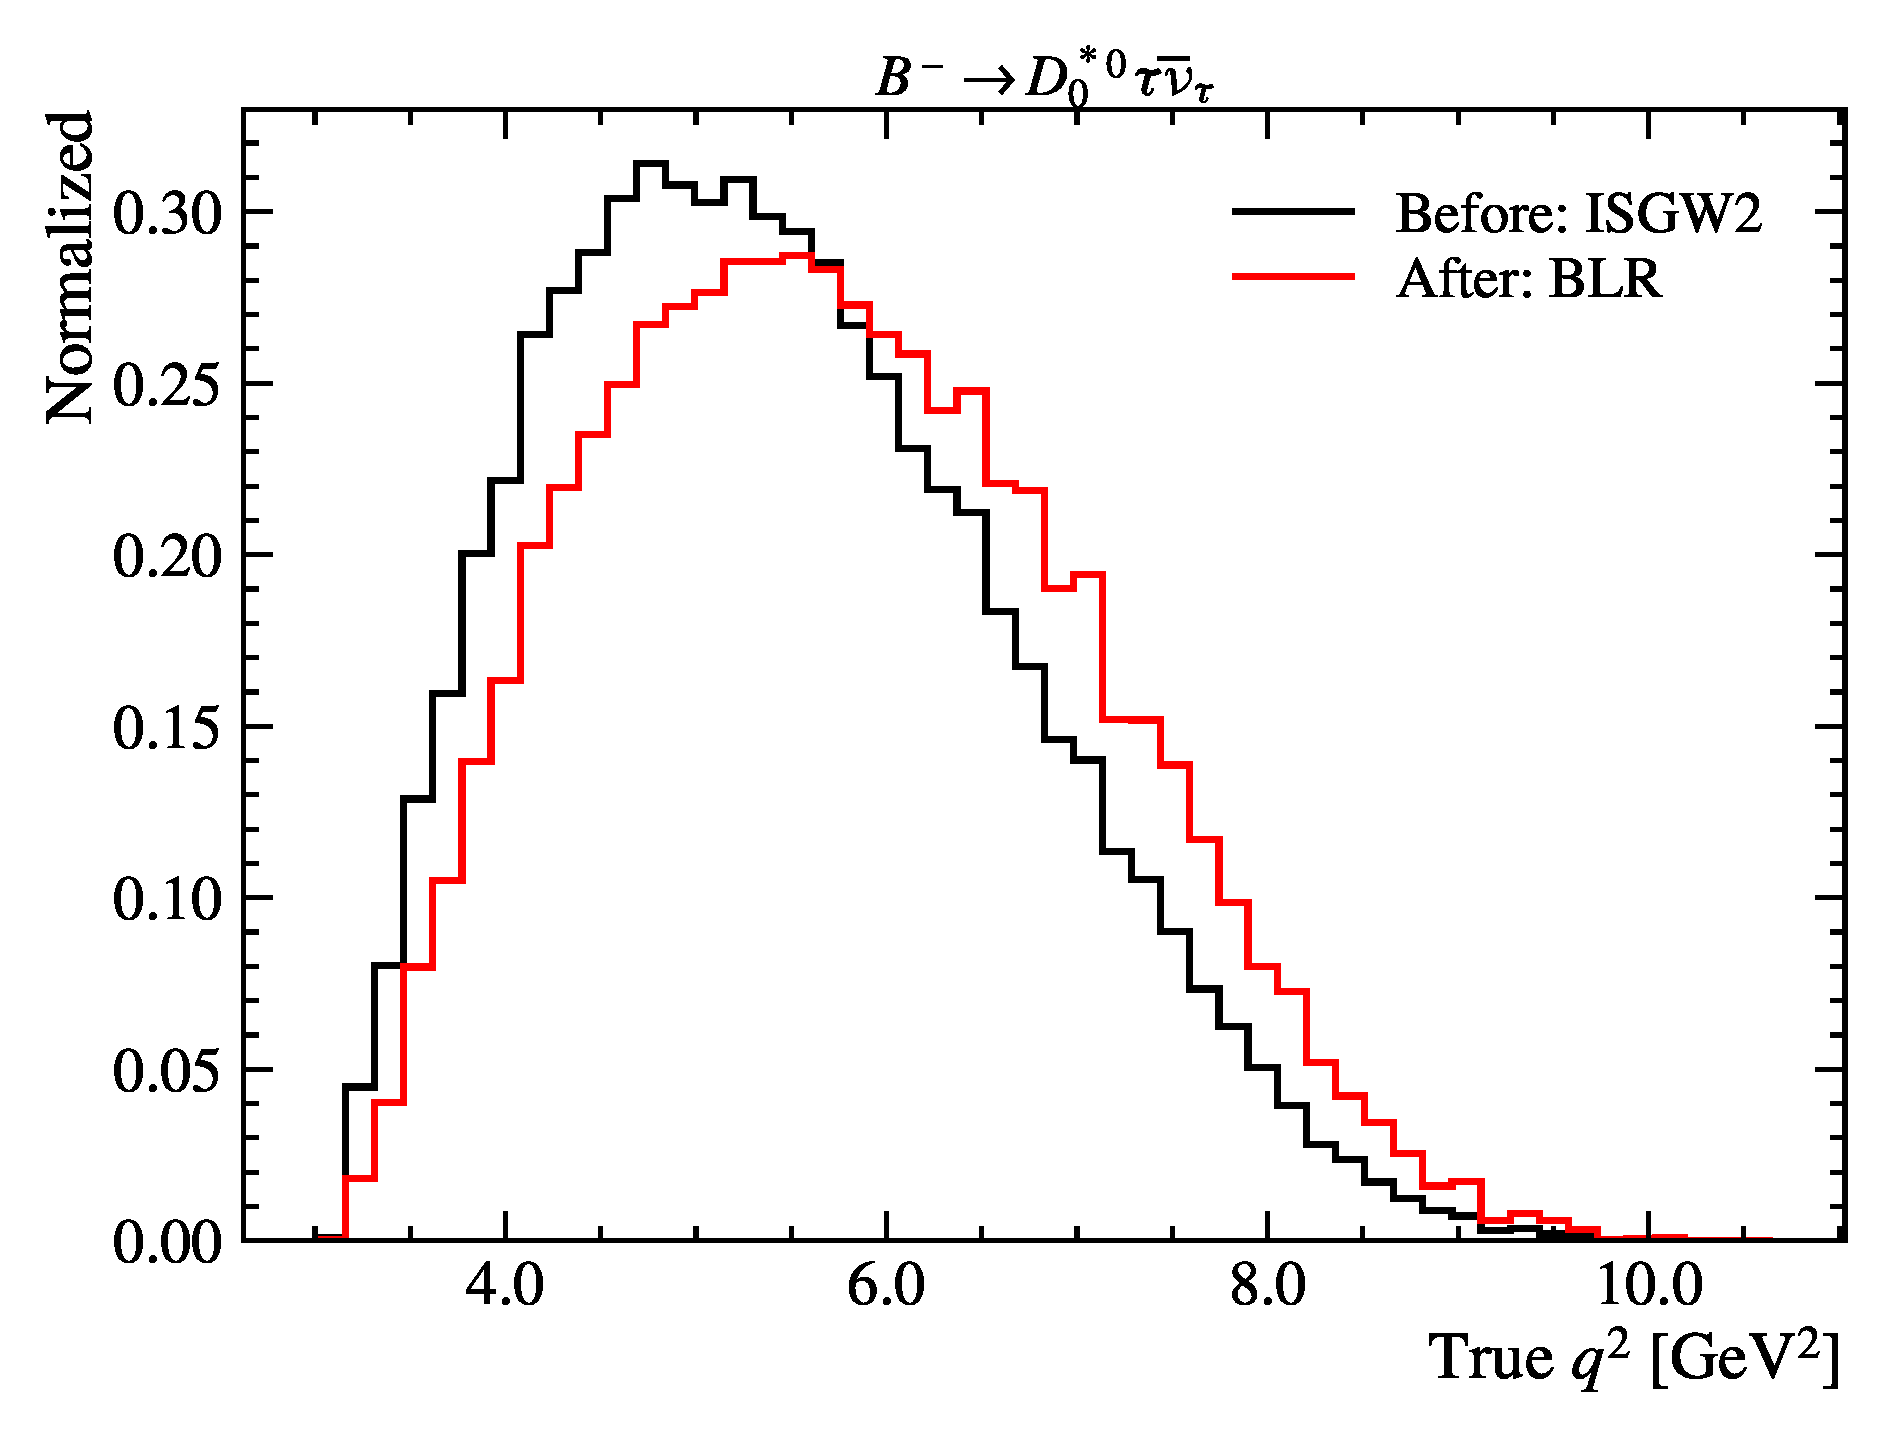
\includegraphics[width=0.24\textwidth]{
        ./figs-mc-correction/reweighting-form-factors/DststTau/D0stst0Tau.pdf
    }
    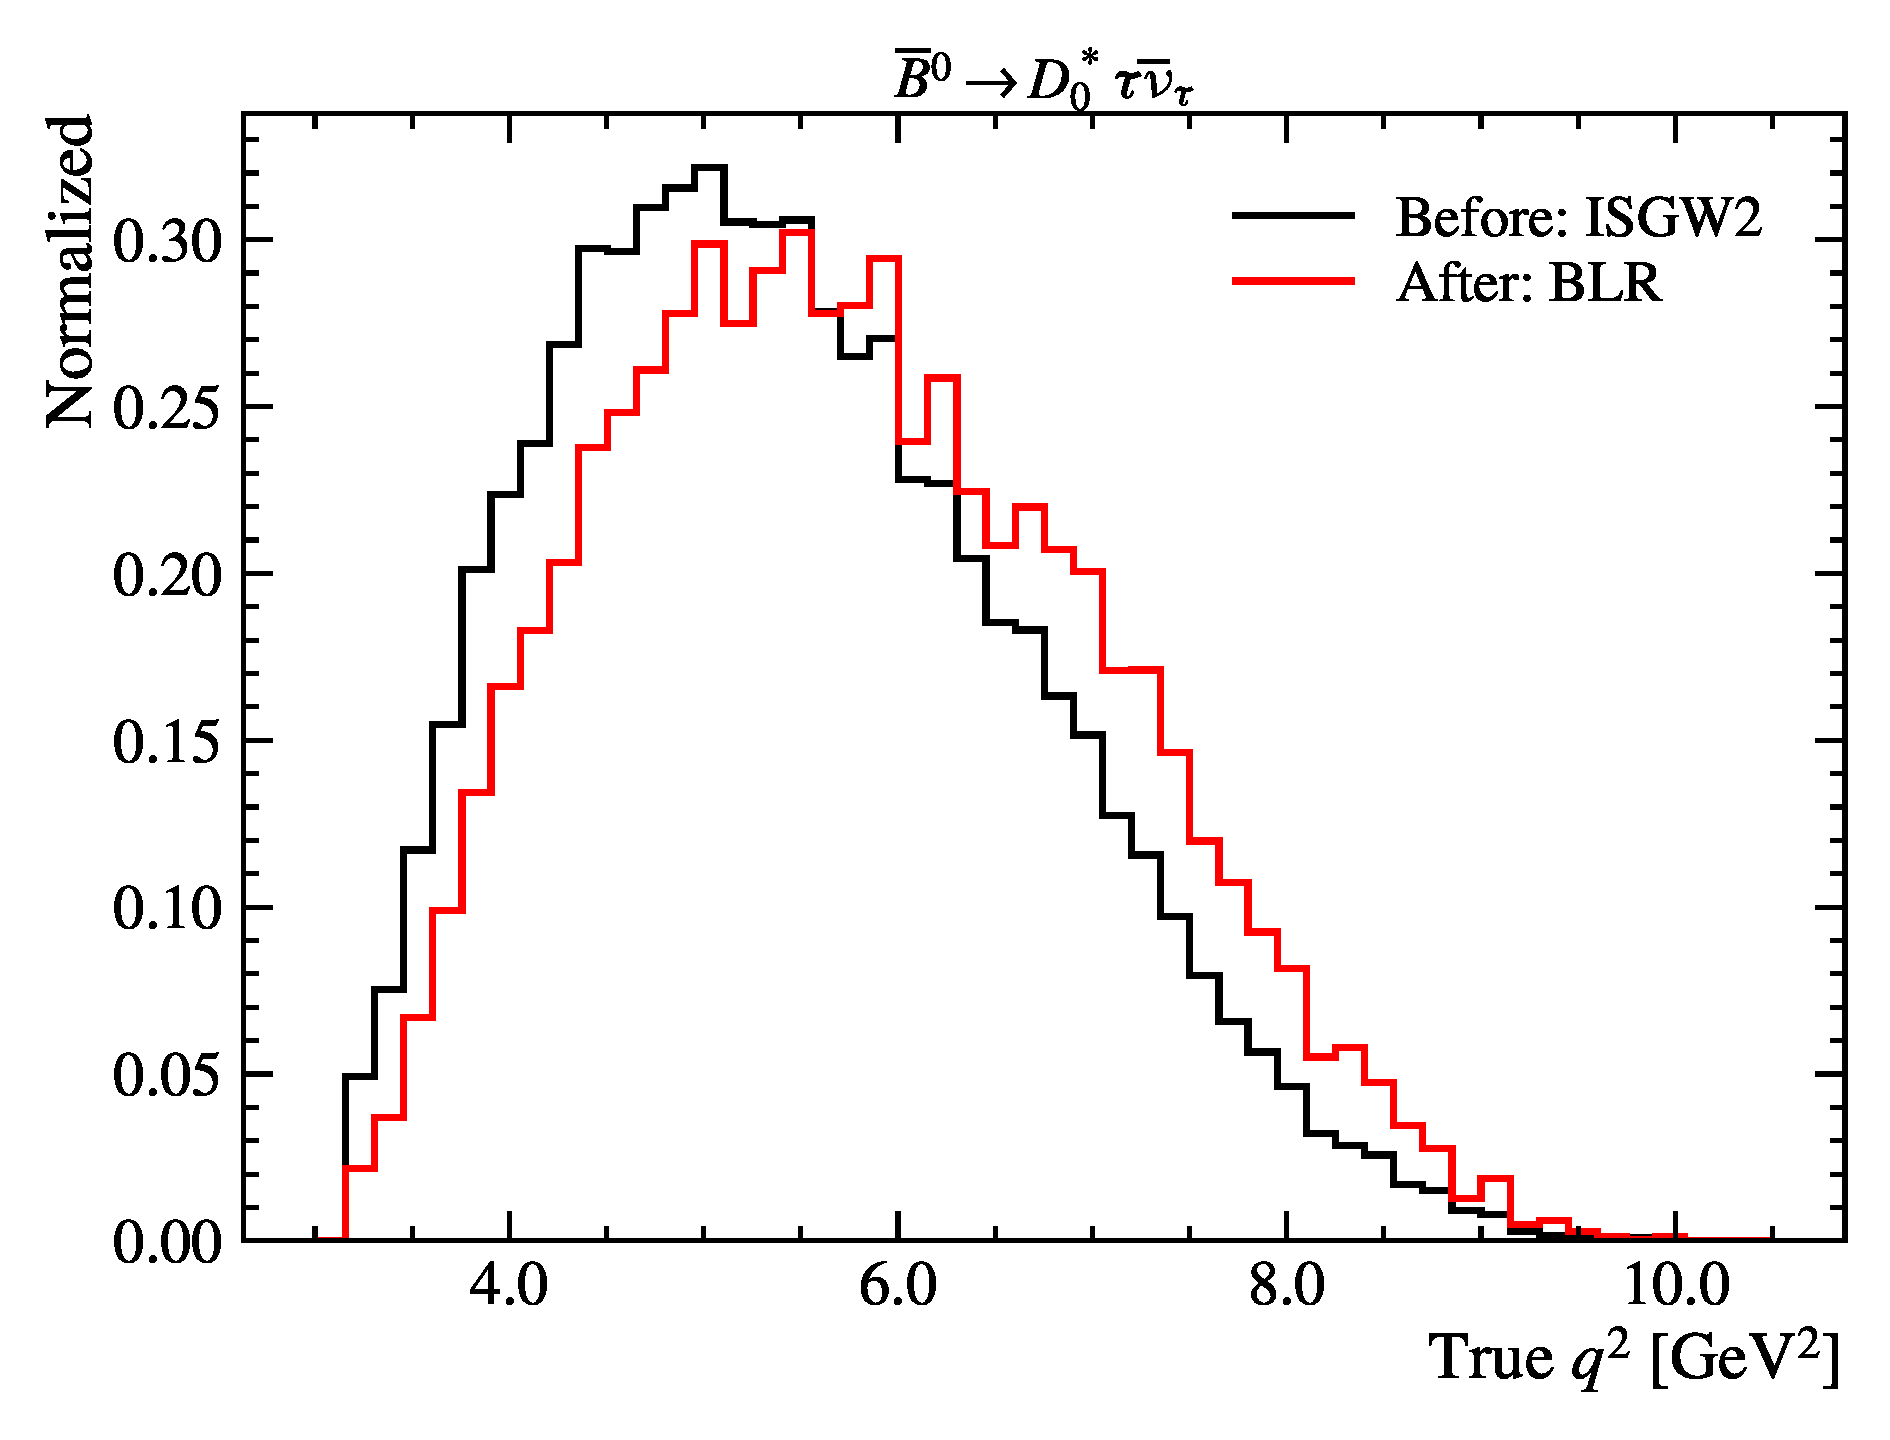
\includegraphics[width=0.24\textwidth]{
        ./figs-mc-correction/reweighting-form-factors/DststTau/D0ststTau.pdf
    }
    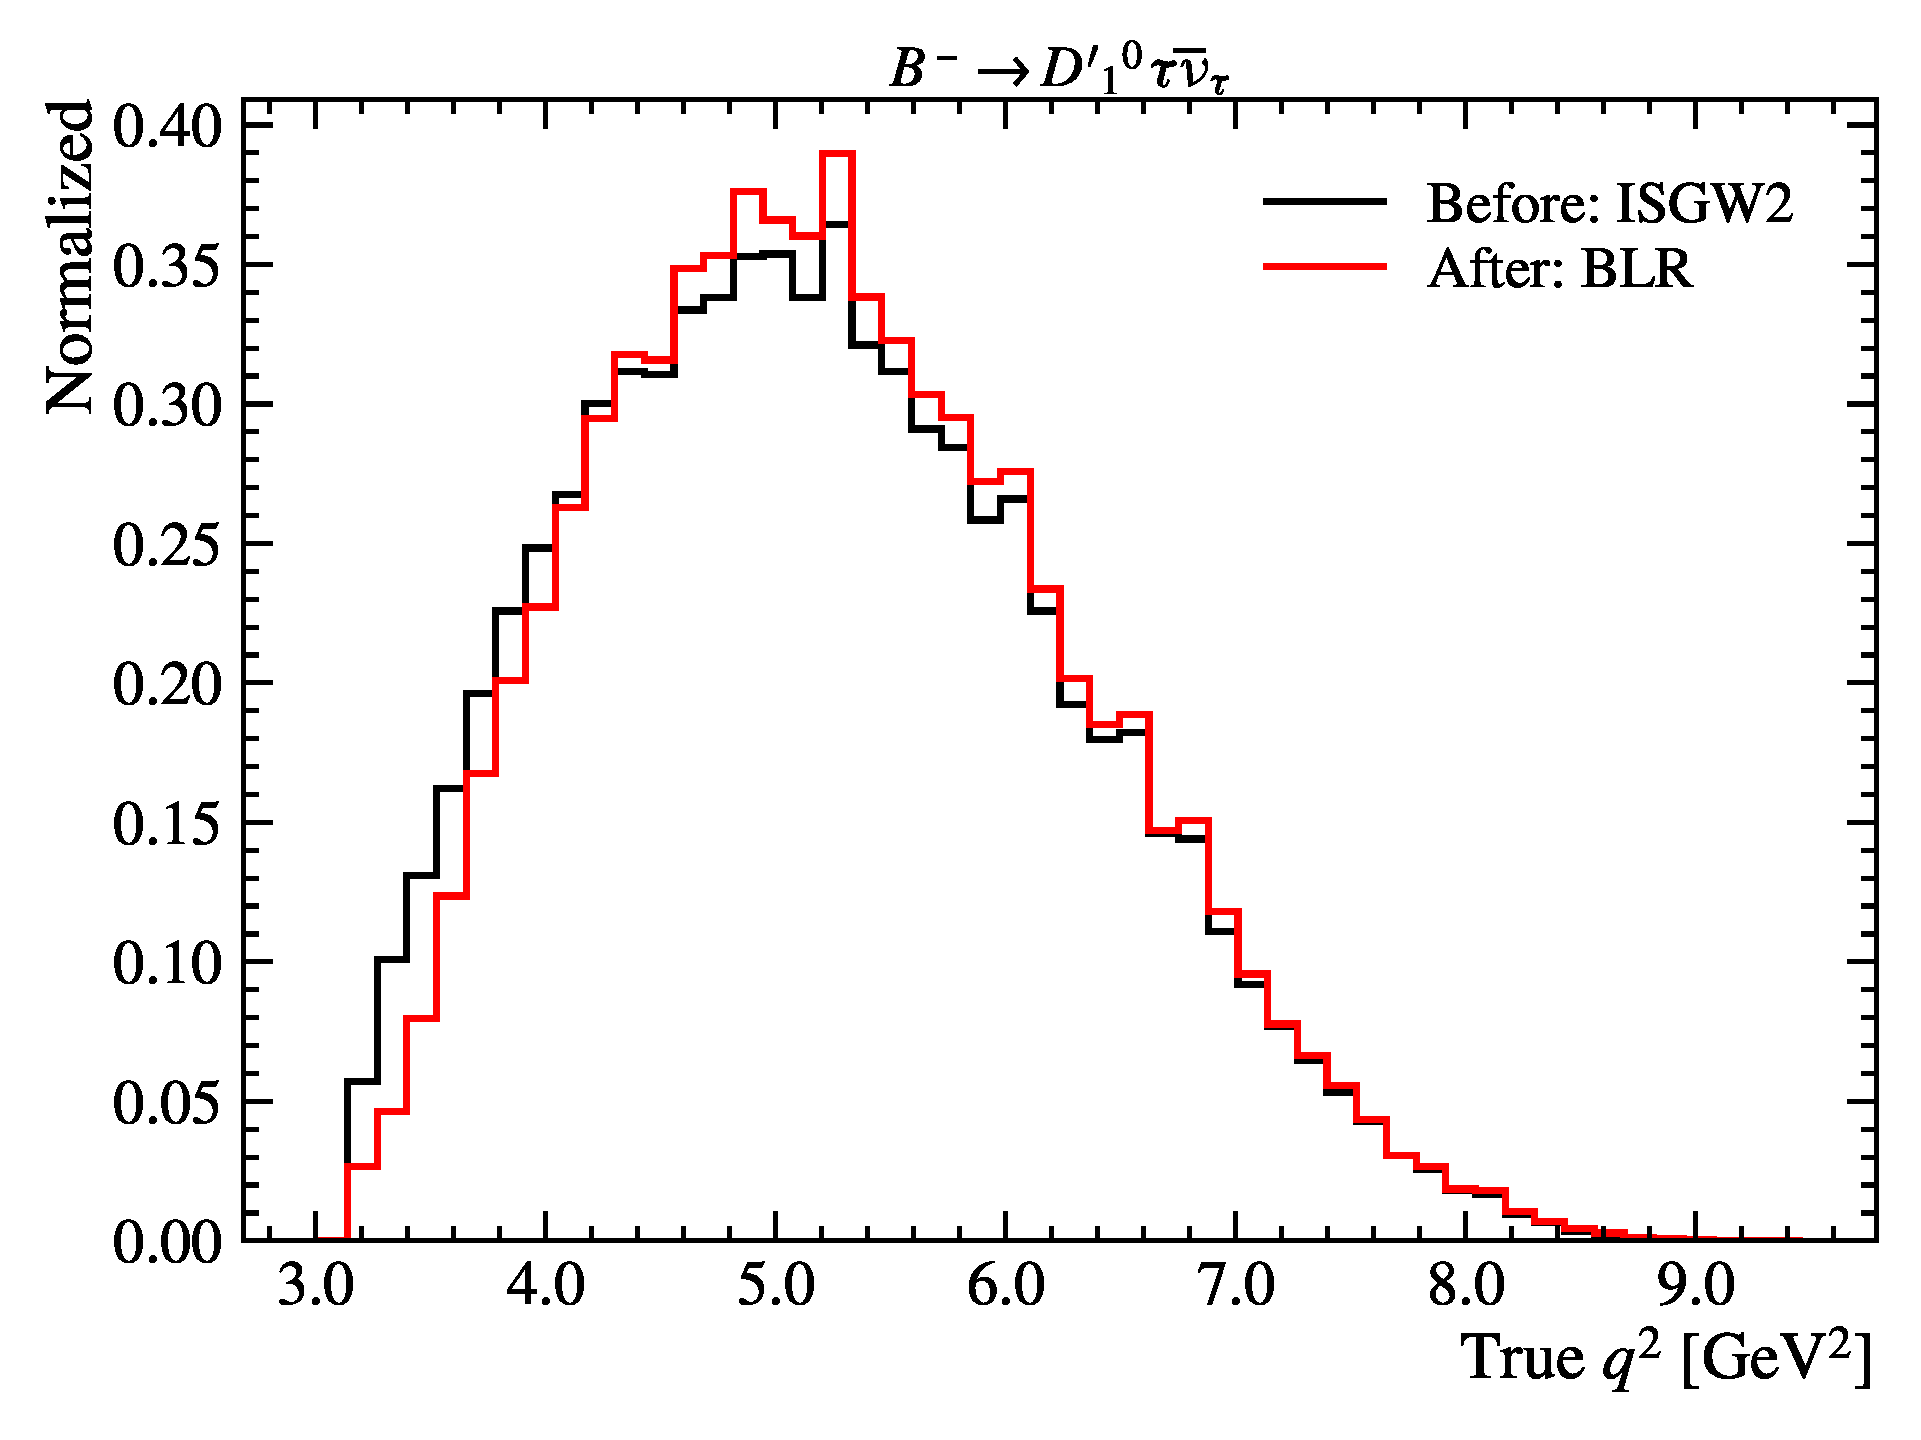
\includegraphics[width=0.24\textwidth]{
        ./figs-mc-correction/reweighting-form-factors/DststTau/D1pstst0Tau.pdf
    }
    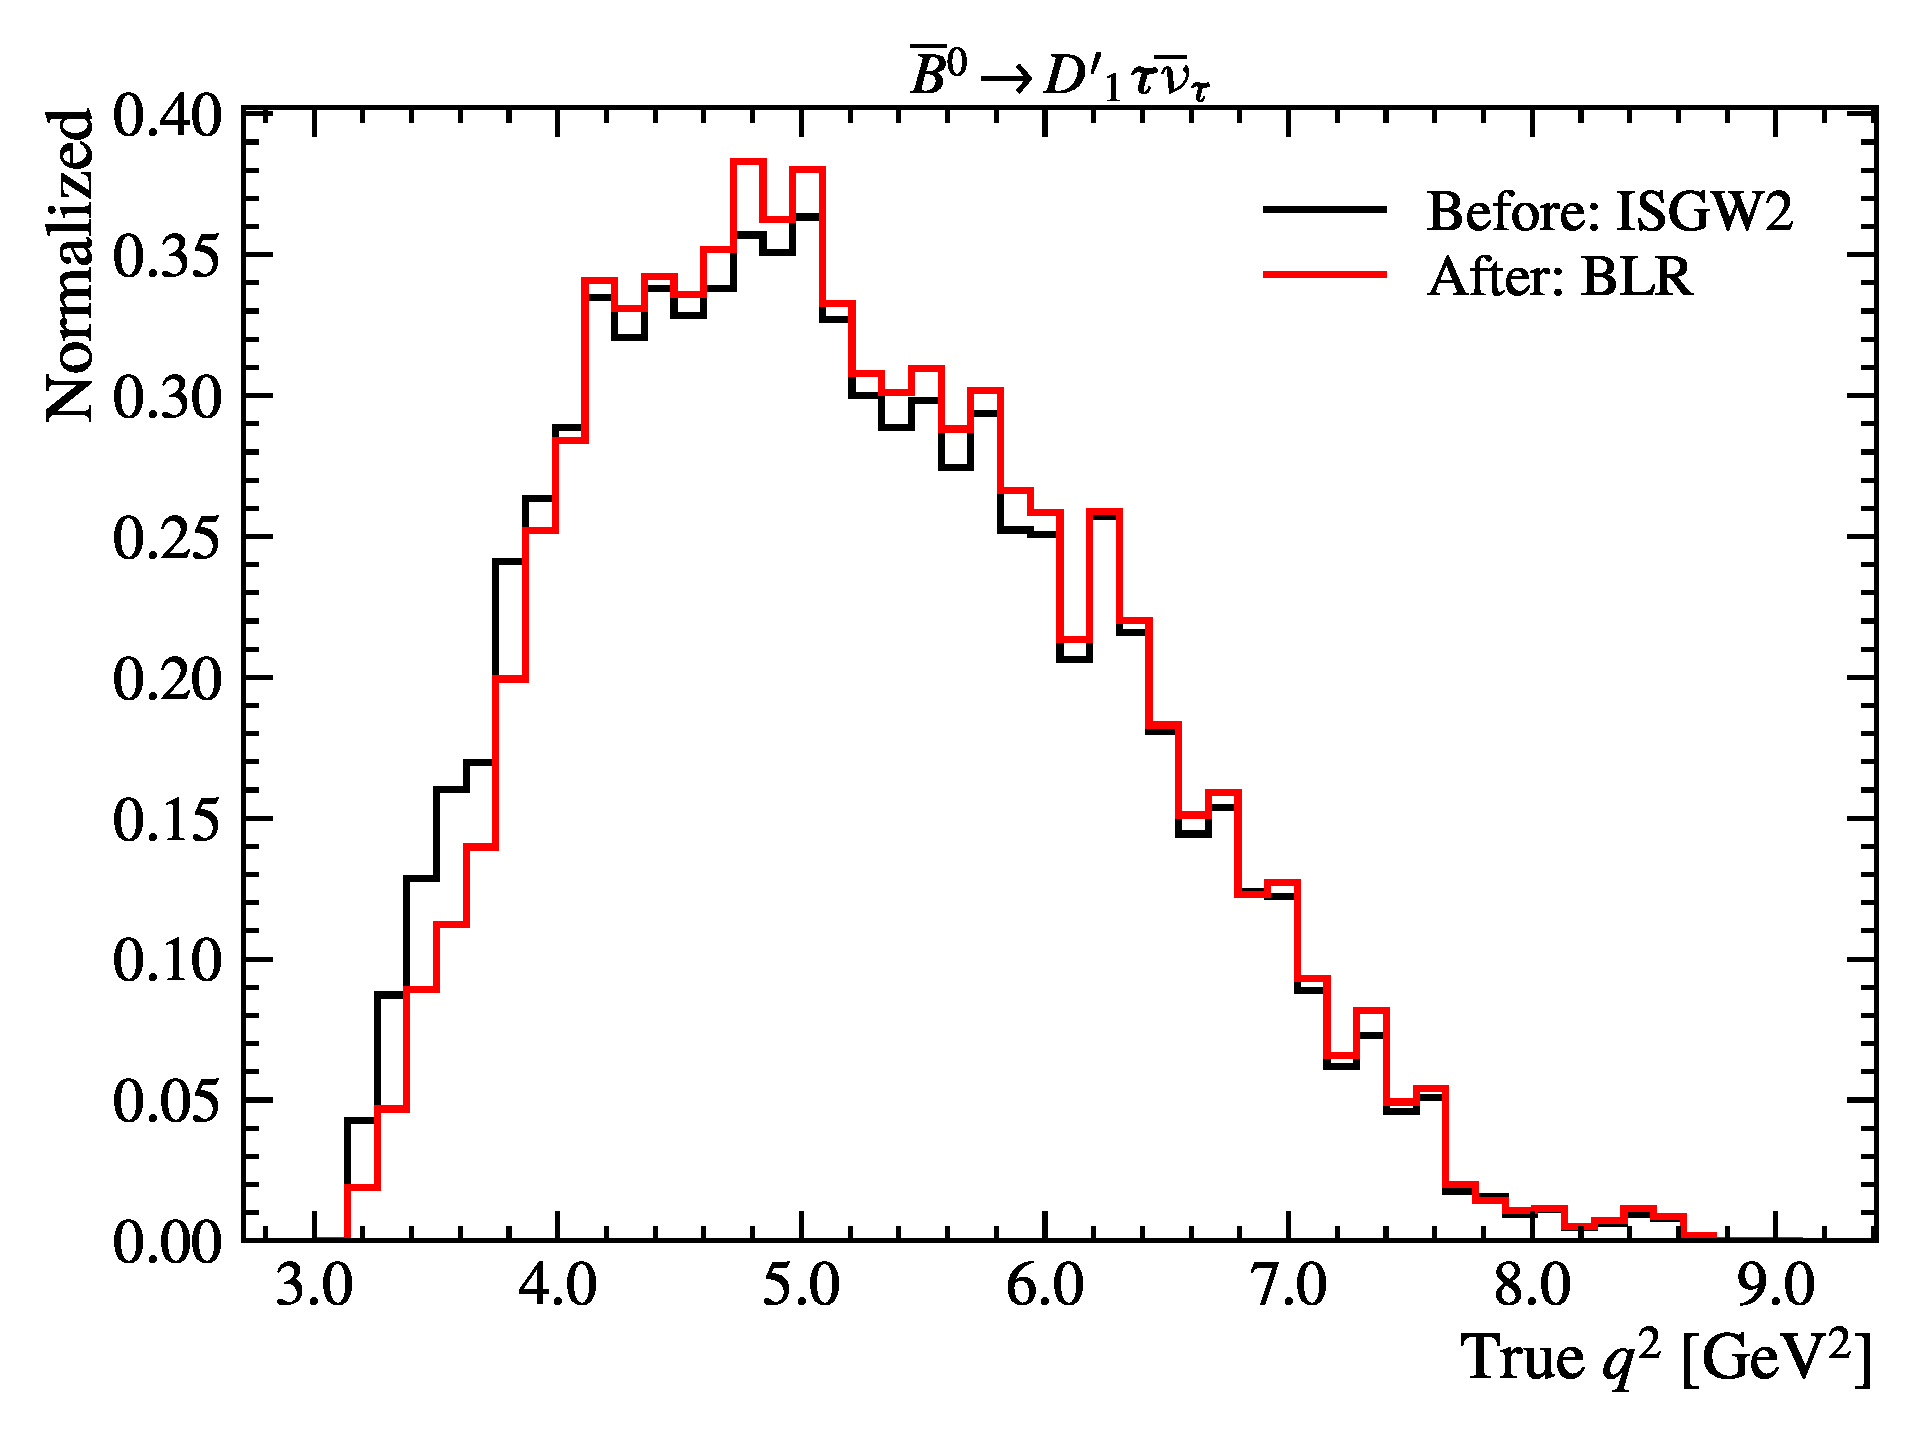
\includegraphics[width=0.24\textwidth]{
        ./figs-mc-correction/reweighting-form-factors/DststTau/D1pststTau.pdf
    }

    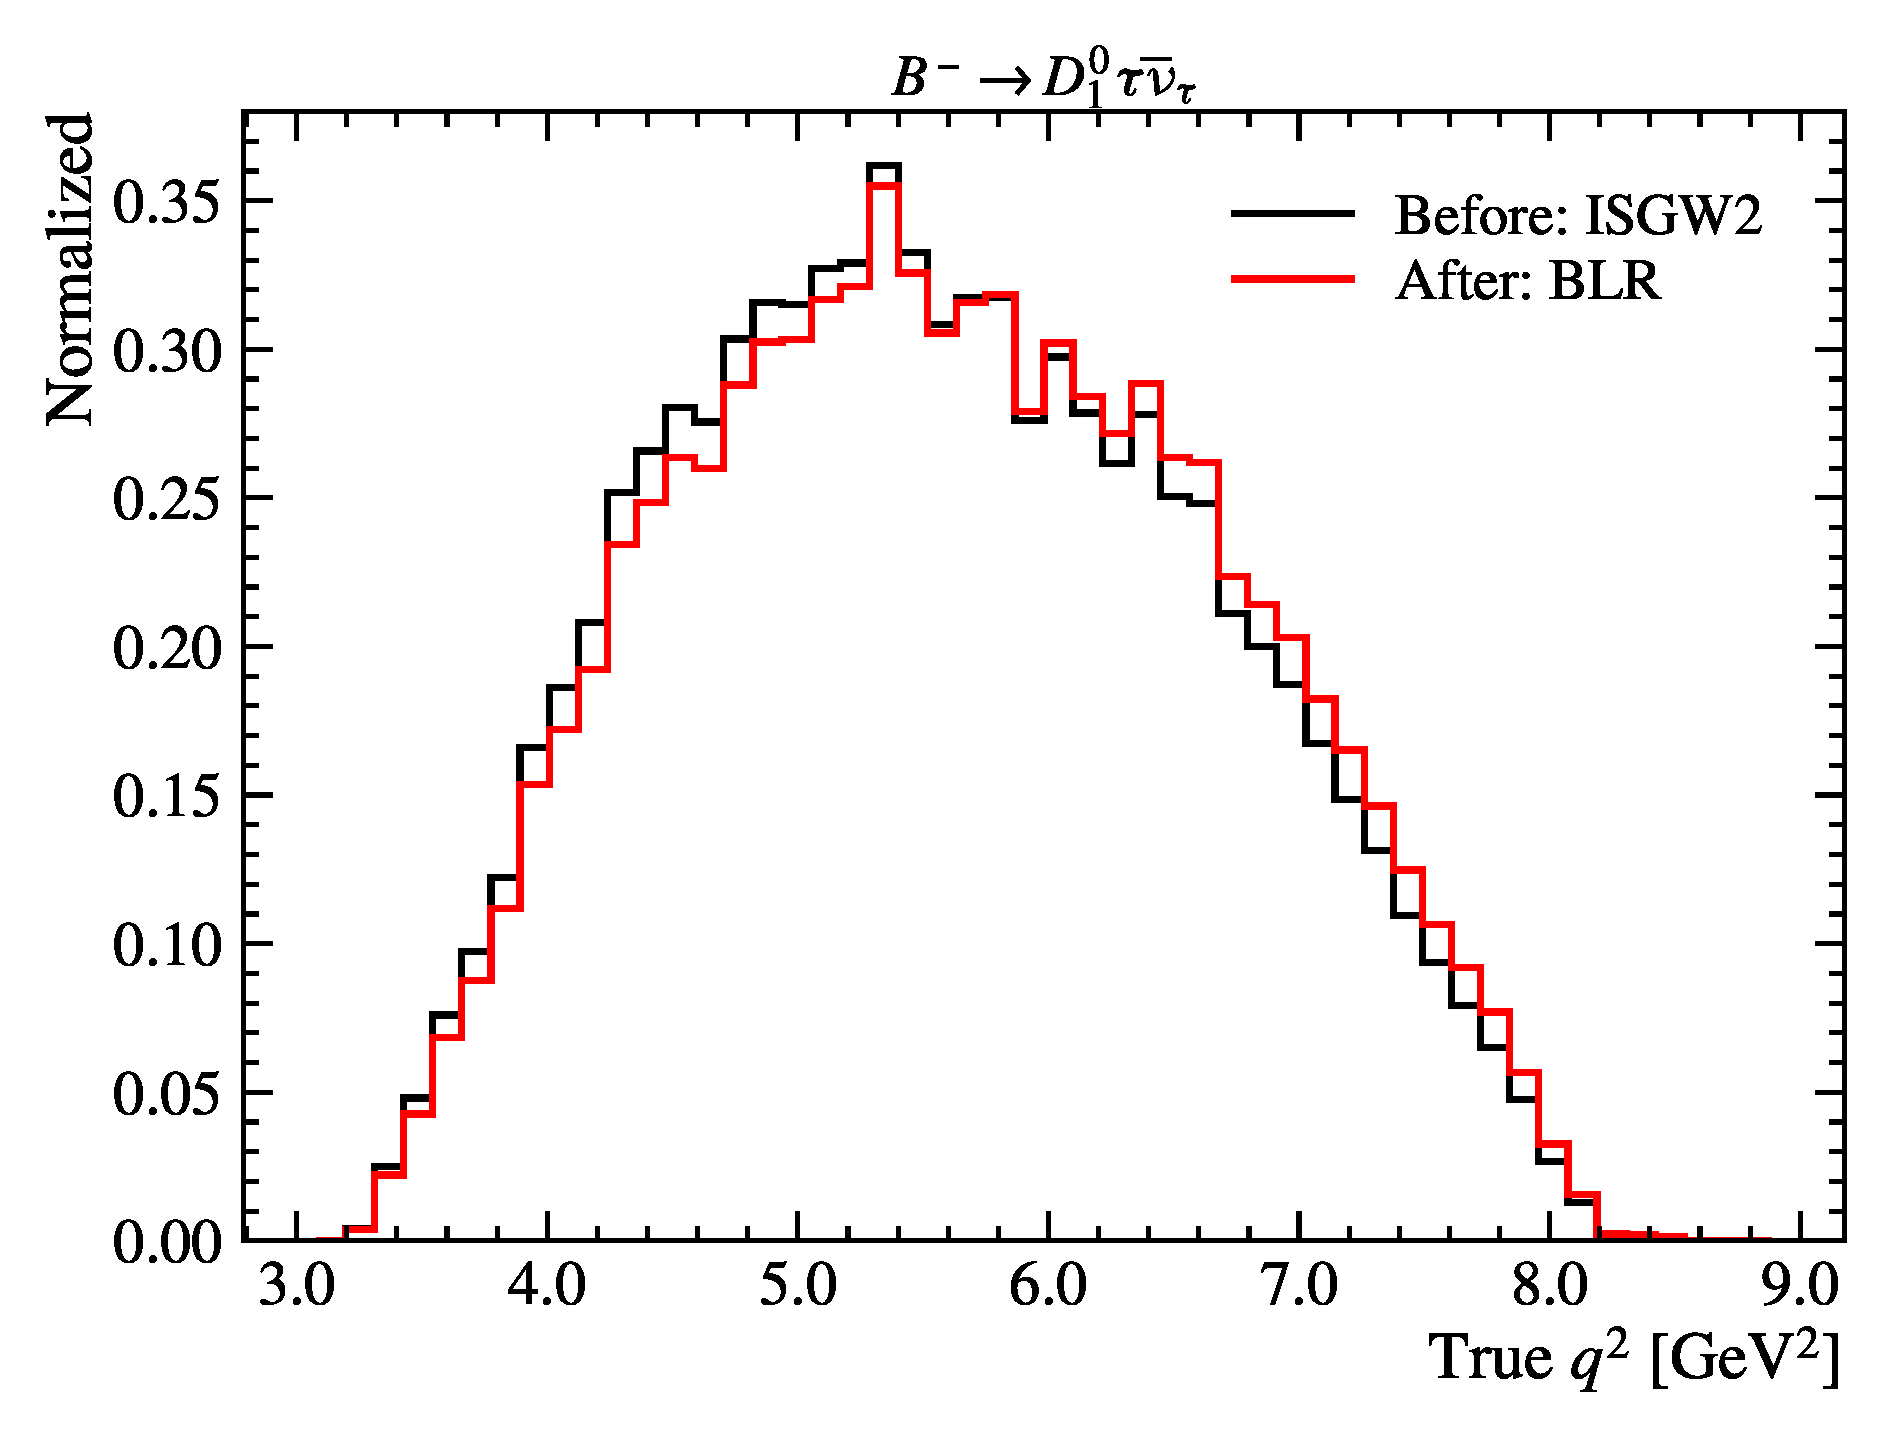
\includegraphics[width=0.24\textwidth]{
        ./figs-mc-correction/reweighting-form-factors/DststTau/D1stst0Tau.pdf
    }
    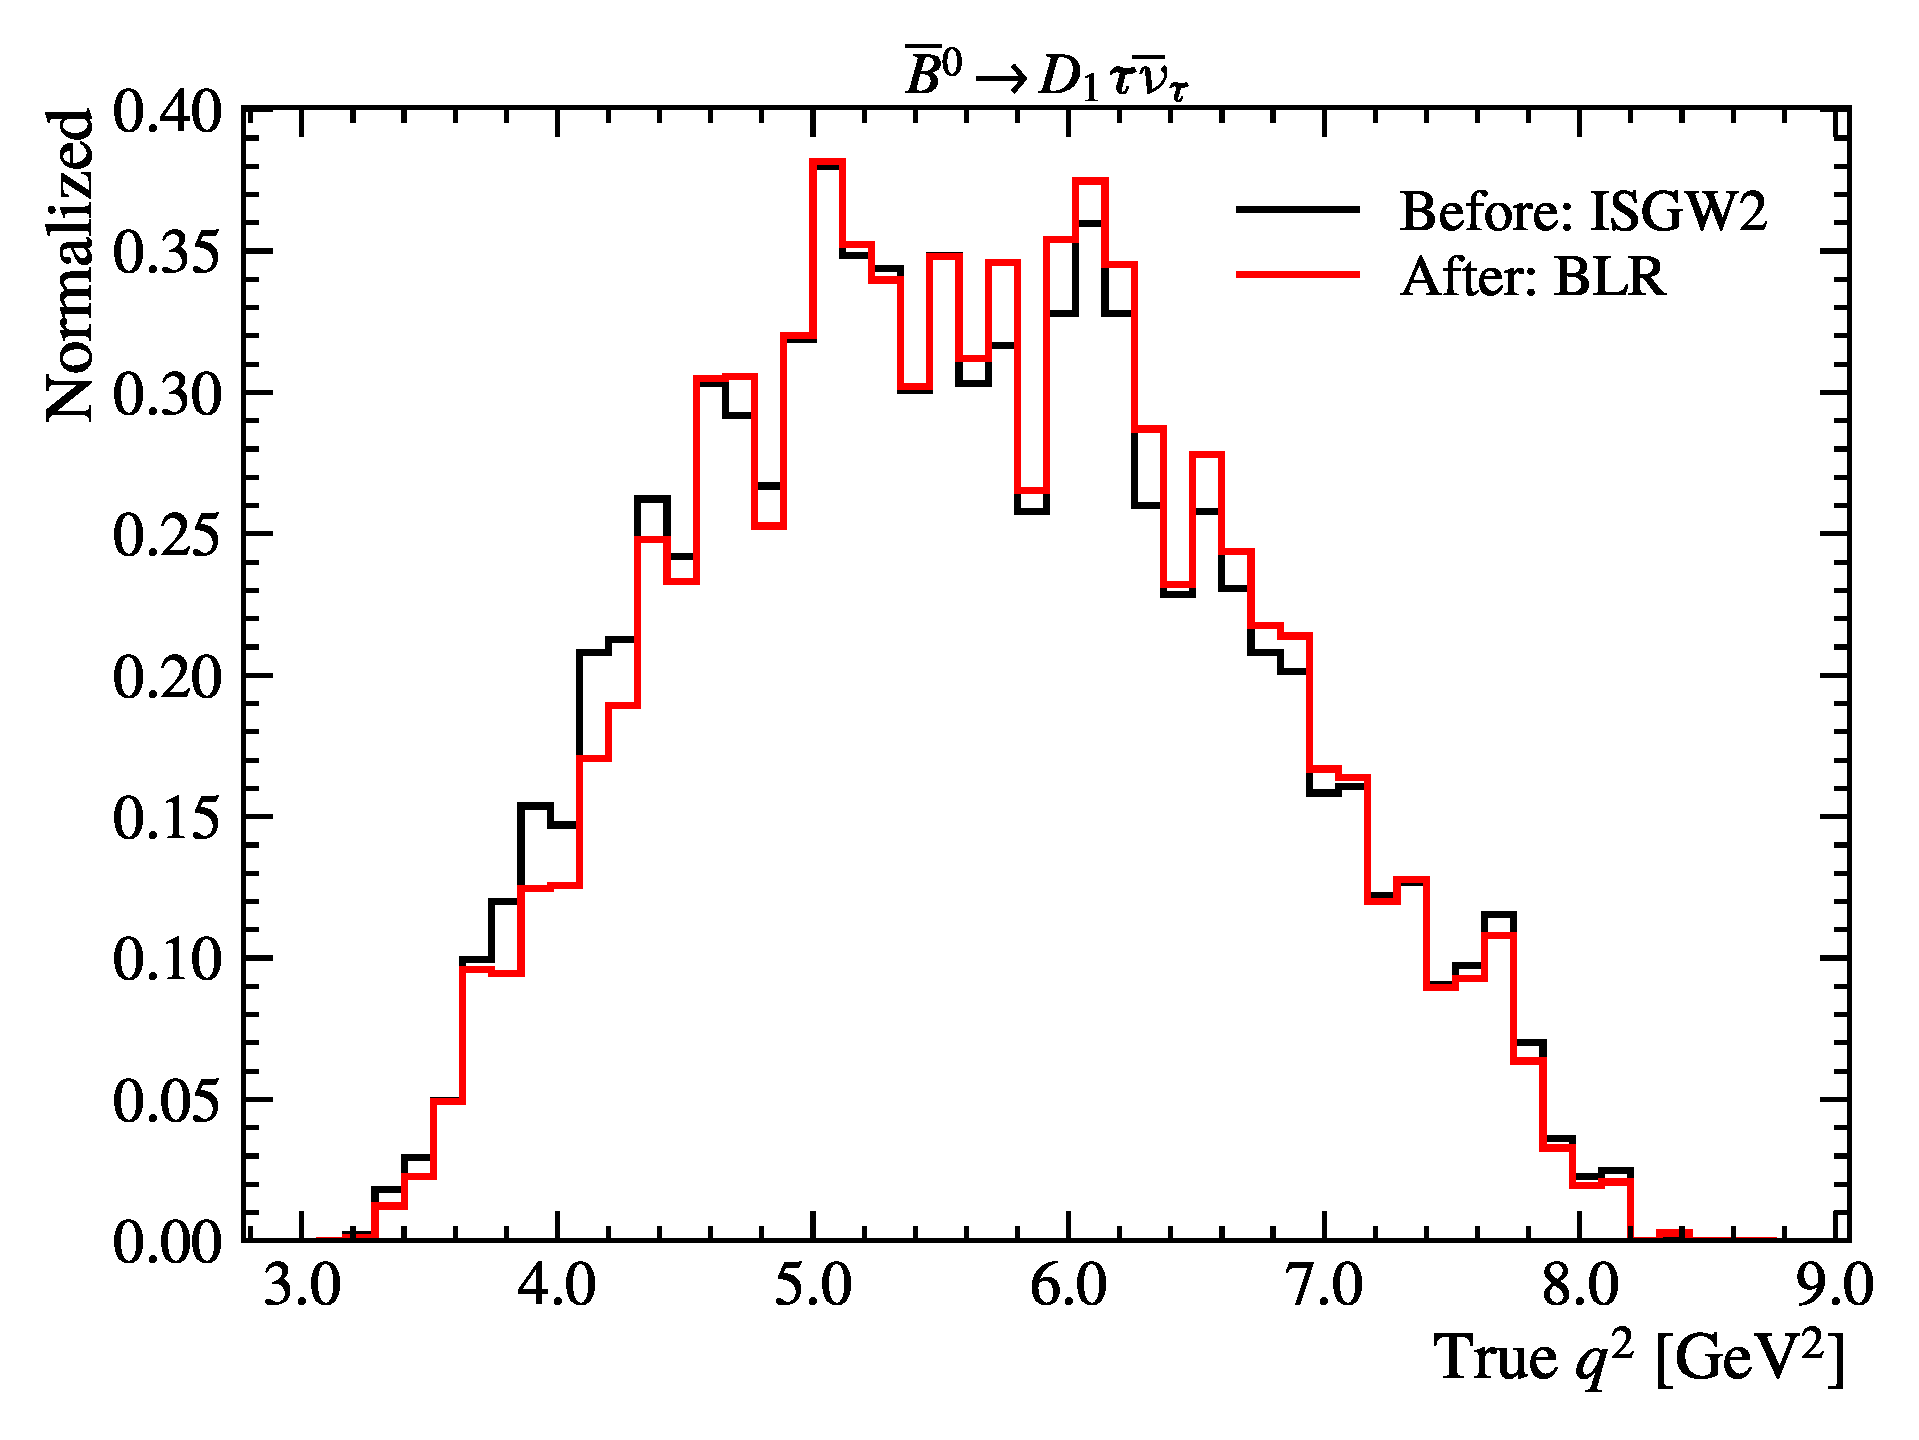
\includegraphics[width=0.24\textwidth]{
        ./figs-mc-correction/reweighting-form-factors/DststTau/D1ststTau.pdf
    }
    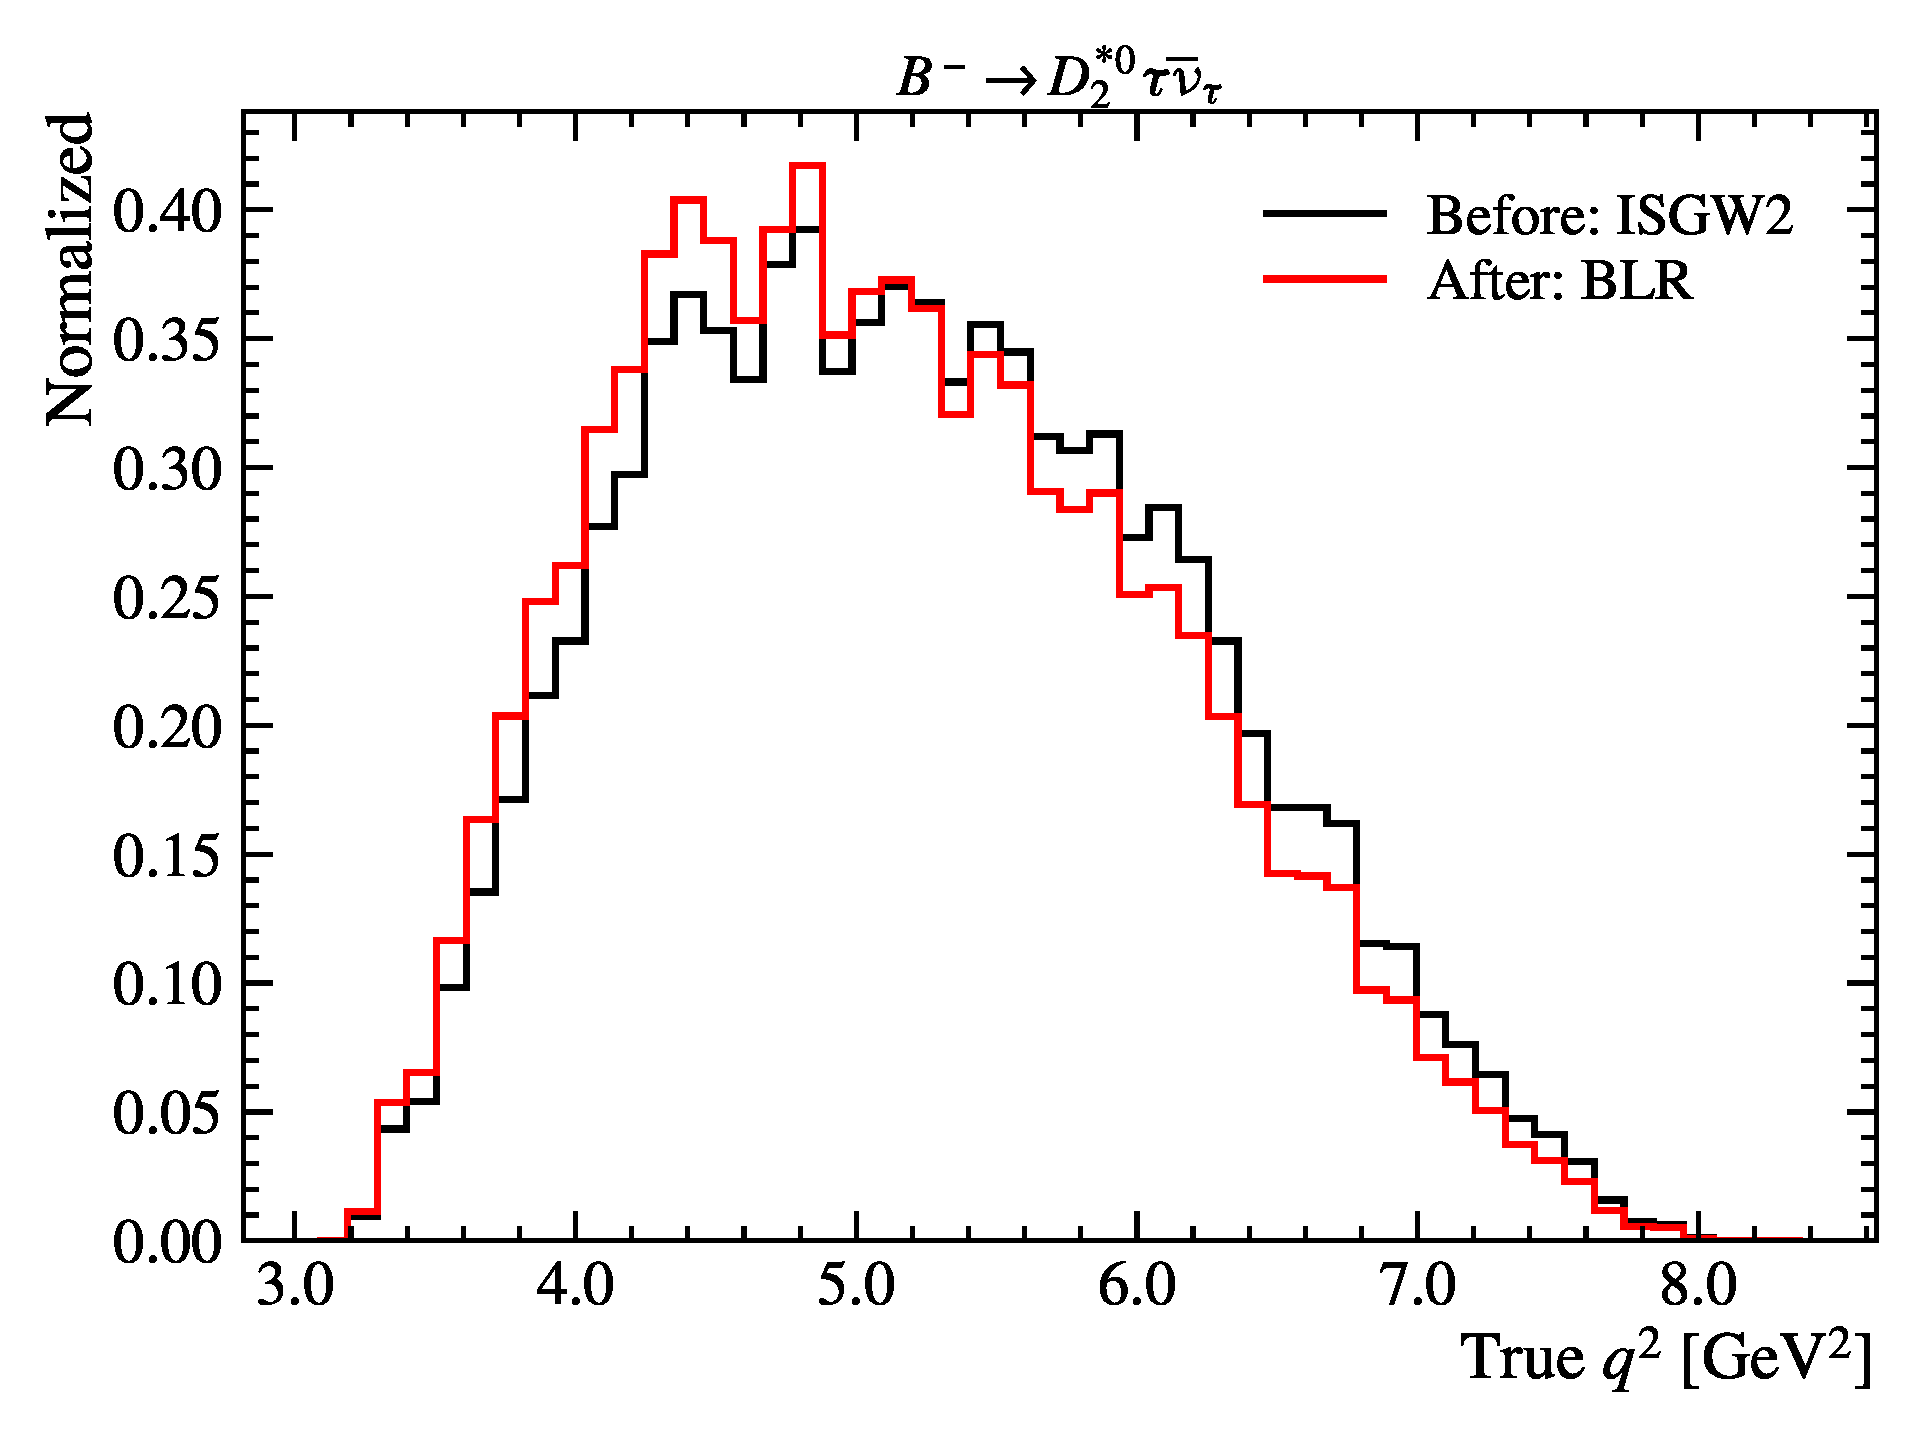
\includegraphics[width=0.24\textwidth]{
        ./figs-mc-correction/reweighting-form-factors/DststTau/D2stst0Tau.pdf
    }
    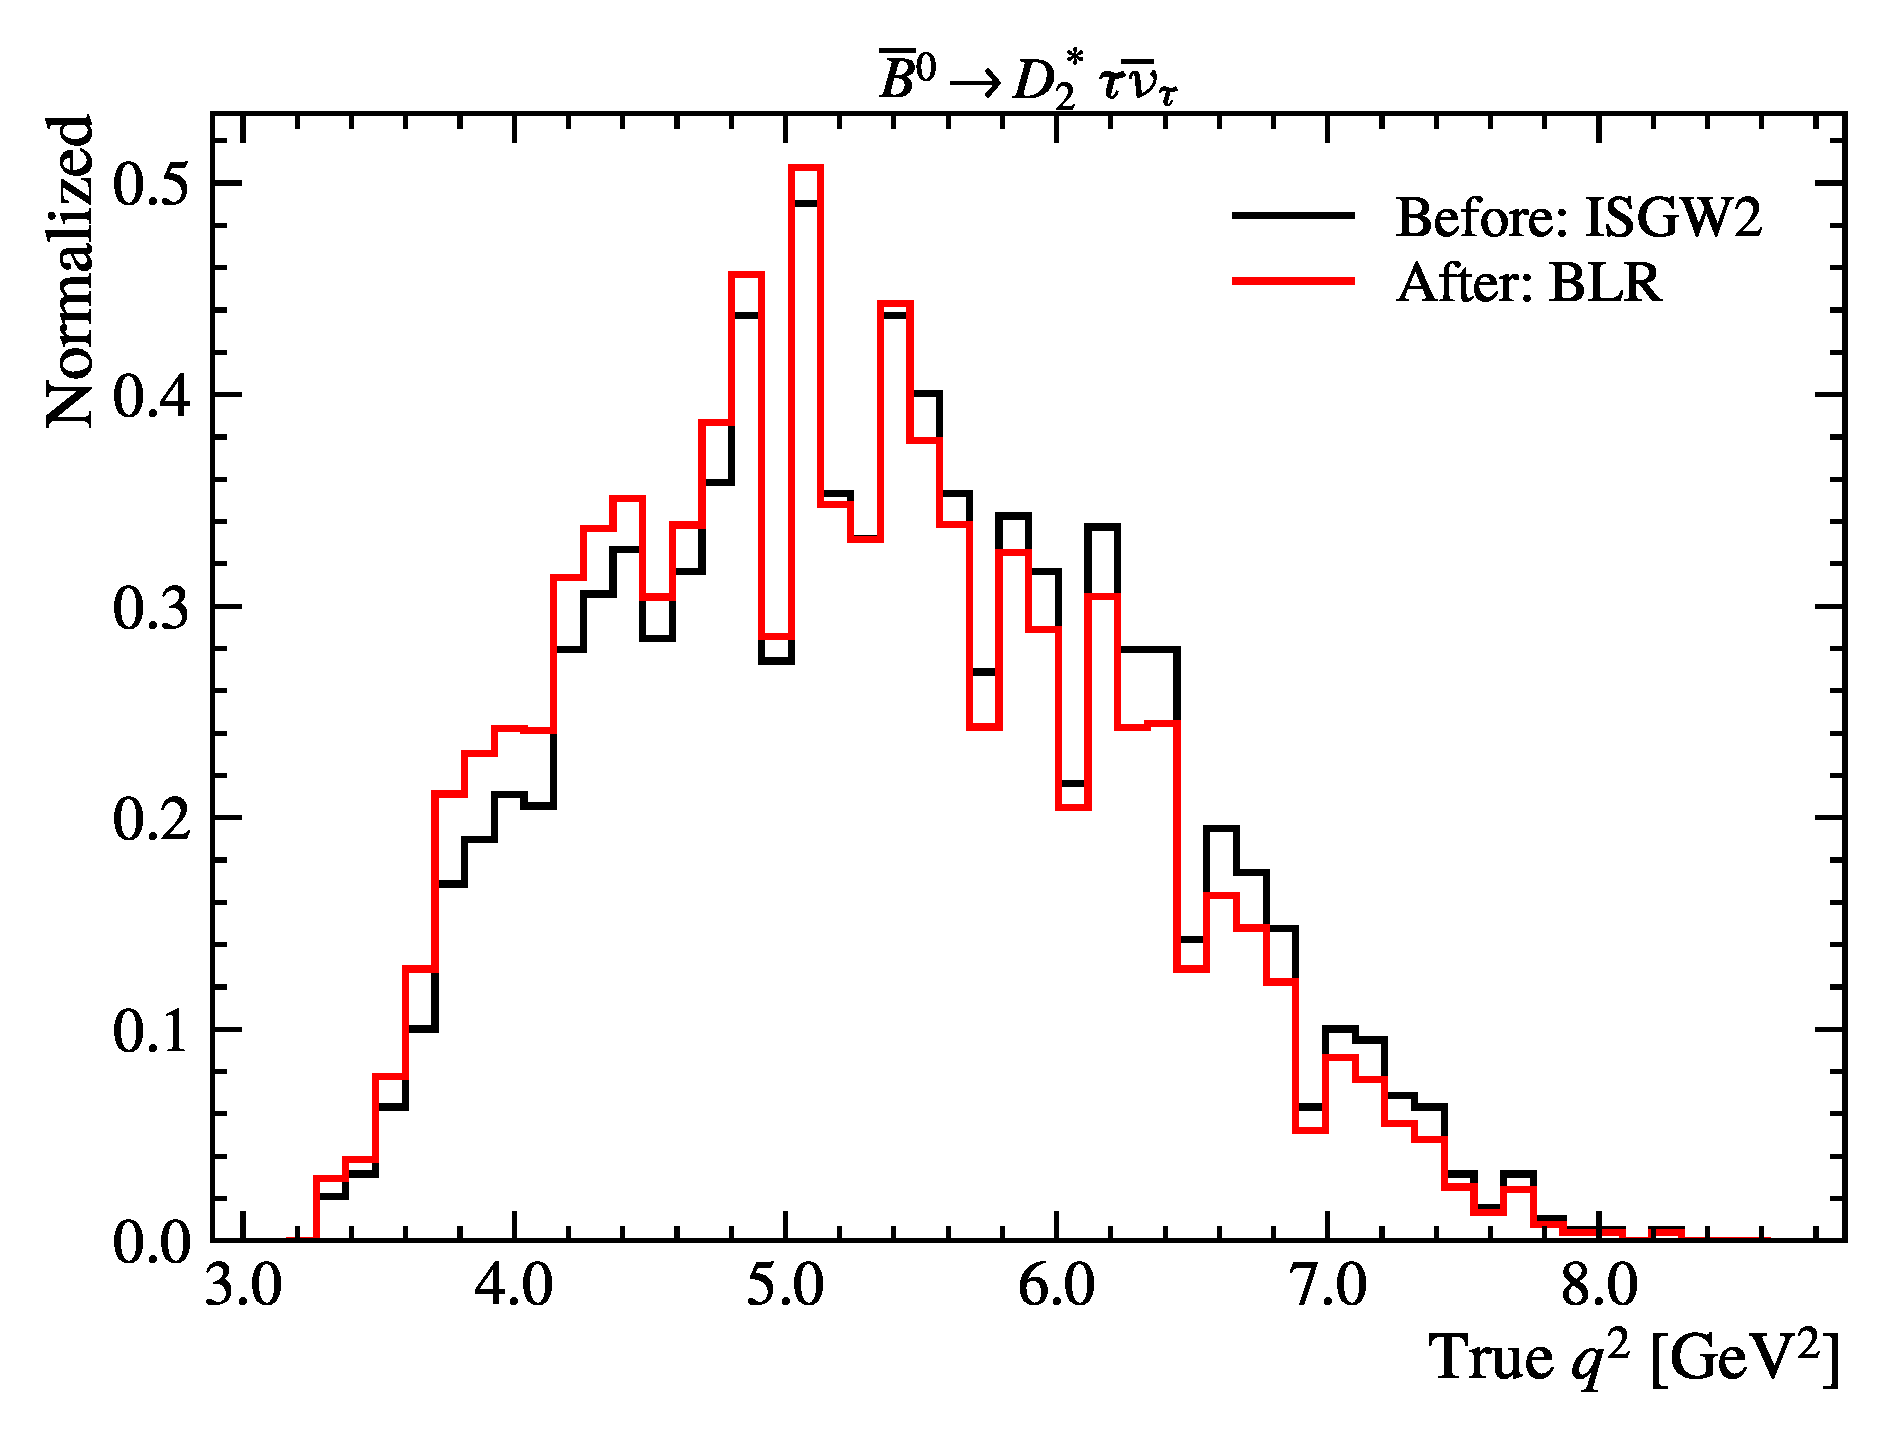
\includegraphics[width=0.24\textwidth]{
        ./figs-mc-correction/reweighting-form-factors/DststTau/D2ststTau.pdf
    }

    \caption{
        Form factor reweight effect on $D^{**}\tau$ MC templates.
        Parameters are shifted based an initial fit.
    }
    \label{fig:ff-rwt-Dstst-sig-like}
\end{figure}


\subsection{Tracking efficiency}

The track reconstruction efficiencies,
defined as $\frac{N_\text{reconstructed}}{N_\text{reconstructable}}$ for
\emph{long tracks}\footnote{
    Long tracks means that the tracks have hits recorded at both VELO (upstream)
    and T stations (downstream).
    They have the best tracking quality and most analyses use them exclusively.
},
are known to be different between data and MC.
The efficiencies are measured with a \emph{tag-and-probe} method on
\jpsi\mup\mun samples
which involves the following steps:
First, a long \muon-like track (tag) is and a partially reconstructed \muon-like
track (probe, non-long track) is required to form a \mun\mup vertex.
Then, the probe track is classified into two categories: The ones matched to a
long track, defined by sharing 70\% of hits with a long track in the T stations;
the ones \emph{not} matched.
Finally, a fit on the invariant mass of the \mun\mup vertex is performed to
extract number of signal events $N_\text{sig}$,
separately for matched and all probe tracks,
and the tracking efficiency is computed as:

\begin{equation}
    \epsilon_\text{tracking} \equiv
        \frac{N_\text{reconstructed}}{N_\text{reconstructable}}
        = \frac{N_\text{sig,matched}}{N_\text{sig,all}}
\end{equation}
For more information, refer to \cite{LHCb-PUB-2011-025,LHCb-DP-2013-002}.

To correct for the tracking discrepancy between data and MC,
the efficiency ratios\footnote{
    The efficiency ratios are taken from
    \techurllink{https://twiki.cern.ch/twiki/bin/viewauth/LHCbInternal/LHCbTrackingEfficiencies}{
        twiki/internal/LHCbTrackingEfficiencies}.
}
($\frac{\epsilon_\text{data}}{\epsilon_\text{MC}}$),
binned in $\eta$ and \ptot of the track,
between data and MC are provided by the \trackcalib package.
The correction is applied as a weight on a per-event basis.
The efficiency ratio table is shown in \cref{fig:trackcalib-eff}.

% Taken from RD+'s ANA
\begin{figure}[htb]
    \centering
    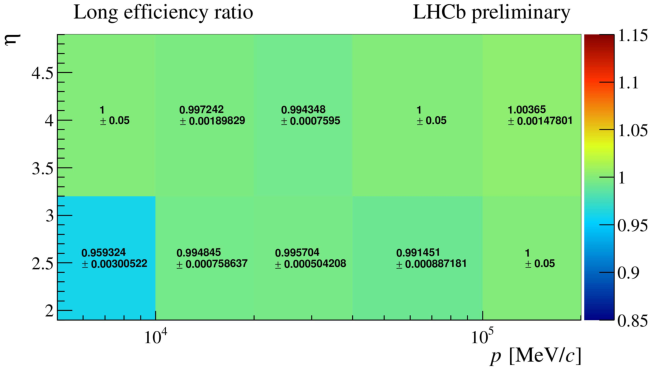
\includegraphics[width=0.6\textwidth]{./figs-mc-correction/reweighting-tracking/tracking_eff_2016.pdf}
    \caption{
        Tracking efficiency ratios
        $\frac{\epsilon_\text{data}}{\epsilon_\text{MC}}$.
        For 2016, only the table for the \emph{long} method is available.
    }
    \label{fig:trackcalib-eff}
\end{figure}

There are a few caveats: The efficiencies are available only for Sim09b MC
version, but in this analysis Sim09k is used.
The difference in simulation versions is ignored, given that this analysis
measures the \emph{ratio} of branching fractions, it is assumed that the
discrepancy would cancel in first order.
Additionally, the binning of \trackcalib efficiency ratio table,
shown in \cref{fig:trackcalib-slow-pi}, are more restricted than the selection
cuts.
Most notably in slow \pion, about 50\% of the tracks falls outside of the
binning range of the table for \Dstarp\mun MC decay mode.
To circumvent the problem, one method is to apply \trackcalib binning range cuts
on both data and MC, which leads to a significant loss in selection efficiency.
It is decided that in case a track falls outside of the binning range, the
efficiency ratio from its closest bin is applied.
It is hoped that additional discrepancy will be corrected in the
\emph{final reweighting} procedure.

% Generated in lhcb-ntuples-gen/studies/plot-RDX_spi_tracking_eff:
%   ./plot_spi_tracking.py
\begin{figure}[htb]
    \centering
    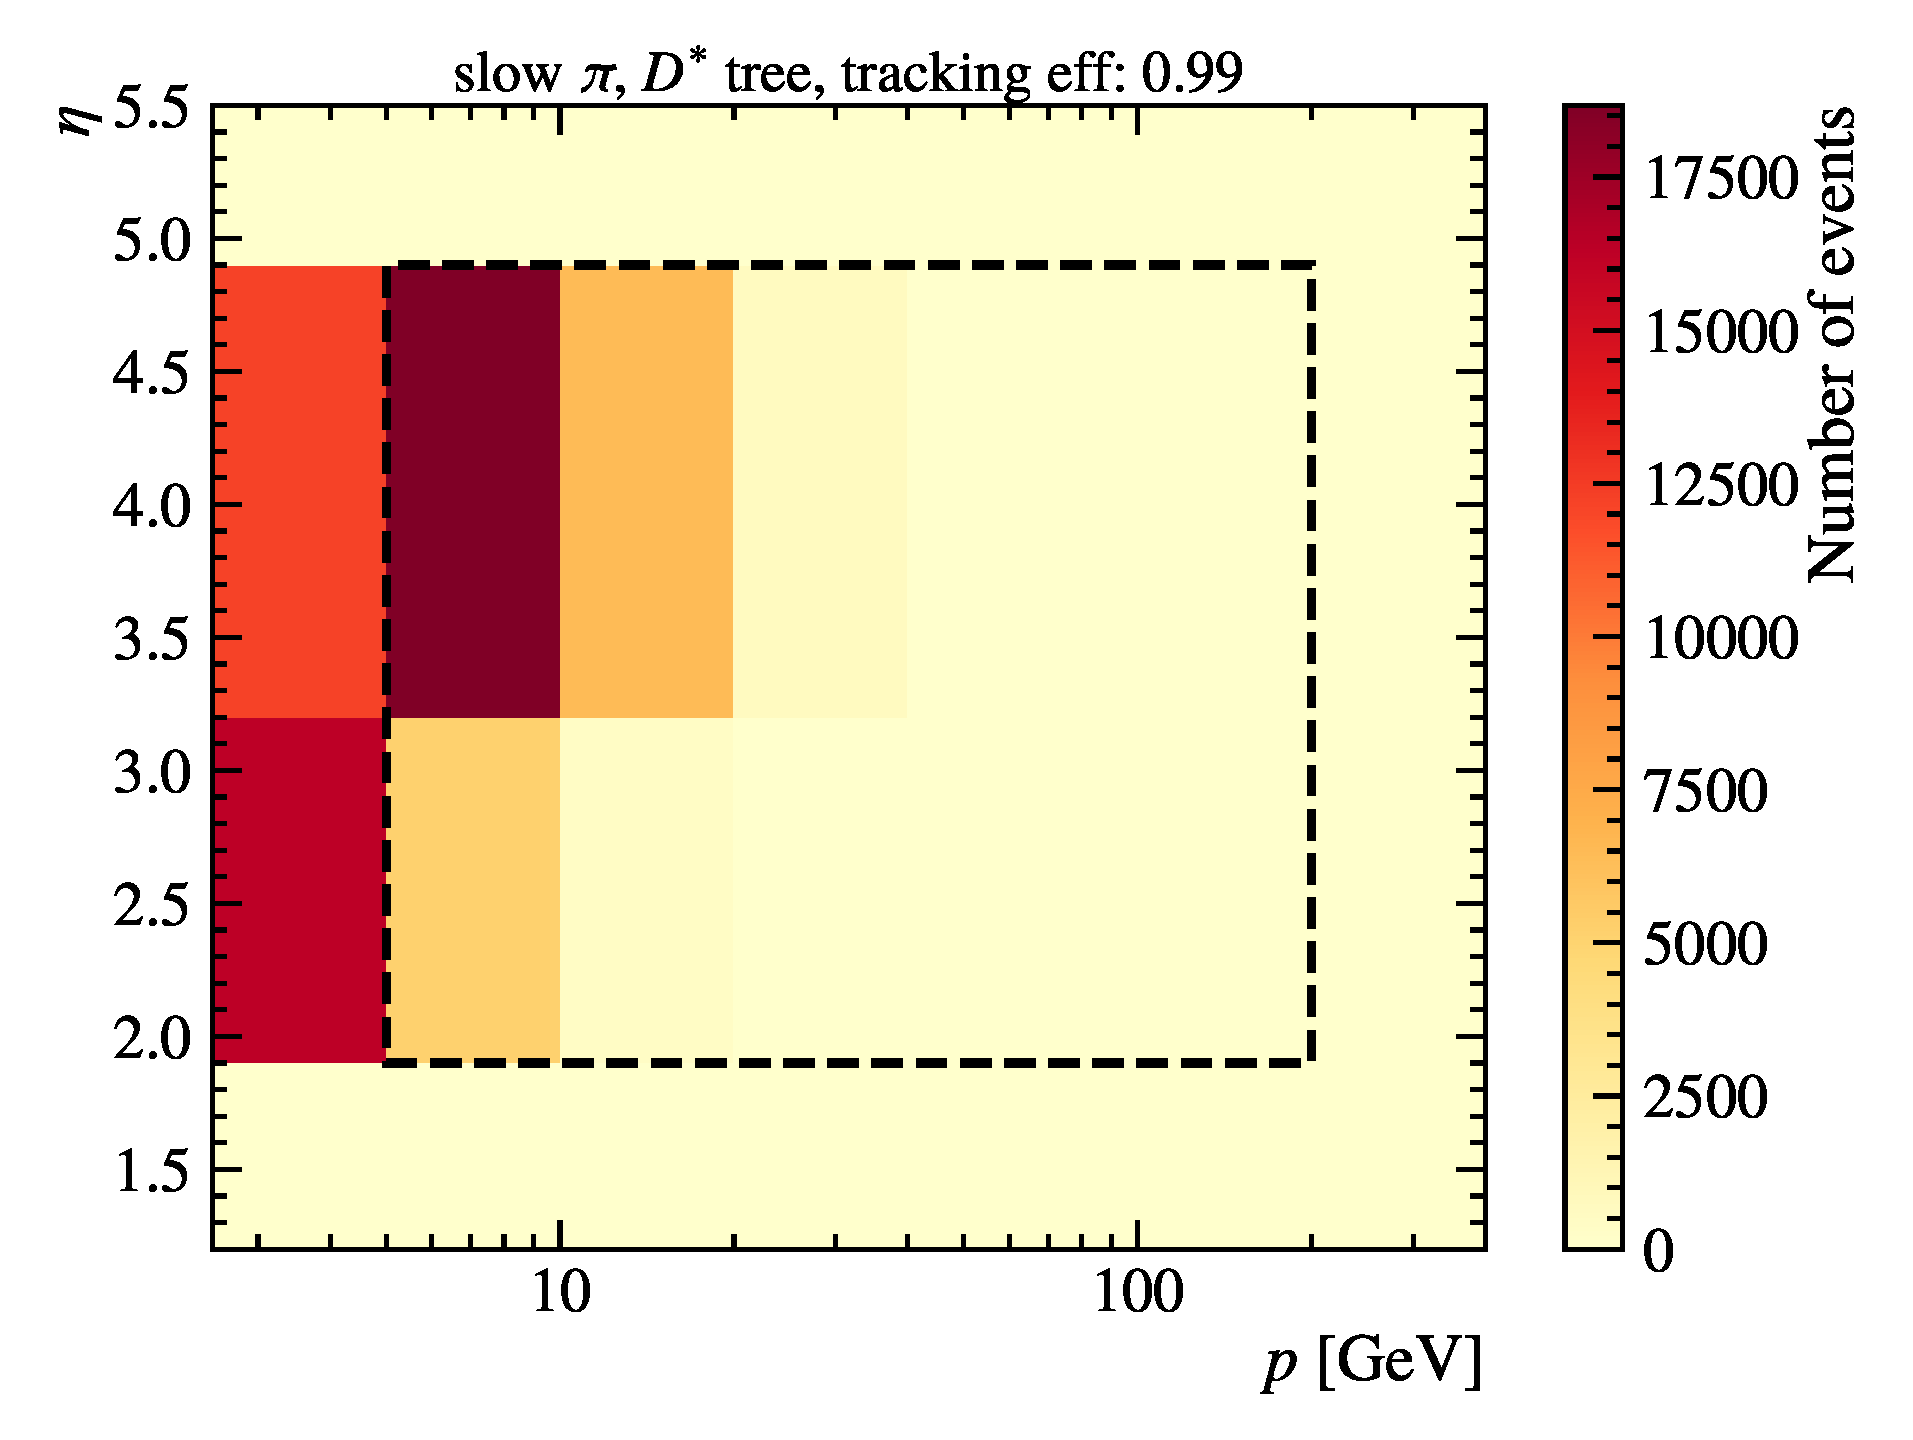
\includegraphics[width=0.7\textwidth]{./figs-mc-correction/reweighting-tracking/Dst_spi_p_eta.pdf}
    \caption{
        For slow \pion, about 50\% of tracks lies outside the binning region
        of the official \trackcalib binning range which is displayed by the
        dashed black box.
        The colored rectangles show number of events fall in each
        official \trackcalib bin.
        To avoid loss in selection efficiencies,
        correction ratios from nearby bin is applied.
        The study is done on $\Bzb \rightarrow \Dstarp \mun \neumb$ MC sample.
    }
    \label{fig:trackcalib-slow-pi}
\end{figure}


\subsection{$B$ kinematics and multiplicity}
\label{sec:data-mc:init-rwt:jpsi-k-correction}

Another known source of inconsistency between data and MC is the \B production
kinematics and multiplicity.
This is corrected by a separate set of
$\Bp \rightarrow \jpsi (\rightarrow \mun\mup) \Kp$
control samples, as described
in \cref{sec:reconstructed-samples:add-ctrl}, with both data and MC\footnote{
    In this case the MC is also \emph{stripped}, so the stripping line
    decisions exist.
}
sample filtered on the \smalltt{StrippingBetaSBu2JpsiKDetachedLine}.
Additional selections,
listed in \cref{tab:cut-jpsik},
are applied on the reconstructed sample, with PID
selections applied as weights (obtained from \pidcalib) for MC.
Tracking efficiency ratio corrections are also applied as weights
(obtained from \trackcalib) on MC samples.

An extended PID binning range is chosen to cover as much phase space of
\kaon and \muon as possible.
There may still be events outside the covering region, in which case the PID
weights from nearby bin is applied,
to avoid explicit cuts on the \jpsi\kaon data control sample.
The same strategy is applied on tracking weights.

\begin{table}[htb]
    \caption{Additional selections on $\jpsi K$ samples.}
    \label{tab:cut-jpsik}
    \centering
    \begin{tabular}{ c | rll}
        \toprule
        {\bf Particle}    & {\bf Variable}               & {\bf Cuts}               \\
        \midrule
        \kaon             & \pt                          & $> 500$ MeV              \\
                          & \PID{$K$}                    & $> 4$                    \\
        \midrule
        \mun, \mup        & \pt                          & $> 500$ MeV              \\
                          & \ipChiSq                     & $> 4$                    \\
                          & \PID{\muon}                  & $> 2$                    \\
        \midrule
        \mun\mup (\jpsi)  & $m_\text{mea}$\parnote{
            $m_\text{mea}$ refers to measured mass, which is the invariant
            mass given by the sum of daughters' four momenta,
            without any topological constraint.
            On the other hand, $m$ is given by a vertex fit,
            which is typically of better quality.
        }                                                & 3060--3140 MeV           \\
                          & \anyChiSq{FD}                & $> 25$                   \\
        \midrule
        \Bp               & $m$                          & 5150--5350 MeV           \\
                          & \anyChiSq{vertex}            & $< 18$                   \\
                          & \ipChiSq                     & $< 12$                   \\
                          & \DIRA                        & $> 0.9995$               \\
        \bottomrule
    \end{tabular}
    \begin{flushleft}
        \parnotes
    \end{flushleft}
\end{table}

A \sPlot\ is then performed on $J/\psi K$ data control sample to subtract
the combinatorial background, which is shown in \cref{fig:fit-JpsiK-data}.
The fit models consists of a double Gaussian plus a Crystal bell for signal,
and an exponential background.

% Generated in /lhcb-ntuples-gen/run2-JpsiK, with:
%   make fit-2016
% need to install zfit, which can be done via:
%   pip install -r ./requirements.txt
% in the same folder. And for now this probably doesn't work on macOS
\begin{figure}[htb]
    \centering
    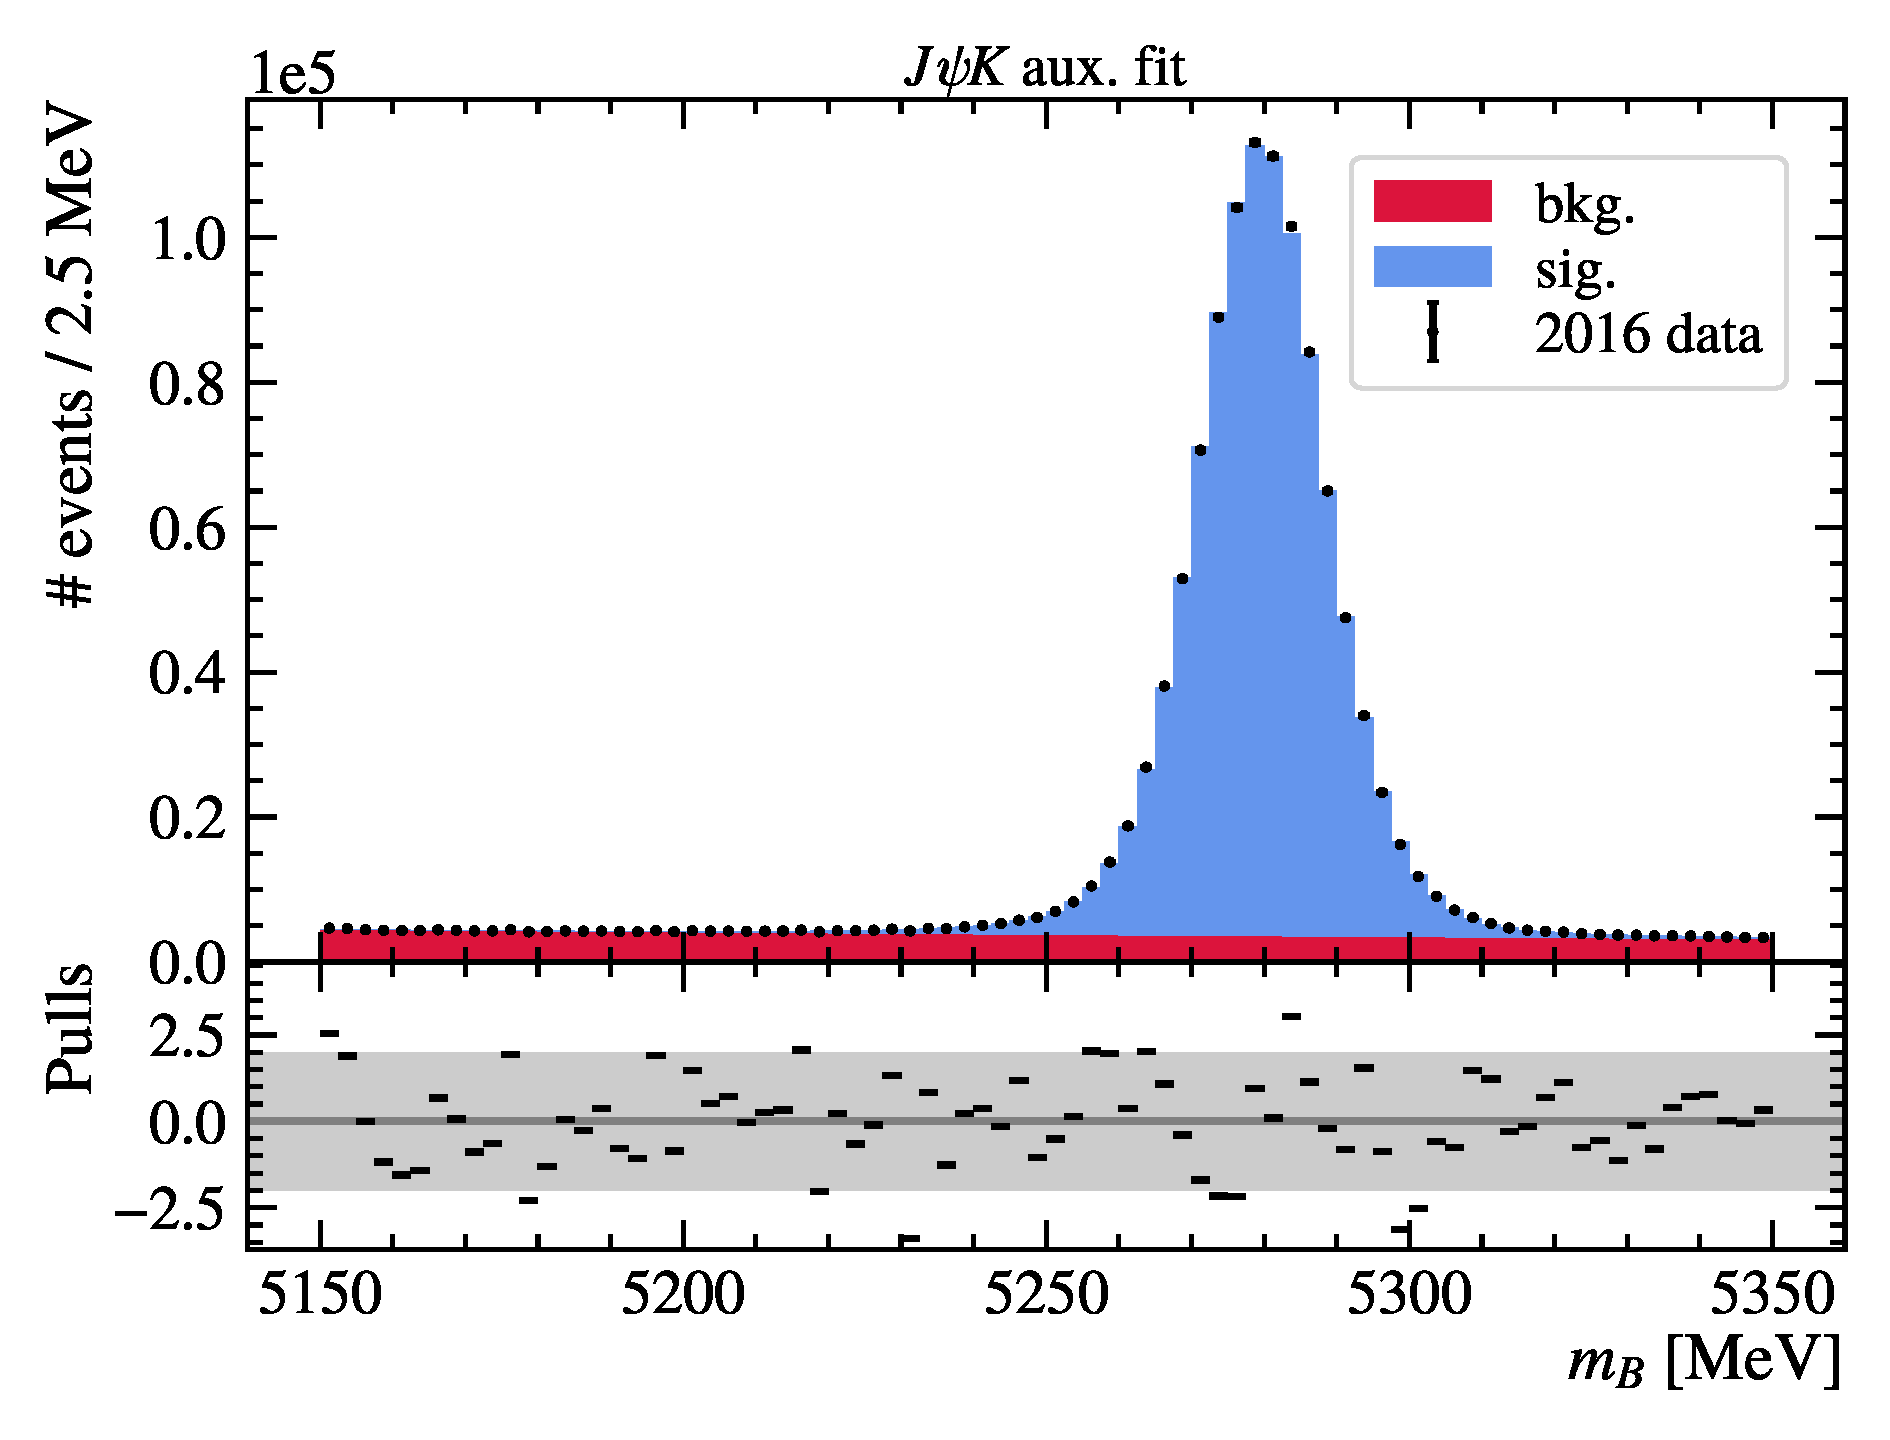
\includegraphics[width=0.45\textwidth]{./figs-mc-correction/reweighting-JpsiK/fit-JpsiK/fit_final.pdf}
    \hspace{1em}
    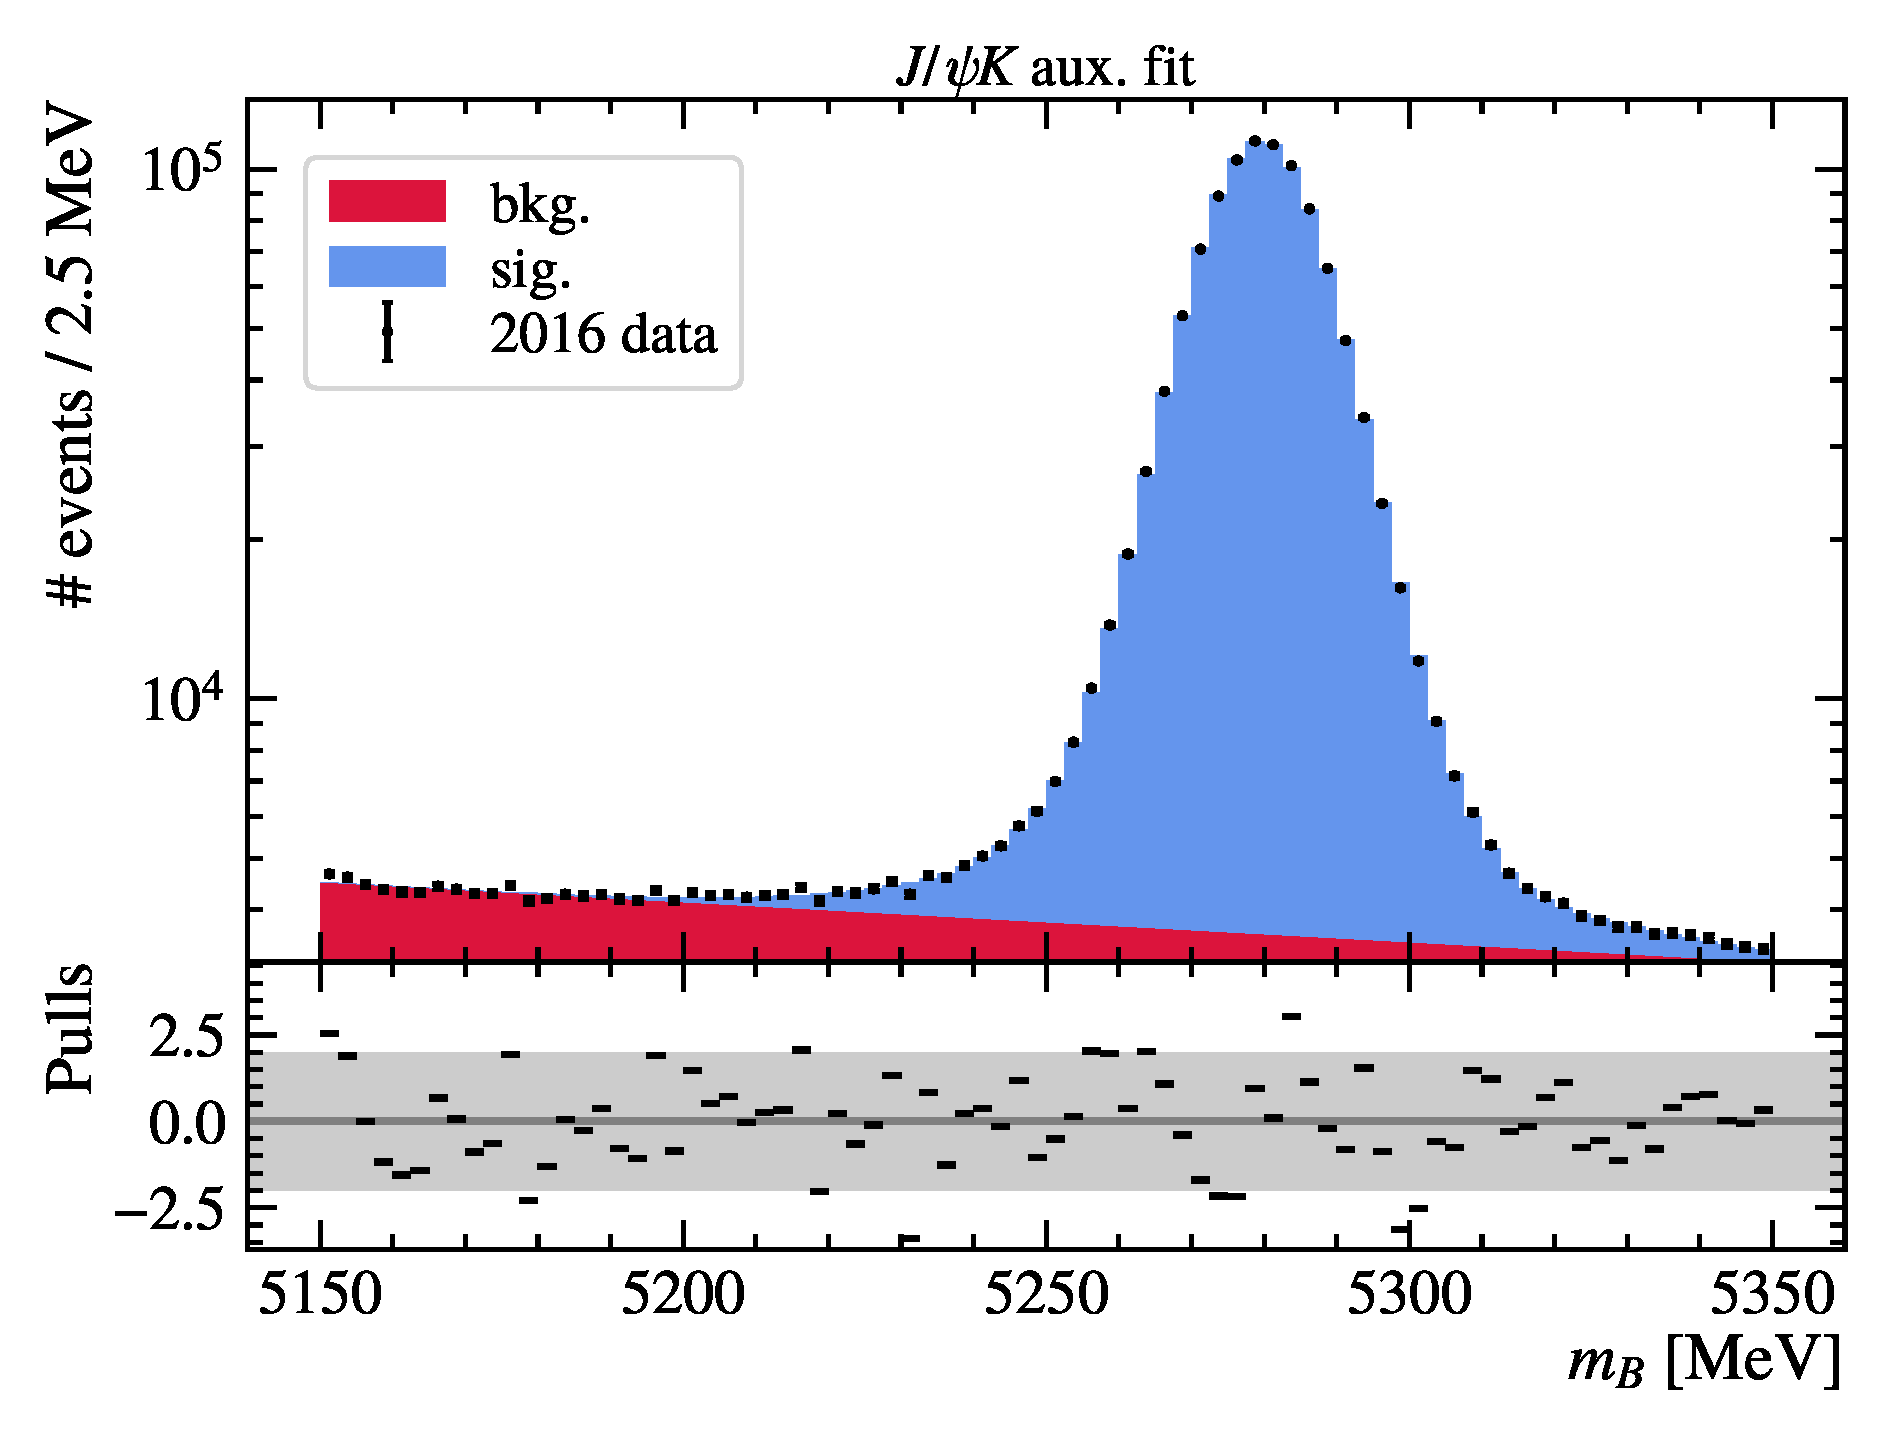
\includegraphics[width=0.45\textwidth]{./figs-mc-correction/reweighting-JpsiK/fit-JpsiK/fit_final_log_scale.pdf}

    \caption{
        Fit on $J/\psi K$ with a \sPlot procedure.
        The signal is modelled by a double Gaussian plus a Crystal bell;
        the background an exponential.
        Left and right show the same plot, with left having a linear $y$ axis,
        and right a log $y$ axis.
    }
    \label{fig:fit-JpsiK-data}
\end{figure}

A multi-stage\footnote{
    ``Multi-stage'' means that for reweighting stage $i$,
    all previous $i-1$ weights are applied.
} reweighting is performed on \sWeight-ed data and MC
(both are normalized, so the reweighting only corrects shape differences),
with stages defined in \cref{tab:rwt-JpsiK},
and the results shown in \cref{fig:rwt-JpsiK}.
The occupancy (nTracks) has to be corrected first,
because the PID efficiency weights depend this variable, and the weights alter
the shapes of the kinematic distributions of the \B decay daughters, which in
turn affect the \B kinematic distributions themselves.
The reweighting binning ranges are chosen such that:
\begin{itemize}
    \item They cover most of signal ranges of the data after applying \sWeight.
    \item The MC have enough population within these binning
        ranges so that there is no or few bins without a event.
\end{itemize}

When applying the \jpsi\kaon-derived weights to the nominal MC sample,
for events outside the binning regions,
the weights from nearby bins are applied.
This is to avoid introduce explicit kinematic cuts on the \B meson,
which is hard to apply consistently due to the fact that for
$B \rightarrow \jpsi\kaon$ decays,
there is no missing particle in the decay chain thus the \B momentum is
reconstructed in a more complete way,
whereas for $B \rightarrow D^{(*)} \lepton\neulb$, the missing neutrino(s)
makes the reconstructed \B momentum less precise.
It is assumed that the final reweighting is able to correct the remaining
differences in \B kinematics and occupancy.

\begin{table}[htb]
    \centering
    \caption{
        Reweighting stages and binning schemes for \B kinematic and
        occupancy reweighting.
    }
    \label{tab:rwt-JpsiK}
    \begin{tabular}{ c | c | c | c | c }
        \toprule
        {\bf Variable 1}    & {\bf Binning 1}      & {\bf Variable 2}   & {\bf Binning 2}    & {\bf Figure}   \\
        \midrule
        \B PV ndf           & 20, 1--250           & nTracks            & 20, 0--450         & \cref{fig:rwt-JpsiK:stage1} \\
        \B $\eta$           & 9, 2--6              & \B \pt             & 20, 0--30 GeV      & \cref{fig:rwt-JpsiK:stage2} \\
        \bottomrule
    \end{tabular}
\end{table}

% Generated in /lhcb-ntuples-gen/studies/plot-JpsiK_kinematic_reweighting
% by running:
%   plot_JpsiK_reweighting.py
% in the specified folder
\begin{figure}[htb]
    \begin{subfigure}{\textwidth}
        \centering
        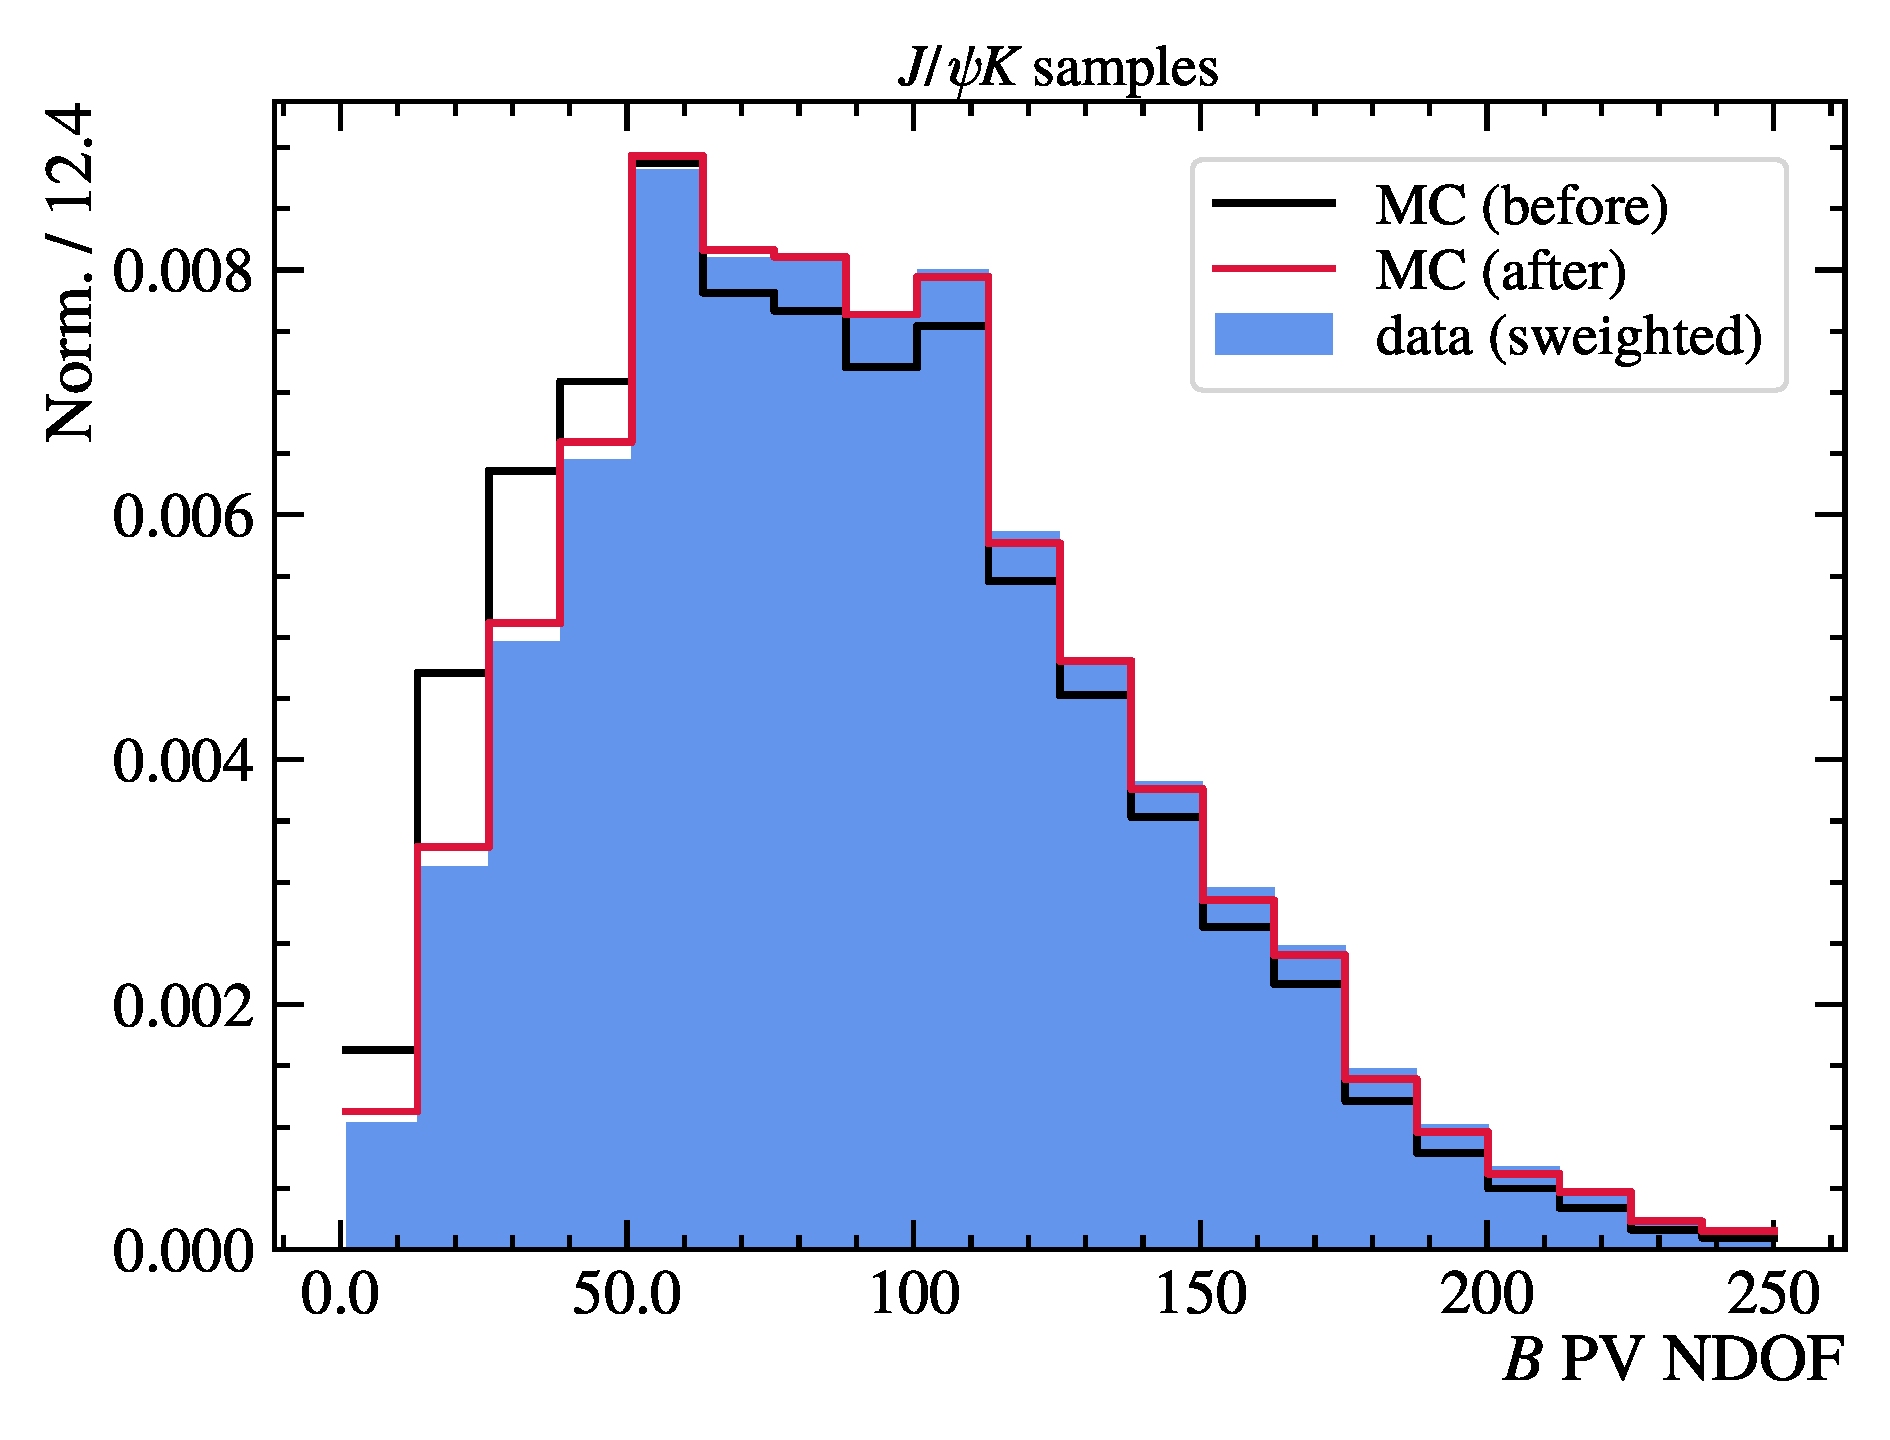
\includegraphics[width=0.45\textwidth]{./figs-mc-correction/reweighting-JpsiK/reweight-JpsiK/b_ownpv_ndof.pdf}
        \hspace{1em}
        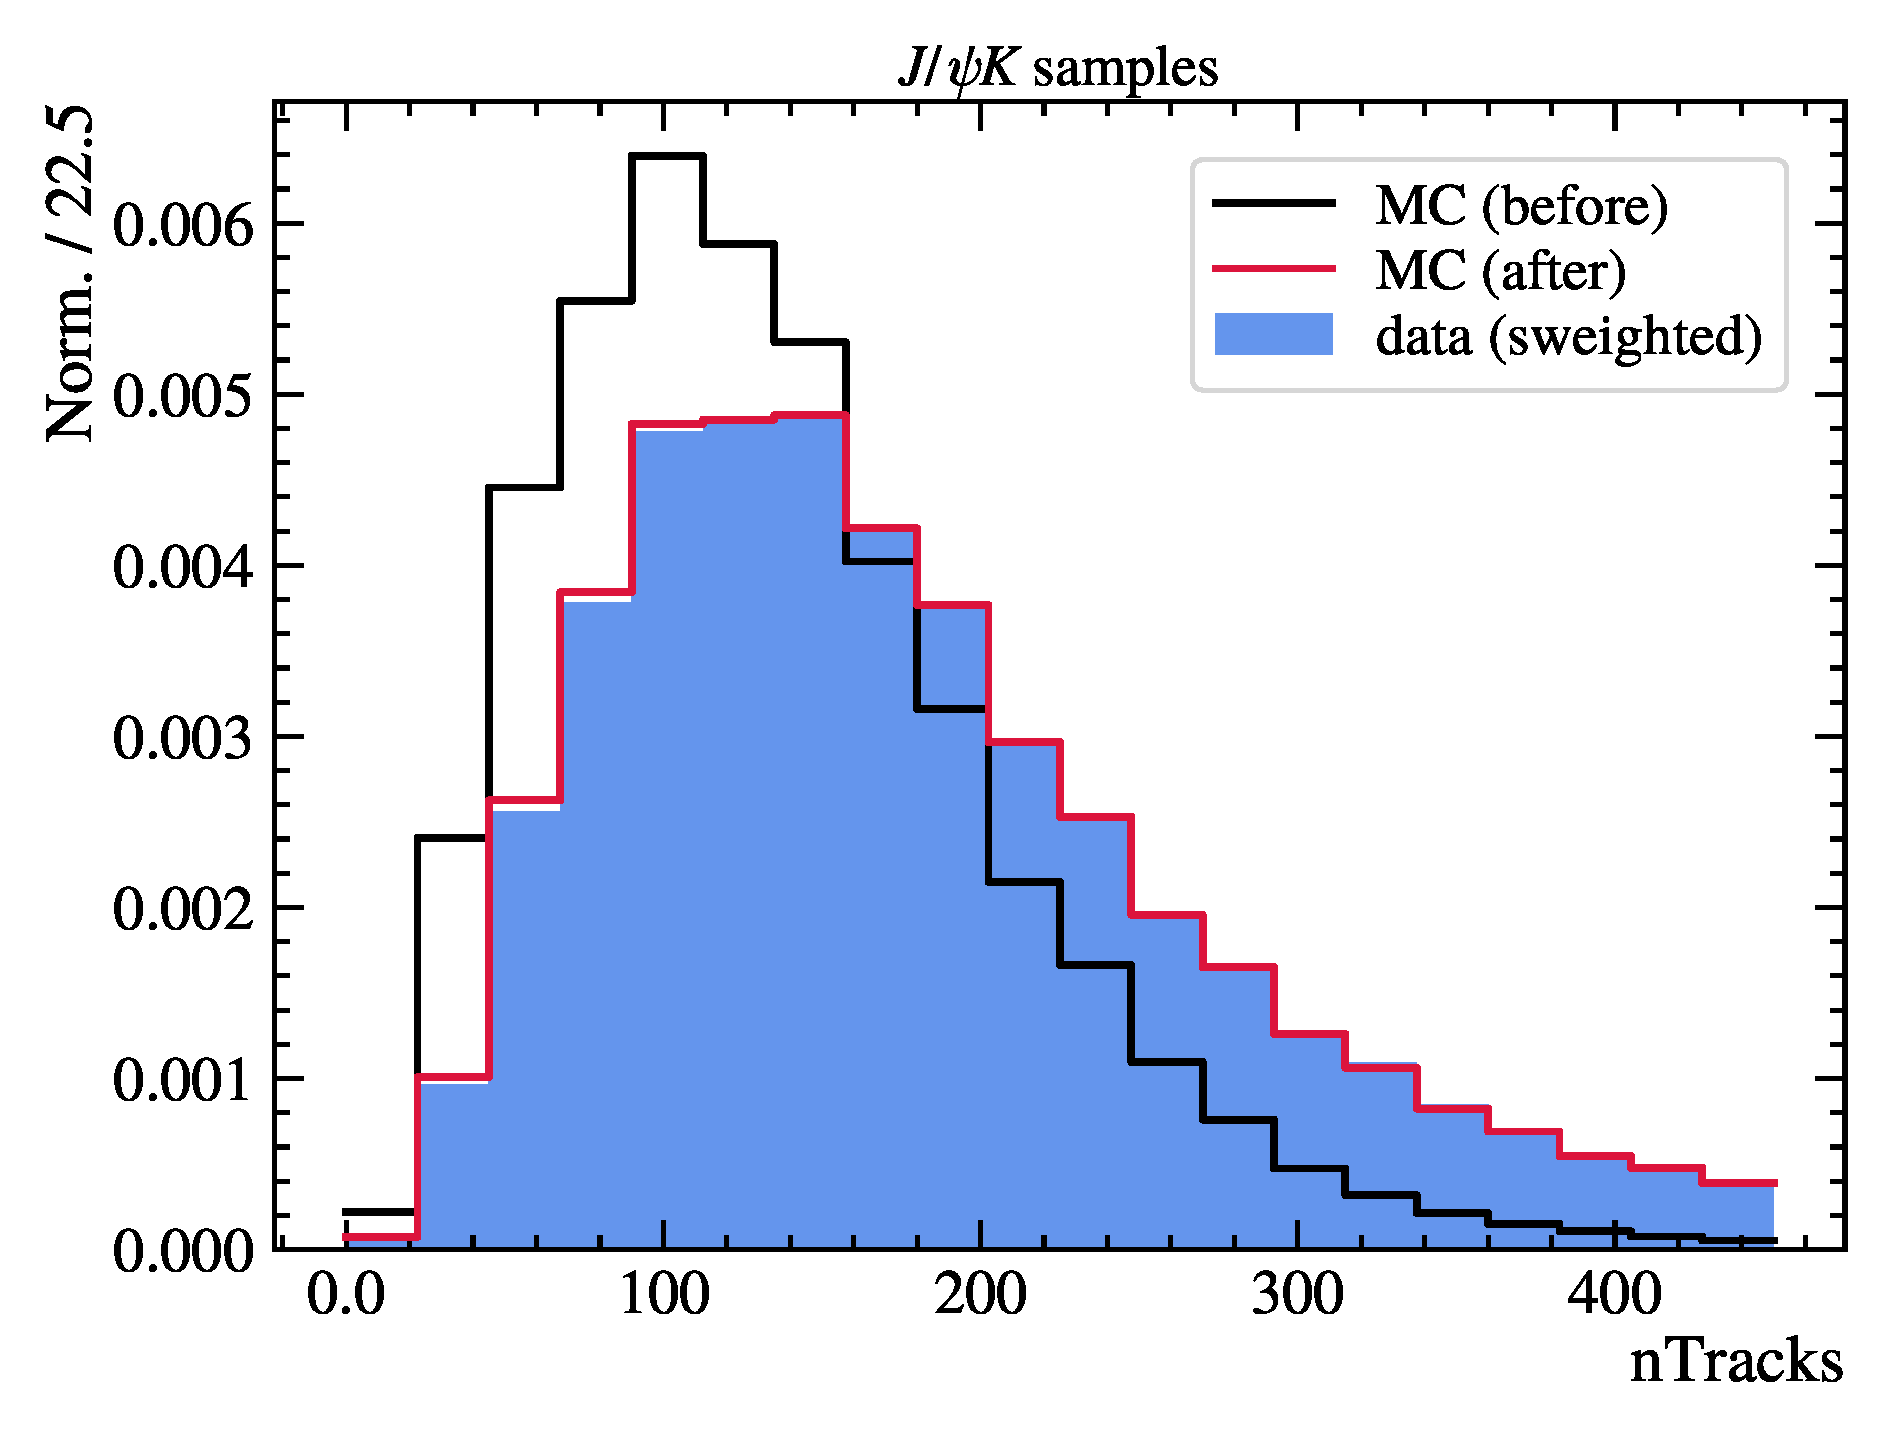
\includegraphics[width=0.45\textwidth]{./figs-mc-correction/reweighting-JpsiK/reweight-JpsiK/ntracks.pdf}
        \caption{Stage-1: $B$ PV ndf and nTracks.}
        \label{fig:rwt-JpsiK:stage1}
    \end{subfigure}

    \begin{subfigure}{\textwidth}
        \centering
        \includegraphics[width=0.45\textwidth]{./figs-mc-correction/reweighting-JpsiK/reweight-JpsiK/b_eta.pdf}
        \hspace{1em}
        \includegraphics[width=0.45\textwidth]{./figs-mc-correction/reweighting-JpsiK/reweight-JpsiK/b_pt.pdf}
        \caption{Stage-2: $B$ $\eta$ and $B$ \pt.}
        \label{fig:rwt-JpsiK:stage2}
    \end{subfigure}

    \caption{
        Effect of \B kinematic and occupancy reweighting,
        derived from \jpsi\kaon control samples.
        The ``MC (after)'' plots contain corrections from \emph{all stages}.
    }
    \label{fig:rwt-JpsiK}
\end{figure}


\section{Post-fit cocktail}
\label{sec:data-mc:postfit-cocktail}

Selected data samples are themselves cocktails because many
decay modes contribute to the $D^{(*)}\mu$ final state.
Therefore, meaningful comparisons between data and MC can only be performed
after a fit (termed \emph{initial fit}).

After the initial weights are applied to the fit templates,
a multi-step fit,
termed \emph{initial fit},
which is similar to the \emph{canonical} fit described in
\cref{sec:fit-to-data:fit-procedure},
with the sole exception that in the step-2 control fit,
the restriction (constraint on the log-likelihood)
on $D^{**}$ shape due to form factor uncertainties is enabled,
is performed with these templates to determine the yield and variations of
each template.
The fit results are displayed in
\cref{appx:suppl:init-fit-cocktail}.

Since the main objective of final reweighting is to correct the remaining
inconsistencies between data and MC due to detector responses,
it is important to reweight in a region where most discrepancies are induced by
such responses.
Therefore, a $\mmSq < 0.4$ GeV region,
dominated in normalization decay mode,
mostly free of effects due to fit modelling,
is used to derive the final weights.

A separate Python script\footnote{
    This can be fount at \techurllink{https://github.com/umd-lhcb/rdx-run2-analysis/blob/master/scripts/make_variated_histos.py}{
        github/umd-lhcb/rdx-run2-analysis
    }.
} is then used to build the post-fit cocktail with the following procedure:
\begin{enumerate}
    \item Apply the $\mmSq < 0.4$ GeV cut to obtain yields in the reweighting
        region based on fitted total yields.

    \item Some fit templates have variations which are specified by
        additionally provide variation templates at $\pm 1 \alpha$ and a
        interpolation/extrapolation method.
        This is described in \cref{sec:fit-to-data:fit-tmpl-vars}.

        The variation procedure is implemented in the Python script,
        and is checked against the variated templates extracted from the
        fitter output directly.
        For each template, the externally and internally variated ones differ
        bin-by-bin by less than $10^{-3}$.

    \item After effecting possible variations,
        each fit template is rescaled such that the scaled integral of the
        template matches the fitted yield.

    \item All MC templates are added together to form the
        \emph{post-fit cocktail}.
        The data-driven templates are subtracted from the \emph{data}
        template to form \emph{subtracted data} template
        which is comparable to the \emph{post-fit cocktail}.
\end{enumerate}


\section{Final reweighting}
\label{sec:data-mc:final-rwt}

The final reweighting is a multi-stage reweighting process by comparing
selected
kinematic and geometric variables of the \B decay daughters,
listed in \cref{tab:rwt-final-vars},
between \emph{post-fit cocktail} and \emph{subtracted data}
in the reweighting region, selected by a $\mmSq < 0.4$ GeV cut.
The reweighting is performed separately for \Dz and \Dstar channel;
the latter contains additional stages due to corrections to slow \pion.

The effects of final reweighting can be seen at
\cref{fig:final-rwt-d0} for \Dz channel, and
\cref{fig:final-rwt-dst} for \Dstar channel.

\begin{figure}[htb]
    \begin{subfigure}{\textwidth}
        \centering
        \includegraphics[width=0.32\textwidth]{./figs-mc-correction/reweighting-final/plot_step1-D0_iso-b_log_fd_chi2.pdf}
        \includegraphics[width=0.32\textwidth]{./figs-mc-correction/reweighting-final/plot_step1-D0_iso-d0_log_ip_chi2.pdf}
        \includegraphics[width=0.32\textwidth]{./figs-mc-correction/reweighting-final/plot_step1-D0_iso-mu_log_ip_chi2.pdf}
        \caption{Stage 1.}
    \end{subfigure}

    \begin{subfigure}{\textwidth}
        \centering
        \includegraphics[width=0.32\textwidth]{./figs-mc-correction/reweighting-final/plot_step2-D0_iso-k_comp.pdf}
        \includegraphics[width=0.32\textwidth]{./figs-mc-correction/reweighting-final/plot_step2-D0_iso-k_log_ip_chi2.pdf}
        \includegraphics[width=0.32\textwidth]{./figs-mc-correction/reweighting-final/plot_step2-D0_iso-k_pt.pdf}
        \caption{Stage 2.}
    \end{subfigure}

    \begin{subfigure}{\textwidth}
        \centering
        \includegraphics[width=0.32\textwidth]{./figs-mc-correction/reweighting-final/plot_step3-D0_iso-pi_comp.pdf}
        \includegraphics[width=0.32\textwidth]{./figs-mc-correction/reweighting-final/plot_step3-D0_iso-pi_log_ip_chi2.pdf}
        \includegraphics[width=0.32\textwidth]{./figs-mc-correction/reweighting-final/plot_step3-D0_iso-pi_pt.pdf}
        \caption{Stage 3.}
    \end{subfigure}

    \begin{subfigure}{\textwidth}
        \centering
        \includegraphics[width=0.32\textwidth]{./figs-mc-correction/reweighting-final/plot_step4-D0_iso-mu_comp.pdf}
        \includegraphics[width=0.32\textwidth]{./figs-mc-correction/reweighting-final/plot_step4-D0_iso-mu_log_ip_chi2.pdf}
        \includegraphics[width=0.32\textwidth]{./figs-mc-correction/reweighting-final/plot_step4-D0_iso-mu_pt.pdf}
        \caption{Stage 4.}
    \end{subfigure}

    \caption{
        Final reweighting for \Dz channel, for a total of 10 stages.
        The black plots contain weights from \emph{all previous} stages,
        whereas the red ones contain weights from \emph{all} stages.
    }
    \label{fig:final-rwt-d0}
\end{figure}

\begin{figure}[htb]\ContinuedFloat
    \begin{subfigure}{\textwidth}
        \centering
        \includegraphics[width=0.32\textwidth]{./figs-mc-correction/reweighting-final/plot_step5-D0_iso-d0_comp.pdf}
        \includegraphics[width=0.32\textwidth]{./figs-mc-correction/reweighting-final/plot_step5-D0_iso-d0_log_ip_chi2.pdf}
        \includegraphics[width=0.32\textwidth]{./figs-mc-correction/reweighting-final/plot_step5-D0_iso-d0_pt.pdf}
        \caption{Stage 5.}
    \end{subfigure}

    \begin{subfigure}{\textwidth}
        \centering
        \includegraphics[width=0.32\textwidth]{./figs-mc-correction/reweighting-final/plot_step6-D0_iso-d0_eta.pdf}
        \includegraphics[width=0.32\textwidth]{./figs-mc-correction/reweighting-final/plot_step6-D0_iso-d0_pt.pdf}
        \caption{Stage 6.}
    \end{subfigure}

    \begin{subfigure}{\textwidth}
        \centering
        \includegraphics[width=0.32\textwidth]{./figs-mc-correction/reweighting-final/plot_step7-D0_iso-k_eta.pdf}
        \includegraphics[width=0.32\textwidth]{./figs-mc-correction/reweighting-final/plot_step7-D0_iso-k_pt.pdf}
        \caption{Stage 7.}
    \end{subfigure}

    \begin{subfigure}{\textwidth}
        \centering
        \includegraphics[width=0.32\textwidth]{./figs-mc-correction/reweighting-final/plot_step8-D0_iso-pi_eta.pdf}
        \includegraphics[width=0.32\textwidth]{./figs-mc-correction/reweighting-final/plot_step8-D0_iso-pi_pt.pdf}
        \caption{Stage 8.}
    \end{subfigure}

    \caption[]{Final reweighting for \Dz channel, stages 5--8 (cont'd).}
\end{figure}

\begin{figure}[htb]\ContinuedFloat
    \begin{subfigure}{\textwidth}
        \centering
        \includegraphics[width=0.32\textwidth]{./figs-mc-correction/reweighting-final/plot_step9-D0_iso-mu_eta.pdf}
        \includegraphics[width=0.32\textwidth]{./figs-mc-correction/reweighting-final/plot_step9-D0_iso-mu_pt.pdf}
        \caption{Stage 9.}
    \end{subfigure}

    \begin{subfigure}{\textwidth}
        \centering
        \includegraphics[width=0.32\textwidth]{./figs-mc-correction/reweighting-final/plot_step10-D0_iso-d0_comp2.pdf}
        \caption{Stage 10.}
    \end{subfigure}

    \caption[]{Final reweighting for \Dz channel, stages 9--10 (cont'd).}
\end{figure}

\begin{figure}[htb]
    \begin{subfigure}{\textwidth}
        \centering
        \includegraphics[width=0.32\textwidth]{./figs-mc-correction/reweighting-final/plot_step1-Dst_iso-b_log_fd_chi2.pdf}
        \includegraphics[width=0.32\textwidth]{./figs-mc-correction/reweighting-final/plot_step1-Dst_iso-d0_log_ip_chi2.pdf}
        \includegraphics[width=0.32\textwidth]{./figs-mc-correction/reweighting-final/plot_step1-Dst_iso-mu_log_ip_chi2.pdf}
        \caption{Stage 1.}
    \end{subfigure}

    \begin{subfigure}{\textwidth}
        \centering
        \includegraphics[width=0.32\textwidth]{./figs-mc-correction/reweighting-final/plot_step2-Dst_iso-k_comp.pdf}
        \includegraphics[width=0.32\textwidth]{./figs-mc-correction/reweighting-final/plot_step2-Dst_iso-k_log_ip_chi2.pdf}
        \includegraphics[width=0.32\textwidth]{./figs-mc-correction/reweighting-final/plot_step2-Dst_iso-k_pt.pdf}
        \caption{Stage 2.}
    \end{subfigure}

    \begin{subfigure}{\textwidth}
        \centering
        \includegraphics[width=0.32\textwidth]{./figs-mc-correction/reweighting-final/plot_step3-Dst_iso-pi_comp.pdf}
        \includegraphics[width=0.32\textwidth]{./figs-mc-correction/reweighting-final/plot_step3-Dst_iso-pi_log_ip_chi2.pdf}
        \includegraphics[width=0.32\textwidth]{./figs-mc-correction/reweighting-final/plot_step3-Dst_iso-pi_pt.pdf}
        \caption{Stage 3.}
    \end{subfigure}

    \begin{subfigure}{\textwidth}
        \centering
        \includegraphics[width=0.32\textwidth]{./figs-mc-correction/reweighting-final/plot_step4-Dst_iso-mu_comp.pdf}
        \includegraphics[width=0.32\textwidth]{./figs-mc-correction/reweighting-final/plot_step4-Dst_iso-mu_log_ip_chi2.pdf}
        \includegraphics[width=0.32\textwidth]{./figs-mc-correction/reweighting-final/plot_step4-Dst_iso-mu_pt.pdf}
        \caption{Stage 4.}
    \end{subfigure}

    \caption{
        Final reweighting for \Dstar channel, for a total of 12 stages.
        The black plots contain weights from \emph{all previous} stages,
        whereas the red ones contain weights from \emph{all} stages.
    }
    \label{fig:final-rwt-dst}
\end{figure}

\begin{figure}[htb]\ContinuedFloat
    \begin{subfigure}{\textwidth}
        \centering
        \includegraphics[width=0.32\textwidth]{./figs-mc-correction/reweighting-final/plot_step5-Dst_iso-d0_comp.pdf}
        \includegraphics[width=0.32\textwidth]{./figs-mc-correction/reweighting-final/plot_step5-Dst_iso-d0_log_ip_chi2.pdf}
        \includegraphics[width=0.32\textwidth]{./figs-mc-correction/reweighting-final/plot_step5-Dst_iso-d0_pt.pdf}
        \caption{Stage 5.}
    \end{subfigure}

    \begin{subfigure}{\textwidth}
        \centering
        \includegraphics[width=0.32\textwidth]{./figs-mc-correction/reweighting-final/plot_step6-Dst_iso-d0_eta.pdf}
        \includegraphics[width=0.32\textwidth]{./figs-mc-correction/reweighting-final/plot_step6-Dst_iso-d0_pt.pdf}
        \caption{Stage 6.}
    \end{subfigure}

    \begin{subfigure}{\textwidth}
        \centering
        \includegraphics[width=0.32\textwidth]{./figs-mc-correction/reweighting-final/plot_step7-Dst_iso-k_eta.pdf}
        \includegraphics[width=0.32\textwidth]{./figs-mc-correction/reweighting-final/plot_step7-Dst_iso-k_pt.pdf}
        \caption{Stage 7.}
    \end{subfigure}

    \begin{subfigure}{\textwidth}
        \centering
        \includegraphics[width=0.32\textwidth]{./figs-mc-correction/reweighting-final/plot_step8-Dst_iso-pi_eta.pdf}
        \includegraphics[width=0.32\textwidth]{./figs-mc-correction/reweighting-final/plot_step8-Dst_iso-pi_pt.pdf}
        \caption{Stage 8.}
    \end{subfigure}

    \caption[]{Final reweighting for \Dstar channel, stages 5--8 (cont'd).}
\end{figure}

\begin{figure}[htb]\ContinuedFloat
    \begin{subfigure}{\textwidth}
        \centering
        \includegraphics[width=0.32\textwidth]{./figs-mc-correction/reweighting-final/plot_step9-D0_iso-mu_eta.pdf}
        \includegraphics[width=0.32\textwidth]{./figs-mc-correction/reweighting-final/plot_step9-D0_iso-mu_pt.pdf}
        \caption{Stage 9.}
    \end{subfigure}

    \begin{subfigure}{\textwidth}
        \centering
        \includegraphics[width=0.32\textwidth]{./figs-mc-correction/reweighting-final/plot_step10-D0_iso-d0_comp2.pdf}
        \caption{Stage 10.}
    \end{subfigure}

    \begin{subfigure}{\textwidth}
        \centering
        \includegraphics[width=0.32\textwidth]{./figs-mc-correction/reweighting-final/plot_step11-Dst_iso-spi_eta.pdf}
        \includegraphics[width=0.32\textwidth]{./figs-mc-correction/reweighting-final/plot_step11-Dst_iso-spi_pt.pdf}
        \caption{Stage 11.}
    \end{subfigure}

    \begin{subfigure}{\textwidth}
        \centering
        \includegraphics[width=0.32\textwidth]{./figs-mc-correction/reweighting-final/plot_step12-Dst_iso-spi_comp.pdf}
        \includegraphics[width=0.32\textwidth]{./figs-mc-correction/reweighting-final/plot_step12-Dst_iso-spi_log_ip_chi2.pdf}
        \includegraphics[width=0.32\textwidth]{./figs-mc-correction/reweighting-final/plot_step12-Dst_iso-spi_pt.pdf}
        \caption{Stage 12.}
    \end{subfigure}

    \caption[]{Final reweighting for \Dstar channel, stages 9--12 (cont'd).}
\end{figure}

\paragraph{Bins with 0 MC event} For bins without MC events,
the weights are replaced by 1, to avoid arbitrarily large weights.
This is justified by the fact that if the corresponding data bins also have
0 event, no reweighting is needed;
otherwise it is likely that large weights will be produced by the reweighting
procedure and it is the case we want to avoided.

\paragraph{Treatment of large weights}
For large weights, defined as $w \geq 50$, the number of events $n$
in the corresponding bin of the \emph{subtracted data} sample is checked:
If $n \leq 10$, the large weight is treated as a fluctuation and is
set back to 1;
otherwise, it is capped at 50.
No other weight cap is imposed on the \jpsi\kaon-derived weight at this
stage\footnote{
    There are, however, weight caps on the products of weights,
    which will be described in
    \cref{sec:fit-to-data:fit-tmpl}.
}.

\paragraph{Under and overflow bins}
The under and overflow bins are taken into account during
the reweighting process.



\section{Validation of final reweighting}

This is a work in progress.


% Generated in umd-lhcb/rdx-run2-analysis/fit:
%   make tab-reweight
\begin{landscape}
\begin{table}[p]
    \centering
    \caption{
        Reweighting stages and binning schemes for final reweighting.
    }
    \label{tab:rwt-final-vars}
    \begin{tabular}{c|l|c|l|c|l}
        \toprule
         {\bf Variable 1}             & {\bf Binning 1}   & {\bf Variable 2}               & {\bf Binning 2}   & {\bf Variable 3}                     & {\bf Binning 3}   \\
        \midrule
         $D^0\mu$ $\log(FD\, \chi^2)$ & 10, 4 -- 12.5     & $D^0$ $\log(IP\, \chi^2)$      & 10, 2 -- 9        & $\mu$ $\log(IP\, \chi^2)$            & 10, 3.6 -- 11     \\
         $K$ $p_T$ [GeV]              & 10, 0 -- 11       & $K$ $\log(IP\, \chi^2)$        & 10, 3.6 -- 10.2   & $K$ $\sqrt{IP\, \chi^2} / IP$        & 10, 5 -- 100      \\
         $\pi$ $p_T$ [GeV]            & 10, 0 -- 12.5     & $\pi$ $\log(IP\, \chi^2)$      & 10, 3.6 -- 10.2   & $\pi$ $\sqrt{IP\, \chi^2} / IP$      & 10, 5 -- 100      \\
         $\mu$ $p_T$ [GeV]            & 10, 0 -- 12       & $\mu$ $\log(IP\, \chi^2)$      & 10, 3.6 -- 10.8   & $\mu$ $\sqrt{IP\, \chi^2} / IP$      & 10, 0 -- 100      \\
         $D^0$ $p_T$ [GeV]            & 10, 2 -- 18.5     & $D^0$ $\log(IP\, \chi^2)$      & 10, 2 -- 9        & $D^0$ $\sqrt{IP\, \chi^2} / IP$      & 10, 18 -- 102     \\
         $D^0$ $p_T$ [GeV]            & 20, 2 -- 18.5     & $D^0$ $\eta$                   & 10, 1.8 -- 5      & --                                   & --                \\
         $K$ $p_T$ [GeV]              & 20, 0 -- 11       & $K$ $\eta$                     & 10, 1.8 -- 5      & --                                   & --                \\
         $\pi$ $p_T$ [GeV]            & 20, 0 -- 12.5     & $\pi$ $\eta$                   & 10, 1.8 -- 5      & --                                   & --                \\
         $\mu$ $p_T$ [GeV]            & 20, 0 -- 12       & $\mu$ $\eta$                   & 10, 1.8 -- 5      & --                                   & --                \\
         $D^0$ $\log(1 - DIRA)$       & 20, -14.2 -- -8.4 & --                             & --                & --                                   & --                \\
         slow $\pi$ [GeV]\parnote{
             \label{parnote:final-rwt-dst}
             This is for \Dstar channel only.
         }                            & 6, 0 -- 1.6       & slow $\pi$ $\eta$              & 10, 1.8 -- 4.8    & --                                   & --                \\
         slow $\pi$ $p_T$ [GeV]\parnoteref{parnote:final-rwt-dst}
                                      & 6, 0 -- 1.6       & slow $\pi$ $\log(IP\, \chi^2)$ & 10, -4 -- 7       & slow $\pi$ $\sqrt{IP\, \chi^2} / IP$ & 10, 0 -- 50       \\
        \bottomrule
    \end{tabular}
    \parnotes
\end{table}
\end{landscape}

%%%%
\chapter{Signal extraction fit}
\label{ref:fit}

The general fit strategy in this analysis is:
First determine control fit parameters related to background processes,
such as $D^{**}$ form factors,
via a simultaneous fit to the 3 control skims
(1OS, 2OS, DD; these skims are discussed in \cref{ref:sel:skims}),
then apply the fitted control parameters and their uncertainties as a
constraint to the signal (ISO) fit
when fitting the remaining parameters, including \RD and \RDst.
Without the help of control skims, the control parameters cannot be determined
from the ISO skim alone precisely,
as these backgrounds are a small fraction of the ISO skim.

Both the control and signal fit are binned maximum likelihood template fit,
with a fitter based on the \HistFactory fitter
used in the previous run 1 analysis described in
\cite{LHCb-ANA-2020-056}\footnote{
    With code refactored and dependencies updated to enhance readability and
    configurability,
    but the core structure is the same.
}.
% Fit variables, include binning
The fit templates are three-dimensional histograms of \mmSq, \el, and \qSq,
with binning scheme listed in \cref{tab:fit-vars-binning}.
Events outside the binning ranges of the fit variables are cut out to avoid
potential impact of under/overflow bins on the fitter.
To account for external constraints on fit parameters or uncertainties on
modelling of certain backgrounds,
additional variations are introduced on selected templates.

\begin{table}[htb]
    \centering
    \caption{
        Fit variables and their binnings,
        obtained by the rest frame approximation technique as described
        in \cref{appx:rfa}.
    }
    \label{tab:fit-vars-binning}
    \begin{tabular}{c|l}
        \toprule
        {\bf Variable} & {\bf Binning} \\
        \midrule
        \mmSq [\GeVSq] & 43, -2 -- 10.9 \\
        \el [MeV]      & 34, 100 -- 2650 \\
        \qSq [\GeVSq]  & 4, -0.4 -- 12.6 \\
        \bottomrule
    \end{tabular}
\end{table}

% Pointer to later subsections
The remainder of this chapter is organized as following:
A description on template generation,
followed by a discussion on all components of fit templates,
is described in \cref{ref:fit:tmpl}.
The fit template variations are explained in
\cref{ref:fit:var}.
A description on the fit procedure, followed by a detailed dissection of both
the control and signal fit models,
is provided in \cref{ref:fit:procedure}.
Finally, the blinded fitted results are provided in
\cref{ref:fit:results}.


\section{Fit templates}
\label{ref:fit:tmpl}

This selection describes generation of fit templates,
followed by comments on the characteristics of the templates and the
normalization factors controlling the yields of the templates.
There are a total of 37 templates in \Dz channel and 24 in \Dstar channel,
with some templates generated with the decays that contribute to both
channels.
For a brief overview of the templates,
\cref{tab:fit-templates-d0,tab:fit-templates-dst} may be used.
The normalization factors for the signal fit are summarized in
\cref{tab:fit-norm-fact-d0,tab:fit-norm-fact-dst} for the \Dz and \Dstar channel
accordingly and will be documented in the next subsections.
These normalization factors are color-coded as:
\begin{itemize}
    \item \textbf{\textcolor{black}{black}}:
        an unconstrained factor,
        implemented with a \HistFactory\ \smalltt{NormFactor}.
    \item \textbf{\textcolor{red}{red}}:
        a fixed factor,
        also implemented with the \smalltt{NormFactor}.
    \item \textbf{\textcolor{blue}{blue}}:
        a factor with a Gaussian constraint
        where the nominal value is $\mu$ and the standard deviation $\sigma$.
        The fitter reports the \emph{variation} of the factor with an $\alpha$
        parameter such that when the underlying parameter is at the nominal
        value $\mu$, the associated $\alpha = 0$;
        when the underlying parameter is at $\mu \pm \sigma$, the $\alpha = \pm 1$.
        Implemented with a \HistFactory\ \smalltt{OverallSys}.
    \item \textbf{\textcolor{magenta}{magenta}}:
        a fixed \smalltt{OverallSys} factor.
        Typically such a factor is \emph{constrained} in the control fit and
        loaded as a \emph{fixed} factor in the signal fit.
\end{itemize}


% vim: set ft=none:


% Generated in umd-lhcb/rdx-run2-analysis/fit:
%   with: make tab-fit-templates
%% D0
\begin{table}[!htb]
    \caption{Fit templates included in the \Dz channel.}
    \label{tab:fit-templates-d0}
    \footnotesize
    \centering

\begin{tabular}{lllrr}
\toprule
 \textbf{Decay mode}                                                                  & \textbf{Run 2 \texttt{process}}   & \textbf{Alias in fitter}   &   \textbf{Variations} &   \textbf{Index} \\
\midrule
 $B^- \rightarrow D^0 \mu^- \overline{\nu}_\mu$                                       & \texttt{D0Mu}                     & \texttt{D\_Dmu}            &                     5 &                1 \\
 $\overline{B}^0 \rightarrow D^{*+} \mu^- \overline{\nu}_\mu$                         & \texttt{DstMu}                    & \texttt{D\_dDstmu}         &                    10 &                2 \\
 $B^- \rightarrow D^{*0} \mu^- \overline{\nu}_\mu$                                    & \texttt{Dst0Mu}                   & \texttt{D\_uDstmu}         &                    10 &                3 \\
 $B^- \rightarrow D^0 \tau^- \overline{\nu}_\tau$                                     & \texttt{D0Tau}                    & \texttt{D\_Dtau}           &                     5 &                4 \\
 $\overline{B}^0 \rightarrow D^{*+} \tau^- \overline{\nu}_\tau$                       & \texttt{DstTau}                   & \texttt{D\_dDsttau}        &                    10 &                5 \\
 $B^- \rightarrow D^{*0} \tau^- \overline{\nu}_\tau$                                  & \texttt{Dst0Tau}                  & \texttt{D\_uDsttau}        &                    10 &                6 \\
 $\overline{B}^0 \rightarrow D_1 \mu \overline{\nu}_\mu$                              & \texttt{D1ststMu}                 & \texttt{D\_dD1mu}          &                     3 &                7 \\
 $\overline{B}^0 \rightarrow D_1 (\rightarrow D^0 \pi\pi) \mu \overline{\nu}_\mu$     & \texttt{D1ststMuD0PiPi}           & \texttt{D\_dD1mu\_pipi}    &                     3 &                8 \\
 $\overline{B}^0 \rightarrow D^*_2 \mu \overline{\nu}_\mu$                            & \texttt{D2ststMu}                 & \texttt{D\_dD2mu}          &                     3 &                9 \\
 $\overline{B}^0 \rightarrow D'_1 \mu \overline{\nu}_\mu$                             & \texttt{D1pststMu}                & \texttt{D\_dD1pmu}         &                     2 &               10 \\
 $\overline{B}^0 \rightarrow D^*_0 \mu \overline{\nu}_\mu$                            & \texttt{D0ststMu}                 & \texttt{D\_dD0mu}          &                     2 &               11 \\
 $\overline{B} \rightarrow D^{**} (\rightarrow D^{*0} \pi\pi) \mu \overline{\nu}_\mu$ & \texttt{DststHMuDst0}             & \texttt{D\_Dstzpipimu}     &                     1 &               12 \\
 $\overline{B} \rightarrow D^{**} (\rightarrow D^* \pi\pi) \mu \overline{\nu}_\mu$    & \texttt{DststHMuDst}              & \texttt{D\_Dstppipimu}     &                     1 &               13 \\
 $\overline{B} \rightarrow D^{**} (\rightarrow D^0 \pi\pi) \mu \overline{\nu}_\mu$    & \texttt{DststHMuD0}               & \texttt{D\_Dpipimu}        &                     1 &               14 \\
 $B^- \rightarrow D_1^0 \mu \overline{\nu}_\mu$                                       & \texttt{D1stst0Mu}                & \texttt{D\_uD1mu}          &                     3 &               15 \\
 $B^- \rightarrow D_1^0 (\rightarrow D^0 \pi\pi) \mu \overline{\nu}_\mu$              & \texttt{D1stst0MuD0PiPi}          & \texttt{D\_uD1mu\_pipi}    &                     3 &               16 \\
 $B^- \rightarrow D_2^{*0} \mu \overline{\nu}_\mu$                                    & \texttt{D2stst0Mu}                & \texttt{D\_uD2mu}          &                     3 &               17 \\
 $B^- \rightarrow {D'_1}^0 \mu \overline{\nu}_\mu$                                    & \texttt{D1pstst0Mu}               & \texttt{D\_uD1pmu}         &                     2 &               18 \\
 $B^- \rightarrow {D^*_0}^0 \mu \overline{\nu}_\mu$                                   & \texttt{D0stst0Mu}                & \texttt{D\_uD0mu}          &                     2 &               19 \\
 $\overline{B}_s \rightarrow D_{s2}^* \mu \overline{\nu}_\mu$                         & \texttt{Ds2Mu}                    & \texttt{D\_sDs2mu}         &                     3 &               20 \\
 $\overline{B}_s \rightarrow D'_{s1} \mu \overline{\nu}_\mu$                          & \texttt{Ds1pMu}                   & \texttt{D\_sDs1pmu}        &                     3 &               21 \\
 $\overline{B}^0 \rightarrow D_1 \tau \overline{\nu}_\tau$                            & \texttt{D1ststTau}                & \texttt{D\_dD1tau}         &                     3 &               22 \\
 $\overline{B}^0 \rightarrow D_1 (\rightarrow D^0 \pi\pi) \tau \overline{\nu}_\tau$   & \texttt{D1ststTauD0PiPi}          & \texttt{D\_dD1tau\_pipi}   &                     3 &               23 \\
 $\overline{B}^0 \rightarrow D^*_2 \tau \overline{\nu}_\tau$                          & \texttt{D2ststTau}                & \texttt{D\_dD2tau}         &                     3 &               24 \\
 $\overline{B}^0 \rightarrow D'_1 \tau \overline{\nu}_\tau$                           & \texttt{D1pststTau}               & \texttt{D\_dD1ptau}        &                     2 &               25 \\
 $\overline{B}^0 \rightarrow D^*_0 \tau \overline{\nu}_\tau$                          & \texttt{D0ststTau}                & \texttt{D\_dD0tau}         &                     2 &               26 \\
 $B^- \rightarrow D_1^0 \tau \overline{\nu}_\tau$                                     & \texttt{D1stst0Tau}               & \texttt{D\_uD1tau}         &                     3 &               27 \\
 $B^- \rightarrow D_1^0 (\rightarrow D^0 \pi\pi) \mu \overline{\nu}_\tau$             & \texttt{D1stst0TauD0PiPi}         & \texttt{D\_uD1tau\_pipi}   &                     3 &               28 \\
 $B^- \rightarrow D_2^{*0} \tau \overline{\nu}_\tau$                                  & \texttt{D2stst0Tau}               & \texttt{D\_uD2tau}         &                     3 &               29 \\
 $B^- \rightarrow {D'_1}^0 \tau \overline{\nu}_\tau$                                  & \texttt{D1pstst0Tau}              & \texttt{D\_uD1ptau}        &                     2 &               30 \\
 $B^- \rightarrow {D^*_0}^0 \tau \overline{\nu}_\tau$                                 & \texttt{D0stst0Tau}               & \texttt{D\_uD0tau}         &                     2 &               31 \\
 $\overline{B}^0 \rightarrow D^0 D_q (\rightarrow \mu \overline{\nu}_\mu X') X$       & \texttt{dDDMu}                    & \texttt{D\_dDDmu}          &                     3 &               32 \\
 $B^- \rightarrow D^0 D_q (\rightarrow \mu \overline{\nu}_\mu X') X$                  & \texttt{uDDMu}                    & \texttt{D\_uDDmu}          &                     3 &               33 \\
 $\overline{B}^0 \rightarrow D^0 D_q (\rightarrow \tau \overline{\nu}_\tau X') X$     & \texttt{dDDTau}                   & \texttt{D\_dDDtau}         &                     0 &               34 \\
 $B^- \rightarrow D^0 D_q (\rightarrow \tau \overline{\nu}_\tau X') X$                & \texttt{uDDTau}                   & \texttt{D\_uDDtau}         &                     0 &               35 \\
 $B^-$ comb. bkg.                                                                     & \texttt{BComb}                    & \texttt{D\_comb}           &                     1 &               36 \\
 misID.                                                                               & \texttt{misID}                    & \texttt{D\_misID}          &                     1 &               37 \\
\bottomrule
\end{tabular}

\end{table}


%% Dst
\begin{table}[!htb]
    \caption{Fit templates included in the \Dstar channel.}
    \label{tab:fit-templates-dst}
    \footnotesize
    \centering

\begin{tabular}{lllrr}
\toprule
 \textbf{Decay mode}                                                               & \textbf{Run 2 \texttt{process}}   & \textbf{Alias in fitter}   &   \textbf{Variations} &   \textbf{Index} \\
\midrule
 $\overline{B}^0 \rightarrow D^{*+} \mu^- \overline{\nu}_\mu$                      & \texttt{DstMu}                    & \texttt{Dst\_sigmu}        &                    10 &                1 \\
 $\overline{B}^0 \rightarrow D^{*+} \tau^- \overline{\nu}_\tau$                    & \texttt{DstTau}                   & \texttt{Dst\_sigtau}       &                    10 &                2 \\
 $\overline{B}^0 \rightarrow D_1 \mu \overline{\nu}_\mu$                           & \texttt{D1ststMu}                 & \texttt{Dst\_D1}           &                     3 &                3 \\
 $\overline{B}^0 \rightarrow D^*_2 \mu \overline{\nu}_\mu$                         & \texttt{D2ststMu}                 & \texttt{Dst\_D2}           &                     3 &                4 \\
 $\overline{B}^0 \rightarrow D'_1 \mu \overline{\nu}_\mu$                          & \texttt{D1pststMu}                & \texttt{Dst\_D1p}          &                     2 &                5 \\
 $\overline{B} \rightarrow D^{**} (\rightarrow D^* \pi\pi) \mu \overline{\nu}_\mu$ & \texttt{DststHMuDst}              & \texttt{Dst\_D2Smu}        &                     1 &                6 \\
 $B^- \rightarrow D_1^0 \mu \overline{\nu}_\mu$                                    & \texttt{D1stst0Mu}                & \texttt{Dst\_uD1}          &                     3 &                7 \\
 $B^- \rightarrow D_2^{*0} \mu \overline{\nu}_\mu$                                 & \texttt{D2stst0Mu}                & \texttt{Dst\_uD2}          &                     3 &                8 \\
 $B^- \rightarrow {D'_1}^0 \mu \overline{\nu}_\mu$                                 & \texttt{D1pstst0Mu}               & \texttt{Dst\_uD1p}         &                     2 &                9 \\
 $\overline{B}_s \rightarrow D_{s2}^* \mu \overline{\nu}_\mu$                      & \texttt{Ds2Mu}                    & \texttt{Dst\_Ds2}          &                     3 &               10 \\
 $\overline{B}_s \rightarrow D'_{s1} \mu \overline{\nu}_\mu$                       & \texttt{Ds1pMu}                   & \texttt{Dst\_Ds1p}         &                     3 &               11 \\
 $\overline{B}^0 \rightarrow D_1 \tau \overline{\nu}_\tau$                         & \texttt{D1ststTau}                & \texttt{Dst\_D1tau}        &                     3 &               12 \\
 $\overline{B}^0 \rightarrow D^*_2 \tau \overline{\nu}_\tau$                       & \texttt{D2ststTau}                & \texttt{Dst\_D2tau}        &                     3 &               13 \\
 $\overline{B}^0 \rightarrow D'_1 \tau \overline{\nu}_\tau$                        & \texttt{D1pststTau}               & \texttt{Dst\_D1ptau}       &                     2 &               14 \\
 $B^- \rightarrow D_1^0 \tau \overline{\nu}_\tau$                                  & \texttt{D1stst0Tau}               & \texttt{Dst\_uD1tau}       &                     3 &               15 \\
 $B^- \rightarrow D_2^{*0} \tau \overline{\nu}_\tau$                               & \texttt{D2stst0Tau}               & \texttt{Dst\_uD2tau}       &                     3 &               16 \\
 $B^- \rightarrow {D'_1}^0 \tau \overline{\nu}_\tau$                               & \texttt{D1pstst0Tau}              & \texttt{Dst\_uD1ptau}      &                     2 &               17 \\
 $\overline{B}^0 \rightarrow D^* D_q (\rightarrow \mu \overline{\nu}_\mu X') X$    & \texttt{dDDMu}                    & \texttt{Dst\_dDDmu}        &                     3 &               18 \\
 $B^- \rightarrow D^* D_q (\rightarrow \mu \overline{\nu}_\mu X') X$               & \texttt{uDDMu}                    & \texttt{Dst\_uDDmu}        &                     3 &               19 \\
 $\overline{B}^0 \rightarrow D^* D_q (\rightarrow \tau \overline{\nu}_\tau X') X$  & \texttt{dDDTau}                   & \texttt{Dst\_dDDtau}       &                     0 &               20 \\
 $B^- \rightarrow D^* D_q (\rightarrow \tau \overline{\nu}_\tau X') X$             & \texttt{uDDTau}                   & \texttt{Dst\_uDDtau}       &                     0 &               21 \\
 $\overline{B}^0$ comb. bkg.                                                       & \texttt{BComb}                    & \texttt{Dst\_comb}         &                     1 &               22 \\
 misID.                                                                            & \texttt{misID}                    & \texttt{Dst\_misID}        &                     1 &               23 \\
 $D^*$ comb. bkg.                                                                  & \texttt{DstComb}                  & \texttt{Dst\_doug}         &                     0 &               24 \\
\bottomrule
\end{tabular}

\end{table}



The data-driven templates,
namely \muon misID and combinatorial background templates,
are discussed first in \cref{ref:fit:tmpl:misid,ref:fit:tmpl:comb}.
They are used to estimate both the shapes and the yields of the misID and
combinatorial backgrounds.

The rest are all MC templates which can be categorized into signal,
normalization, feed downs from \Dstst/heavy \Dstst/$D^{**}_s$, and contributions
from $DDX$ decay modes.
Only the shapes of these templates are taken as the shapes of the fit variables
of these decays.
All categories share the same selection requirement as discussed in
\cref{ref:sel:mc}.
Additional global weights to account for emulation of trigger and PID
(\cref{ref:mc-emulation}),
form factor reweighting (\cref{ref:mc-cor:ff}, whenever applicable),
and corrections to detector responses (\cref{ref:mc-cor:init,ref:mc-cor:final})
are also applied according to \cref{eqn:mc-wts},
with weight-capping strategy specified as:

\begin{equation}
    w_\text{tot} = \underbrace{\left(
            w_\text{trigger} \cdot w_\text{PID} \cdot
            \overbrace{
                w_\text{tracking} \cdot w_{\jpsi\kaon}
            }^\text{initial weight}
        \right)}_\text{capped at 10} \;\; \times
        \underbrace{w_\text{form factor}}_{\substack{
            \text{capped at} \\
            \text{50 for \Dz and \Dstar} \\
            \text{10 for $D^{**}$}
        }} \times \;\;
        \underbrace{
            {\textstyle\prod_i} w_\text{final weight,step $i$}
        }_\text{capped at 10}
        \label{eqn:mc-wts}
\end{equation}


\subsection{Muon misID backgrounds}
\label{ref:fit:tmpl:misid}

The \muon misID templates,
shown in \cref{fig:misid-vs-sig},
representing contributions from non-\muon tracks passing the \muon
identification requirements in ``real'' \muon samples,
are generated from the fake \muon control sample
(as in \cref{ref:sel:data:fake-mu}) with an unfolding technique.
First conceived in \cite{LHCb-ANA-2016-059}, the unfolding technique
consists of the following steps:

\begin{figure}[!htb]
    \centering
    \begin{subfigure}{0.9\textwidth}
        \centering
        \caption{
            \muon misID vs. $\Bm \rightarrow \Dz\taum\neutb$ in \Dz channel.
        }
    \end{subfigure}

    \begin{subfigure}{0.9\textwidth}
        \centering
        \caption{
            \muon misID vs. $\Bzb \rightarrow \Dstarp\taum\neutb$ in \Dstar channel.
        }
    \end{subfigure}

    \caption{
        Comparison between misID and the signal templates in their
        respective channel.
    }
    \label{fig:misid-vs-sig}
\end{figure}

\begin{enumerate}
    \item Tag the fake \muon sample into $\pi$, $K$, $p$,
        $e$, and ghost\footnote{
            ``Ghost'' refers to tracks formed by random combination of hits.
        }-like species with the selection requirements listed in
        \cref{tab:selection-for-tagged-species}.
        Denote tagged species with a hat:
        $\hat{t} \in \{\hat{\pi}, \hat{K}, \hat{p}, \hat{e}, \hat{g}\}$,

    \item Obtain the efficiency for a track of true species $t$ passing \muon
        acceptance to be classified as a tagged species $\hat{t}'$
        (where $t$ and $t'$ can be the same species, e.g. a true electron
        (passing \muon acceptance) classified as a tagged electron):
        $\misEff[t]{\hat{t}'}$.
        These efficiencies are obtained from \pidcalib for $\pi, K, p, e$ and
        from MC for $g$.

    \item Given the measured yields in the fake \muon sample $\tilde{n}_{\hat{t}'}
        $ and response matrix
        $M_{\hat{t}', t^{\phantom{}}} = \misEff[t^{\phantom{}}]{\hat{t}'}$,
        % NOTE: The subscript of M is indeed tag, true!!! NOT true, tag!!!
        unfold the true yields $\tilde{n}_{t}$.
        A Bayesian unfolding (iterative unfolding, \cite{DAGOSTINI1995487})
        algorithm is used to obtain the true yields and subsequently the
        efficiencies of a tagged
        $\hat{t}'$ being a true $t$: $\misEff[\hat{t}']{t}$.

      \item Find $\misEff[\hat{t}']{\hat{\mu}}$,
        the transfer factor from the fake \muon sample
        (of tagged species $\hat{t}'$) to the ``real'' \muon
        samples\footnote{
            A subtlety is that here ``real'' \muon refers to the samples passing
            \muon PID cuts listed in \cref{ref:sel:data:rs}.
            Because the \muon-like particles are selected by a set of cuts,
            a hat is placed on \muon ($\hat{\mu}$!)
            to remind the reader that this sample is nothing but a \muon tag
            and is unrelated to the \muon-enriched sample (true \muon) as used
            by \pidcalib.
        },
        based on
        \begin{itemize}
            \item the efficiencies obtained in the step above,
            \item the efficiency of a track of true species $t$ that falls
                within \muon acceptance to also pass the \muon PID cuts
                $\misEff[t_\text{acc}]{\hat{\mu}}$,
            \item and the efficiency of $t_\text{acc}$ to \emph{fail} the \muon
                PID:
                $\misEff[t_\text{acc}]{t}$.
        \end{itemize}

        \begin{equation}
            \misEff[\hat{t}']{\hat{\mu}} =
                \sum_{t}
                \frac{\misEff[\hat{t}']{t}}{\misEff[t_\text{acc}]{t}}
                \misEff[t_\text{acc}]{\hat{\mu}}
        \end{equation}
        The last two efficiencies are found from \pidcalib.

    \item Apply $\misEff[\hat{t}']{\hat{\mu}}$ as a weight for each
        tagged species $\hat{t}'$ in the fake \muon sample.
        The weighted yield of tagged species $\hat{t}$ represents the \muon misID
        contributions of $\hat{t}$ to the ``real'' \muon samples.
\end{enumerate}

Comparisons between tagged and unfolded (true) yields of the fake \muon sample
are shown in \cref{fig:unfolding-binning-vars}.
The weighted yields are projected in fit variables with finer binning;
these are shown in \cref{fig:unfolding-fit-vars}.
Some of the efficiencies obtained with \pidcalib are negative; these are shifted
back to a value between $[0, 1]$ with an algorithm described in
\cref{appx:formal:shift-neg-eff}.
A more detailed description of the unfolding procedure is documented in
\cref{appx:unfold-tech}.

% Generated in /misid-unfolding, with the command
%   make plot-rdx-bin_vars-ana-2016
\begin{figure}[!htb]
    \centering
    \begin{subfigure}[b]{0.32\textwidth}
        \centering
        \includegraphics[width=\textwidth]{figs-fit-fit-templates/data-driven-plots/misid/D0-tag_p.pdf}
    \end{subfigure}
    \hfill
    \begin{subfigure}[b]{0.32\textwidth}
        \centering
        \includegraphics[width=\textwidth]{figs-fit-fit-templates/data-driven-plots/misid/D0-tag_eta.pdf}
    \end{subfigure}
    \hfill
    \begin{subfigure}[b]{0.32\textwidth}
        \centering
        \includegraphics[width=\textwidth]{figs-fit-fit-templates/data-driven-plots/misid/D0-tag_ntracks.pdf}
    \end{subfigure}
    \\
    \begin{subfigure}[b]{0.32\textwidth}
        \centering
        \includegraphics[width=\textwidth]{figs-fit-fit-templates/data-driven-plots/misid/D0-true_p.pdf}
    \end{subfigure}
    \hfill
    \begin{subfigure}[b]{0.32\textwidth}
        \centering
        \includegraphics[width=\textwidth]{figs-fit-fit-templates/data-driven-plots/misid/D0-true_eta.pdf}
    \end{subfigure}
    \hfill
    \begin{subfigure}[b]{0.32\textwidth}
        \centering
        \includegraphics[width=\textwidth]{figs-fit-fit-templates/data-driven-plots/misid/D0-true_ntracks.pdf}
    \end{subfigure}
    \caption[misID tagged vs. unfolded.]{
        Unfolding effect displayed in $p$ and $\eta$ of the fake $\mu$ track,
        and nTracks of the reconstructed event.
        Top are the raw tagged yields,
        bottom are the unfolded true yields.
        The number of events is conserved by unfolding.

        The samples displayed here are 2016 $D^0$ fake \muon control samples
        $B^- \rightarrow D^0 t^-$ passing selections listed in
        \cref{ref:sel:data:fake-mu}.
    }
    \label{fig:unfolding-binning-vars}
\end{figure}

% Generated in /lhcb-ntuples-gen/studies/plot-RDX_misid_unfold_fit_vars, by
% running the script gen.sh inside
\begin{figure}[!htb]
    \centering
    \begin{subfigure}[b]{0.32\textwidth}
        \centering
        \includegraphics[width=\textwidth]{figs-fit-fit-templates/data-driven-plots/misid/D0_mm2.pdf}
    \end{subfigure}
    \hfill
    \begin{subfigure}[b]{0.32\textwidth}
        \centering
        \includegraphics[width=\textwidth]{figs-fit-fit-templates/data-driven-plots/misid/D0_el}
    \end{subfigure}
    \hfill
    \begin{subfigure}[b]{0.32\textwidth}
        \centering
        \includegraphics[width=\textwidth]{figs-fit-fit-templates/data-driven-plots/misid/D0_q2.pdf}
    \end{subfigure}
    \caption[Weighted yields of fake \muon sample.]{
        The weighted yields of each species of fake \muon sample projected in
        fit variables.
        The dominate contributions to the ``real'' muon samples are from
        \pion-like and ghost-like tracks.
        The binning are finer compared to \cref{fig:misid-vs-sig}. Actual
        yields are displayed without any rescaling.
    }
    \label{fig:unfolding-fit-vars}
\end{figure}

\begin{table}[!htb]
    \centering
    \caption{Selections for each tagged species in fake \muon sample.}
    \label{tab:selection-for-tagged-species}
    \begin{tabular}{crl}
        \toprule
        {\bf Tagged species} & {\bf Variable}            & {\bf Selection} \\
        \midrule
        $\pi$                & \ProbNN{\pion}            & $> 0.1$   \\
                             & \PID{\kaon}               & $< 0.0$   \\
                             & \PID{$p$}                 & $< 0.0$   \\
                             & \PID{$e$}                 & $< 2.0$   \\
                             & \ProbNN{ghost}            & $< 0.25$  \\
        \midrule
        $K$                  & \ProbNN{\kaon}            & $> 0.1$   \\
                             & \PID{\kaon}               & $> 0.0$   \\
                             & \PID{$p$} $-$ \PID{\kaon} & $< 0.0$   \\
                             & \PID{$e$} $-$ \PID{\kaon} & $< -2.0$  \\
                             & \ProbNN{ghost}            & $< 0.25$  \\
        \midrule
        $p$                  & \ProbNN{$p$}              & $> 0.1$   \\
                             & \PID{$p$}                 & $> 0.0$   \\
                             & \PID{$p$} $-$ \PID{\kaon} & $> 2.0$   \\
                             & \PID{$e$} $-$ \PID{$p$}   & $< -2.0$  \\
                             & \ProbNN{ghost}            & $< 0.25$  \\
        \midrule
        $e$                  & \PID{$e$}                 & $> 2.0$   \\
                             & \PID{$e$} $-$ \PID{\kaon} & $> -2.0$  \\
                             & \PID{$e$} $-$ \PID{$p$}   & $> -2.0$  \\
                             & \ProbNN{ghost}            & $< 0.25$  \\
        \midrule
        ghost                & Not in any species above  & \\
        \bottomrule
    \end{tabular}
\end{table}


\subsection{Combinatorial backgrounds}
\label{ref:fit:tmpl:comb}

The selection procedures for all combinatorial backgrounds are listed
in \cref{ref:sel:data:ws}.
The generation procedure for these templates is documented below.
A comparison between combinatorial backgrounds and signal templates is
shown in \cref{fig:comb-vs-sig}.

% TODO: Implement comb. bkg. tmpl. comparison
\begin{figure}[!htb]
    \centering
    \begin{subfigure}[t]{0.9\textwidth}
        \centering
        \caption{
            \BComb and \DstComb vs. $\Bm \rightarrow \Dz\taum\neutb$ in \Dz channel.
        }
    \end{subfigure}

    \begin{subfigure}[t]{0.9\textwidth}
        \centering
        \caption{
            \BComb vs. $\Bzb \rightarrow \Dstarp\taum\neutb$ in \Dstar channel.
        }
    \end{subfigure}

    \caption{
        Comparison between combinatorial backgrounds and signal template.
    }
    \label{fig:comb-vs-sig}
\end{figure}

\subsubsection{$D^*$ combinatorial}
\label{dst-comb}

The $D^*$ combinatorial background (\DstComb) arises from a reconstructed $D^0$
combining with an random slow $\pi$, forming a fake $D^*$ vertex and
passing all selection requirements.

The shape of \DstComb can be determined from wrong-sign $\pi$ (WS $\pi$) control
sample which contains mostly $D^0 \pi^-$ pairs.
Still, the yields of \DstComb between nominal right-sign (RS) sample and
WS $\pi$ are not the same,
likely due to differences in selection efficiencies.
Thus a fit on the RS sample is performed to obtain
the yield of \DstComb, then the WS $\pi$ is rescaled to match the fitted yield.
The fit procedure is the following:

\begin{enumerate}
    \item Remove misID contribution from RS sample.
    \item Remove misID contribution from WS $\pi$ sample\footnote{
            A WS $\pi$ control sample from misID sample is reconstructed to
            obtain the misID contribution for data WS $\pi$.
        }.
    \item Fit the mass window $m_{D^*} - m_{D^0}$ (including events normally
        outside the window) on RS sample with a
        double-Gaussian signal and an exponential background.
        The background yield under the mass window where a $D^*$ is nominally
        accepted is taken as the yield of \DstComb.

        The fit to ISO skim is shown in \cref{fig:dst-comb-fit}.
        The effect of scaling for the ISO skim is shown in
        \cref{fig:dst-comb-scale}.
        For fit to 1OS, 2OS, and DD skims, refer to \cref{appx:suppl:dst-comb}.
\end{enumerate}

\techlink{appx:tech:fit-to-comb-bkg}

% Generated in /rdx-run2-analysis/fit with the command:
%   make fit-DstComb
\begin{figure}[!htb]
    \centering
    \includegraphics[width=\textwidth]{figs-fit-fit-templates/data-driven-plots/dst_comb/fit_dst_comb_iso_comb.pdf}
    \caption{
        \DstComb\ auxiliary fit to the ISO skim.
        Right plot shows the same fit as in the left, but with a logarithmic $y$
        axis.
    }
    \label{fig:dst-comb-fit}
\end{figure}

\begin{figure}[!htb]
    \centering
    \includegraphics[width=0.55\textwidth]{figs-fit-fit-templates/data-driven-plots/dst_comb/fit_dst_comb_scaled_comp_iso_log.pdf}
    \caption{
        Effect of scaling for the ISO skim on the \DstComb\ template.
    }
    \label{fig:dst-comb-scale}
\end{figure}

\subsubsection{$B$ combinatorial in $D^*$ channel}
\label{b-comb-dst}

The $B$ combinatorial (\BComb) in $D^*$ fit channel comes from randomly
combined $D^* \mu$ pairs.
Again, the shape of the \BComb\ is determined by wrong-sign $\mu$ (WS $\mu$)
control sample containing $D^{*+} \mu^+$ pairs.

Further, it is assumed that the \BComb\ from WS $\mu$ and \BComb\ from RS
differs by a factor linear in $m_B$.
This is justified by assuming \BComb\ are slow-varying exponential decays in
terms of $m_B$ for both RS and WS $\mu$, thus the ratio between the two is also
an exponential.
Since they are slow-varying, Taylor expansion to the first order (i.e. of the
form $a + b m_B$) agrees well with the ratio in a sufficiently large region.

Unlike $m_\Dstar$ in \DstComb,
$m_B$ does not have a clear lower side-band.
This is because \B is only \emph{partially} reconstructed
due to missing neutrino(s).
Therefore, only the upper-sideband, defined as $m_B > 5400$ MeV,
which contains purely combinatorial and misID, can be used to
study \BComb.

A fit is performed in $B$ mass upper-sideband  to obtain
the linear scaling factor $a + b m_B$.
In the upper-sideband, it is assumed that both WS $\mu$ and RS samples contain
are pure, that is, containing only combinatorial backgrounds and misID.
The linear scaling factor is assumed to be the same for all skims\footnote{
    This is mainly because there is not enough number of events in the
    upper-sideband to perform fits skim-by-skim.
}.
The fit is performed in the following manner:

\begin{enumerate}
    \item Remove misID contribution from RS sample.
    \item Remove misID contribution from WS $\mu$ sample.
    \item Perform a fit on RS sample in the upper-sideband region to determine
        contribution from \DstComb, with procedure identical to that in
        \cref{dst-comb}.
        Then remove the fitted \DstComb.
    \item Fit and remove \DstComb\ from WS $\mu$ sample.
    \item Compute the ratio between RS and WS $\mu$, perform a fit to obtain
        the linear scaling factor.
        The fit,
        as well as the raw RS, raw WS \muon, and scaled WS \muon templates,
        is shown in \cref{fig:b-comb-dst}.
\end{enumerate}

% FIXME: Replace quad. fit w/ an exp. fit
% Generated in /rdx-run2-analysis/fit with the command:
%   make fit-BCombDst
\begin{figure}[!htb]
    \centering
    \includegraphics[width=0.48\textwidth]{figs-fit-fit-templates/data-driven-plots/b_comb/fit_b_comb_dst_fit.pdf}
    \includegraphics[width=0.48\textwidth]{figs-fit-fit-templates/data-driven-plots/b_comb/fit_b_comb_dst_scaled.pdf}

    \caption[\BComb\ fit result for $D^*$ channel]{
        \BComb\ fit result for $D^*$ channel.

        Left: \BComb\ auxiliary fit in the $m_B$ upper-sideband region for all skims.
        A quadratic fit is also performed for possible systematic studies.

        Right: The scaling effect on the WS $\mu$ \BComb\ template.
    }
    \label{fig:b-comb-dst}
\end{figure}

\subsubsection{$B$ combinatorial in $D^0$ channel}
\label{b-comb-d0}

The procedure is similar to that in \cref{b-comb-dst}, but without \DstComb\
removal. The fit is shown in \cref{fig:b-comb-d0}.

% FIXME: Replace quad. fit w/ an exp. fit
% Generated in /rdx-run2-analysis/fit with the command:
%   make fit-BCombD0
\begin{figure}[!htb]
    \centering
    \includegraphics[width=0.48\textwidth]{figs-fit-fit-templates/data-driven-plots/b_comb/fit_b_comb_d0_fit.pdf}
    \includegraphics[width=0.48\textwidth]{figs-fit-fit-templates/data-driven-plots/b_comb/fit_b_comb_d0_scaled.pdf}

    \caption{
        \BComb\ fit result for $D^*$ channel.
        Left: \BComb\ auxiliary fit.
        Right: The scaling effect on the WS $\mu$ \BComb\ template.
    }
    \label{fig:b-comb-d0}
\end{figure}


\subsection{Normalization}
\label{tmpl:norm}

\paragraph{$B \rightarrow D^{0,*+}\mun\neumb$}
The yields of these two decay modes,
denoted as \fitNDmu and \fitNmu,
are set to be the free-floating overall normalization for all MC templates of
the respective fit channel.
As a side note,
the \Dz\muon template has notably softer \qSq spectrum compared to
that of \Dstarp\muon due to reduced helicity states available in the
$B \rightarrow D \ell \neulb$ transitions
(discussed in \cref{ref:theory:ff-d0}),
as shown in \cref{fig:d0-norm-vs-dst-norm}.

The \Dstarp\muon mode also contributes to the \Dz channel due to feed down,
with its yield normalized by:
\begin{equation}
    \fitNDmu \times \left\{
        \fitDstISO \times \fitnormfd
    \right\}
\end{equation}
where \fitDstISO is the relative yield ratio between the \Dstarp\muon and
\Dstarz\muon samples:
\begin{equation}
    \fitDstISO =
    \left.\frac{
        \epsilon(\Bzb \rightarrow \Dstarp\mun\neumb)
    }{
        \epsilon(\Bm \rightarrow \Dstarz\mun\neumb)
    }\right|_\text{initial value from MC}^\text{floating in the fit}\times
    \frac{
        \mathcal{B}(\Bzb \rightarrow \Dstarp\mun\neumb)
    }{
        \mathcal{B}(\Bm \rightarrow \Dstarz\mun\neumb)
    }
\end{equation}
where the first ratio, a selection efficiency ratio,
with its initial value obtained with MC samples satisfying the \Dz channel
selection criteria,
is not unity due to different isolation efficiencies for charged
\Dstarp and neutral \Dstarz decays;
the second ratio is the branching fraction ratio attained from external
measurements.
The other parameter \fitnormfd is the yield ratio between the \Dstarz\muon and
\Dz\muon samples:
\begin{equation}
    \fitnormfd =
    \left.\frac{
        \epsilon(\Bm \rightarrow \Dstarz\mun\neumb)
    }{
        \epsilon(\Bm \rightarrow \Dz\mun\neumb)
    }\right|_\text{initially set to 1}^\text{floating in the fit} \times
    \frac{
        \mathcal{B}(\Bm \rightarrow \Dstarz\mun\neumb)
    }{
        \mathcal{B}(\Bm \rightarrow \Dz\mun\neumb)
    }
\end{equation}

%%%%
\paragraph{$B \rightarrow D^{*0}\mun\neumb$}
This mode contributes to the \Dz channel exclusively due to feed down.
Its yield is constrained by
\begin{equation}
    N_{D\mu} \times \fitnormfd
\end{equation}
A comparison between this template and the signal template in the \Dz
channel is also shown in \cref{fig:d0-norm-vs-dst-norm}.

%%%%
\begin{figure}[!htb]
    \begin{subfigure}{\textwidth}
        \centering
        \includegraphics[width=0.3\textwidth]{figs-fit-fit-templates/histo-comp/D0_iso_D0Tau__vs__D0_iso_D0Mu__vs__D0_iso_DstMu__vs__D0_iso_Dst0Mu__m2miss.pdf}
        \includegraphics[width=0.3\textwidth]{figs-fit-fit-templates/histo-comp/D0_iso_D0Tau__vs__D0_iso_D0Mu__vs__D0_iso_DstMu__vs__D0_iso_Dst0Mu__el.pdf}
        \includegraphics[width=0.3\textwidth]{figs-fit-fit-templates/histo-comp/D0_iso_D0Tau__vs__D0_iso_D0Mu__vs__D0_iso_DstMu__vs__D0_iso_Dst0Mu__q2.pdf}
        \caption{
            $\textcolor{red}{\Bm \rightarrow \Dz\mun\neumb}$
            vs
            $\textcolor{orange}{\Bzb \rightarrow \Dstarp\mun\neumb}$ feed down
            vs
            $\textcolor{gray}{\Bm \rightarrow \Dstarz\mun\neumb}$ feed down.
            All in \Dz channel.
            The signal template
            $\textcolor{blue}{\Bm \rightarrow \Dz\taum\neutb}$
            in the \Dz channel is included as a reference.
        }
    \end{subfigure}

    \begin{subfigure}{\textwidth}
        \centering
        \includegraphics[width=0.3\textwidth]{figs-fit-fit-templates/histo-comp/Dst_iso_DstTau__vs__Dst_iso_DstMu__m2miss.pdf}
        \includegraphics[width=0.3\textwidth]{figs-fit-fit-templates/histo-comp/Dst_iso_DstTau__vs__Dst_iso_DstMu__el.pdf}
        \includegraphics[width=0.3\textwidth]{figs-fit-fit-templates/histo-comp/Dst_iso_DstTau__vs__Dst_iso_DstMu__q2.pdf}
        \caption{
            $\textcolor{orange}{\Bzb \rightarrow \Dstarp\mun\neumb}$ vs
            $\textcolor{magenta}{\Bzb \rightarrow \Dstarp\taum\neutb}$,
            both in \Dstar channel.
        }
    \end{subfigure}

    \caption{
        Comparisons between normalization templates.
    }
    \label{fig:d0-norm-vs-dst-norm}
\end{figure}


\subsection{Signal}
\label{tmpl:sig}

\paragraph{$\Bm \rightarrow \Dz\taum\neutb$}
Its yield is related to $N_{D\mu}$ by the following expression:
\begin{equation}
    N_{D\mu} \times \left\{
        \RD \times \underbrace{
            \BRTauToMu \times
            \frac{
                \epsilon{(\Bm \rightarrow \Dz \taum [\rightarrow \mun\neumb\neut] \neutb)}
            }{
                \epsilon({\Bm \rightarrow \Dz \mun \neumb})
            }
        }_{\equiv \fitRDEff}
    \right\}
\end{equation}
where $\RD \equiv \RDz$ is the free-floating parameter of interest,
and \fitRDEff is the (\tauon leptonic exclusive) efficiency ratio between the
signal and the normalization mode in the \Dz channel,
with the efficiencies obtained with the corresponding MC samples satisfying
the \Dz\muon selection criteria.

%
\paragraph{$B \rightarrow \Dstarp\taum\neutb$}
This signal mode contributes to both channels due to feed down.
In the \Dstar channel, its normalization is given by:
\begin{equation}
    \fitNmu \times \left\{
        \RDst \times \underbrace{
            \BRTauToMu \times \frac{
                \epsilon{(\Bzb \rightarrow \Dstarp \taum [\rightarrow \mun\neumb\neut] \neutb)}_{\Dstar}
            }{
                \epsilon{(\Bzb \rightarrow \Dstarp \mun\neumb)}_{\Dstar}
            }
        }_{\equiv \fitRDstEff}
    \right\}
\end{equation}
where $\RDst \equiv \RDstp$ is the other parameter of interest,
and \fitRDstEff is the efficiency ratio between the signal and the normalization
in the \Dstar channel,
with the tilde emphasizing that the efficiencies are evaluated with the
\Dstarp\muon selection cuts.

Its \Dz channel feed down yield can be formally written as
\begin{align}
    \fitNDmu \times & \Bigg\{
        \overbrace{
            \frac{
                \mathcal{B}(\Bzb \rightarrow \Dstarp \mun\neumb)
            }{
                \mathcal{B}(\Bm \rightarrow \Dz \mun\neumb)
            } \times \frac{
                \epsilon(\Bzb \rightarrow \Dstarp \mun\neumb)
            }{
                \epsilon(\Bm \rightarrow \Dz \mun\neumb)
        }}^{\equiv \fitDstISO \times \fitnormfd} \times
    \nonumber \\
        & \hphantom{\Bigg\{} \underbrace{\BRTauToMu \times \frac{
            \epsilon(\Bzb \rightarrow \Dstarp \taum [\rightarrow \mun\neumb\neut] \neutb)
        }{
            \epsilon(\Bzb \rightarrow \Dstarp \mun\neumb)
        }}_{\equiv \eta_{\Dstarp}\text{, which is not \fitRDstEff!}}
        \times \RDst \Bigg\}
\end{align}
which can then be rewritten as
\begin{equation}
    N_{\Dz\muon} \times \left\{
        \RDst \times \fitRdDstScale \times \fitRDstEff \times \fitDstISO \times \fitnormfd
    \right\}
\end{equation}
noting that $\eta_{\Dstarp}$ is the efficiency ratio evaluated at the \Dz
channel (also notice the lack of a tilde!) and the \BRTauToMu\ cancels in the
second parameter inside the bracket above which is a ratio.


as shown in \cref{fig:d0-sig-vs-d0-norm,fig:dst-sig-vs-dst-norm}.

\begin{figure}[!htb]
    \begin{subfigure}{\textwidth}
        \caption{
            $\Bm \rightarrow \Dz\mun\neumb$ vs.
            $\Bm \rightarrow \Dz\taum\neutb$.
        }
        \label{fig:d0-sig-vs-d0-norm}
    \end{subfigure}

    \begin{subfigure}{\textwidth}
        \caption{
            $\Bzb \rightarrow \Dstarp\mun\neumb$ vs.
            $\Bzb \rightarrow \Dstarp\taum\neutb$.
        }
        \label{fig:dst-sig-vs-dst-norm}
    \end{subfigure}

    \begin{subfigure}{\textwidth}
        \caption{
            $\Bm \rightarrow \Dstarz\mun\neumb$ vs.
            $\Bm \rightarrow \Dstarz\taum\neutb$.
        }
        \label{fig:dst0-sig-vs-dst0-norm}
    \end{subfigure}
    \caption{Comparison between signal and normalization templates.}
\end{figure}

\begin{figure}[!htb]
    \begin{subfigure}{\textwidth}
        \caption{
            $\Bm \rightarrow \Dz\taum\neutb$ vs.
            $\Bzb \rightarrow \Dstarp\taum\neutb$.
        }
        \label{fig:d0-sig-vs-dst-sig}
    \end{subfigure}

    \begin{subfigure}{\textwidth}
        \caption{
            $\Bm \rightarrow \Dz\taum\neutb$ vs.
            $\Bm \rightarrow \Dstarz\taum\neutb$.
        }
        \label{fig:d0-sig-vs-dst0-sig}
    \end{subfigure}

    \caption{Comparison between signal templates.}
\end{figure}

\paragraph{$\Bm \rightarrow D^{*0}\ellm\neulb$}
The \Dstarz ($\rightarrow \Dz \pi$ or $\rightarrow \Dz \gamma$)
in these modes are not reconstructed,
so these templates contribute to the \Dz channel only.
The muonic mode contains an additional branching fraction ratio on top of
$N_{D\mu}$ in its normalization, and is the largest class of contribution
in \Dz data.
For tauonic mode, the \RDstz is set to be equal to \RDstp in the nominal fit.


\subsection{Feed down through $B \rightarrow D^{**}\ellm\neulb$ modes}
\label{tmpl:dstst}

% FIXME: D** descr is pretty bad!
The feed downs from 4 $1P$ $D^{**}$ states
($D_1(2420), D_2^*(2460), D_0^*(2430), D'_1(2430)$, including both isospin
pairs) are included in the fit,
with $10+10$ ($\mu+\tau$) templates in \Dz channel
and $6+6$ in \Dstar.
These $D^{**}$ decay into a \Dz either directly or in a
cascade via a \Dstar or a lighter $D^{**}$,
possibly producing two \emph{charged} \pion
(hence the \Dz\pion\pion templates).

\paragraph{Muonic}
The $D^{**}$ decays often contain unreconstructed \piz or $\gamma$ which leads
to a broad \mmSq distribution peaking at smaller values $\approx m^2_\pion$,
as shown in \cref{fig:dstst-mu-vs-d0-sig}.
The \el spectrum is comparable, but typically softer, than that in normalization,
due to $D^{**}$ states having higher masses compared to \Dz and \Dstar.
These decays are suppressed at zero recoil, as discussed in
\cref{ref:theory:ff-dstst},
but translates weakly in the reconstructed \qSq spectrum, due to rest frame
approximation (\cref{appx:rfa}) and definition of \qSq being
$(p_B - p_D)^2$, instead of $(p_B - p_{D^{**}})^2$.

% FIXME: D** light fit model not understood well.
An overall normalization is shared among all $D^{**}$ modes for \Dstar fit
channel;
Currently, the expected relative yields between each $D^{**}$ are
taken from the run 1 analysis (\cite{LHCb-ANA-2020-056}),
which are computed based on PDG branching fractions.
These branching fractions are multiplied by average isolation efficiencies
for each \B meson type which are found in MC.
Note that the shared normalization factor
$f^\text{nominal}_{D^{**}} \equiv 10^{-3} / \mathcal{B}(B \rightarrow D^{0,*}\mun\neumb)$
is include so that the floating parameters may be read as a branching fractions
times an efficiency directly.

\begin{figure}[!htb]
    %\begin{subfigure}{\textwidth}
    %    \caption{
    %        $\Bm \rightarrow \Dz\taum\neutb$ vs.
    %        $\Bzb \rightarrow \Dstarp\taum\neutb$.
    %    }
    %    \label{fig:d0-sig-vs-dst-sig}
    %\end{subfigure}

    \caption{Comparison between $D^{**}\mu$ and \Dz\taum signal templates.}
    \label{fig:dstst-mu-vs-d0-sig}
\end{figure}

\paragraph{Tauonic}
As in run 1, the tauonic $D^{**}$ decays are treated as fixed fractions
to their muonic counterparts individually, with each $\mathcal{R}(D^{**})$
fraction given by \cite{Bernlochner_2018} within their ``Approximation C'',
for an weighted average of 0.085.
However, the run 1 \RDst analysis (\cite{LHCb-ANA-2014-052}) used
0.12, instead 0.085,
though the values agree within errors specified in that analysis.
Suffice to say, $R(D^{**})$ ratios are not measured to precision.
Therefore, a Gaussian constraint with a width of 30\% is added,
allowing the yields to float around the nominal values.
The Gaussian constraint is shared among all $1P$ $D^{**}$ species within
each fit channel (e.g. \Dz channel) but is distinct across channels.


\subsection{Feed down through $B \rightarrow D_H^{**}(\rightarrow D^{(*)}\pi\pi)\mun\neumb$ modes}

The heavy $D_H^{**}$ decay into either a \Dz or a \Dstar, with two additional
\pion and one of them possibly uncharged.
The fit variables are distributed similar to that in the lighter
$D^{**}$ states.
A comparison between the $D_H^{**}$ templates and \Dz\taum signal can be
seen at \ref{fig:dstst-heavy-vs-d0-sig}

\begin{figure}[!htb]
    %\begin{subfigure}{\textwidth}
    %    \caption{
    %        $\Bm \rightarrow \Dz\taum\neutb$ vs.
    %        $\Bzb \rightarrow \Dstarp\taum\neutb$.
    %    }
    %    \label{fig:d0-sig-vs-dst-sig}
    %\end{subfigure}

    \caption{Comparison between $D_H^{**}\mu$ and \Dz\taum signal templates.}
    \label{fig:dstst-heavy-vs-d0-sig}
\end{figure}


\subsection{Feed down through $\Bsb \rightarrow D_s^{**}\mun\neumb$ modes}

The $D_s^{**}$\footnote{
    More specifically, the $D_{s1}^{'+}$ and $D_{s2}^{*+}$ are included in
    this analysis.
}, daughter of \Bsb, decays into either a $\Kp\Dz$ or $\Kz\Dstarp$.
The former feeds into \Dz channel, whereas the latter feeds into both.
These modes are constrained based on available measurements.
A comparison between the $D_s^{**}$ templates and \Dz\taum signal can be
seen at \cref{fig:d_s-vs-d0-sig}.

\begin{figure}[!htb]
    %\begin{subfigure}{\textwidth}
    %    \caption{
    %        $\Bm \rightarrow \Dz\taum\neutb$ vs.
    %        $\Bzb \rightarrow \Dstarp\taum\neutb$.
    %    }
    %    \label{fig:d0-sig-vs-dst-sig}
    %\end{subfigure}

    \caption{Comparison between $D_s^{**}\mu$ and \Dz\taum signal templates.}
    \label{fig:d_s-vs-d0-sig}
\end{figure}


\subsection{Double-charm ($DDX$) backgrounds}
\label{ref:fit:tmpl:ddx}

The double-charm backgrounds include contributions from
$B \rightarrow D^{(*)}(\rightarrow \mun\neumb)\bar{D}^{(*)} X$ decays, where $X$
is either a \kaon, a \Kstar, or a higher \Kstar resonance.
The $DDX$ are poorly understood as these MC are generated with
a phase space model so generated events are distributed evenly in the available
phase space, without taking the resonance structure,
which itself is not precisely known for $n \geq 3$-body decays,
of the Dalitz plane into account.
Additionally, the $D \rightarrow X \ell\neulb$ decay form factors are
parameterized with the quark-model of ISGW2,
which is known to unable describe data sufficiently well\footnote{
    As commented in \cite{LHCb-ANA-2020-056}:
    ``In the current literature it is found that single-pole-dominance provides
    a much better description of the data than quark-model calculations.''
}.
More details regarding the variations will be discussed in
\cref{ref:fit:var:ddx}.
Both muonic and tauonic $DDX$ templates are similar to the signal templates,
as can be seen in \cref{fig:ddx-vs-d0-sig}.
This is due to the fact that a large portion of energy is taken by the
unreconstructed $D$ meson.

\begin{figure}[!htb]
    %\begin{subfigure}{\textwidth}
    %    \caption{
    %        $\Bm \rightarrow \Dz\taum\neutb$ vs.
    %        $\Bzb \rightarrow \Dstarp\taum\neutb$.
    %    }
    %    \label{fig:d0-sig-vs-dst-sig}
    %\end{subfigure}

    \caption{Comparison between $DDX$ and \Dz\taum signal templates.}
    \label{fig:ddx-vs-d0-sig}
\end{figure}


The relative fractions for the muonic modes are fixed from known branching
fractions at MC generation level.
There is an additional degree of freedom on relative yields between \Bm and \Bzb
with a Gaussian constrain.
Similar to $1P$ $D^{**}$ tauonic modes,
the $DDX$ tauonic modes are constrained near the relative branching fractions
(\tauon vs. \muon) with a 30\% Gaussian variation,
without any degree of freedom on relative yields between \Bm and \Bzb.


% vim: set ft=none:


% Generated in /rdx-run2-analysis, with the command
%   make tab-fit-model-d0
%   make tab-fit-model-dst

\newgeometry{left=0.1in, right=0.1in, top=1in, bottom=1in}
\begin{landscape}
\begin{table}
\centering
\caption{
    Normalization factors for \Dz signal fit with ISO skim templates.
}
\label{tab:fit-norm-fact-d0}
\scriptsize

\begin{tabular}{r|c|c}
\toprule
           \textbf{Alias} &                                 \textbf{Decay mode}                                  &                                                                                                                                                                                  \textbf{Normalization}                                                                                                                                                                                  \\
\midrule
          \texttt{D\_Dmu} &                    $B^- \rightarrow D^0 \mu^- \overline{\nu}_\mu$                    &                                                                                                                                                                                       $N_{D \mu}$                                                                                                                                                                                        \\
       \texttt{D\_dDstmu} &             $\overline{B}^0 \rightarrow D^{*+} \mu^- \overline{\nu}_\mu$             &                                                                                                                                                             $N_{D \mu} \times r_{D^*}^\text{isospin} \times r_{D^{*0}}^{0}$                                                                                                                                                              \\
       \texttt{D\_uDstmu} &                  $B^- \rightarrow D^{*0} \mu^- \overline{\nu}_\mu$                   &                                                                                                                                                                            $N_{D \mu} \times r_{D^{*0}}^{0}$                                                                                                                                                                             \\
         \texttt{D\_Dtau} &                   $B^- \rightarrow D^0 \tau^- \overline{\nu}_\tau$                   &                                                                                                                                                           $N_{D \mu} \times \textcolor{red}{\eta_{D^0}} \times \mathcal{R}(D)$                                                                                                                                                           \\
      \texttt{D\_dDsttau} &            $\overline{B}^0 \rightarrow D^{*+} \tau^- \overline{\nu}_\tau$            &                                                                                        $N_{D \mu} \times \textcolor{red}{\frac{\eta_{D^{*+}}}{\tilde{\eta}_{D^{*+}}}} \times \textcolor{red}{\tilde{\eta}_{D^{*+}}} \times \mathcal{R}(D^*) \times r_{D^{*0}}^{0} \times r_{D^*}^\text{isospin}$                                                                                         \\
      \texttt{D\_uDsttau} &                 $B^- \rightarrow D^{*0} \tau^- \overline{\nu}_\tau$                  &                                                                                                       $N_{D \mu} \times \textcolor{red}{\frac{\eta_{D^{*0}}}{\tilde{\eta}_{D^{*+}}}} \times \textcolor{red}{\tilde{\eta}_{D^{*+}}} \times \mathcal{R}(D^*) \times r_{D^{*0}}^{0}$                                                                                                        \\
        \texttt{D\_dD1mu} &               $\overline{B}^0 \rightarrow D_1 \mu \overline{\nu}_\mu$                &                                                                                      $\textcolor{blue}{\rho^\text{isospin}_{D_1}} \times \textcolor{red}{n^{0}_{D^{**}}} \times N_{D \mu} \times \textcolor{red}{f^{0}_{D_1}} \times \textcolor{red}{\epsilon_{D_1}} \times \mathcal{B}^{0}_{D_1}$                                                                                       \\
  \texttt{D\_dD1mu\_pipi} &   $\overline{B}^0 \rightarrow D_1 (\rightarrow D^0 \pi\pi) \mu \overline{\nu}_\mu$   &                                                                             $\textcolor{blue}{\rho^\text{isospin}_{D_1\pi\pi}} \times \textcolor{red}{n^{0}_{D^{**}}} \times N_{D \mu} \times \textcolor{red}{f^{0}_{D_1}} \times \textcolor{red}{\epsilon_{D_1\pi\pi}} \times \mathcal{B}^{0}_{D_1\pi\pi}$                                                                              \\
        \texttt{D\_dD2mu} &              $\overline{B}^0 \rightarrow D^*_2 \mu \overline{\nu}_\mu$               &                                                                                  $\textcolor{blue}{\rho^\text{isospin}_{D_2^*}} \times \textcolor{red}{n^{0}_{D^{**}}} \times N_{D \mu} \times \textcolor{red}{f^{0}_{D_2^*}} \times \textcolor{red}{\epsilon_{D_2^*}} \times \mathcal{B}^{0}_{D_2^*}$                                                                                   \\
       \texttt{D\_dD1pmu} &               $\overline{B}^0 \rightarrow D'_1 \mu \overline{\nu}_\mu$               &                                                                                    $\textcolor{blue}{\rho^\text{isospin}_{D'_1}} \times \textcolor{red}{n^{0}_{D^{**}}} \times N_{D \mu} \times \textcolor{red}{f^{0}_{D'_1}} \times \textcolor{red}{\epsilon_{D'_1}} \times \mathcal{B}^{0}_{D'_1}$                                                                                     \\
        \texttt{D\_dD0mu} &              $\overline{B}^0 \rightarrow D^*_0 \mu \overline{\nu}_\mu$               &                                                                                  $\textcolor{blue}{\rho^\text{isospin}_{D_1^*}} \times \textcolor{red}{n^{0}_{D^{**}}} \times N_{D \mu} \times \textcolor{red}{f^{0}_{D_1^*}} \times \textcolor{red}{\epsilon_{D_1^*}} \times \mathcal{B}^{0}_{D_1^*}$                                                                                   \\
   \texttt{D\_Dstzpipimu} & $\overline{B} \rightarrow D^{**} (\rightarrow D^{*0} \pi\pi) \mu \overline{\nu}_\mu$ &                                                                                                                                   $\textcolor{red}{n^{0}_{D^{**}}} \times N_{D \mu} \times \textcolor{red}{f_\text{guess}} \times f^0_{D^{*0}\pi\pi}$                                                                                                                                    \\
   \texttt{D\_Dstppipimu} &  $\overline{B} \rightarrow D^{**} (\rightarrow D^* \pi\pi) \mu \overline{\nu}_\mu$   &                                                                                                                                   $\textcolor{red}{n^{0}_{D^{**}}} \times N_{D \mu} \times \textcolor{red}{f_\text{guess}} \times f^0_{D^{*+}\pi\pi}$                                                                                                                                    \\
      \texttt{D\_Dpipimu} &  $\overline{B} \rightarrow D^{**} (\rightarrow D^0 \pi\pi) \mu \overline{\nu}_\mu$   &                                                                                                                                    $\textcolor{red}{n^{0}_{D^{**}}} \times N_{D \mu} \times \textcolor{red}{f_\text{guess}} \times f^0_{D^{0}\pi\pi}$                                                                                                                                    \\
        \texttt{D\_uD1mu} &                    $B^- \rightarrow D_1^0 \mu \overline{\nu}_\mu$                    &                                                                                                         $\textcolor{blue}{\rho^\text{isospin}_{D_1}} \times \textcolor{red}{n^{0}_{D^{**}}} \times N_{D \mu} \times \textcolor{red}{f^{0}_{D_1^0}} \times \mathcal{B}^{0}_{D_1}$                                                                                                         \\
  \texttt{D\_uD1mu\_pipi} &       $B^- \rightarrow D_1^0 (\rightarrow D^0 \pi\pi) \mu \overline{\nu}_\mu$        &                                                                                                   $\textcolor{blue}{\rho^\text{isospin}_{D_1\pi\pi}} \times \textcolor{red}{n^{0}_{D^{**}}} \times N_{D \mu} \times \textcolor{red}{f^{0}_{D_1^0}} \times \mathcal{B}^{0}_{D_1\pi\pi}$                                                                                                   \\
        \texttt{D\_uD2mu} &                  $B^- \rightarrow D_2^{*0} \mu \overline{\nu}_\mu$                   &                                                                                                     $\textcolor{blue}{\rho^\text{isospin}_{D_2^*}} \times \textcolor{red}{n^{0}_{D^{**}}} \times N_{D \mu} \times \textcolor{red}{f^{0}_{D_2^{*0}}} \times \mathcal{B}^{0}_{D_2^*}$                                                                                                      \\
       \texttt{D\_uD1pmu} &                  $B^- \rightarrow {D'_1}^0 \mu \overline{\nu}_\mu$                   &                                                                                                      $\textcolor{blue}{\rho^\text{isospin}_{D'_1}} \times \textcolor{red}{n^{0}_{D^{**}}} \times N_{D \mu} \times \textcolor{red}{f^{0}_{D_1^{'0}}} \times \mathcal{B}^{0}_{D'_1}$                                                                                                       \\
        \texttt{D\_uD0mu} &                  $B^- \rightarrow {D^*_0}^0 \mu \overline{\nu}_\mu$                  &                                                                                                     $\textcolor{blue}{\rho^\text{isospin}_{D_1^*}} \times \textcolor{red}{n^{0}_{D^{**}}} \times N_{D \mu} \times \textcolor{red}{f^{0}_{D_1^{*0}}} \times \mathcal{B}^{0}_{D_1^*}$                                                                                                      \\
       \texttt{D\_sDs2mu} &             $\overline{B}_s \rightarrow D_{s2}^* \mu \overline{\nu}_\mu$             &                                                                                                    $\textcolor{blue}{\mathcal{B}^{*}_{D_{s2}^{*+}}} \times \textcolor{red}{\frac{f_s}{f_d}} \times \textcolor{red}{n^{0}_{D^{**}}} \times \textcolor{red}{N^0_{s2}} \times N_{D \mu}$                                                                                                    \\
      \texttt{D\_sDs1pmu} &             $\overline{B}_s \rightarrow D'_{s1} \mu \overline{\nu}_\mu$              &                                                                                                   $\textcolor{blue}{\mathcal{B}^{*}_{D_{s1}^{'+}}} \times \textcolor{red}{\frac{f_s}{f_d}} \times N_{D \mu} \times \textcolor{red}{n^{0}_{D^{**}}} \times \textcolor{red}{N^0_{s1'}}$                                                                                                    \\
       \texttt{D\_dD1tau} &              $\overline{B}^0 \rightarrow D_1 \tau \overline{\nu}_\tau$               &          $\textcolor{blue}{\rho^\text{isospin}_{D_1}} \times \textcolor{blue}{\rho_{\mathcal{R}(D^{**})}^0} \times \textcolor{red}{n^{0}_{D^{**}}} \times N_{D \mu} \times \textcolor{red}{f^{0}_{D_1}} \times \textcolor{red}{\epsilon_{D_1}} \times \mathcal{B}^{0}_{D_1} \times \textcolor{red}{\mathcal{R}(D^{**})_\text{avg}^\text{raw}} \times \textcolor{red}{r({D_1})}$          \\
 \texttt{D\_dD1tau\_pipi} &  $\overline{B}^0 \rightarrow D_1 (\rightarrow D^0 \pi\pi) \tau \overline{\nu}_\tau$  & $\textcolor{blue}{\rho^\text{isospin}_{D_1\pi\pi}} \times \textcolor{blue}{\rho_{\mathcal{R}(D^{**})}^0} \times \textcolor{red}{n^{0}_{D^{**}}} \times N_{D \mu} \times \textcolor{red}{f^{0}_{D_1}} \times \textcolor{red}{\epsilon_{D_1\pi\pi}} \times \mathcal{B}^{0}_{D_1\pi\pi} \times \textcolor{red}{\mathcal{R}(D^{**})_\text{avg}^\text{raw}} \times \textcolor{red}{r({D_1})}$ \\
       \texttt{D\_dD2tau} &             $\overline{B}^0 \rightarrow D^*_2 \tau \overline{\nu}_\tau$              &     $\textcolor{blue}{\rho^\text{isospin}_{D_2^*}} \times \textcolor{blue}{\rho_{\mathcal{R}(D^{**})}^0} \times \textcolor{red}{n^{0}_{D^{**}}} \times N_{D \mu} \times \textcolor{red}{f^{0}_{D_2^*}} \times \textcolor{red}{\epsilon_{D_2^*}} \times \mathcal{B}^{0}_{D_2^*} \times \textcolor{red}{\mathcal{R}(D^{**})_\text{avg}^\text{raw}} \times \textcolor{red}{r({D_2^*})}$     \\
      \texttt{D\_dD1ptau} &              $\overline{B}^0 \rightarrow D'_1 \tau \overline{\nu}_\tau$              &       $\textcolor{blue}{\rho^\text{isospin}_{D'_1}} \times \textcolor{blue}{\rho_{\mathcal{R}(D^{**})}^0} \times \textcolor{red}{n^{0}_{D^{**}}} \times N_{D \mu} \times \textcolor{red}{f^{0}_{D'_1}} \times \textcolor{red}{\epsilon_{D'_1}} \times \mathcal{B}^{0}_{D'_1} \times \textcolor{red}{\mathcal{R}(D^{**})_\text{avg}^\text{raw}} \times \textcolor{red}{r({D'_1})}$        \\
       \texttt{D\_dD0tau} &             $\overline{B}^0 \rightarrow D^*_0 \tau \overline{\nu}_\tau$              &     $\textcolor{blue}{\rho^\text{isospin}_{D_1^*}} \times \textcolor{blue}{\rho_{\mathcal{R}(D^{**})}^0} \times \textcolor{red}{n^{0}_{D^{**}}} \times N_{D \mu} \times \textcolor{red}{f^{0}_{D_1^*}} \times \textcolor{red}{\epsilon_{D_1^*}} \times \mathcal{B}^{0}_{D_1^*} \times \textcolor{red}{\mathcal{R}(D^{**})_\text{avg}^\text{raw}} \times \textcolor{red}{r({D_1^*})}$     \\
       \texttt{D\_uD1tau} &                   $B^- \rightarrow D_1^0 \tau \overline{\nu}_\tau$                   &                            $\textcolor{blue}{\rho^\text{isospin}_{D_1}} \times \textcolor{blue}{\rho_{\mathcal{R}(D^{**})}^0} \times \textcolor{red}{n^{0}_{D^{**}}} \times N_{D \mu} \times \textcolor{red}{f^{0}_{D_1^0}} \times \mathcal{B}^{0}_{D_1} \times \textcolor{red}{\mathcal{R}(D^{**})_\text{avg}^\text{raw}} \times \textcolor{red}{r({D_1})}$                             \\
 \texttt{D\_uD1tau\_pipi} &       $B^- \rightarrow D_1^0 (\rightarrow D^0 \pi\pi) \mu \overline{\nu}_\tau$       &                      $\textcolor{blue}{\rho^\text{isospin}_{D_1\pi\pi}} \times \textcolor{blue}{\rho_{\mathcal{R}(D^{**})}^0} \times \textcolor{red}{n^{0}_{D^{**}}} \times N_{D \mu} \times \textcolor{red}{f^{0}_{D_1^0}} \times \mathcal{B}^{0}_{D_1\pi\pi} \times \textcolor{red}{\mathcal{R}(D^{**})_\text{avg}^\text{raw}} \times \textcolor{red}{r({D_1})}$                       \\
       \texttt{D\_uD2tau} &                 $B^- \rightarrow D_2^{*0} \tau \overline{\nu}_\tau$                  &                        $\textcolor{blue}{\rho^\text{isospin}_{D_2^*}} \times \textcolor{blue}{\rho_{\mathcal{R}(D^{**})}^0} \times \textcolor{red}{n^{0}_{D^{**}}} \times N_{D \mu} \times \textcolor{red}{f^{0}_{D_2^{*0}}} \times \mathcal{B}^{0}_{D_2^*} \times \textcolor{red}{\mathcal{R}(D^{**})_\text{avg}^\text{raw}} \times \textcolor{red}{r({D_2^*})}$                        \\
      \texttt{D\_uD1ptau} &                 $B^- \rightarrow {D'_1}^0 \tau \overline{\nu}_\tau$                  &                         $\textcolor{blue}{\rho^\text{isospin}_{D'_1}} \times \textcolor{blue}{\rho_{\mathcal{R}(D^{**})}^0} \times \textcolor{red}{n^{0}_{D^{**}}} \times N_{D \mu} \times \textcolor{red}{f^{0}_{D_1^{'0}}} \times \mathcal{B}^{0}_{D'_1} \times \textcolor{red}{\mathcal{R}(D^{**})_\text{avg}^\text{raw}} \times \textcolor{red}{r({D'_1})}$                          \\
       \texttt{D\_uD0tau} &                 $B^- \rightarrow {D^*_0}^0 \tau \overline{\nu}_\tau$                 &                        $\textcolor{blue}{\rho^\text{isospin}_{D_1^*}} \times \textcolor{blue}{\rho_{\mathcal{R}(D^{**})}^0} \times \textcolor{red}{n^{0}_{D^{**}}} \times N_{D \mu} \times \textcolor{red}{f^{0}_{D_1^{*0}}} \times \mathcal{B}^{0}_{D_1^*} \times \textcolor{red}{\mathcal{R}(D^{**})_\text{avg}^\text{raw}} \times \textcolor{red}{r({D_1^*})}$                        \\
        \texttt{D\_dDDmu} &    $\overline{B}^0 \rightarrow D^0 D_q (\rightarrow \mu \overline{\nu}_\mu X') X$    &                                                                                                                                      $\textcolor{magenta}{\rho^0_{DDX,u/d}} \times f^0_{DDX} \times N_{D \mu} \times \textcolor{red}{f^0_{DDX,d}}$                                                                                                                                       \\
        \texttt{D\_uDDmu} &         $B^- \rightarrow D^0 D_q (\rightarrow \mu \overline{\nu}_\mu X') X$          &                                                                                                                                      $\textcolor{magenta}{\rho^0_{DDX,u/d}} \times f^0_{DDX} \times N_{D \mu} \times \textcolor{red}{f^0_{DDX,u}}$                                                                                                                                       \\
       \texttt{D\_dDDtau} &   $\overline{B}^0 \rightarrow D^0 D_q (\rightarrow \tau \overline{\nu}_\tau X') X$   &                                                                                     $\textcolor{blue}{\rho^0_\text{isolation,\tau}} \times \textcolor{magenta}{\rho^0_{DDX,u/d}} \times \textcolor{red}{f^0_{DDX,\tau}} \times f^0_{DDX} \times N_{D \mu} \times \textcolor{red}{f^0_{DDX,d,\tau}}$                                                                                      \\
       \texttt{D\_uDDtau} &        $B^- \rightarrow D^0 D_q (\rightarrow \tau \overline{\nu}_\tau X') X$         &                                                                                     $\textcolor{blue}{\rho^0_\text{isolation,\tau}} \times \textcolor{magenta}{\rho^0_{DDX,u/d}} \times \textcolor{red}{f^0_{DDX,\tau}} \times f^0_{DDX} \times N_{D \mu} \times \textcolor{red}{f^0_{DDX,u,\tau}}$                                                                                      \\
         \texttt{D\_comb} &                                   $B^-$ comb. bkg.                                   &                                                                                                                                                  $\textcolor{blue}{\rho^0_\text{$B$ comb}} \times \textcolor{red}{N^0_\text{$B$ comb}}$                                                                                                                                                  \\
        \texttt{D\_misID} &                                        misID.                                        &                                                                                                                                                     $\textcolor{blue}{\rho^0_\text{misID}} \times \textcolor{red}{N^0_\text{misID}}$                                                                                                                                                     \\
\bottomrule
\end{tabular}

\end{table}
\end{landscape}
\restoregeometry


\begin{landscape}
\begin{table}
\centering
\caption{
    Normalization factors for \Dstar signal fit with ISO skim templates.
}
\label{tab:fit-norm-fact-dst}
\scriptsize

\begin{tabular}{r|c|c}
\toprule
        \textbf{Alias} &                                \textbf{Decay mode}                                &                                                                                                                                                                                             \textbf{Normalization}                                                                                                                                                                                              \\
\midrule
   \texttt{Dst\_sigmu} &           $\overline{B}^0 \rightarrow D^{*+} \mu^- \overline{\nu}_\mu$            &                                                                                                                                                                                                  $N_{D^* \mu}$                                                                                                                                                                                                  \\
  \texttt{Dst\_sigtau} &          $\overline{B}^0 \rightarrow D^{*+} \tau^- \overline{\nu}_\tau$           &                                                                                                                                                               $N_{D^* \mu} \times \mathcal{R}(D^*) \times \textcolor{red}{\tilde{\eta}_{D^{*+}}}$                                                                                                                                                               \\
      \texttt{Dst\_D1} &              $\overline{B}^0 \rightarrow D_1 \mu \overline{\nu}_\mu$              &                                                                                           $\textcolor{blue}{\mathcal{B}^{*}_{D_1}} \times \textcolor{blue}{\mathcal{B}^*_{D^{**}}} \times \textcolor{red}{n^{*}_{D^{**}}} \times N_{D^* \mu} \times \textcolor{red}{f^{*}_{D_1}} \times \textcolor{red}{\frac{1}{2}}$                                                                                           \\
      \texttt{Dst\_D2} &             $\overline{B}^0 \rightarrow D^*_2 \mu \overline{\nu}_\mu$             &                                                                                         $\textcolor{blue}{\mathcal{B}^{*}_{D_2^*}} \times \textcolor{blue}{\mathcal{B}^*_{D^{**}}} \times \textcolor{red}{n^{*}_{D^{**}}} \times N_{D^* \mu} \times \textcolor{red}{f^{*}_{D_2^*}} \times \textcolor{red}{\frac{1}{2}}$                                                                                         \\
     \texttt{Dst\_D1p} &             $\overline{B}^0 \rightarrow D'_1 \mu \overline{\nu}_\mu$              &                                                                                          $\textcolor{blue}{\mathcal{B}^{*}_{D'_1}} \times \textcolor{blue}{\mathcal{B}^*_{D^{**}}} \times \textcolor{red}{n^{*}_{D^{**}}} \times N_{D^* \mu} \times \textcolor{red}{f^{*}_{D'_1}} \times \textcolor{red}{\frac{1}{2}}$                                                                                          \\
   \texttt{Dst\_D2Smu} & $\overline{B} \rightarrow D^{**} (\rightarrow D^* \pi\pi) \mu \overline{\nu}_\mu$ &                                                                                                                                                                 $\textcolor{red}{n^{*}_{D^{**}}} \times N_{D^* \mu} \times f^*_{D^{*+}\pi\pi}$                                                                                                                                                                  \\
     \texttt{Dst\_uD1} &                  $B^- \rightarrow D_1^0 \mu \overline{\nu}_\mu$                   &                                                                                 $\textcolor{blue}{\mathcal{B}^{*}_{D_1^0}} \times \textcolor{blue}{\mathcal{B}^*_{D^{**}}} \times \textcolor{blue}{\epsilon_\text{isolation}} \times \textcolor{red}{n^{*}_{D^{**}}} \times N_{D^* \mu} \times \textcolor{red}{f^{*}_{D_1^0}}$                                                                                  \\
     \texttt{Dst\_uD2} &                 $B^- \rightarrow D_2^{*0} \mu \overline{\nu}_\mu$                 &                                                                              $\textcolor{blue}{\mathcal{B}^{*}_{D_2^{*0}}} \times \textcolor{blue}{\mathcal{B}^*_{D^{**}}} \times \textcolor{blue}{\epsilon_\text{isolation}} \times \textcolor{red}{n^{*}_{D^{**}}} \times N_{D^* \mu} \times \textcolor{red}{f^{*}_{D_2^{*0}}}$                                                                               \\
    \texttt{Dst\_uD1p} &                 $B^- \rightarrow {D'_1}^0 \mu \overline{\nu}_\mu$                 &                                                                              $\textcolor{blue}{\mathcal{B}^{*}_{D_1^{'0}}} \times \textcolor{blue}{\mathcal{B}^*_{D^{**}}} \times \textcolor{blue}{\epsilon_\text{isolation}} \times \textcolor{red}{n^{*}_{D^{**}}} \times N_{D^* \mu} \times \textcolor{red}{f^{*}_{D_1^{'0}}}$                                                                               \\
     \texttt{Dst\_Ds2} &           $\overline{B}_s \rightarrow D_{s2}^* \mu \overline{\nu}_\mu$            &                                                                                      $\textcolor{blue}{\mathcal{B}^{*}_{D_{s1}^{'+}}} \times \textcolor{red}{\frac{f_s}{f_d}} \times \textcolor{red}{n^{*}_{D^{**}}} \times \textcolor{red}{\frac{f_{s2}}{f_{s1'}}} \times \textcolor{red}{N^*_{s1'}} \times N_{D^* \mu}$                                                                                       \\
    \texttt{Dst\_Ds1p} &            $\overline{B}_s \rightarrow D'_{s1} \mu \overline{\nu}_\mu$            &                                                                                                              $\textcolor{blue}{\mathcal{B}^{*}_{D_{s1}^{'+}}} \times \textcolor{red}{\frac{f_s}{f_d}} \times N_{D^* \mu} \times \textcolor{red}{n^{*}_{D^{**}}} \times \textcolor{red}{N^*_{s1'}}$                                                                                                              \\
   \texttt{Dst\_D1tau} &             $\overline{B}^0 \rightarrow D_1 \tau \overline{\nu}_\tau$             &              $\textcolor{blue}{\mathcal{B}^{*}_{D_1}} \times \textcolor{blue}{\mathcal{B}^*_{D^{**}}} \times \textcolor{blue}{\rho_{\mathcal{R}(D^{**})}^*} \times \textcolor{red}{n^{*}_{D^{**}}} \times N_{D^* \mu} \times \textcolor{red}{f^{*}_{D_1}} \times \textcolor{red}{\frac{1}{2}} \times \textcolor{red}{\mathcal{R}(D^{**})_\text{avg}^\text{raw}} \times \textcolor{red}{r({D_1})}$               \\
   \texttt{Dst\_D2tau} &            $\overline{B}^0 \rightarrow D^*_2 \tau \overline{\nu}_\tau$            &           $\textcolor{blue}{\mathcal{B}^{*}_{D_2^*}} \times \textcolor{blue}{\mathcal{B}^*_{D^{**}}} \times \textcolor{blue}{\rho_{\mathcal{R}(D^{**})}^*} \times \textcolor{red}{n^{*}_{D^{**}}} \times N_{D^* \mu} \times \textcolor{red}{f^{*}_{D_2^*}} \times \textcolor{red}{\frac{1}{2}} \times \textcolor{red}{\mathcal{R}(D^{**})_\text{avg}^\text{raw}} \times \textcolor{red}{r({D_2^*})}$            \\
  \texttt{Dst\_D1ptau} &            $\overline{B}^0 \rightarrow D'_1 \tau \overline{\nu}_\tau$             &             $\textcolor{blue}{\mathcal{B}^{*}_{D'_1}} \times \textcolor{blue}{\mathcal{B}^*_{D^{**}}} \times \textcolor{blue}{\rho_{\mathcal{R}(D^{**})}^*} \times \textcolor{red}{n^{*}_{D^{**}}} \times N_{D^* \mu} \times \textcolor{red}{f^{*}_{D'_1}} \times \textcolor{red}{\frac{1}{2}} \times \textcolor{red}{\mathcal{R}(D^{**})_\text{avg}^\text{raw}} \times \textcolor{red}{r({D'_1})}$             \\
  \texttt{Dst\_uD1tau} &                 $B^- \rightarrow D_1^0 \tau \overline{\nu}_\tau$                  &     $\textcolor{blue}{\mathcal{B}^{*}_{D_1^0}} \times \textcolor{blue}{\mathcal{B}^*_{D^{**}}} \times \textcolor{blue}{\epsilon_\text{isolation}} \times \textcolor{blue}{\rho_{\mathcal{R}(D^{**})}^*} \times \textcolor{red}{n^{*}_{D^{**}}} \times N_{D^* \mu} \times \textcolor{red}{f^{*}_{D_1^0}} \times \textcolor{red}{\mathcal{R}(D^{**})_\text{avg}^\text{raw}} \times \textcolor{red}{r({D_1})}$     \\
  \texttt{Dst\_uD2tau} &                $B^- \rightarrow D_2^{*0} \tau \overline{\nu}_\tau$                & $\textcolor{blue}{\mathcal{B}^{*}_{D_2^{*0}}} \times \textcolor{blue}{\mathcal{B}^*_{D^{**}}} \times \textcolor{blue}{\epsilon_\text{isolation}} \times \textcolor{blue}{\rho_{\mathcal{R}(D^{**})}^*} \times \textcolor{red}{n^{*}_{D^{**}}} \times N_{D^* \mu} \times \textcolor{red}{f^{*}_{D_2^{*0}}} \times \textcolor{red}{\mathcal{R}(D^{**})_\text{avg}^\text{raw}} \times \textcolor{red}{r({D_2^*})}$ \\
 \texttt{Dst\_uD1ptau} &                $B^- \rightarrow {D'_1}^0 \tau \overline{\nu}_\tau$                & $\textcolor{blue}{\mathcal{B}^{*}_{D_1^{'0}}} \times \textcolor{blue}{\mathcal{B}^*_{D^{**}}} \times \textcolor{blue}{\epsilon_\text{isolation}} \times \textcolor{blue}{\rho_{\mathcal{R}(D^{**})}^*} \times \textcolor{red}{n^{*}_{D^{**}}} \times N_{D^* \mu} \times \textcolor{red}{f^{*}_{D_1^{'0}}} \times \textcolor{red}{\mathcal{R}(D^{**})_\text{avg}^\text{raw}} \times \textcolor{red}{r({D'_1})}$  \\
   \texttt{Dst\_dDDmu} &  $\overline{B}^0 \rightarrow D^* D_q (\rightarrow \mu \overline{\nu}_\mu X') X$   &                                                                                                                                                 $\textcolor{magenta}{\rho^*_{DDX,u/d}} \times f^*_{DDX} \times N_{D^* \mu} \times \textcolor{red}{f^*_{DDX,d}}$                                                                                                                                                 \\
   \texttt{Dst\_uDDmu} &        $B^- \rightarrow D^* D_q (\rightarrow \mu \overline{\nu}_\mu X') X$        &                                                                                                                                                 $\textcolor{magenta}{\rho^*_{DDX,u/d}} \times f^*_{DDX} \times N_{D^* \mu} \times \textcolor{red}{f^*_{DDX,u}}$                                                                                                                                                 \\
  \texttt{Dst\_dDDtau} & $\overline{B}^0 \rightarrow D^* D_q (\rightarrow \tau \overline{\nu}_\tau X') X$  &                                                                                                $\textcolor{blue}{\rho^*_\text{isolation,\tau}} \times \textcolor{magenta}{\rho^*_{DDX,u/d}} \times f^*_{DDX} \times \textcolor{red}{f^*_{DDX,\tau}} \times N_{D^* \mu} \times \textcolor{red}{f^*_{DDX,d,\tau}}$                                                                                                \\
  \texttt{Dst\_uDDtau} &       $B^- \rightarrow D^* D_q (\rightarrow \tau \overline{\nu}_\tau X') X$       &                                                                                                $\textcolor{blue}{\rho^*_\text{isolation,\tau}} \times \textcolor{magenta}{\rho^*_{DDX,u/d}} \times f^*_{DDX} \times \textcolor{red}{f^*_{DDX,\tau}} \times N_{D^* \mu} \times \textcolor{red}{f^*_{DDX,u,\tau}}$                                                                                                \\
    \texttt{Dst\_comb} &                            $\overline{B}^0$ comb. bkg.                            &                                                                                                                                                             $\textcolor{blue}{\rho^*_\text{$B$ comb}} \times \textcolor{red}{N^*_\text{$B$ comb}}$                                                                                                                                                              \\
   \texttt{Dst\_misID} &                                      misID.                                       &                                                                                                                                                                $\textcolor{blue}{\rho^*_\text{misID}} \times \textcolor{red}{N^*_\text{misID}}$                                                                                                                                                                 \\
    \texttt{Dst\_doug} &                                 $D^*$ comb. bkg.                                  &                                                                                                                                                           $\textcolor{blue}{\rho^*_\text{$D^*$ comb}} \times \textcolor{red}{N^*_\text{$D^*$ comb}}$                                                                                                                                                            \\
\bottomrule
\end{tabular}

\end{table}
\end{landscape}


\section{Shape variations in the fit}
\label{ref:fit:var}

In \HistFactory, fit templates are allowed to have coherent shape variations.
For a single bin, the yield after variation is defined as:

\begin{equation}
    n_\text{var} = n_\text{nom} + \sum_i f_i(n_+, n_-, n_\text{nom}, \alpha)
\end{equation}
where $n$ denote yields in a single bin, and
$n_+, n_-$ are the yields when the variation $\alpha$ is at $\pm 1$.
$f$ is the interpolation/extrapolation function to specify variation
at any value;
only piecewise-linear and quadratic-interpolation-linear-extrapolation
in the \HistFactory are used.
The \emph{coherence} come from the fact that the $\pm 1$ yields need to be
specified for \emph{all} bins.

The template variations employed in this analysis are listed in the following
paragraphs.

\subsection{Form factor uncertainties}

To take form factor uncertainties into account, the correlation
matrices of the form factor parameters are transformed
according to \cref{appx:ff-var}, which produces $\pm 1\sigma$ variations
in an orthonormal error eigen basis.

Additional fit templates are generated by reweighting MC samples at the
variations and are included in the fit.
A sample $\pm 1\sigma$ variation of the \Dz\mun templates is listed in
\cref{fig:fit-variations:ff}.

\begin{figure}[htb]
    %\begin{subfigure}{\textwidth}
    %    \caption{
    %        $\Bm \rightarrow \Dz\taum\neutb$ vs.
    %        $\Bzb \rightarrow \Dstarp\taum\neutb$.
    %    }
    %    \label{fig:d0-sig-vs-dst-sig}
    %\end{subfigure}

    \caption{
        \Dz\mun nominal and $\pm 1\sigma$ variation templates for
        parameter $u_1$, which is mostly aligned with
        some param in the BGL parameterization.
    }
    \label{fig:fit-variations:ff}
\end{figure}


\subsection{Data-driven Dalitz-inspired deformations to $DDX$ model}
\label{ref:fit:var:ddx}

The $DDX$ are poorly understood and the phase space model are known to be
unphysical but no better model is available.
Additional variations are introduced to give more freedom to the fit variables,
allowing for a data-driven approach for the determination of $DDX$ decays.

The variations are inspired by Dalitz plots, where a single scaler decays into
three scaler, and the phase space is uniquely determined by two variables.
Here the invariant mass of $DD$ is chosen as the proxy to deform the phase
space linearly and quadratically, as defined in EQN.


\subsection{\Kstar weight up/down in $DDX$ templates}

An $DDX$ event is considered to contain a \Kstar if
$(p_B - p_{D_\text{1st}} - p_{D_\text{2nd}})^2 > 680$ MeV.
The \Kstar events are weighted up (to 2) and down (to 0) to allow additional
variations for the $DDX$ templates, because the
branching fraction of \Kstar is not precisely known.


\subsection{Data-driven phenomenological deformation to $D_H^{**}$ model}

The $D_H^{**}$ MC samples are generated with ISGW2 form factor model, which
is known to be insufficient in describing data:
Similar to run 1 analysis, the \qSq in the 2OS sample fits poorly with the ISGW2
model.
A deformation based on the true \qSq
in $D_H^{**}$ is introduced to provide more freedom in fit variables,
allowing for a data-driven approach to determine the shapes of these modes.
A comparison between nominal and variated $D_H^{**}$ templates can be seen at.


\subsection{Effect of Kaon, pion decay-in-flight in muon misID template}
\label{ref:fit:tmpl:misid:dif}

\kaon and \pion have some probability of decay to a \muon between upstream and
downstream tracking (decay-in-flight, DiF),
which leads to a mis-measurement of the track momentum,
and authentic signals in the muon stations.
In our misID sample, however, we only select events \emph{without} any \muon
signal, thus \emph{none} of the misID \kaon and \pion has the DiF effect.

To account for the DiF effect, we use a smearing approach on top of the
unfolding:

\begin{enumerate}
    % FIXME: Find the MC sample ID and regenerate for run 2!
    \item Select $K, \pi$ passing truth-matching and nominal $\mu$ selection
        requirements from a MC sample.

    \item Find the true and reconstructed momenta of
        $K, \pi$.
        Use ratios of
        $\text{smear factor}_i \equiv \frac{\text{reco}_i}{\text{true}_i}$
        as the smearing factor for the $i$-component of the 3-momentum,
        with the assumption that MC models DiF sufficiently correctly.

    \item Put all smearing factors in an array,
        and for the fake \muon track of each misID event,
        randomly select one to smear the reconstructed momentum:

        \begin{equation}
            p_{i,\text{smeared}} =
                p_{i,\text{reco}} \times \text{smear factor}_i
        \end{equation}

    \item Estimate the $B$ meson rest frame momentum with the rest frame
        approximation technique. % FIXME: Citation?
    \item Recompute fit variables
        $\{\mmSq, \qSq, \el\}_K, \{\mmSq, \qSq, \el\}_\pi$
        with the new fake \muon track momentum.
        These sets of variables will be refer as $K$-smeared and $\pi$-smeared.
\end{enumerate}

When building the fit variable templates, for each event of tagged species
$\hat{t}'$,
the nominal fit variables $\{\mmSq, \qSq, \el\}$ and the two sets of the smeared
fit variables are weighted according to the following rules:

\begin{itemize}
    \item $K$-smeared: \misEff[\hat{t}']{K}
    \item $\pi$-smeared: \misEff[\hat{t}']{\pi}
    \item Nominal: $1 - \misEff[\hat{t}']{K} - \misEff[\hat{t}']{\pi}$
\end{itemize}
where the efficiencies are obtained from the unfolding procedure.
A comparison between unsmeared and smeared misID fit variables is shown
in \cref{fig:unfolding-fit-vars-smear}.
\techlink{appx:tech:apply-misid-dif-weights}

% Generated in /lhcb-ntuples-gen/studies/plot-RDX_misid_unfold_fit_vars, by
% running the script gen.sh inside
\begin{figure}[htb]
    \centering
    \begin{subfigure}[b]{0.32\textwidth}
        \centering
        \includegraphics[width=\textwidth]{figs-fit-fit-templates/data-driven-plots/misid/D0_mm2.pdf}
    \end{subfigure}
    \hfill
    \begin{subfigure}[b]{0.32\textwidth}
        \centering
        \includegraphics[width=\textwidth]{figs-fit-fit-templates/data-driven-plots/misid/D0_mm2_smr.pdf}
    \end{subfigure}
    \hfill
    \begin{subfigure}[b]{0.32\textwidth}
        \centering
        \includegraphics[width=\textwidth]{figs-fit-fit-templates/data-driven-plots/misid/D0_mm2_comp.pdf}
    \end{subfigure}
    \\
    \begin{subfigure}[b]{0.32\textwidth}
        \centering
        \includegraphics[width=\textwidth]{figs-fit-fit-templates/data-driven-plots/misid/D0_q2.pdf}
    \end{subfigure}
    \hfill
    \begin{subfigure}[b]{0.32\textwidth}
        \centering
        \includegraphics[width=\textwidth]{figs-fit-fit-templates/data-driven-plots/misid/D0_q2_smr.pdf}
    \end{subfigure}
    \hfill
    \begin{subfigure}[b]{0.32\textwidth}
        \centering
        \includegraphics[width=\textwidth]{figs-fit-fit-templates/data-driven-plots/misid/D0_q2_comp.pdf}
    \end{subfigure}
    \\
    \begin{subfigure}[b]{0.32\textwidth}
        \centering
        \includegraphics[width=\textwidth]{figs-fit-fit-templates/data-driven-plots/misid/D0_el.pdf}
    \end{subfigure}
    \hfill
    \begin{subfigure}[b]{0.32\textwidth}
        \centering
        \includegraphics[width=\textwidth]{figs-fit-fit-templates/data-driven-plots/misid/D0_el_smr.pdf}
    \end{subfigure}
    \hfill
    \begin{subfigure}[b]{0.32\textwidth}
        \centering
        \includegraphics[width=\textwidth]{figs-fit-fit-templates/data-driven-plots/misid/D0_el_comp.pdf}
    \end{subfigure}
    \caption[Effect of DiF on fit variables]{
        Effect of DiF on fit variables.

        The plots displayed here are contributions of 2016 $D^0$ misID control
        samples ($B^- \rightarrow D^0 t^-$) to the fit variables.

        The first column is unsmeared misID fit variables \mmSq, \qSq, \el; the
        second column smeared; the third column comparison between the overall
        shape of unsmeared/smeared fit variables. \\
        Note that the total number of events is not guaranteed to be conserved,
        because smearing may put fit variables outside of the
        acceptance range.
    }
    \label{fig:unfolding-fit-vars-smear}
\end{figure}

\section{Fit procedure}
\label{ref:fit:procedure}

The fit procedure is broken into 3 steps:

\begin{enumerate}
    \item Pre-control:
        Performed on control samples (1OS, 2OS, DD).
        In this step, all but the \Kstar variations are turned off.
    \item Control:
        Performed on control samples (1OS, 2OS, DD).
        All but the signal and normalization variations are turned on.
        The fitted parameters from previous steps are loaded along with their
        errors as a starting point for the control fit.
    \item Signal:
        Performed on signal sample (ISO).
        The variations for $D^{**}, D_H^{**}$, and misID DiF are loaded as
        constraints to the signal fit;
        the $DDX$ variations are set to constant with fitted value from previous
        step,
\end{enumerate}

The fit models for each step are listed in TAB.
Four efficiencies computed from external values are needed in the fit.
(Copy Phoebe's "Efficiencies" section here when summarize fit model)
An index for these parameters is tabulated in \cref{tab:selected-fit-params}.

\begin{table}[htb]
    \centering
    \caption{Index for selected fit parameters.}
    \label{tab:selected-fit-params}
    \begin{tabular}{r|l|l}
        \toprule
        {\bf Parameter(s)} & {\bf Utility} & {\bf Reference} \\
        \midrule
        $N_{D\mu}$, $N_{\Dstar\mu}$    & overall norm.  & \cref{tmpl:sig-norm} \\
        \RD, \RDstp, \RDstz & frac. of signal to related norm. &  \\
        \midrule
        $n^{0}_{D^{**}},f^{*}_{D^{**}}$ & mental aid & \cref{tmpl:dstst} \\
        \bottomrule
    \end{tabular}
\end{table}

\section{Fit results}
\label{ref:fit:results}

The fitted yields are grouped as follows:
\Dz\muon, \Dstarp\muon, \Dstarz\muon,
signal,
misID,
combinatorial backgrounds,
four $1P$ $D^{**}$,
$D^{**}$ heavy,
$DD$,
and $D_s$.
The combined yields of the groups of the signal fit are reported in
\cref{tab:fit-yields} for both fit channels,
with the signal yields blinded (replaced with a random number).

\begin{table}[!ht]
    \centering
    \caption{Fitted yields of the signal fit.}
    \label{tab:fit-yields}

\begin{subtable}[b]{0.5\textwidth}
    \centering

\begin{tabular}[b]{lr}
\hline
 Group               &    Yields \\
\hline
 norm. ($D^0\mu$)    &   445,095 \\
 norm. ($D^{*+}\mu$) &   115,124 \\
 norm. ($D^{*0}\mu$) & 1,176,363 \\
 sig. (random)       &        14 \\
 $D^{**}$            &   167,968 \\
 $D^{**}$ heavy      &    38,147 \\
 $D_s$               &     5,285 \\
 $DD$                &    96,236 \\
 comb. bkg.          &    20,596 \\
 misID               &    56,596 \\
\hline
\end{tabular}

    \caption{\Dz channel}
\end{subtable}%
%%%%
\begin{subtable}[b]{0.5\textwidth}
    \centering

\begin{tabular}[b]{lr}
\hline
 Group               &   Yields \\
\hline
 norm. ($D^{*+}\mu$) &  427,783 \\
 sig. (random)       &        5 \\
 $D^{**}$            &   37,181 \\
 $D^{**}$ heavy      &   12,804 \\
 $D_s$               &    3,730 \\
 $DD$                &   33,588 \\
 comb. bkg.          &   16,906 \\
 misID               &    8,175 \\
\hline
\end{tabular}

    \caption{\Dstar channel}
\end{subtable}

\end{table}


The pre-control fit results are plotted in \cref{appx:suppl:fit-pre-ctrl};
the control fit results are displayed in
\cref{fig:ctrl-1os-d0,fig:ctrl-2os-d0,fig:ctrl-dd-d0} for \Dz channel;
\cref{fig:ctrl-1os-dst,fig:ctrl-2os-dst,fig:ctrl-dd-dst} for \Dstar channel;
the signal fit results in \cref{fig:sig-d0,fig:sig-dst}
for the \Dz and \Dstar channel, accordingly.


% ctrl
\begin{figure}[!htb]
    \centering
    \includegraphics[width=0.32\textwidth]{./figs-fit-fit-results/ctrl-fit/stacked/fit_result-stacked-D0-1os-mmiss2.pdf}
    \includegraphics[width=0.32\textwidth]{./figs-fit-fit-results/ctrl-fit/stacked/fit_result-stacked-D0-1os-el.pdf}
    \includegraphics[width=0.32\textwidth]{./figs-fit-fit-results/ctrl-fit/stacked/fit_result-stacked-D0-1os-q2.pdf}

    \includegraphics[width=0.24\textwidth]{./figs-fit-fit-results/ctrl-fit/lines_q2_slices/fit_result-lines_q2_idx1-D0-1os-mmiss2.pdf}
    \includegraphics[width=0.24\textwidth]{./figs-fit-fit-results/ctrl-fit/lines_q2_slices/fit_result-lines_q2_idx2-D0-1os-mmiss2.pdf}
    \includegraphics[width=0.24\textwidth]{./figs-fit-fit-results/ctrl-fit/lines_q2_slices/fit_result-lines_q2_idx3-D0-1os-mmiss2.pdf}
    \includegraphics[width=0.24\textwidth]{./figs-fit-fit-results/ctrl-fit/lines_q2_slices/fit_result-lines_q2_idx4-D0-1os-mmiss2.pdf}

    \includegraphics[width=0.24\textwidth]{./figs-fit-fit-results/ctrl-fit/lines_q2_slices/fit_result-lines_q2_idx1-D0-1os-el.pdf}
    \includegraphics[width=0.24\textwidth]{./figs-fit-fit-results/ctrl-fit/lines_q2_slices/fit_result-lines_q2_idx2-D0-1os-el.pdf}
    \includegraphics[width=0.24\textwidth]{./figs-fit-fit-results/ctrl-fit/lines_q2_slices/fit_result-lines_q2_idx3-D0-1os-el.pdf}
    \includegraphics[width=0.24\textwidth]{./figs-fit-fit-results/ctrl-fit/lines_q2_slices/fit_result-lines_q2_idx4-D0-1os-el.pdf}

    \caption{Control fit for 1OS sample, \Dz channel.}
    \label{fig:ctrl-1os-d0}
\end{figure}

\begin{figure}[!htb]
    \centering
    \includegraphics[width=0.32\textwidth]{./figs-fit-fit-results/ctrl-fit/stacked/fit_result-stacked-D0-2os-mmiss2.pdf}
    \includegraphics[width=0.32\textwidth]{./figs-fit-fit-results/ctrl-fit/stacked/fit_result-stacked-D0-2os-el.pdf}
    \includegraphics[width=0.32\textwidth]{./figs-fit-fit-results/ctrl-fit/stacked/fit_result-stacked-D0-2os-q2.pdf}

    \includegraphics[width=0.24\textwidth]{./figs-fit-fit-results/ctrl-fit/lines_q2_slices/fit_result-lines_q2_idx1-D0-2os-mmiss2.pdf}
    \includegraphics[width=0.24\textwidth]{./figs-fit-fit-results/ctrl-fit/lines_q2_slices/fit_result-lines_q2_idx2-D0-2os-mmiss2.pdf}
    \includegraphics[width=0.24\textwidth]{./figs-fit-fit-results/ctrl-fit/lines_q2_slices/fit_result-lines_q2_idx3-D0-2os-mmiss2.pdf}
    \includegraphics[width=0.24\textwidth]{./figs-fit-fit-results/ctrl-fit/lines_q2_slices/fit_result-lines_q2_idx4-D0-2os-mmiss2.pdf}

    \includegraphics[width=0.24\textwidth]{./figs-fit-fit-results/ctrl-fit/lines_q2_slices/fit_result-lines_q2_idx1-D0-2os-el.pdf}
    \includegraphics[width=0.24\textwidth]{./figs-fit-fit-results/ctrl-fit/lines_q2_slices/fit_result-lines_q2_idx2-D0-2os-el.pdf}
    \includegraphics[width=0.24\textwidth]{./figs-fit-fit-results/ctrl-fit/lines_q2_slices/fit_result-lines_q2_idx3-D0-2os-el.pdf}
    \includegraphics[width=0.24\textwidth]{./figs-fit-fit-results/ctrl-fit/lines_q2_slices/fit_result-lines_q2_idx4-D0-2os-el.pdf}

    \caption{Control fit for 2OS sample, \Dz channel.}
    \label{fig:ctrl-2os-d0}
\end{figure}

\begin{figure}[!htb]
    \centering
    \includegraphics[width=0.32\textwidth]{./figs-fit-fit-results/ctrl-fit/stacked/fit_result-stacked-D0-dd-mmiss2.pdf}
    \includegraphics[width=0.32\textwidth]{./figs-fit-fit-results/ctrl-fit/stacked/fit_result-stacked-D0-dd-el.pdf}
    \includegraphics[width=0.32\textwidth]{./figs-fit-fit-results/ctrl-fit/stacked/fit_result-stacked-D0-dd-q2.pdf}

    \includegraphics[width=0.24\textwidth]{./figs-fit-fit-results/ctrl-fit/lines_q2_slices/fit_result-lines_q2_idx1-D0-dd-mmiss2.pdf}
    \includegraphics[width=0.24\textwidth]{./figs-fit-fit-results/ctrl-fit/lines_q2_slices/fit_result-lines_q2_idx2-D0-dd-mmiss2.pdf}
    \includegraphics[width=0.24\textwidth]{./figs-fit-fit-results/ctrl-fit/lines_q2_slices/fit_result-lines_q2_idx3-D0-dd-mmiss2.pdf}
    \includegraphics[width=0.24\textwidth]{./figs-fit-fit-results/ctrl-fit/lines_q2_slices/fit_result-lines_q2_idx4-D0-dd-mmiss2.pdf}

    \includegraphics[width=0.24\textwidth]{./figs-fit-fit-results/ctrl-fit/lines_q2_slices/fit_result-lines_q2_idx1-D0-dd-el.pdf}
    \includegraphics[width=0.24\textwidth]{./figs-fit-fit-results/ctrl-fit/lines_q2_slices/fit_result-lines_q2_idx2-D0-dd-el.pdf}
    \includegraphics[width=0.24\textwidth]{./figs-fit-fit-results/ctrl-fit/lines_q2_slices/fit_result-lines_q2_idx3-D0-dd-el.pdf}
    \includegraphics[width=0.24\textwidth]{./figs-fit-fit-results/ctrl-fit/lines_q2_slices/fit_result-lines_q2_idx4-D0-dd-el.pdf}

    \caption{Control fit for DD sample, \Dz channel.}
    \label{fig:ctrl-dd-d0}
\end{figure}

\begin{figure}[!htb]
    \centering
    \includegraphics[width=0.32\textwidth]{./figs-fit-fit-results/ctrl-fit/stacked/fit_result-stacked-Dst-1os-mmiss2.pdf}
    \includegraphics[width=0.32\textwidth]{./figs-fit-fit-results/ctrl-fit/stacked/fit_result-stacked-Dst-1os-el.pdf}
    \includegraphics[width=0.32\textwidth]{./figs-fit-fit-results/ctrl-fit/stacked/fit_result-stacked-Dst-1os-q2.pdf}

    \includegraphics[width=0.24\textwidth]{./figs-fit-fit-results/ctrl-fit/lines_q2_slices/fit_result-lines_q2_idx1-Dst-1os-mmiss2.pdf}
    \includegraphics[width=0.24\textwidth]{./figs-fit-fit-results/ctrl-fit/lines_q2_slices/fit_result-lines_q2_idx2-Dst-1os-mmiss2.pdf}
    \includegraphics[width=0.24\textwidth]{./figs-fit-fit-results/ctrl-fit/lines_q2_slices/fit_result-lines_q2_idx3-Dst-1os-mmiss2.pdf}
    \includegraphics[width=0.24\textwidth]{./figs-fit-fit-results/ctrl-fit/lines_q2_slices/fit_result-lines_q2_idx4-Dst-1os-mmiss2.pdf}

    \includegraphics[width=0.24\textwidth]{./figs-fit-fit-results/ctrl-fit/lines_q2_slices/fit_result-lines_q2_idx1-Dst-1os-el.pdf}
    \includegraphics[width=0.24\textwidth]{./figs-fit-fit-results/ctrl-fit/lines_q2_slices/fit_result-lines_q2_idx2-Dst-1os-el.pdf}
    \includegraphics[width=0.24\textwidth]{./figs-fit-fit-results/ctrl-fit/lines_q2_slices/fit_result-lines_q2_idx3-Dst-1os-el.pdf}
    \includegraphics[width=0.24\textwidth]{./figs-fit-fit-results/ctrl-fit/lines_q2_slices/fit_result-lines_q2_idx4-Dst-1os-el.pdf}

    \caption{Control fit for 1OS sample, \Dstar channel.}
    \label{fig:ctrl-1os-dst}
\end{figure}

\begin{figure}[!htb]
    \centering
    \includegraphics[width=0.32\textwidth]{./figs-fit-fit-results/ctrl-fit/stacked/fit_result-stacked-Dst-2os-mmiss2.pdf}
    \includegraphics[width=0.32\textwidth]{./figs-fit-fit-results/ctrl-fit/stacked/fit_result-stacked-Dst-2os-el.pdf}
    \includegraphics[width=0.32\textwidth]{./figs-fit-fit-results/ctrl-fit/stacked/fit_result-stacked-Dst-2os-q2.pdf}

    \includegraphics[width=0.24\textwidth]{./figs-fit-fit-results/ctrl-fit/lines_q2_slices/fit_result-lines_q2_idx1-Dst-2os-mmiss2.pdf}
    \includegraphics[width=0.24\textwidth]{./figs-fit-fit-results/ctrl-fit/lines_q2_slices/fit_result-lines_q2_idx2-Dst-2os-mmiss2.pdf}
    \includegraphics[width=0.24\textwidth]{./figs-fit-fit-results/ctrl-fit/lines_q2_slices/fit_result-lines_q2_idx3-Dst-2os-mmiss2.pdf}
    \includegraphics[width=0.24\textwidth]{./figs-fit-fit-results/ctrl-fit/lines_q2_slices/fit_result-lines_q2_idx4-Dst-2os-mmiss2.pdf}

    \includegraphics[width=0.24\textwidth]{./figs-fit-fit-results/ctrl-fit/lines_q2_slices/fit_result-lines_q2_idx1-Dst-2os-el.pdf}
    \includegraphics[width=0.24\textwidth]{./figs-fit-fit-results/ctrl-fit/lines_q2_slices/fit_result-lines_q2_idx2-Dst-2os-el.pdf}
    \includegraphics[width=0.24\textwidth]{./figs-fit-fit-results/ctrl-fit/lines_q2_slices/fit_result-lines_q2_idx3-Dst-2os-el.pdf}
    \includegraphics[width=0.24\textwidth]{./figs-fit-fit-results/ctrl-fit/lines_q2_slices/fit_result-lines_q2_idx4-Dst-2os-el.pdf}

    \caption{Control fit for 2OS sample, \Dstar channel.}
    \label{fig:ctrl-2os-dst}
\end{figure}

\begin{figure}[!htb]
    \centering
    \includegraphics[width=0.32\textwidth]{./figs-fit-fit-results/ctrl-fit/stacked/fit_result-stacked-Dst-dd-mmiss2.pdf}
    \includegraphics[width=0.32\textwidth]{./figs-fit-fit-results/ctrl-fit/stacked/fit_result-stacked-Dst-dd-el.pdf}
    \includegraphics[width=0.32\textwidth]{./figs-fit-fit-results/ctrl-fit/stacked/fit_result-stacked-Dst-dd-q2.pdf}

    \includegraphics[width=0.24\textwidth]{./figs-fit-fit-results/ctrl-fit/lines_q2_slices/fit_result-lines_q2_idx1-Dst-dd-mmiss2.pdf}
    \includegraphics[width=0.24\textwidth]{./figs-fit-fit-results/ctrl-fit/lines_q2_slices/fit_result-lines_q2_idx2-Dst-dd-mmiss2.pdf}
    \includegraphics[width=0.24\textwidth]{./figs-fit-fit-results/ctrl-fit/lines_q2_slices/fit_result-lines_q2_idx3-Dst-dd-mmiss2.pdf}
    \includegraphics[width=0.24\textwidth]{./figs-fit-fit-results/ctrl-fit/lines_q2_slices/fit_result-lines_q2_idx4-Dst-dd-mmiss2.pdf}

    \includegraphics[width=0.24\textwidth]{./figs-fit-fit-results/ctrl-fit/lines_q2_slices/fit_result-lines_q2_idx1-Dst-dd-el.pdf}
    \includegraphics[width=0.24\textwidth]{./figs-fit-fit-results/ctrl-fit/lines_q2_slices/fit_result-lines_q2_idx2-Dst-dd-el.pdf}
    \includegraphics[width=0.24\textwidth]{./figs-fit-fit-results/ctrl-fit/lines_q2_slices/fit_result-lines_q2_idx3-Dst-dd-el.pdf}
    \includegraphics[width=0.24\textwidth]{./figs-fit-fit-results/ctrl-fit/lines_q2_slices/fit_result-lines_q2_idx4-Dst-dd-el.pdf}

    \caption{Control fit for DD sample, \Dstar channel.}
    \label{fig:ctrl-dd-dst}
\end{figure}


% sig
\begin{figure}[!htb]
    \centering
    \includegraphics[width=0.32\textwidth]{./figs-fit-fit-results/sig-fit/stacked/fit_result-stacked-D0-iso-mmiss2.pdf}
    \includegraphics[width=0.32\textwidth]{./figs-fit-fit-results/sig-fit/stacked/fit_result-stacked-D0-iso-el.pdf}
    \includegraphics[width=0.32\textwidth]{./figs-fit-fit-results/sig-fit/stacked/fit_result-stacked-D0-iso-q2.pdf}

    \includegraphics[width=0.24\textwidth]{./figs-fit-fit-results/sig-fit/lines_q2_slices/fit_result-lines_q2_idx1-D0-iso-mmiss2.pdf}
    \includegraphics[width=0.24\textwidth]{./figs-fit-fit-results/sig-fit/lines_q2_slices/fit_result-lines_q2_idx2-D0-iso-mmiss2.pdf}
    \includegraphics[width=0.24\textwidth]{./figs-fit-fit-results/sig-fit/lines_q2_slices/fit_result-lines_q2_idx3-D0-iso-mmiss2.pdf}
    \includegraphics[width=0.24\textwidth]{./figs-fit-fit-results/sig-fit/lines_q2_slices/fit_result-lines_q2_idx4-D0-iso-mmiss2.pdf}

    \includegraphics[width=0.24\textwidth]{./figs-fit-fit-results/sig-fit/lines_q2_slices/fit_result-lines_q2_idx1-D0-iso-el.pdf}
    \includegraphics[width=0.24\textwidth]{./figs-fit-fit-results/sig-fit/lines_q2_slices/fit_result-lines_q2_idx2-D0-iso-el.pdf}
    \includegraphics[width=0.24\textwidth]{./figs-fit-fit-results/sig-fit/lines_q2_slices/fit_result-lines_q2_idx3-D0-iso-el.pdf}
    \includegraphics[width=0.24\textwidth]{./figs-fit-fit-results/sig-fit/lines_q2_slices/fit_result-lines_q2_idx4-D0-iso-el.pdf}

    \caption{Signal fit for ISO sample, \Dz channel.}
    \label{fig:sig-d0}
\end{figure}

\begin{figure}[!htb]
    \centering
    \includegraphics[width=0.32\textwidth]{./figs-fit-fit-results/sig-fit/stacked/fit_result-stacked-Dst-iso-mmiss2.pdf}
    \includegraphics[width=0.32\textwidth]{./figs-fit-fit-results/sig-fit/stacked/fit_result-stacked-Dst-iso-el.pdf}
    \includegraphics[width=0.32\textwidth]{./figs-fit-fit-results/sig-fit/stacked/fit_result-stacked-Dst-iso-q2.pdf}

    \includegraphics[width=0.24\textwidth]{./figs-fit-fit-results/sig-fit/lines_q2_slices/fit_result-lines_q2_idx1-Dst-iso-mmiss2.pdf}
    \includegraphics[width=0.24\textwidth]{./figs-fit-fit-results/sig-fit/lines_q2_slices/fit_result-lines_q2_idx2-Dst-iso-mmiss2.pdf}
    \includegraphics[width=0.24\textwidth]{./figs-fit-fit-results/sig-fit/lines_q2_slices/fit_result-lines_q2_idx3-Dst-iso-mmiss2.pdf}
    \includegraphics[width=0.24\textwidth]{./figs-fit-fit-results/sig-fit/lines_q2_slices/fit_result-lines_q2_idx4-Dst-iso-mmiss2.pdf}

    \includegraphics[width=0.24\textwidth]{./figs-fit-fit-results/sig-fit/lines_q2_slices/fit_result-lines_q2_idx1-Dst-iso-el.pdf}
    \includegraphics[width=0.24\textwidth]{./figs-fit-fit-results/sig-fit/lines_q2_slices/fit_result-lines_q2_idx2-Dst-iso-el.pdf}
    \includegraphics[width=0.24\textwidth]{./figs-fit-fit-results/sig-fit/lines_q2_slices/fit_result-lines_q2_idx3-Dst-iso-el.pdf}
    \includegraphics[width=0.24\textwidth]{./figs-fit-fit-results/sig-fit/lines_q2_slices/fit_result-lines_q2_idx4-Dst-iso-el.pdf}

    \caption{Signal fit for ISO sample, \Dstar channel.}
    \label{fig:sig-dst}
\end{figure}


\chapter{Systematic uncertainties}
\label{ref:sys-uncert}

A breakdown of all evaluated uncertainties is listed in
\cref{tab:sys-uncert}.
The corresponding uncertainties from the run 1 analysis evaluated with
the \HistFactory fitter is also provided as reference.
Not all uncertainties from run 1 are evaluated due to lack of time;
these are omitted from the table.

\begin{table}[htb]
    \caption{
        Evaluated systematic uncertainties.
        Run 1 uncertainties are provided as a reference inside parentheses.
        All uncertainties are absolute, not relative.
        The additive uncertainties are sorted in descending order by their run 1
        significance.
        Currently the MC statistical uncertainties are not taken into account.
    }
    \label{tab:sys-uncert}
    \centering
    \small
    \begin{tabular}{r | c | c }
        \toprule
        {\bf Source} & {\bf $\RD \times 10^3$} &
                       {\bf $\RD \times 10^3$} \\
        \midrule
        %%%%
        $B \rightarrow D^{(*)}\ell\neulb$ form factors &
        (0.58) & (2.37) \\
        %%%%
        $B \rightarrow D^{**}\ell\neulb$ form factors &
        (0.78) & (1.01) \\
        %%%%
        Control sample shape params &
        (0.87) & (4.36) \\
        %%%%
        $DD$ model dependence &
        (0.63) & (0.74) \\
        %%%%
        $B \rightarrow D^{**}\tau\neutb$ bkg &
        (0.17) & (0.30) \\
        %%%%
        $B \rightarrow D^{(*)} D^{**}_s (\rightarrow \tau\neutb) X$ bkg &
        (0.25) & (1.21) \\
        %%%%
        \muon misID unfolding algorithm &
        (0.74) & (1.19) \\
        %%%%
        Coulomb correction to $\mathcal{R}(\Dstarp)$ vs. $\mathcal{R}(\Dstarz)$ &
        (0.17) & (0.3) \\
        %%%%
        \muon misID decay-in-flight correction &
        (0.06) & (0.16) \\
        %%%%
        Comb. bkg. shape &
        (0.03) & (0.18) \\
        %%%%
        Vertex resolution correction &
        (0.03) & (0.21) \\
        %%%%
        Data/MC corrections (add.) &
        (0.40) & (0.75) \\
        %%%%
        \midrule
        Data/MC corrections (mul.) &
        \makecell{$? \times \RDst$ \\ ($1.16 \times \RDst$)} &
        \makecell{$? \times \RDst$ \\ ($0.91 \times \RDst$)} \\ % FIXME: Really? Both R(D*)?
        %%%%
        $\mathcal{B}(\taum \rightarrow \mun\neumb\neut)$ &
        0.23 & 0.23 \\
        \midrule
        %%%%
        Sys. + stats. &
        ? & ? \\
        \bottomrule
    \end{tabular}
\end{table}

The remainder of the chapter is dedicated to explain the evaluation method
for each tabulated systematic uncertainty.
These uncertainties can be loosely classified into the following groups:
Form factors (\cref{sys-ff-d0-dst,sys-ff-dstst}),
under-constrained $\tau$ components (\cref{sys-tau-dstst,sys-tau-ddx}),
uncertainties on the modelling of the background components
(\cref{sys-model-ctrl,sys-model-ddx,sys-model-dif,sys-model-comb}),
uncertainties on employed algorithms (\cref{sys-algo-misid}),
theoretical corrections not included in the nominal fit
(\cref{sys-theory-coulomb}),
and uncertainties on data/MC corrections
(\cref{sys-cor-vtx,sys-cor-rwt}).


%%%%%%%%%%%%%%%%%%%%%%%%%%%%%%%%%%%%%%%%%%%%%%%%%%%%%%%%%%%%%%%%%%%%%%%%%%%%%%%%
\section{$B \rightarrow D^{(*)}\ell\neulb$ form factors}
\label{sys-ff-d0-dst}

The uncertainties due to $D^(*)$ form factors can be determined in the following
manner:

\begin{enumerate}
    \item Perform a fit with nominal setting. Say the fitted value for
        $\RD = V\;{+\sigma_+}\;{-\sigma_-}$.
    \item Fix the variations ($\alpha$ parameters) associated with \Dz and
        \Dstar form factor parameters at best fitted value.
        This removes the constrains due to these $\alpha$ parameters in the
        likelihood thus
        eliminates all uncertainties due to these parameters.
    \item Repeat the fit with the $\alpha$ parameters fixed at the best fitted
        value.
        Say now the fitted value for
        $\RD = V'\;{+\sigma'_+}\;{-\sigma'_-}$.
    \item The systematic uncertainty due to \Dz and \Dstar form factors are
        obtained from subtracting uncertainties of $V, V'$ in quadrature.
        More specifically, due to the asymmetric nature of the error,
        the systematic uncertainty is calculated with
        \cref{eqn:sys-uncert-sub-quad}:

        \begin{equation}
            \sigma_\text{sys} = \sqrt{\sigma_+ \sigma_- - \sigma'_+ \sigma'_-}
            \label{eqn:sys-uncert-sub-quad}
        \end{equation}
\end{enumerate}


\section{$B \rightarrow D^{**}\ell\neulb$ form factors}
\label{sys-ff-dstst}

The procedure is identical to that in \cref{sys-ff-d0-dst}; the only difference
being: Now the fixed parameters are $D^{**}$ form factors.


%%%%%%%%%%%%%%%%%%%%%%%%%%%%%%%%%%%%%%%%%%%%%%%%%%%%%%%%%%%%%%%%%%%%%%%%%%%%%%%%
\section{$B \rightarrow D^{**}\tau\neutb$ background}
\label{sys-tau-dstst}

As discussed in \cref{tmpl:dstst},
the tauonic yields are not well-constrained by external measurements, and
are floated with a Gaussian constraint for each fit channel.
The systematic uncertainty introduced by the Gaussian constrains
is evaluated based on differences between floating and fixing these parameters
at best fit values, as described in \cref{sys-ff-d0-dst}.


\section{$B \rightarrow D^{(*)} D^{**}_s (\rightarrow \tau\neutb) X$ background}
\label{sys-tau-ddx}

The situation is similar to \cref{sys-tau-dstst}.
The uncertainty on the \tauon vs. \muon relative fractions,
discussed in \cref{ref:fit:tmpl:ddx},
is evaluated with results from floating vs. fixing at best values.


%%%%%%%%%%%%%%%%%%%%%%%%%%%%%%%%%%%%%%%%%%%%%%%%%%%%%%%%%%%%%%%%%%%%%%%%%%%%%%%%
\section{Control sample shape parameters}
\label{sys-model-ctrl}


\section{$DD$ model dependence}
\label{sys-model-ddx}

In the nominal fit, two variations on $m_{DD^{*}}$,
a key proxy variable to 3-body decay phase space,
are introduced on $DDX$ templates to allow for a data-driven approach to
determine the shape of these templates, as described in
\cref{ref:fit:var:ddx}.

To estimate the dependence on the choice of proxy variable to the phase space,
alternative proxy variables, namely $m_{DK}$ and $p_D$ in the \B rest frame,
are deformed linearly and quadratically and the nominal $DDX$ templates are
replaced with these alternative variations and a refit performed.
A profile likelihood study then determine the uncertainty of \RD and \RDst
based on a likelihood profile study\footnote{
    For more details, see APPX % TODO: List details for profile likelihood study
} of both the nominal and the alternative variations.

The variations of $m_{DK}$ take the same form as
\cref{eqn:dal-var-lin,eqn:dal-var-quad}, with $m_{DD^{(*)}}$ replaced by
$m_{DK}$.
The mass limits are also replaced:
$m_\text{min} = m_{D^{(*)}} + m_K$, $m_\text{max} = m_B - m_D^{(*)}$.
Similarly, for variations of $p_D$, the min and max are computed based on the
phase space limit of a 3 body decay.


\section{\muon misID decay-in-flight correction}
\label{sys-model-dif}

As discussed in \cref{ref:fit:var:misid-dif},
the DiF effect is included as a shape variation to allow the fit to determine
the strength of the DiF effect.
The uncertainty due to this variation is evaluated with results
from floating vs. fixing at best value for the associated $\alpha$ parameter.


\section{Combinatoric background shapes}
\label{sys-model-comb}

The nominal \BComb templates include a linear correction depend on $m_B$,
which is discussed in \cref{ref:fit:tmpl:comb}.
However, the actual correction is of a form $e^{-\lambda m_B}$
(where $\lambda$ is fitted from data;
the exponential fits are displayed side-by-side with the linear fits in
\cref{fig:b-comb-d0,fig:b-comb-dst}.)
and the linear correction is only the leading order approximation of the
exponential.

The uncertainty on the linear correction factor is quantified by
repeating the fit with the nominal \BComb templates substituted with
the ones generated with the exponential correction.
The quadrature difference between \RDX is taken as the associated systematic
uncertainty.
The exponential correction is \emph{not taken as the nominal} because the
existing data cannot resolve $\lambda$ to high precision.


%%%%%%%%%%%%%%%%%%%%%%%%%%%%%%%%%%%%%%%%%%%%%%%%%%%%%%%%%%%%%%%%%%%%%%%%%%%%%%%%
\section{\muon misID unfolding algorithm}
\label{sys-algo-misid}

This is a work in progress.


%%%%%%%%%%%%%%%%%%%%%%%%%%%%%%%%%%%%%%%%%%%%%%%%%%%%%%%%%%%%%%%%%%%%%%%%%%%%%%%%
\section{Coulomb correction to $\mathcal{R}(\Dstarp)$ vs. $\mathcal{R}(\Dstarz)$}
\label{sys-theory-coulomb}


%%%%%%%%%%%%%%%%%%%%%%%%%%%%%%%%%%%%%%%%%%%%%%%%%%%%%%%%%%%%%%%%%%%%%%%%%%%%%%%%
\section{Vertex resolution correction}
\label{sys-cor-vtx}

As mentioned in \cref{ref:mc-cor:vertex},
the mis-modelling of the $B$ flight vector in MC is corrected by a smearing
on the azimuthal angle of the flight vector.
To access the uncertainty due to this smearing, an additional
variation to either strengthen or suppress the smearing effect is introduced
\emph{for every single MC template}.

Due to the fact that the smearing changes the shape of fit variables for all
MC templates, the variation introduces a non-trivial correlation to every
shape variation parameter.
To evaluate the uncertainty \emph{purely due to the variation on smearing},
all other shape variations are fixed at the best fit values before a refit is
performed.
The results are subtracted in quadrature as usual to obtain the systematic
uncertainty due to the smearing.


\section{Data/MC corrections}
\label{sys-cor-rwt}

%%%%
\chapter{A side: reproducible analysis}
\label{ref:reprod-analysis}

%%%%
\chapter{Conclusions}
\label{ref:conclusion}

As a proof-of-concept, this 2016 \RDX analysis demonstrates that both the
general fit strategy, that is, obtain the background parameters with separate
control samples then import them into the signal fit, as well as most of the
methods developed in the run 1 pathfinder analysis,
such as the isolation BDT, the \UBDT, and the unfolding algorithm,
can be carried over for run 2.
The additional challenge of emulating the triggers due to the use of
tracker-only MC (to have enough MC statistics) is considered to be fully solved
with the method described in this thesis, with the emulation procedure portable
to the year 2017 and 2018.
Also, the form factor reweighting procedure has been updated to use \Hammer,
the current state-of-art form factor reweighting program,
which is more robust and easier to maintain.
It is expected that the 2017 and 2018 data can be processed with the same
workflow developed in this analysis.

The overall fit quality is good with reasonable pulls,
but, there is a large discrepancy in the high-\qSq bin for the \Dstar signal
(ISO) fit and others in the DD control fits that need to be investigated
further.
Additionally, during the study of systematic uncertainties,
it was discovered that by fixing the nuisance parameters of a given source of
uncertainties to their fitted values,
often the fitter does not yield the same minimum.
The stability of the fitter needs to be improved.
Therefore, the current total uncertainties cannot be determined precisely.

Since only the 2016 data is included,
smaller uncertainties are to be expected once the 2017 and 2018 data is
included,
provided that the \qSq bin discrepancy is resolved and the fitter is converging
at a more stable minimum.
It is expected that the total statistical uncertainties from the LHCb run 2 data
(2016--2018) would be 7\% for \RD and 3\% for \RDst.
(as a reference, the run 1 analysis has a
$14\%_\text{stat} \pm 15\%_\text{sys}$ uncertainties for \RD and
$6.4\%_\text{stat} \pm 8.2\%_\text{sys}$ uncertainties for \RDst)
If the total systematic uncertainties are controlled to be below 8\% for \RD
and 4\% for \RDst,
the analysis could be the most precise measurement to \RDX in the world.



\part{Upgrade of the LHCb Upstream Tracker}


%%%%%%%%%%%%%%
% appendices %
%%%%%%%%%%%%%%
\appendix
% This is to resolve problems when using 'include' s.t. the appendix TOC
% are still 'Chapter A', instead of 'Appendix A'.
% See the following SE answers for more info:
%   https://tex.stackexchange.com/questions/56839/chaptername-is-used-even-for-appendix-chapters-in-toc
%   https://tex.stackexchange.com/questions/50036/first-chapter-appearing-before-first-line-in-table-of-contents/50037#50037

\part*{Appendices}
\addcontentsline{toc}{part}{Appendices}

\addtocontents{toc}{%
    \protect\renewcommand{\protect\cftchappresnum}{\appendixname\space}
    \setlength{\cftchapnumwidth}{\widthof{\bfseries Appendix~AA:~}}
}
  % workaround problems due to 'include'
\chapter{Rest frame approximation}
\label{appx:rfa}

As discussed in the main text,
the rest frame variables, namely \mmSq, \el, \qSq, cannot be computed exactly
in a hadron collider because the $B$ rest frame is unknown\footnote{
    As a reminder, the dominating \bbbar production mechanism in hadron
    colliders is gluon fusion,
    in which case the gluon parton momenta are unknown.
}.
To estimate these variables, an assumption is made:
the \emph{estimated proper velocity}, $\gamma \beta$,
of the $B$ meson along the beam direction ($z$ direction) is the same as the
visible one,
which leads to a relationship between the estimated and visible $B$ momenta
in the $z$ direction:

\begin{equation}
    (p_B)_z = \frac{m_B}{m_\text{vis}}(p_\text{vis})_z
\end{equation}
at LHCb, the $B$ decay vertex is measured to high precision.
Therefore, the $B$ flight direction (orange in \cref{fig:rfa}) and its angle
respect to the $z$ axis (blue $\alpha$ in the same figure) are both
well-measured, which leads to the estimated $B$ momentum:

\begin{equation}
    |p_B| = \frac{m_B}{m_\text{vis}} (p_\text{vis})_z \sqrt{1 + \tan^2\alpha}
\end{equation}
pointing in the $B$ flight direction.


\begin{figure}
    \centering
\resizebox{0.6\textwidth}{!}{
\begin{tikzpicture}[particle/.style={draw, ->, >=stealth, thick}]
    \node (a0) at (0, 0) {};
    \node[right=2.5em of a0] (a1) {$p$ ($z$ axis)};
    \node[left=2.5em of a0] (a2) {$p$};

    \coordinate[above=2em of a1] (b1);
    \coordinate[below=2em of a2] (b2);
    \coordinate[below=0.9em of b1] (b3);

    \node[left=2em of b1, gray] (d1) {$\overline\nu_\tau$};
    \coordinate[above right=1.5em and 1.5em of b1] (d2);
    \coordinate[below right=0.5em and 2.5em of b1] (d3);

    \node[above left=0.5em and 1em of d2, gray] (e1) {$\overline\nu_l$};
    \node[above right=0.7em and 0.4em of d2, gray] (e2) {$\nu_\tau$};
    \node[above right=0.1em and 2.3em of d2, red] (e3) {$l^-$};

    \coordinate[above right=0.2em and 1.2em of d3] (f1);
    \coordinate[below right=1em and 0.4em of d3] (f3);

    \draw [particle] (a1) -- (a0);
    \draw [particle] (a2) -- (a0);

    \draw [particle, orange] (a0) -- (b1) node[midway, left, xshift=-5pt] {$B$ flight dir};
    \draw [particle, red] (a0) -- (b3) node[midway, right, xshift=8pt] {visible};

    \draw [particle, gray] (b1) -- (d1);
    \draw [particle, red, dashed] (b1) -- (d2) node[midway, left] {$\tau^-$};
    \draw [particle, red, dashed] (b1) -- (d3) node[midway, above, xshift=6pt] {$D^0$};

    \draw[particle, gray] (d2) -- (e1);
    \draw[particle, gray] (d2) -- (e2);
    \draw[particle, red] (d2) -- (e3);

    \draw[particle, red] (d3) -- (f1);
    \draw[particle, red] (d3) -- (f3);

    \draw pic["\tiny$\textcolor{blue}{\alpha}$",
              draw=blue,thick,-,angle eccentricity=1.3,angle radius=18pt,
              fill=blue,fill opacity=.5,text opacity=1]
        {angle=a1--a0--b1};
\end{tikzpicture}
}
    \caption{Schematic diagram for rest frame approximation (RFA).}
    \label{fig:rfa}
\end{figure}



%%%%%%%%%%%%%%%%
% bibliography %
%%%%%%%%%%%%%%%%
\normalsize \singlespacing

\phantomsection
\addcontentsline{toc}{chapter}{Bibliography}
\printbibliography


\end{document}
